\documentclass[UTF8]{ctexart}
\usepackage{amsmath, amssymb, amsfonts}
\usepackage{geometry}
\usepackage{graphicx}
\usepackage{xcolor}
\usepackage{enumitem}
\usepackage{array}
\usepackage{fancyhdr}
\usepackage{titlesec}
\usepackage{tikz}
\usepackage{pgfplots}
\pgfplotsset{compat=1.17}
\usepackage{hyperref}
\hypersetup{colorlinks=true, linkcolor=black}
\geometry{a4paper, margin=2.5cm}

% 标题格式
\titleformat{\section}{\Large\bfseries\color{blue!70!black}}{\thesection}{1em}{}
\titleformat{\subsection}{\large\bfseries\color{blue!50!black}}{\thesubsection}{1em}{}
\newtheorem{thoughts}{思路}[subsection]

\title{习题课笔记}
\author{周锦添}
\date{\today}

\begin{document}
\maketitle
\tableofcontents
\newpage

% ============================================================
\section{第四章：热力学第一定律}
% ============================================================

\subsection{基本公式与概念}
% ============================================================

\subsubsection{功的一般表达式与广义功}

\paragraph{体积功（准静态过程）}
\[
\mathrm{d}A = -p\,\mathrm{d}V,\qquad 
\Delta W = Y\Delta X = p_e S\Delta X = -p_e\Delta V = -p\Delta V
\]
约定：$\Delta W>0$ 为外界对系统作正功（此时 $\Delta V<<0$）；$\Delta W<<0$ 为系统对外界作正功。

\paragraph{广义功的统一形式}
\[
\mathrm{d}A = \alpha\,\mathrm{d}S = Y_i\,\mathrm{d}x_i
\]
其中 $Y_i$ 为广义力，$\mathrm{d}x_i$ 为广义坐标。特征：若系统质量扩大一倍，则广义力也扩大一倍，属于广延量。

\paragraph{几种常见形式的功}
\begin{itemize}[leftmargin=2em]
  \item \textbf{表面张力功}：设 $\sigma$ 为表面张力系数，面积改变 $\Delta S$，则
  \[
  \Delta W = \sigma\Delta S,\qquad \mathrm{d}A = \vec{F}\cdot\mathrm{d}\vec{r}=\sigma\,\mathrm{d}S
  \]
  对薄膜（有两个表面）$\mathrm{d}S=2L\,\mathrm{d}x=2aL\,\mathrm{d}x$。
  
  \item \textbf{弹性力功}：设 $T$ 为棒中弹性力，棒长改变 $\Delta L$，则
  \[
  \Delta W = T\Delta L
  \]
  
  \item \textbf{电源电动势功}：
  \[
  \Delta W = U\Delta q = IR\cdot I\Delta t = I^2R\Delta t
  \]
\end{itemize}

\subsubsection{热量与热学相互作用}

当系统状态的改变来源于系统与外界间存在\textbf{温度差}，称之为\textbf{热学相互作用}，引入\textbf{热量} $Q$ 来描述这种相互作用。

\begin{itemize}[leftmargin=2em]
  \item 17世纪：自然哲学家认为热是物体微粒的机械运动。
  \item 18世纪：提出“热质说”。
\end{itemize}

% [插图：热量传递示意图，初态 $T_1,T_2$，末态 $T$]
\begin{figure}[htbp]
  \centering
  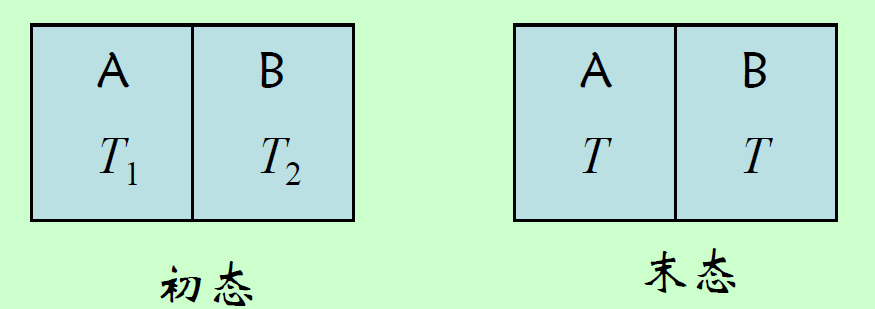
\includegraphics[width=0.55\textwidth]{passing_heat.png}
  \caption{热量传递示意图}
  \label{fig:passing_heat}
\end{figure}

\subsubsection{绝热过程与泊松方程}

对理想气体的准静态绝热过程，由 $\mathrm{d}Q=0$ 得：
\begin{align}
  \mathrm{d}U &= \mathrm{d}A = -p\,\mathrm{d}V = \nu C_{V,m}\,\mathrm{d}T \tag{1}\\
  p\,\mathrm{d}V+V\,\mathrm{d}p &= \nu R\,\mathrm{d}T \tag{2}
\end{align}

消去 $\mathrm{d}T$，并利用 $C_{p,m}=C_{V,m}+R$ 与 $\gamma=\dfrac{C_{p,m}}{C_{V,m}}$（比热容比/绝热指数），得
\[
\frac{\mathrm{d}p}{p}+\gamma\frac{\mathrm{d}V}{V}=0
\]

积分得到\textbf{泊松方程}（绝热过程方程）：
\[
\boxed{pV^{\gamma}=\text{常量}}
\]

由 $pV=\nu RT$ 可得另外两种等价形式：
\[
TV^{\gamma-1}=\text{常量},\qquad \frac{p^{\gamma-1}}{T^{\gamma}}=\text{常量}
\]

\paragraph{绝热过程做功}
\[
W'=-W=\int_{V_1}^{V_2}p\,\mathrm{d}V
=\frac{p_1V_1-p_2V_2}{\gamma-1}
=\frac{\nu R}{\gamma-1}(T_2-T_1)
\]
且满足 $W=C_V(T_2-T_1)$，即\textbf{绝热过程中外界对系统做的功等于系统内能的增量}。

\paragraph{等温线与绝热线斜率比较}
在 $p$-$V$ 图上，等温线 $pV=\text{常量}$ 与绝热线 $pV^{\gamma}=\text{常量}$ 相比，绝热线更陡。

\subsubsection{多方过程}

前面几种准静态过程可统一概括为：
\[
\boxed{pV^{n}=\text{常数}}
\]
其中 $n$ 为\textbf{多方指数}。

\begin{center}
\begin{tabular}{c|c|c}
\hline
过程名称 & 多方指数 $n$ & 过程方程 \\
\hline
等压过程 & $0$ & $p=\text{常量}$ \\
等温过程 & $1$ & $pV=\text{常量}$ \\
绝热过程 & $\gamma$ & $pV^{\gamma}=\text{常量}$ \\
等体过程 & $\infty$ & $V=\text{常量}$ \\
\hline
\end{tabular}
\end{center}

\paragraph{多方过程的主要公式}
\begin{align*}
  TV^{n-1}&=\text{常量},\qquad \frac{p^{n-1}}{T^{n}}=\text{常量}\\[4pt]
  W&=\frac{p_2V_2-p_1V_1}{n-1}=\frac{\nu R}{n-1}(T_2-T_1)\\[4pt]
  \Delta U&=C_V(T_2-T_1)\\[4pt]
  Q&=C_n(T_2-T_1)\\[4pt]
  C_n&=C_V-\frac{\nu R}{n-1}=\frac{n-\gamma}{n-1}C_V
\end{align*}

% [插图：多方过程在 p-V 图上的汇总示意图]
\begin{figure}[htbp]
  \centering
  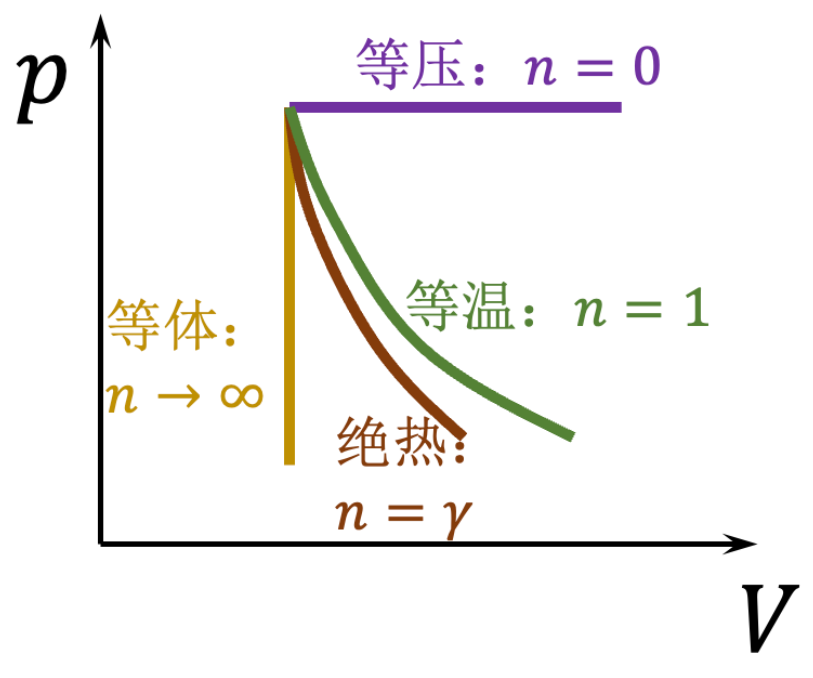
\includegraphics[width=0.7\textwidth]{polytropic_process.png}
  \caption{多方过程在 $p$-$V$ 图上的示意图}
  \label{fig:polytropic_process}
\end{figure}

\subsubsection{大气绝热递减率}

\paragraph{干绝热递减率（DALR）}
将大气视为理想气体，在绝热上升过程中：
\[
\frac{\mathrm{d}T}{\mathrm{d}z}=-\frac{\gamma-1}{\gamma}\frac{Mg}{R}\approx -9.8\ \mathrm{K/km}
\]

温度随高度的分布：
\[
T(z)=T_0\left[1-\left(\frac{Mg}{RT_0}\frac{\gamma-1}{\gamma}\right)z\right]^{\frac{\gamma}{\gamma-1}}
\]
相应的压强公式：
\[
p(z)=p_0\left[1-\left(\frac{Mg}{RT_0}\frac{\gamma-1}{\gamma}\right)z\right]^{\frac{\gamma}{\gamma-1}}
\]
当 $\gamma\to 1$ 时，回到等温大气压强公式 $p=p_0\exp[-mgz/(k_BT)]$。

\paragraph{饱和绝热递减率（SALR）}
考虑含水蒸气的湿空气，上升过程中水蒸气凝结放热。对 $1\ \mathrm{mol}$ 湿空气：
\[
C_p^{\mathrm{mol}}\,\mathrm{d}T=-\Lambda^{\mathrm{mol}}\,\mathrm{d}\nu_w+RT\frac{\mathrm{d}p}{p}
\]
推导得：
\[
\frac{\mathrm{d}T}{\mathrm{d}z}
=-\frac{\gamma-1}{\gamma}\frac{Mg}{R}\left(1+\frac{\Lambda^{\mathrm{mol}}}{C_p^{\mathrm{mol}}T}\frac{\mathrm{d}\nu_w}{\mathrm{d}z}\right)
\]
由于 $\dfrac{\mathrm{d}\nu_w}{\mathrm{d}z}<0$（随高度增加水汽减少），故
\[
\boxed{|\mathrm{SALR}|<|\mathrm{DALR}|}
\]


% ============================================================
\subsection{循环过程与热机}
% ============================================================

\subsubsection{卡诺循环}

由两个\textbf{等温过程}和两个\textbf{绝热过程}组成的理想循环。

\paragraph{正卡诺循环（热机）}
\begin{itemize}[leftmargin=2em]
  \item $A\to B$：等温膨胀，吸热 $Q_1$，对外做功；
  \item $B\to C$：绝热膨胀，对外做功；
  \item $C\to D$：等温压缩，放热 $Q'_2$，对系统做功；
  \item $D\to A$：绝热压缩，对系统做功。
\end{itemize}

吸热量与放热量：
\[
Q_1=\nu RT_1\ln\frac{V_B}{V_A},\qquad 
Q'_2=\nu RT_2\ln\frac{V_C}{V_D}
\]

利用绝热过程 $TV^{\gamma-1}=\text{常量}$ 可得 $V_B/V_A=V_C/V_D$，于是\textbf{卡诺热机效率}：
\[
\boxed{\eta=\frac{W'}{Q_1}=1-\frac{Q'_2}{Q_1}=1-\frac{T_2}{T_1}}
\]
\textbf{结论}：理想气体卡诺热机的效率只取决于高低温热源温度，与工作物质无关。

\paragraph{逆卡诺循环（制冷机）}
制冷系数：
\[
\boxed{\varepsilon=\frac{Q_2}{A}=\frac{Q_2}{Q'_1-Q_2}=\frac{T_2}{T_1-T_2}}
\]

\paragraph{卡诺循环的意义}
实际热机（如空气喷气发动机效率约 $60\%$，蒸汽机约 $40\%$）远低于理想极限。卡诺循环为理想循环，\textbf{指出了提高热机效率的方向}。

% [插图：卡诺循环 p-V 图，标注 $Q_1,Q_2,T_1,T_2$]
\begin{figure}[htbp]
  \centering
  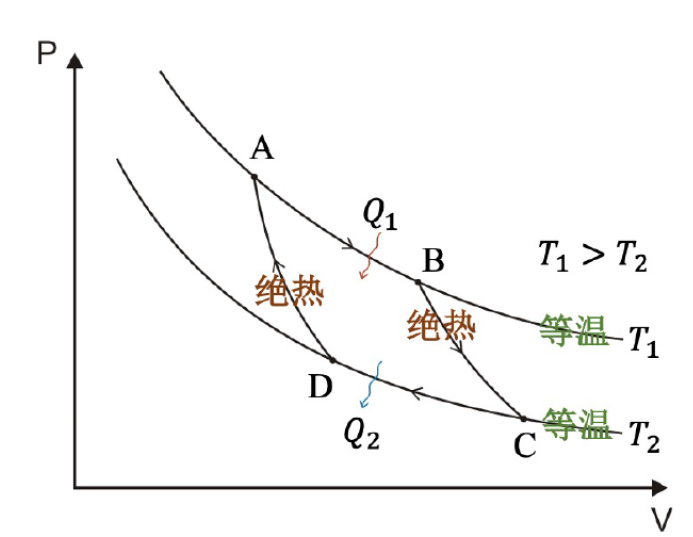
\includegraphics[width=0.45\textwidth]{cardano_cycle.png}
  \caption{卡诺循环 p-V 图}
  \label{fig:cardano_cycle}
\end{figure}

\paragraph{1. 奥托循环（等体加热循环）}
四冲程汽油机的工作循环，由两个等体过程和两个绝热过程构成。
\begin{itemize}[leftmargin=2em]
  \item $1\to 2$：绝热压缩（达到燃点）；
  \item $2\to 3$：等体燃烧吸热；
  \item $3\to 4$：绝热膨胀；
  \item $4\to 1$：等体放热（排气）。
\end{itemize}

吸热与放热：
\[
Q_1=\nu C_{V,m}(T_3-T_2),\qquad Q_2=\nu C_{V,m}(T_4-T_1)
\]

利用绝热关系 $T_2/T_1=T_3/T_4=(V_1/V_2)^{\gamma-1}=r^{\gamma-1}$（$r$ 为绝热压缩比），得\textbf{奥托循环效率}：
\[
\boxed{\eta=1-\frac{T_1}{T_2}=1-\frac{1}{r^{\gamma-1}}}
\]

% [插图：奥托循环 p-V 图，标注四个过程]
\begin{figure}[htbp]
  \centering
  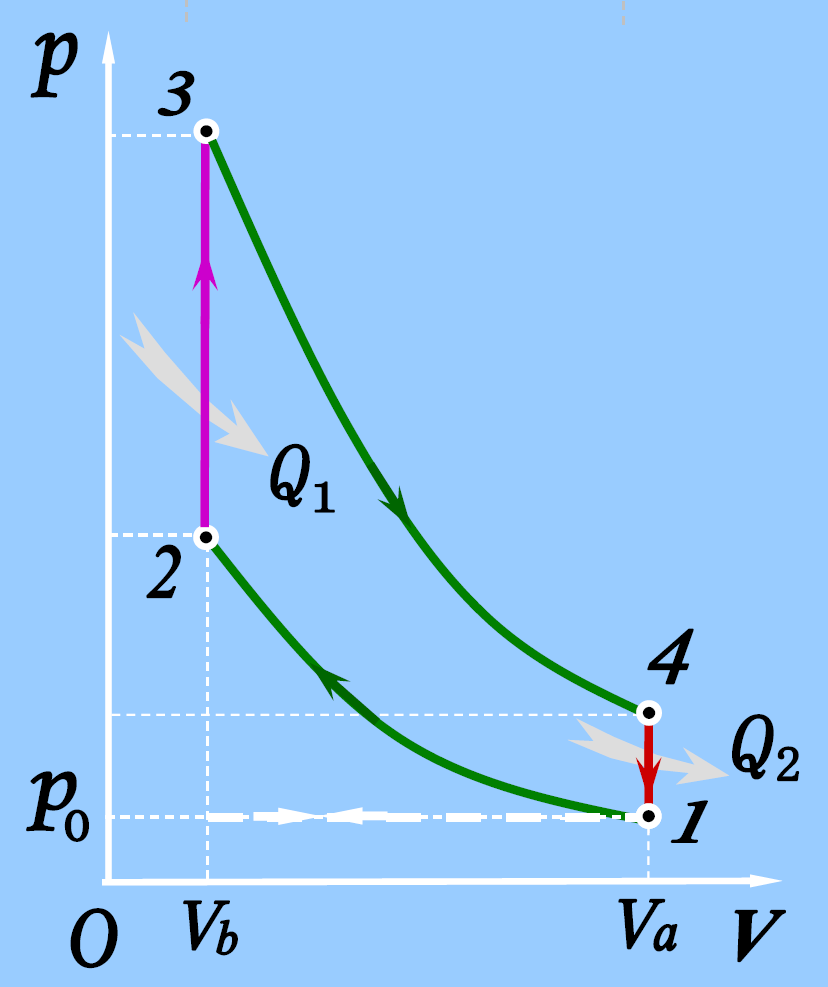
\includegraphics[width=0.45\textwidth]{torque_cycle.png}
  \caption{奥托循环 p-V 图}
  \label{fig:torque_cycle}
\end{figure}

\paragraph{2. 狄塞尔循环（等压加热循环）}
四冲程柴油机的工作循环，由一个等压、一个等体和两个绝热过程构成。
\begin{itemize}[leftmargin=2em]
  \item $1\to 2$：空气绝热压缩；
  \item $2\to 3$：等压燃烧吸热；
  \item $3\to 4$：绝热膨胀；
  \item $4\to 1$：等体放热（排气）。
\end{itemize}

定义：
\begin{itemize}[leftmargin=2em]
  \item 绝热压缩比：$r=\dfrac{V_1}{V_2}$
  \item 定压膨胀比：$\rho=\dfrac{V_3}{V_2}$
  \item 绝热膨胀比：$\delta=\dfrac{V_1}{V_3}=\dfrac{r}{\rho}$
\end{itemize}

\textbf{狄塞尔循环效率}：
\[
\boxed{\eta=1-\frac{1}{r^{\gamma-1}}\frac{\rho^{\gamma}-1}{\gamma(\rho-1)}}
\]
\textbf{结论}：绝热压缩比 $r$ 越大，效率越高。

% [插图：狄塞尔循环 p-V 图]
\begin{figure}[htbp]
  \centering
  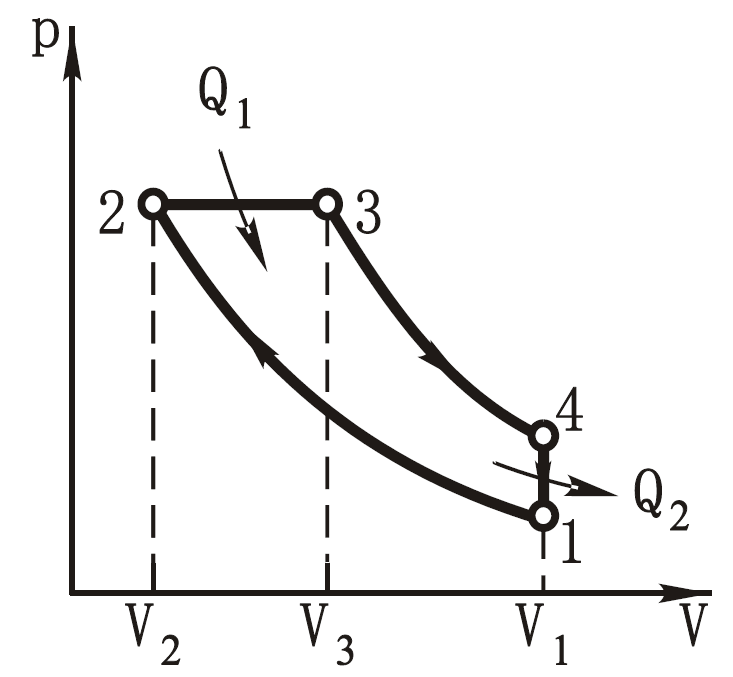
\includegraphics[width=0.45\textwidth]{diesel_cycle.png}
  \caption{狄塞尔循环 p-V 图}
  \label{fig:diesel_cycle}
\end{figure}


\subsubsection{逆向斯特林循环（制冷循环）}

由两个等体和两个等温过程构成的循环。
\begin{itemize}[leftmargin=2em]
  \item $1\to 2$：等温压缩放热；
  \item $2\to 3$：等体吸热；
  \item $3\to 4$：等温膨胀吸热；
  \item $4\to 1$：等体放热。
\end{itemize}

在两个等体过程中与外界交换的热量代数和为零。吸热与放热：
\[
Q_2=\nu RT_2\ln\frac{V_1}{V_2},\qquad Q_1=\nu RT_1\ln\frac{V_1}{V_2}
\]

由热力学第一定律，外界做功 $A=Q_1-Q_2=\nu R(T_1-T_2)\ln\dfrac{V_1}{V_2}$。

\textbf{制冷系数}：
\[
\boxed{\varepsilon=\frac{Q_2}{A}=\frac{T_2}{T_1-T_2}}
\]
\textbf{结论}：逆向斯特林循环的制冷系数与逆向卡诺循环一致。回热式制冷机具有较高的制冷效率。

% [插图：逆向斯特林循环 p-V 图]
\begin{figure}[htbp]
  \centering
  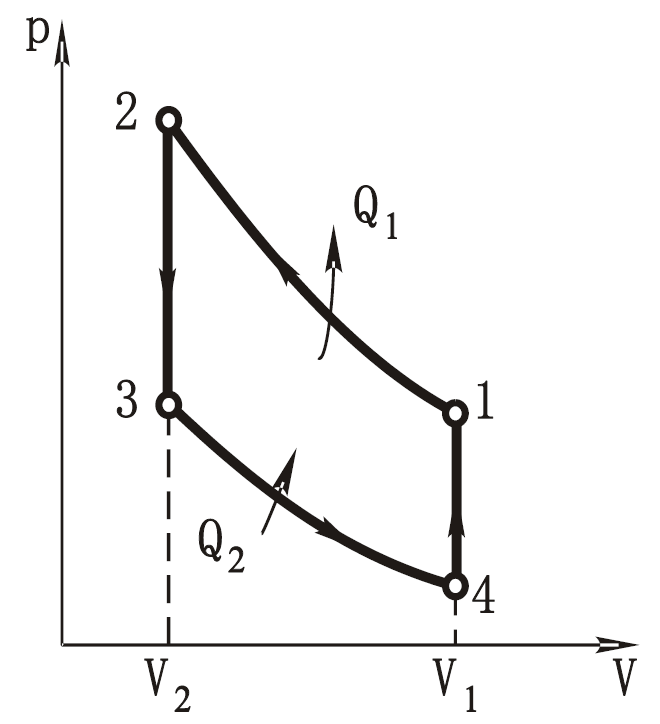
\includegraphics[width=0.45\textwidth]{reverse_sterling_cycle.png}
  \caption{逆向斯特林循环 p-V 图}
  \label{fig:reverse_sterling_cycle}
\end{figure}


% ============================================================
\subsection{习题解答}
% ============================================================

\subsubsection{题 4.1}

\textbf{题目}：试在 $p$-$V$ 图上画出以下理想气体系统完成的准静态过程：
(1) $p=kV$；(2) $p=kT$；(3) $V=kT$，其中 $k$ 为满足各自要求的常量。并计算当系统体积由 $V_1$ 变至 $V_2$ 时，上述三过程中系统对外界所作的功。

\begin{thoughts}
  直接做图像计算即可。
\end{thoughts}

\textbf{解答}：

(1) \textbf{作图}
\begin{itemize}[leftmargin=2em]
  \item 过程 (1)：$p=kV$，在 $p$-$V$ 图上为过原点的直线（题 4.1 解答图 (a)）。
  \item 过程 (2)：$p=kT$，由 $pV=\nu RT$ 得 $V=\dfrac{\nu R}{k}=\text{常量}$，为等体过程（题 4.1 解答图 (b)）。
  \item 过程 (3)：$V=kT$，由 $pV=\nu RT$ 得 $p=\dfrac{\nu R}{k}=\text{常量}$，为等压过程（题 4.1 解答图 (c)）。
\end{itemize}

% [插图：题 4.1 解答图 (a)(b)(c)，分别标注三条曲线]
\begin{figure}[htbp]
  \centering
  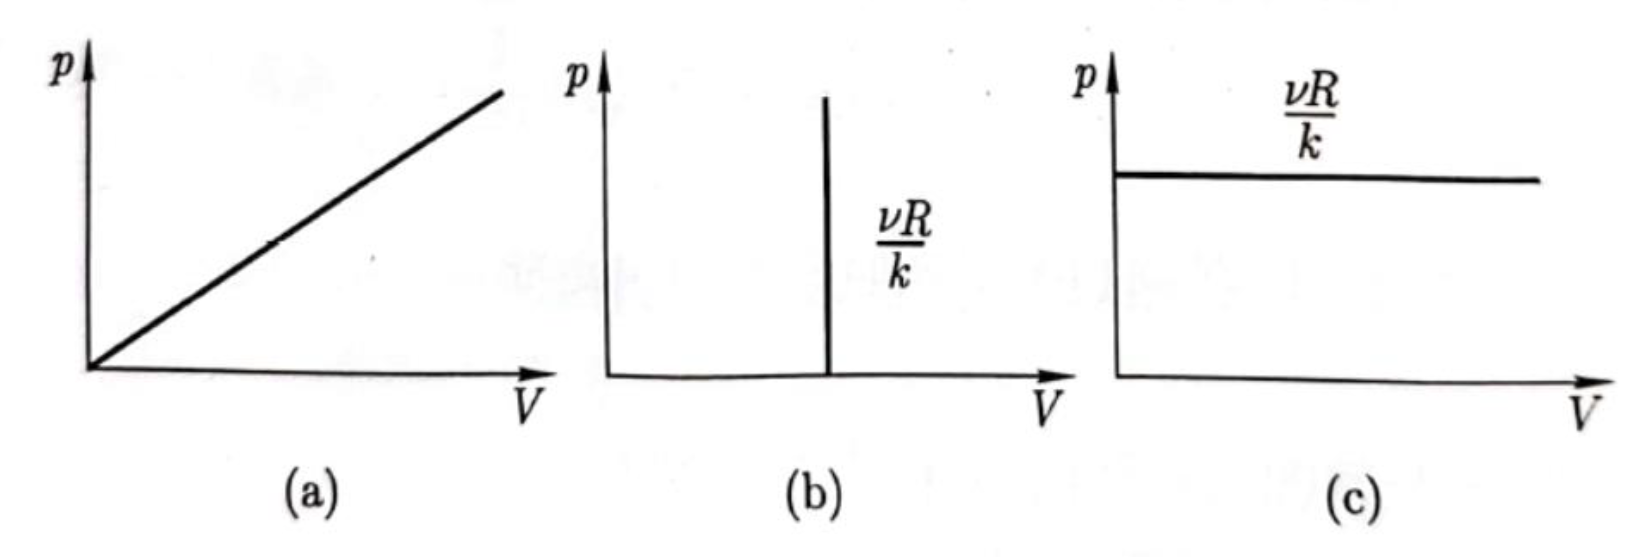
\includegraphics[width=0.6\textwidth]{4_1.png}
  \caption{题 4.1 解答图 (a)(b)(c)，分别标注三条曲线}
  \label{fig:4_1}
\end{figure}


(2) \textbf{计算系统对外界所做的功}
\begin{align*}
  \text{过程 (1)}:\quad W'&=\int_{V_1}^{V_2}p\,\mathrm{d}V=\int_{V_1}^{V_2}kV\,\mathrm{d}V
  =\frac{1}{2}k\bigl(V_2^2-V_1^2\bigr)\\[4pt]
  \text{过程 (2)}:\quad W'&=\int p\,\mathrm{d}V=0\qquad(\because \mathrm{d}V=0)\\[4pt]
  \text{过程 (3)}:\quad W'&=\int_{V_1}^{V_2}p\,\mathrm{d}V
  =\frac{\nu R}{k}\bigl(V_2-V_1\bigr)
\end{align*}

\textbf{结果}：三过程做功分别为
\[
\boxed{\frac{1}{2}k\bigl(V_2^2-V_1^2\bigr),\quad 0,\quad \frac{\nu R}{k}\bigl(V_2-V_1\bigr)}
\]

\subsubsection{题 4.3}

\textbf{题目}：一气体系统的定压摩尔热容量随温度改变的规律为 $C_p=a+bT-cT^2$，其中 $a,b,c$ 是常量。当 $n\ \mathrm{mol}$ 气体经一个等压过程使温度从 $T_1$ 变到 $T_2$ 时，气体从外界吸收的热量为多少？

\begin{thoughts}
  利用$\triangle Q = \triangle U = C_P \triangle T$，注意是等压摩尔热容，所以需要乘物质的量
\end{thoughts}

\textbf{解答}：
\[
Q=\int_{T_1}^{T_2}C_p\,n\,\mathrm{d}T
=n\int_{T_1}^{T_2}\bigl(a+bT-cT^2\bigr)\,\mathrm{d}T
\]

积分得：
\[
\boxed{Q=n\left[a(T_2-T_1)+\frac{b}{2}\bigl(T_2^2-T_1^2\bigr)-\frac{c}{3}\bigl(T_2^3-T_1^3\bigr)\right]}
\]

\subsubsection{题 4.7}

\textbf{题目}：$1.0\ \mathrm{g}$ 氮气原来的温度和压强分别为 $423\ \mathrm{K}$ 和 $5.066\times 10^5\ \mathrm{Pa}$，经准静态绝热膨胀后，体积变为原来的两倍。试确定在这一过程中气体对外界所作的功。

\begin{thoughts}
  利用公式$$W=\frac{P_2V_2-P_1V_1}{\gamma-1}=\frac{\nu R}{\gamma-1} (T_2-T_1)$$，得到以下重要结果
\end{thoughts}

\textbf{解答}：将氮气视为理想气体，由绝热方程 $pV^{\gamma}=p_1V_1^{\gamma}$ 得
\[
p=\frac{p_1V_1^{\gamma}}{V^{\gamma}}
\]

过程中对外做功：
\[
W'=\int_{V_1}^{V_2}p\,\mathrm{d}V
=\frac{p_1V_1^{\gamma}}{1-\gamma}\bigl(V_2^{1-\gamma}-V_1^{1-\gamma}\bigr)
=\frac{1}{1-\gamma}\bigl(p_2V_2-p_1V_1\bigr)
=\frac{\nu R}{\gamma-1}\bigl(T_1-T_2\bigr)
\]

由 $T_1V_1^{\gamma-1}=T_2V_2^{\gamma-1}$ 及 $V_2=2V_1$，$\gamma=\dfrac{7}{5}$（双原子分子），代入数据 $T_1=423\ \mathrm{K}$，$M=1\ \mathrm{g}$，$R=8.31\ \mathrm{J/(mol\cdot K)}$：
\[
W'=\frac{(1\times 10^{-3})\times 8.31\times 423}{\dfrac{7}{5}-1}
\left[1-\left(\frac{1}{2}\right)^{\frac{7}{5}-1}\right]
\]

\[
\boxed{W'\approx 76\ \mathrm{J}}
\]

\subsubsection{题 4.9}

\textbf{题目}：在原子弹爆炸后 $0.1\ \mathrm{s}$ 所出现的“火球”是半径约 $15\ \mathrm{m}$、温度为 $3000\ \mathrm{K}$ 的气体球，试确定温度变为 $300\ \mathrm{K}$ 时，“火球”的半径大约为多大？

\begin{thoughts}
  绝热过程$$PV^\gamma = \text{Const} \Rightarrow TV^{\gamma-1} = \text{Const}$$
\end{thoughts}

\textbf{解答}：将“火球”膨胀视为绝热过程，满足
\[
TV^{\gamma-1}=T_1V_1^{\gamma-1}
\]

因 $V=\dfrac{4}{3}\pi R^3$，故
\[
T_1R_1^{3(\gamma-1)}=T_2R_2^{3(\gamma-1)}
\quad\Longrightarrow\quad
R_2=\left(\frac{T_1}{T_2}\right)^{\frac{1}{3(\gamma-1)}}R_1
\]

取空气（双原子分子）$\gamma=\dfrac{7}{5}$，$T_1=3000\ \mathrm{K}$，$T_2=300\ \mathrm{K}$，$R_1=15\ \mathrm{m}$：
\[
R_2=\left(\frac{3000}{300}\right)^{\frac{1}{3\times 0.4}}\times 15
=10^{\frac{5}{6}}\times 15\approx 69.5\ \mathrm{m}
\]

% [注：原题图片中后续还有关于非相对论模型与内能的讨论，此处保留核心公式]

\subsubsection{题 4.12}

\textbf{题目}：两端开口的 U 形管中注入水银，全长 $h$。
(1) 将一边压下后使水银振荡，证明不计摩擦时周期 $\tau_1=2\pi\sqrt{\dfrac{h}{2g}}$。
(2) 左侧封闭气柱高 $l$，作准静态绝热振荡，气压计水银柱高 $h_0$，证明周期变为
$\tau_2=2\pi\sqrt{\dfrac{h}{2g+\gamma h_0g/l}}$。

\begin{thoughts}
  对上升部分柱体受力分析，列微分方程，利用关系$$\omega^2x + a=0$$
\end{thoughts}

\textbf{证明}：

(1) 设水银密度 $\rho$，截面积 $S$。偏离平衡位置高度 $x$ 时，回复力
\[
F=(\rho\cdot 2x\cdot S)g
\]
水银质量 $m=\rho hS$，由 $F=m\ddot{x}$ 得
\[
\ddot{x}=\frac{2g}{h}x
\]
与简谐振动 $\ddot{x}=\omega^2x$ 比较，$\omega=\sqrt{2g/h}$，故
\[
\boxed{\tau_1=2\pi\sqrt{\frac{h}{2g}}}
\]

(2) 左侧封闭，偏离 $x$ 时左侧压强 $p$，大气压 $p_0=\rho gh_0$，回复力
\[
F=(p_0+\rho g\cdot 2x-p)S=\rho hS\ddot{x}
\]
封闭气体经历绝热过程：$p(l+x)^{\gamma}=p_0l^{\gamma}$，故
\[
p\approx p_0\left(1-\gamma\frac{x}{l}\right)
\]
代入得
\[
\ddot{x}=\frac{2g+\gamma\dfrac{h_0}{l}g}{h}x
\]
于是
\[
\boxed{\tau_2=2\pi\sqrt{\frac{h}{2g+\gamma h_0g/l}}}
\]

% [插图：U 形管水银柱振荡示意图]
\begin{figure}[htbp]
  \centering
  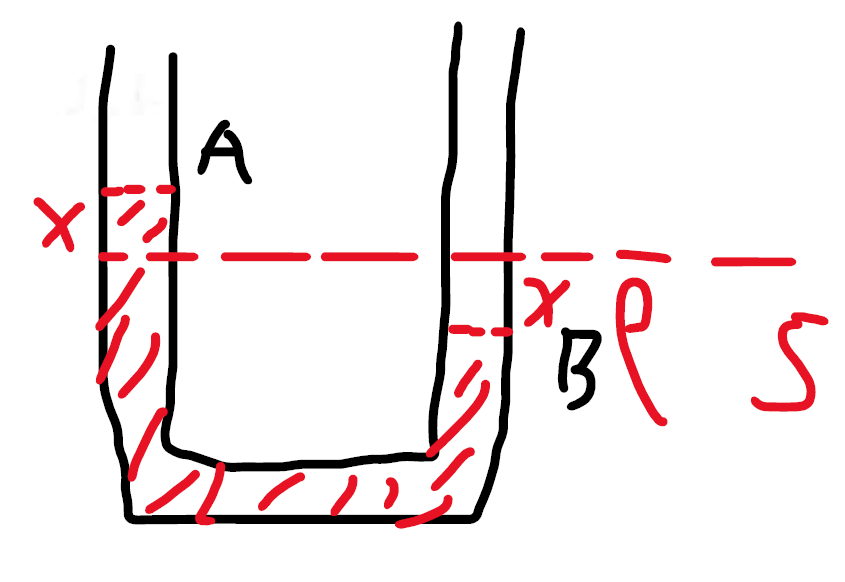
\includegraphics[width=0.4\textwidth]{4_12.png}
  \caption{题 4.12 U 形管水银柱振荡示意图}
  \label{fig:4_12}
\end{figure}

\subsubsection{题 4.16（大气与云层问题）}

\textbf{题目}：如图所示，在一山峰的两侧建有气象观测站 $M_1,M_4$，山顶建有观测站 $M_3$，一侧山坡上建有观测站 $M_2$。通常，潮湿空气可以沿着山坡持续上升并流到另一侧。某日，观测站 $M_1$ 测得其附近的大气压强为 $p_1=100\ \mathrm{kPa}$、气温为 $t_1=20^{\circ}\mathrm{C}$，$M_4$ 测得大气压强也为 $100\ \mathrm{kPa}$，$M_3$ 测得的大气压强为 $p_3=70\ \mathrm{kPa}$，$M_2$ 测得大气压强为 $p_2=84.5\ \mathrm{kPa}$，并发现在其所处高度开始有云形成。潮湿空气继续上升，经约 $25\ \mathrm{min}$ 后到达山顶，并且在这段过程中其中的水蒸气凝结成雨而落下。记每平方米面积上空的潮湿空气的质量为 $2000\ \mathrm{kg}$，每 $\mathrm{kg}$ 潮湿空气可凝结出 $2.45\ \mathrm{g}$ 雨水，水的汽化热为 $2.5\times 10^{3}\ \mathrm{kJ/kg}$（即 $2.5\times 10^{6}\ \mathrm{J/kg}$），并且空气可以近似为理想气体。

\begin{enumerate}
    \item[(1)] 假设空气密度随高度增加而线性减小，试确定云底距离地面的高度。
    \item[(2)] 试确定云底处的气温。
    \item[(3)] 试确定山顶的观测站 $M_3$ 测得的气温。
    \item[(4)] 假设在观测站 $M_2$ 与 $M_3$ 之间的降雨均匀，并记每小时内每平方米面积内降落 $1\ \mathrm{kg}$ 雨水为 $1\ \mathrm{mm}$ 的降雨量，试确定这两个观测站之间的降雨量。
    \item[(5)] 在 $M_4$ 处进行观测，测得的气温很可能为多少 $^{\circ}\mathrm{C}$？与 $M_1$ 处的相比，这里的空气有何特点？
\end{enumerate}

\begin{thoughts}
  由等温模型分析知道$\delta P$和$\delta z$的关系，而$PV^{\gamma - 1} = Const$，这导致了$\frac{dT}{dz}$的等式\\
  对温度变化的贡献除了高度上升还有水蒸气液化放热。考虑单位质量内有$m_\omega$水蒸气液化，则由能量守恒可知液化后温度变化值，综合可得结果\\
  降水量用总降水平均时间和面积即可
\end{thoughts}

\textbf{解答}：

(1) \textbf{云底距地面的高度}

因为高度为 $z$ 处的大气处于力学平衡时，压强变化量 $\mathrm{d}p$ 与高度改变量 $\mathrm{d}z$ 间的关系为
\[
\frac{\mathrm{d}p}{\mathrm{d}z}=-\rho g .
\]
依题意，记空气密度随高度增加而线性减小的函数关系为
\[
\rho=\rho_0(1-\chi z),
\]
其中 $\rho_0$ 为水平地面（即高度为 $0$ 的观测站 $M_1$ 处）上的空气密度，$\chi$ 为空气的密度递减率。代入静力学平衡方程得
\[
\mathrm{d}p=-\rho_0(1-\chi z)g\,\mathrm{d}z.
\]

另一方面，因为大气密度可以由大气的组分粒子的质量 $m$ 和其数密度表示为 $\rho=nm$，则由上式可得大气的分子数密度随高度变化的行为为 $n=n_0(1-\chi z)$，于是有
\[
\chi z=\frac{n_0-n_z}{n_0}.
\]
将上式代入积分式则得
\[
p_z-p_0=-\rho_0 g\!\left(z-\frac{n_0-n_z}{2n_0}z\right).
\]
由之可得
\[
z=\frac{p_0-p_z}{\rho_0 g}\cdot\frac{2n_0}{n_0+n_z}.
\]

由理想气体状态方程 $p=nk_{\mathrm{B}}T$ 知，观测站 $M_1$ 处（$z=0$，$p_0=p_1$）的空气分子数密度为
\[
n_0=n_1=\frac{p_1}{k_{\mathrm{B}}T_1},
\]
观测站 $M_2$ 处（$p_z=p_2$）的空气分子数密度为
\[
n_z=n_2=\frac{p_2}{k_{\mathrm{B}}T_2}.
\]
将 $n_1$ 和 $n_2$ 的表达式代入上式，并利用 $\rho_0=p_1\mu/(RT_1)$（$\mu$ 为空气摩尔质量），整理得
\[
z=\frac{R(p_1-p_2)}{\mu g}\cdot\frac{2T_1T_2}{p_1T_2+p_2T_1}.
\]
式中 $R=8.31\ \mathrm{J/(mol\cdot K)}$ 为普适气体常量，$\mu=29\times 10^{-3}\ \mathrm{kg/mol}$，$g=9.8\ \mathrm{m/s^2}$，而 $T_2$ 为云底处的气温（见第 (2) 问，$T_2=279.38\ \mathrm{K}$）。

将各数据代入：
\[
z_{M_2}=\frac{8.31\times(100-84.5)\times 10^3}{(29\times 10^{-3})\times 9.8}
\times\frac{2\times 293.15\times 279.38}{(100\times 10^3)\times 279.38+(84.5\times 10^3)\times 293.15}
\approx 1.408\times 10^{3}\ \mathrm{m}.
\]
即
\[
\boxed{z_{M_2}\approx 1.41\times 10^{3}\ \mathrm{m}\;(1408\ \mathrm{m})}.
\]

(2) \textbf{云底处的气温}

记观测站 $M_1$ 测得的大气压强为 $p_1$、温度为 $T_1$，$M_2$ 测得的大气压强为 $p_2$、温度为 $T_2$。依题意，$T_2$ 即为待求的云层底处的气温。

由于通常的大气中的过程都来不及与外界交换热量，因此可以认为是\textbf{绝热过程}。将大气近似为理想气体，由绝热过程方程 $pV^{\gamma}=\text{常量}$（其中 $\gamma$ 为气体的绝热指数）和理想气体状态方程 $pV=\nu RT$，消去 $V$ 可得
\[
\frac{T^{\gamma}}{p^{\gamma-1}}=\text{常量}.
\]
于是
\[
\frac{T_1^{\gamma}}{p_1^{\gamma-1}}=\frac{T_2^{\gamma}}{p_2^{\gamma-1}},
\qquad\Longrightarrow\qquad
T_2=\left(\frac{p_2}{p_1}\right)^{\frac{\gamma-1}{\gamma}}T_1.
\]

因为空气的主要成分为氮气和氧气，即空气分子可以近似为双原子分子，于是由绝热指数的定义知
\[
\gamma=\frac{C_{p,\mathrm{m}}}{C_{V,\mathrm{m}}}=\frac{\frac{7}{2}R}{\frac{5}{2}R}=\frac{7}{5}=1.4.
\]

将 $\gamma=1.4$，$T_1=273.15+20=293.15\ \mathrm{K}$，$p_1=100\ \mathrm{kPa}$，$p_2=84.5\ \mathrm{kPa}$ 代入得
\[
T_2=\left(\frac{84.5\times 10^3}{100\times 10^3}\right)^{\frac{1.4-1}{1.4}}\times 293.15
=279.38\ \mathrm{K}=6.23^{\circ}\mathrm{C}.
\]
故云层底处的气温为
\[
\boxed{T_2\approx 279.4\ \mathrm{K}\;(6.23^{\circ}\mathrm{C})}.
\]

(3) \textbf{山顶观测站 $M_3$ 测得的气温}

依题意，观测站 $M_2$ 与 $M_3$ 之间的大气可以近似为包含饱和水蒸气的大气，并且饱和水蒸气凝结成水而形成降雨。由于潮湿大气凝结成水时放出热量，因此观测站 $M_3$ 附近干燥大气的温度可以认为由两方面因素决定：

\begin{itemize}
    \item 一方面是随着高度逐渐增加、压强逐渐减小而引起的\textbf{绝热降温过程}，记仅由该因素使 $M_3$ 附近大气达到的温度为 $T_3^{\mathrm{S}}$；
    \item 另一方面是观测站 $M_2$ 附近的干燥大气吸收水蒸气凝结成水时放出的热量而发生的\textbf{等压升温过程}，记该因素使 $M_3$ 附近大气的温度改变为 $T_3^{\mathrm{IB}}$。
\end{itemize}

\textbf{绝热降温所致温度 $T_3^{\mathrm{S}}$}

按照与第 (2) 问相同的方法，有
\[
T_3^{\mathrm{S}}=\left(\frac{p_3}{p_1}\right)^{\frac{\gamma-1}{\gamma}}T_1
=\left(\frac{70\times 10^3}{100\times 10^3}\right)^{\frac{0.4}{1.4}}\times 293.15
=264.75\ \mathrm{K}.
\]

\textbf{凝结放热所致升温 $T_3^{\mathrm{IB}}$}

对于后一种因素引起的温度改变，依题意考虑单位质量包含饱和水蒸气的大气，记由之凝结出的水的质量为 $m_w=2.45\times 10^{-3}\ \mathrm{kg}$，则其中干燥大气的质量为 $1-m_w$。记水蒸气的凝结热（水的汽化热）为 $l_{\mathrm{v}}=2.5\times 10^{6}\ \mathrm{J/kg}$，干燥大气的定压比热容为 $c_p$，则由\textbf{能量守恒定律}得
\[
l_{\mathrm{v}}\,m_w=(1-m_w)\,c_p\,T_3^{\mathrm{IB}}.
\]

因为 $c_p=\dfrac{C_{p,\mathrm{m}}}{\mu}=\dfrac{\frac{7}{2}R}{\mu}=\dfrac{7R}{2\mu}$，于是
\[
T_3^{\mathrm{IB}}=\frac{l_{\mathrm{v}}\,m_w}{(1-m_w)\,c_p}
=\frac{2\mu\,l_{\mathrm{v}}\,m_w}{(1-m_w)\cdot 7R}.
\]

将已知数据代入上式：
\[
T_3^{\mathrm{IB}}=\frac{2\times(29\times 10^{-3})\times(2.5\times 10^{6})\times(2.45\times 10^{-3})}
{\bigl[1-(2.45\times 10^{-3})\bigr]\times 7\times 8.31}
\approx 6.12\ \mathrm{K}.
\]

\textbf{山顶总温度}

\[
T_3=T_3^{\mathrm{S}}+T_3^{\mathrm{IB}}=264.75+6.12=270.87\ \mathrm{K},
\]
即
\[
\boxed{T_3\approx 270.9\ \mathrm{K}\;(-2.28^{\circ}\mathrm{C})}.
\]

(4) \textbf{两观测站 $M_2$ 与 $M_3$ 之间的降雨量}

依题意，记单位面积上空的潮湿空气的质量为 $M_{\mathrm{S}}=2000\ \mathrm{kg/m^2}$，则由之可凝结出的水的质量为 $M_{\mathrm{S}}\,m_w$。因为在题设时间 $t=25\ \mathrm{min}=\dfrac{25}{60}\ \mathrm{h}$ 内降雨均匀，则单位时间在单位面积上凝结的雨水的质量为
\[
M=\frac{M_{\mathrm{S}}\,m_w}{t}.
\]

将已知数据代入上式，得
\[
M=\frac{2000\times(2.45\times 10^{-3})}{\frac{25}{60}}
\approx 11.70\ \mathrm{kg/(m^2\cdot h)}.
\]

按题中“每小时内每平方米面积内降落 $1\ \mathrm{kg}$ 雨水为 $1\ \mathrm{mm}$ 的降雨量”的定义，该平均降雨强度对应的等效降雨量为
\[
\boxed{11.76\ \mathrm{mm}}.
\]
（注：若指该时段内的总降水深度，则 $M_{\mathrm{S}}\,m_w=4.9\ \mathrm{kg/m^2}$，对应总降雨深度约 $4.9\ \mathrm{mm}$。）

(5) \textbf{$M_4$ 处的气温及空气特点}

依题意，观测站 $M_3$ 与 $M_4$ 之间的大气中的过程为\textbf{绝热过程}（空气从山顶流向另一侧山脚，来不及与外界交换热量），于是有
\[
T_4=\left(\frac{p_4}{p_3}\right)^{\frac{\gamma-1}{\gamma}}T_3
=\left(\frac{100\times 10^3}{70\times 10^3}\right)^{\frac{0.4}{1.4}}\times 270.87
\approx 299.93\ \mathrm{K}=26.78^{\circ}\mathrm{C}.
\]

所以，在 $M_4$ 处进行观测，测得的气温很可能为
\[
\boxed{26.78^{\circ}\mathrm{C}}.
\]

与 $M_1$ 处相比，这里的空气\textbf{温度较高}（$26.78^{\circ}\mathrm{C}>20^{\circ}\mathrm{C}$），\textbf{湿度较小}，因为大气中的水蒸气在翻越山顶的过程中已经凝结成水析出。这正是典型的\textbf{焚风（Föhn）效应}。

% [插图：题 4.16 山峰与云层示意图]
\begin{figure}[htbp]
  \centering
  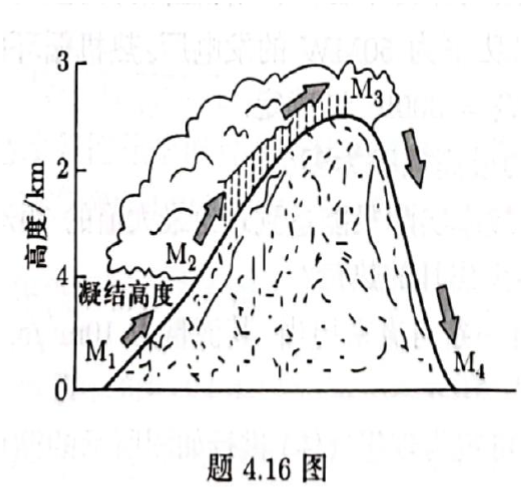
\includegraphics[width=0.4\textwidth]{4_16.png}
  \caption{题 4.16 山峰与云层示意图}
  \label{fig:4_16}
\end{figure}

\subsubsection{题 4.18（理想气体多方过程）}

\textbf{题目}：一定量氧气，初始状态为 $p_1=1.0\ \mathrm{atm}=1\times 10^5\ \mathrm{Pa}$，$V_1=2.3\ \mathrm{L}=2.3\times 10^{-3}\ \mathrm{m^3}$，$t_1=26^{\circ}\mathrm{C}$；经一多方过程达到 $p_2=0.50\ \mathrm{atm}=5\times 10^4\ \mathrm{Pa}$，$V_2=4.1\ \mathrm{L}=4.1\times 10^{-3}\ \mathrm{m^3}$。试确定：
\begin{enumerate}
    \item[(1)] 多方指数 $n$；
    \item[(2)] 内能的变化量 $\Delta U$；
    \item[(3)] 对外界做的功 $W'$；
    \item[(4)] 吸收的热量 $Q$。
\end{enumerate}

\begin{thoughts}
  多方过程系数用$PV^n=\text{Const}$确定，内能变化量$U=C_V(T_2-T_1)$，对外界做的功$W'=\frac{\nu R}{n-1}(T_2-T_1)$，吸收热量$Q=C_n(T_2-T_1)=\frac{n-\gamma}{n-1}C_V$，其中$\gamma = 1 + \frac{R}{C_V}$
\end{thoughts}

\textbf{解答}：

\textbf{(1) 多方指数 $n$}

将这些氧气近似为理想气体，由理想气体多方过程的过程方程
\[
pV^{n}=\text{常量},
\]
得 $p_1V_1^{n}=p_2V_2^{n}$，于是有
\[
\left(\frac{V_1}{V_2}\right)^{n}=\frac{p_2}{p_1}.
\]
对上式两边取对数，得
\[
n\ln\frac{V_1}{V_2}=\ln\frac{p_2}{p_1},
\qquad\Longrightarrow\qquad
n=\frac{\ln(p_2/p_1)}{\ln(V_1/V_2)}.
\]
将已知数据 $p_1=1\times 10^5\ \mathrm{Pa}$，$V_1=2.3\times 10^{-3}\ \mathrm{m^3}$，$p_2=5\times 10^4\ \mathrm{Pa}$，$V_2=4.1\times 10^{-3}\ \mathrm{m^3}$ 代入，得
\[
n=\frac{\ln(5\times 10^4/1\times 10^5)}{\ln(2.3/4.1)}
=\frac{\ln 0.5}{\ln 0.561}
=\frac{\ln 2}{\ln(4.1/2.3)}
\approx 1.2.
\]
故
\[
\boxed{n=1.2}.
\]

\textbf{(2) 内能的变化量 $\Delta U$}

由理想气体状态方程 $pV=\nu RT$，得到状态 1、2 间的状态参量关系
\[
\frac{p_1V_1}{T_1}=\frac{p_2V_2}{T_2},
\qquad\Longrightarrow\qquad
T_2=\frac{p_2V_2}{p_1V_1}\,T_1.
\]
该过程中系统内能的变化量为
\[
\Delta U=\nu C_{V,\mathrm{m}}(T_2-T_1)
=\nu C_{V,\mathrm{m}}T_1\left(\frac{p_2V_2}{p_1V_1}-1\right)
=\frac{C_{V,\mathrm{m}}}{R}\,(p_2V_2-p_1V_1).
\]
因为氧气为双原子气体分子，在题设常温下 $C_{V,\mathrm{m}}=\dfrac{5}{2}R$，于是
\[
\Delta U=\frac{5}{2}(p_2V_2-p_1V_1).
\tag{1}
\]
又由 $pV=\nu RT$ 知 $\nu RT_1=p_1V_1$，将数据代入式 (1)：
\[
\Delta U=\frac{5}{2}\left(5\times 10^4\times 4.1\times 10^{-3}
-1\times 10^5\times 2.3\times 10^{-3}\right)
=\frac{5}{2}(205-230)
=-62.5\ \mathrm{J}.
\]
故
\[
\boxed{\Delta U=-62.5\ \mathrm{J}}.
\]

\textbf{(3) 对外界做的功 $W'$}

由多方过程方程 $pV^{n}=\text{常量}$，可得
\[
p=\frac{p_1V_1^{n}}{V^{n}}.
\]
该过程中氧气对外界所做的功为
\begin{align*}
W'&=\int_{V_1}^{V_2}p\,\mathrm{d}V
=\int_{V_1}^{V_2}p_1V_1^{n}\frac{\mathrm{d}V}{V^{n}}
=p_1V_1^{n}\frac{1}{1-n}\left(V_2^{1-n}-V_1^{1-n}\right) \\[4pt]
&=\frac{1}{1-n}\left(p_2V_2-p_1V_1\right)
=\frac{1}{n-1}\left(p_1V_1-p_2V_2\right).
\tag{2}
\end{align*}
将已知数据及 $n=1.2$ 代入式 (2)：
\[
W'=\frac{1}{1.2-1}\left(1\times 10^5\times 2.3\times 10^{-3}
-5\times 10^4\times 4.1\times 10^{-3}\right)
=\frac{1}{0.2}(230-205)
=125\ \mathrm{J}.
\]
故
\[
\boxed{W'=125\ \mathrm{J}}.
\]

\textbf{(4) 吸收的热量 $Q$}

因为氧气的定体摩尔热容为 $C_{V,\mathrm{m}}=\dfrac{5}{2}R$，定压摩尔热容为 $C_{p,\mathrm{m}}=\dfrac{7}{2}R$，则其绝热指数为
\[
\gamma=\frac{C_{p,\mathrm{m}}}{C_{V,\mathrm{m}}}=\frac{7}{5}=1.4.
\]
由多方过程热容公式
\[
C_{n}=\frac{n-\gamma}{n-1}\,C_{V},
\]
得到该多方过程中的热容为
\[
C_{n}=\frac{1.2-\dfrac{7}{5}}{1.2-1}\cdot\nu\frac{5}{2}R
=\frac{1.2-1.4}{0.2}\cdot\frac{5}{2}\nu R
=-\frac{5}{2}\nu R.
\]
那么，该过程吸收的热量为
\begin{align*}
Q&=C_{n}(T_2-T_1)
=-\frac{5}{2}\nu R(T_2-T_1)
=-\frac{5}{2}(p_2V_2-p_1V_1) \\[4pt]
&=-\frac{5}{2}\left(5\times 10^4\times 4.1\times 10^{-3}
-1\times 10^5\times 2.3\times 10^{-3}\right) \\[4pt]
&=62.5\ \mathrm{J}.
\end{align*}
（亦可由热力学第一定律 $Q=\Delta U+W'=-62.5+125=62.5\ \mathrm{J}$ 直接得到。）

故
\[
\boxed{Q=62.5\ \mathrm{J}}.
\]

% [注：数值以教材原始数据为准，此处保留题图所示结果]

\subsubsection{题 4.19（变热容过程）}

\textbf{题目}：证明若理想气体按 $V=a_0/\sqrt{p}$ 的规律膨胀，其中 $a_0$ 为常量，则气体在该过程中的热容 $C$ 可以表示为
\[
C=C_V-\frac{a_0^2}{TV}.
\]
并说明气体的温度随膨胀而变化的行为。

\begin{thoughts}
  本题中气体膨胀为$n=2$的多方过程，$C_n$由上题关系式求解，温度与体积的关系可由压强与体积的关系导出
\end{thoughts}

\textbf{证明}：

由热力学第一定律 $\mathrm{d}U=\mathrm{d}Q+\mathrm{d}W$（其中 $\mathrm{d}W=-p\,\mathrm{d}V$ 为外界对系统做的功），可得
\[
\mathrm{d}Q=\mathrm{d}U+p\,\mathrm{d}V.
\]
对理想气体，$\mathrm{d}U=C_V\,\mathrm{d}T$，于是该过程的热容满足
\[
C\,\mathrm{d}T=C_V\,\mathrm{d}T+p\,\mathrm{d}V.
\tag{1}
\]

另一方面，题设的过程方程 $V=a_0/\sqrt{p}$ 可改写为
\[
pV^2=a_0^2.
\tag{2}
\]
结合理想气体状态方程 $pV=\nu RT$，式 (2) 可进一步写成
\[
\nu RTV=a_0^2.
\tag{3}
\]
因为 $a_0$ 为常量，对 (3) 式取全微分，得
\[
\nu R\,(T\,\mathrm{d}V+V\,\mathrm{d}T)=0,
\qquad\Longrightarrow\qquad
\mathrm{d}V=-\frac{V}{T}\,\mathrm{d}T.
\tag{4}
\]

将 (4) 式代入 (1) 式，则得
\[
C\,\mathrm{d}T=C_V\,\mathrm{d}T-\frac{pV}{T}\,\mathrm{d}T,
\qquad\Longrightarrow\qquad
C=C_V-\frac{pV}{T}.
\]
将上式右边分子分母同乘 $V$，并利用 (2) 式 $pV^2=a_0^2$，有
\[
C=C_V-\frac{pV^2}{TV}=C_V-\frac{a_0^2}{TV}.
\]
证毕。

\textbf{温度随膨胀的变化行为}：

由过程方程 (3) 式 $\nu RTV=a_0^2=\text{常量}$，可知
\[
TV=\text{常量},\qquad\text{即}\qquad T\propto\frac{1}{V}.
\]
因此，当气体膨胀（$V$ 增大）时，温度 $T$ 将\textbf{反比例下降}；反之，当气体被压缩（$V$ 减小）时，温度 $T$ 将升高。


\subsubsection{题 4.21（理想气体循环过程）}

\textbf{题目}：一圆筒装有压强为 $2\ \mathrm{atm}$ 的氧气，其容积为 $3\ \mathrm{L}$，温度为 $300\ \mathrm{K}$，使氧气依次经历下列过程：等压下加热到 $500\ \mathrm{K}$，等体下冷却到 $250\ \mathrm{K}$，等压下冷却到 $150\ \mathrm{K}$，等体下加热到 $300\ \mathrm{K}$。
\begin{enumerate}
    \item[(1)] 在 $p$-$V$ 图上画出上述四个过程，并给出每一过程的终态的 $p,V$ 值；
    \item[(2)] 计算氧气在一个循环中所作的净功；
    \item[(3)] 计算此循环的效率。
\end{enumerate}

\begin{thoughts}
  画出图像，计算效率的技巧是计算热而非功
\end{thoughts}

\textbf{解答}：

记初始状态为 $\mathrm{i}$，第一个等压过程结束后达到的状态为 $\mathrm{m}_1$，第一个等体过程结束后达到的状态为 $\mathrm{m}_2$，第二个等压过程结束后达到的状态为 $\mathrm{m}_3$，第二个等体过程结束后达到的状态为 $\mathrm{f}$。依题意，这些氧气可近似为理想气体。

\textbf{(1) 各状态参量与 $p$-$V$ 图}

初始状态 $\mathrm{i}$：
\[
p_{\mathrm{i}}=2\times 10^{5}\ \mathrm{Pa},\quad
V_{\mathrm{i}}=3\ \mathrm{L}=3\times 10^{-3}\ \mathrm{m^{3}},\quad
T_{\mathrm{i}}=300\ \mathrm{K}.
\]

\textit{过程 $\mathrm{i}\to\mathrm{m}_1$（等压加热）}：
压强不变，$p_{\mathrm{m}_1}=p_{\mathrm{i}}=2\times 10^{5}\ \mathrm{Pa}$，末温 $T_{\mathrm{m}_1}=500\ \mathrm{K}$。
由等压过程方程 $\dfrac{V}{T}=\text{常量}$ 与理想气体状态方程联立，得
\[
\frac{V_{\mathrm{i}}}{T_{\mathrm{i}}}=\frac{V_{\mathrm{m}_1}}{T_{\mathrm{m}_1}}
\quad\Longrightarrow\quad
V_{\mathrm{m}_1}=\frac{T_{\mathrm{m}_1}}{T_{\mathrm{i}}}V_{\mathrm{i}}
=\frac{500}{300}\times 3=5\ \mathrm{L}.
\]

\textit{过程 $\mathrm{m}_1\to\mathrm{m}_2$（等体冷却）}：
体积不变，$V_{\mathrm{m}_2}=V_{\mathrm{m}_1}=5\ \mathrm{L}$，末温 $T_{\mathrm{m}_2}=250\ \mathrm{K}$。
由等体过程方程 $\dfrac{p}{T}=\text{常量}$，得
\[
\frac{p_{\mathrm{m}_1}}{T_{\mathrm{m}_1}}=\frac{p_{\mathrm{m}_2}}{T_{\mathrm{m}_2}}
\quad\Longrightarrow\quad
p_{\mathrm{m}_2}=\frac{T_{\mathrm{m}_2}}{T_{\mathrm{m}_1}}p_{\mathrm{m}_1}
=\frac{250}{500}\times 2\times 10^{5}=1\times 10^{5}\ \mathrm{Pa}.
\]

\textit{过程 $\mathrm{m}_2\to\mathrm{m}_3$（等压冷却）}：
压强不变，$p_{\mathrm{m}_3}=p_{\mathrm{m}_2}=1\times 10^{5}\ \mathrm{Pa}$，末温 $T_{\mathrm{m}_3}=150\ \mathrm{K}$。
由等压过程方程，得
\[
\frac{V_{\mathrm{m}_2}}{T_{\mathrm{m}_2}}=\frac{V_{\mathrm{m}_3}}{T_{\mathrm{m}_3}}
\quad\Longrightarrow\quad
V_{\mathrm{m}_3}=\frac{T_{\mathrm{m}_3}}{T_{\mathrm{m}_2}}V_{\mathrm{m}_2}
=\frac{150}{250}\times 5=3\ \mathrm{L}.
\]

\textit{过程 $\mathrm{m}_3\to\mathrm{f}$（等体加热）}：
体积不变，$V_{\mathrm{f}}=V_{\mathrm{m}_3}=3\ \mathrm{L}$，末温 $T_{\mathrm{f}}=300\ \mathrm{K}$。
由等体过程方程，得
\[
\frac{p_{\mathrm{f}}}{T_{\mathrm{f}}}=\frac{p_{\mathrm{m}_3}}{T_{\mathrm{m}_3}}
\quad\Longrightarrow\quad
p_{\mathrm{f}}=\frac{T_{\mathrm{f}}}{T_{\mathrm{m}_3}}p_{\mathrm{m}_3}
=\frac{300}{150}\times 1\times 10^{5}=2\times 10^{5}\ \mathrm{Pa}.
\]

比较最终状态与最初状态：$p_{\mathrm{f}}=p_{\mathrm{i}}$，$V_{\mathrm{f}}=V_{\mathrm{i}}$，$T_{\mathrm{f}}=T_{\mathrm{i}}$，即经上述四个过程后系统恢复到初始状态，完成一个循环。该循环在 $p$-$V$ 图上为一矩形，四个顶点坐标（$V/\mathrm{L}$，$p/\mathrm{atm}$）依次为
\[
\mathrm{i}(3,2),\quad \mathrm{m}_1(5,2),\quad \mathrm{m}_2(5,1),\quad \mathrm{m}_3(3,1).
\]
% [插图：题 4.21 矩形循环 p-V 图]
\begin{figure}[htbp]
  \centering
  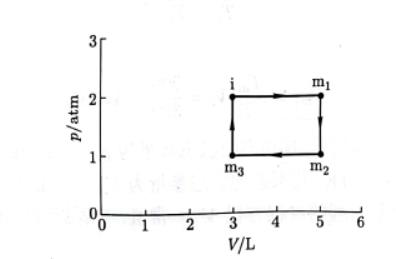
\includegraphics[width=0.4\textwidth]{rectangle_circle.png}
  \caption{题 4.21 矩形循环 p-V 图}
  \label{fig:rectangle_circle_v}
\end{figure}

\textbf{(2) 循环净功}

循环过程中气体对外界所做的净功等于 $p$-$V$ 图上闭合曲线所围面积。仅等压过程做功，等体过程做功为零：
\begin{align*}
W'&=\int_{\mathrm{i}}^{\mathrm{m}_1}p\,\mathrm{d}V+\int_{\mathrm{m}_2}^{\mathrm{m}_3}p\,\mathrm{d}V\\
&=p_{\mathrm{i}}(V_{\mathrm{m}_1}-V_{\mathrm{i}})+p_{\mathrm{m}_2}(V_{\mathrm{m}_3}-V_{\mathrm{m}_2})\\
&=2\times 10^{5}\times(5-3)\times 10^{-3}+1\times 10^{5}\times(3-5)\times 10^{-3}\\
&=400-200=200\ \mathrm{J}.
\end{align*}
故
\[
\boxed{W'=200\ \mathrm{J}}.
\]

\textbf{(3) 循环效率}

因为氧气为双原子分子气体，其定体摩尔热容 $C_{V,\mathrm{m}}=\dfrac{5}{2}R$，定压摩尔热容 $C_{p,\mathrm{m}}=\dfrac{7}{2}R$。

各过程的热量交换：

\textit{过程 $\mathrm{i}\to\mathrm{m}_1$（等压吸热）}：
\[
Q_{1}=C_{p}(T_{\mathrm{m}_1}-T_{\mathrm{i}})
=\nu C_{p,\mathrm{m}}(T_{\mathrm{m}_1}-T_{\mathrm{i}})
=\frac{7}{2}\nu R(T_{\mathrm{m}_1}-T_{\mathrm{i}})
=\frac{7}{2}(p_{\mathrm{m}_1}V_{\mathrm{m}_1}-p_{\mathrm{i}}V_{\mathrm{i}})
=\frac{7}{2}\times(2\times 10^{5}\times 5\times 10^{-3}-2\times 10^{5}\times 3\times 10^{-3})
=1400\ \mathrm{J}.
\]

\textit{过程 $\mathrm{m}_1\to\mathrm{m}_2$（等体放热）}：
\[
Q_{2}=C_{V}(T_{\mathrm{m}_2}-T_{\mathrm{m}_1})
=\nu C_{V,\mathrm{m}}(250-500)
=\frac{5}{2}\nu R(-250)<0.
\]

\textit{过程 $\mathrm{m}_2\to\mathrm{m}_3$（等压放热）}：
\[
Q_{3}=C_{p}(T_{\mathrm{m}_3}-T_{\mathrm{m}_2})
=\nu C_{p,\mathrm{m}}(150-250)
=\frac{7}{2}\nu R(-100)<0.
\]

\textit{过程 $\mathrm{m}_3\to\mathrm{i}$（等体吸热）}：
\[
Q_{4}=C_{V}(T_{\mathrm{i}}-T_{\mathrm{m}_3})
=\nu C_{V,\mathrm{m}}(T_{\mathrm{i}}-T_{\mathrm{m}_3})
=\frac{5}{2}(p_{\mathrm{i}}V_{\mathrm{i}}-p_{\mathrm{m}_3}V_{\mathrm{m}_3})
=\frac{5}{2}\times(2\times 10^{5}\times 3\times 10^{-3}-1\times 10^{5}\times 3\times 10^{-3})
=750\ \mathrm{J}.
\]

循环中系统吸收的总热量为
\[
Q_{\text{吸}}=Q_{1}+Q_{4}=1400+750=2150\ \mathrm{J}.
\]

于是该循环的效率为
\[
\eta=\frac{W'}{Q_{\text{吸}}}=\frac{200}{2150}\approx 9.3\%.
\]
即
\[
\boxed{\eta\approx 9.3\%}.
\]

\subsubsection{题 4.25（等压-等体-绝热循环效率）}

\textbf{题目}：设有一以理想气体为工作物质的热机循环，如图所示，由等压过程 $C\to A$、等体过程 $A\to B$ 和绝热过程 $B\to C$ 所组成。若已知 $p_A,p_B,V_A,V_C$ 和绝热指数 $\gamma$，试证明此热机的循环效率为
\[
\eta=1-\gamma\,\frac{(V_C/V_A)-1}{(p_B/p_A)-1}.
\]

% [插图：题 4.25 等压-等体-绝热循环 p-V 图]
\begin{figure}[htbp]
  \centering
  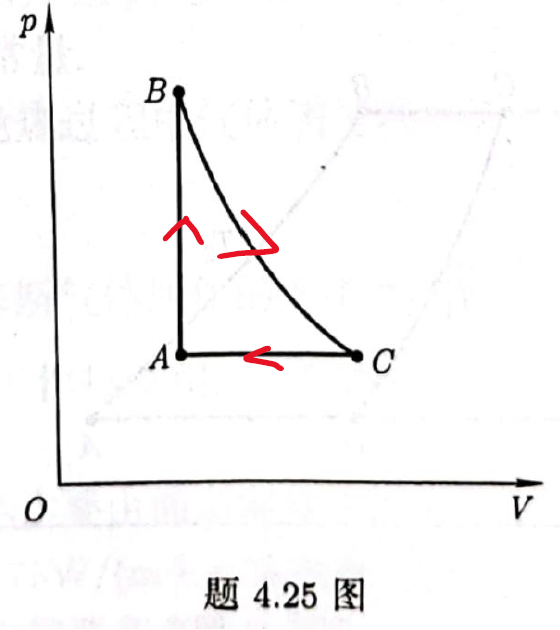
\includegraphics[width=0.4\textwidth]{4_25.png}
  \caption{题 4.25 等压-等体-绝热循环 p-V 图}
  \label{fig:4_25}
\end{figure}

\textbf{证明}：

依题意，理想气体在 $A\to B$ 的等体过程中吸热，在 $C\to A$ 的等压过程中放热，于是有
\[
Q_1=C_V(T_B-T_A),\qquad Q'_2=C_p(T_C-T_A).
\]

由循环效率的定义
\[
\eta=1-\frac{Q'_2}{Q_1}
=1-\frac{C_p(T_C-T_A)}{C_V(T_B-T_A)}
=1-\gamma\,\frac{T_C/T_A-1}{T_B/T_A-1}.
\tag{1}
\]

对 $A\to B$ 的等体过程，由理想气体状态方程 $pV=\nu RT$ 及 $V=\text{常量}$，得
\[
\frac{T_B}{T_A}=\frac{p_B}{p_A}.
\]

对 $C\to A$ 的等压过程，由 $p=\text{常量}$，得
\[
\frac{T_C}{T_A}=\frac{V_C}{V_A}.
\]

将以上两式代入 (1) 式，即得
\[
\boxed{\eta=1-\gamma\,\frac{(V_C/V_A)-1}{(p_B/p_A)-1}}.
\]

\subsubsection{题 4.26（奥托循环效率）}

\textbf{题目}：四冲程汽油机的工作循环（奥托循环或定容加热循环）如图所示。工作开始时，一定量的雾状汽油和空气的混合气体由状态 $V_1,T_A$ 绝热压缩到状态 $V_2,T_B$，达到可燃点；此刻，火花塞放出电火花，点燃气体，经等体加热至状态 $V_2,T_C$；燃烧形成的高温气体经绝热膨胀至状态 $V_1,T_D$；后经等体放热使气体恢复到初始状态 $V_1,T_A$。若工作气体可近似为理想气体，试确定该工作循环的效率。

% [插图：题 4.26 奥托循环 p-V 图]
\begin{figure}[htbp]
  \centering
  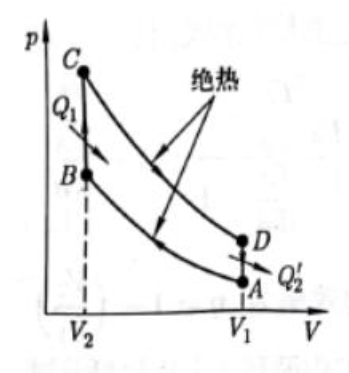
\includegraphics[width=0.4\textwidth]{4_26.png}
  \caption{题 4.26 奥托循环 p-V 图}
  \label{fig:4_26}
\end{figure}

\textbf{解答}：

依题意，奥托循环由两个绝热过程 $A\to B$、$C\to D$ 和两个等体过程 $B\to C$、$D\to A$ 组成，其中 $B\to C$ 为等体升温吸热过程，$D\to A$ 为等体降温放热过程。

在一个循环中，工作物质吸收的热量为
\[
Q_1=C_V(T_C-T_B),
\]
放出的热量为
\[
Q'_2=C_V(T_D-T_A).
\]

由循环效率的定义
\[
\eta=\frac{W'}{Q_1}=\frac{Q_1-Q'_2}{Q_1}
=1-\frac{Q'_2}{Q_1}
=1-\frac{T_D-T_A}{T_C-T_B}
=1-\frac{T_A}{T_B}\,\frac{T_D/T_A-1}{T_C/T_B-1}.
\tag{1}
\]

因为 $A\to B$ 为绝热过程，工作物质可近似为理想气体，由绝热过程方程 $TV^{\gamma-1}=\text{常量}$，得
\[
T_A V_A^{\gamma-1}=T_B V_B^{\gamma-1},
\qquad\Longrightarrow\qquad
\frac{T_A}{T_B}=\left(\frac{V_B}{V_A}\right)^{\gamma-1}
=\left(\frac{V_2}{V_1}\right)^{\gamma-1}.
\tag{2}
\]

同理，对 $C\to D$ 的绝热过程，有
\[
\frac{T_D}{T_C}=\left(\frac{V_C}{V_D}\right)^{\gamma-1}
=\left(\frac{V_2}{V_1}\right)^{\gamma-1}.
\tag{3}
\]

比较 (2) 式和 (3) 式，得
\[
\frac{T_A}{T_B}=\frac{T_D}{T_C},
\qquad\Longrightarrow\qquad
\frac{T_D}{T_A}=\frac{T_C}{T_B}.
\tag{4}
\]

将 (2) 式和 (4) 式代入 (1) 式，得
\[
\eta=1-\frac{T_A}{T_B}\,\frac{T_C/T_B-1}{T_C/T_B-1}
=1-\frac{T_A}{T_B}
=1-\left(\frac{V_2}{V_1}\right)^{\gamma-1}.
\]

记绝热压缩比 $r=\dfrac{V_1}{V_2}$，则
\[
\boxed{\eta=1-\frac{1}{r^{\gamma-1}}=1-\frac{T_A}{T_B}}.
\]

\subsubsection{题 4.32（克劳修斯气体）}

\textbf{题目}：$1\ \mathrm{mol}$ 克劳修斯气体状态方程 $p(V_m-b)=RT$，摩尔内能 $U_m=C_{V,m}T+U_0$，$C_{V,m},U_0$ 为常量。
(1) 证明准静态绝热方程 $p(V_m-b)^{\gamma}=\text{常量}$；
(2) 证明该气体卡诺循环效率仍为 $\eta=1-T_2/T_1$。

\begin{thoughts}
  绝热状态下$Q=0$，所以考虑$$dU = -pdV = -\frac{RT}{V_m-b}dV_m = C_{V,m}dT$$，然后用迈耶关系代换即可，卡诺循环的效率和之前求法相同，卡诺热机指的是由两个等温两个绝热过程组成的可逆热机
\end{thoughts}

\textbf{证明}：

(1) 由状态方程 $p(V_m-b)=RT$ 微分得
\[
p\,\mathrm{d}V_m+(V_m-b)\,\mathrm{d}p=R\,\mathrm{d}T
\]

绝热过程 $\mathrm{d}Q=0$，故 $\mathrm{d}U=-p\,\mathrm{d}V_m$，即
\[
C_{V,m}\,\mathrm{d}T=-p\,\mathrm{d}V_m
=-\frac{RT}{V_m-b}\,\mathrm{d}V_m
\]

分离变量：
\[
\frac{\mathrm{d}T}{T}=-\frac{R}{C_{V,m}}\frac{\mathrm{d}V_m}{V_m-b}
\]

积分并利用 $\gamma=\dfrac{C_{p,m}}{C_{V,m}}$，$\dfrac{R}{C_{V,m}}=\gamma-1$，得
\[
\boxed{T(V_m-b)^{\gamma-1}=\text{常量}}
\quad\text{或}\quad
\boxed{p(V_m-b)^{\gamma}=\text{常量}}
\]

(2) 卡诺循环中，等温吸热与放热：
\[
Q_1=RT_1\ln\frac{V_{m,B}-b}{V_{m,A}-b},\qquad
Q'_2=RT_2\ln\frac{V_{m,C}-b}{V_{m,D}-b}
\]

由 (1) 中绝热方程及 $T_B=T_A=T_1$，$T_C=T_D=T_2$，可证
\[
\frac{V_{m,B}-b}{V_{m,C}-b}=\frac{V_{m,A}-b}{V_{m,D}-b}
\]

于是
\[
\boxed{\eta=1-\frac{Q'_2}{Q_1}=1-\frac{T_2}{T_1}}
\]

% [插图：克劳修斯气体卡诺循环 p-V 图]
\begin{figure}[htbp]
  \centering
  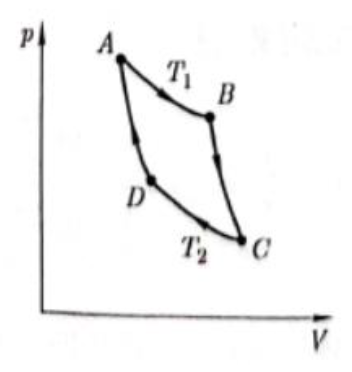
\includegraphics[width=0.4\textwidth]{4_32.png}
  \caption{克劳修斯气体卡诺循环 p-V 图}
  \label{fig:4_32}
\end{figure}



\subsubsection{题 4.33（热泵供暖）}

\textbf{题目}：制冷机作热泵用，室外 $-5^{\circ}\mathrm{C}$，室内保持 $20^{\circ}\mathrm{C}$。
(1) 房间向室外散热主要由面积 $5\ \mathrm{m}^2$、厚 $2\ \mathrm{mm}$ 的玻璃引起，热导率 $\kappa=0.75\ \mathrm{W/(m\cdot K)}$，电费 $0.5$ 元/度。求空调一天工作 $12\ \mathrm{h}$ 至少花多少电费。
(2) 若换为厚 $2\ \mathrm{mm}$、中间有 $0.5\ \mathrm{mm}$ 空气夹层的双层玻璃（空气 $\kappa=0.025\ \mathrm{W/(m\cdot K)}$），求可节省的电费。

\begin{thoughts}
  主要是利用傅里叶公式，单位面积热导和温度梯度成正比\\
  注意到需要设置两个温差变量，利用温差和列出等式，此外空气夹层不储热，所以有热导等式，可解出两端温差，进而求出热导，然后使用制冷机的最大效率等式，解出压缩机功率
\end{thoughts}

\textbf{解答}：

\textbf{(1) 单层玻璃情况下的最小电费计算}

解：依题意，为使室内温度保持不变，则空调在室内放热的功率应该与房间散热的功率相同。记为得到该功率 $Q'_1$ 需要消耗的电功率为 $P$，则由室外（低温热源）吸收并传递到室内（高温热源）的热量为 $Q'_1 - P$。由致冷机的致冷系数的定义知：
\begin{equation}
\varepsilon = \frac{Q'_1 - P}{P} \tag{1}
\end{equation}
于是有：
\begin{equation}
P = \frac{Q'_1}{1+\varepsilon} \tag{2}
\end{equation}
显然，为使花费最少，即使 $P$ 最小，则应该要求致冷系数 $\varepsilon$ 取其可能的最大值。

由热机和致冷机的工作原理知，工作在温度为 $T_1$ 的高温热源和温度为 $T_2$ 的低温热源之间的所有致冷机中，致冷系数的最大值（即卡诺致冷机的致冷系数）为：
\begin{equation}
\varepsilon_{\max} = \varepsilon_C = \frac{T_2}{T_1 - T_2} \tag{3}
\end{equation}
于是有最小输入功率：
\begin{equation}
P_{\min} = \frac{Q'_1}{1+\varepsilon_{\max}} = \frac{T_1 - T_2}{T_1} Q'_1 \tag{4}
\end{equation}
记致冷机 $1$ 天工作的时间为 $t$，工作电费单价为 $c$，工作 $1$ 天需花费的电费为 $C$，则：
\begin{equation}
C_{\min} = P_{\min} t c = \frac{T_1 - T_2}{T_1} Q'_1 t c \tag{5}
\end{equation}

依题意，上述电功率就是玻璃通过热传导的方式散热的功率。由热传导规律知，温差为 $\Delta T$、厚度为 $l$、面积为 $S$、热导率为 $\kappa$ 的导热层传热的功率（散失速率）为：
\begin{equation*}
H = -\kappa \frac{\Delta T}{l} S
\end{equation*}
即有：
\begin{equation}
Q'_1 = -\kappa \frac{\Delta T}{l} S \tag{6}
\end{equation}
于是有：
\begin{equation}
C_{\min}^{(1)} = \frac{T_1 - T_2}{T_1} \left( -\kappa \frac{\Delta T}{l} S \right) t c = \frac{(T_1 - T_2)^2}{T_1 l} S \kappa t c \tag{7}
\end{equation}

将已知数据：
\begin{itemize}
    \item 室内温度 $T_1 = 20 + 273.15 = 293.15\ \mathrm{K}$
    \item 室外温度 $T_2 = -5 + 273.15 = 268.15\ \mathrm{K}$
    \item 温差 $\Delta T = T_2 - T_1 = -25\ \mathrm{K}$
    \item 玻璃厚度 $l = 2 \times 10^{-3}\ \mathrm{m}$
    \item 散热面积 $S = 5\ \mathrm{m}^2$
    \item 玻璃热导率 $\kappa = 0.75\ \mathrm{W/(m\cdot K)} = 0.75 \times 10^{-3}\ \mathrm{kW/(m\cdot K)}$
    \item 工作时间 $t = 12\ \mathrm{h}$
    \item 电费单价 $c = 0.5\ \text{元}/(\mathrm{kW\cdot h})$
\end{itemize}
代入式 (7) ，则得单层玻璃一天的最小电费为：
\begin{align*}
C_{\min}^{(1)} &= \frac{(T_1 - T_2)^2}{T_1 l} S \kappa t c \\
&= \frac{(293.15 - 268.15)^2}{293.15 \times (2 \times 10^{-3})} \times 5 \times (0.75 \times 10^{-3}) \times 12 \times 0.5 \\
&= 23.99 \approx 24\ \text{元}
\end{align*}

\vspace{1em}
\textbf{(2) 双层玻璃情况下的电费及节省电费计算}

依题意，记单层玻璃的厚度为 $l_1$，两层玻璃之间的空气层的厚度为 $l_2$，玻璃层和其间空气层的面积为 $S$。
设玻璃外表面与内表面之间的温度差为 $\Delta T_G$（双层玻璃中，两层玻璃各贡献一次温差），内层玻璃外表面与外层玻璃内表面之间的温度差（即空气层两端的温差）为 $\Delta T_A$。玻璃和空气层的热导率分别为 $\kappa_1, \kappa_2$。

在稳定传热的情况下，各层的热传导功率相等，有：
\begin{equation}
Q'_1 = -\kappa_1 \frac{\Delta T_G}{l_1} S = -\kappa_2 \frac{\Delta T_A}{l_2} S \tag{8}
\end{equation}
又依题意，系统内外总温差满足：
\begin{equation}
2\Delta T_G + \Delta T_A = T_2 - T_1 = -25\ \mathrm{K} \tag{9}
\end{equation}

将式 (8) 和 (9) 联立，可得：
\begin{equation*}
\kappa_1 \frac{\Delta T_G}{l_1} = \kappa_2 \frac{\Delta T_A}{l_2} = \kappa_2 \frac{-25 - 2\Delta T_G}{l_2} = -\frac{25\kappa_2}{l_2} - \frac{2\kappa_2\Delta T_G}{l_2}
\end{equation*}
整理得：
\begin{equation*}
\Delta T_G \left( \frac{\kappa_1}{l_1} + \frac{2\kappa_2}{l_2} \right) = -\frac{25\kappa_2}{l_2}
\end{equation*}
即：
\begin{equation*}
\Delta T_G = \frac{-\dfrac{25\kappa_2}{l_2}}{\dfrac{\kappa_1}{l_1} + \dfrac{2\kappa_2}{l_2}}
\end{equation*}

那么，双层玻璃的传热功率 $Q'_1$ 为：
\begin{equation}
Q'_1 = -\kappa_1 \frac{\Delta T_G}{l_1} S = \frac{25\kappa_1\kappa_2}{l_2\kappa_1 + 2l_1\kappa_2} S \tag{10}
\end{equation}

将式 (10) 代入式 (5)，则得双层玻璃情况下的最小电费为：
\begin{equation}
C_{\min}^{(2)} = \frac{T_1 - T_2}{T_1} \frac{25\kappa_1\kappa_2}{l_2\kappa_1 + 2l_1\kappa_2} S t c \tag{11}
\end{equation}

将已知数据：
\begin{itemize}
    \item $T_1 = 293.15\ \mathrm{K}$，$T_2 = 268.15\ \mathrm{K}$
    \item 玻璃厚度 $l_1 = 2 \times 10^{-3}\ \mathrm{m}$
    \item 空气层厚度 $l_2 = 0.5\ \mathrm{mm} = 5 \times 10^{-4}\ \mathrm{m}$
    \item 玻璃热导率 $\kappa_1 = 0.75 \times 10^{-3}\ \mathrm{kW/(m\cdot K)}$
    \item 空气热导率 $\kappa_2 = 0.025 \times 10^{-3}\ \mathrm{kW/(m\cdot K)}$
    \item $S = 5\ \mathrm{m}^2$，$t = 12\ \mathrm{h}$，$c = 0.5\ \text{元}/(\mathrm{kW\cdot h})$
\end{itemize}
代入式 (11)，则得：
\begin{align*}
C_{\min}^{(2)} &= \frac{25}{293.15} \times \frac{25 \times (0.75 \times 10^{-3}) \times (0.025 \times 10^{-3})}{(0.5 \times 10^{-3}) \times (0.75 \times 10^{-3}) + 2 \times (2 \times 10^{-3}) \times (0.025 \times 10^{-3})} \times 5 \times 12 \times 0.5 \\
&= 2.52\ \text{元}
\end{align*}

那么，一天可节省的电费为：
\begin{equation*}
\Delta C_{\min} = C_{\min}^{(1)} - C_{\min}^{(2)} = 23.99 - 2.52 = 21.47 \approx 21\ \text{元}
\end{equation*}

所以，改用所选的“双层玻璃”后，该空调在 $1$ 天仍工作 $12$ 小时的情况下可以节省的电费大约为 $21$ 元。
% ============================================================

\newpage
\section{第五章：热力学第二定律}
% ============================================================

\subsection{可逆过程与不可逆过程}

\subsubsection{基本定义}

\paragraph{热力学过程}
热力学系统随时间变化的任意过程。

\paragraph{准静态过程}
每一时刻处于平衡态的热力学过程。

\paragraph{可逆过程}
不包含任何耗散效应的准静态过程。

\paragraph{耗散效应}
存在摩擦、粘性扰动、磁滞、电阻等消耗功或潜在作功能力的损失。

\paragraph{可逆过程与不可逆过程的定义}
一个系统由某一状态出发，经过某一过程达到另一个状态，如果存在另一个过程使得系统和外界都完全复原（即系统恢复到原来的状态，同时消除对外界的一切影响），则原来的过程称为\textbf{可逆过程}。反之，如果用任何方式都不可能使系统和外界都完全复原，则称原来的过程为\textbf{不可逆过程}。

\begin{itemize}[leftmargin=2em]
  \item \textbf{不可逆过程举例}：气体向真空的自由膨胀（$i\to f$：$\Delta U=0,\,Q=0,\,W=0$。不消耗功，气体再也回复不到初始状态）。
  \item \textbf{自发过程一定不可逆}。
  \item \textbf{热（质、粘性）扩散也是不可逆过程}：高温$\to$低温（自发）；低温$\to$高温（必须外力影响）。
  \item \textbf{焦耳--汤姆孙效应}是一个典型的不可逆过程。
\end{itemize}

在热力学系统中，仅没有耗散效应的准静态过程才是可逆过程。实际过程（如：非准静态过程、有耗散的过程、相不平衡过程等）都是不可逆过程。\textbf{可逆过程只是理想过程，或近似过程}。


% ============================================================
\subsection{热力学循环及效率}
% ============================================================

若循环的每一阶段都是准静态过程，则此循环可用 $p$--$V$ 图上的一条闭合曲线表示。箭头表示过程进行的方向。工质在整个循环过程中对外作的净功等于曲线所包围的面积。

\begin{itemize}[leftmargin=2em]
  \item 沿顺时针方向进行的循环称为\textbf{正循环}。
  \item 沿反时针方向进行的循环称为\textbf{逆循环}。
\end{itemize}

\paragraph{正循环的特征}
一定质量的工质在一次循环过程中要从高温热源吸热 $Q_1$，对外作净功 $|W|$，又向低温热源放出热量 $Q_2$。而工质回到初态，\textbf{内能不变}。$Q_1$、$Q_2$、$|W|$ 均表示数值大小。工质经一个循环后则有：
\[
|W|=Q_1-Q_2
\]
实用上，用\textbf{效率}表示热机的效能，以 $\eta$ 表示：
\[
\boxed{\eta=\frac{|W|}{Q_1}}
\]

\paragraph{逆循环的特征（制冷循环）}
一定质量的工质在一次循环过程中要从低温热源吸热 $|Q_2|$，外界对系统作净功 $|W|$，又向高温热源放出热量 $|Q_1|$。而工质回到初态，\textbf{内能不变}。工质经一个循环后则有：
\[
|W|=|Q_1|-|Q_2|
\]
实用上，用\textbf{制冷系数}表示制冷机的效能，以 $\varepsilon$ 表示：
\[
\boxed{\varepsilon=\frac{|Q_2|}{|W|}}
\]

% [插图：正循环与逆循环 p-V 图，标注方向与面积]
\begin{figure}[htbp]
  \centering
  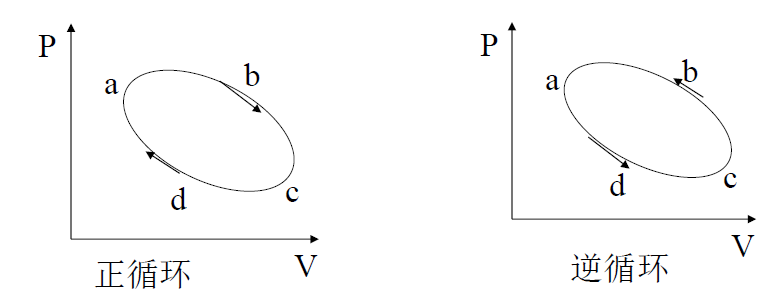
\includegraphics[width=0.7\textwidth]{cycle.png}
  \caption{正循环与逆循环 p-V 图，标注方向与面积}
  \label{fig:cycle_v}
\end{figure}



% ============================================================
\subsection{卡诺循环}
% ============================================================

1824年卡诺（法国工程师 1796--1832）提出了一个能体现热机循环基本特征的理想循环。后人称之为\textbf{卡诺循环}。

\paragraph{卡诺循环的特点}
\begin{enumerate}[leftmargin=2em]
  \item 它由四个准静态过程组成（两个等温、两个绝热）。
  \item 对工作物质没有规定，一般以理想气体为工作物质。
  \item 需要两个热源：高温热源 $T_1$ 和低温热源 $T_2$。
\end{enumerate}

本节讨论以\textbf{理想气体为工质}的正向卡诺循环：

\begin{itemize}[leftmargin=2em]
  \item \textbf{$1\to 2$}：与温度为 $T_1$ 的高温热源接触，$T_1$ 不变，体积由 $V_1$ 膨胀到 $V_2$，从热源 $T_1$ 吸收热量为：
  \[
  Q_1=\nu RT_1\ln\frac{V_2}{V_1}
  \]
  \item \textbf{$2\to 3$}：绝热膨胀，体积由 $V_2$ 变到 $V_3$，吸热为零。
  \item \textbf{$3\to 4$}：与温度为 $T_2$ 的低温热源接触，$T_2$ 不变，体积由 $V_3$ 压缩到 $V_4$，向热源 $T_2$ 放热为：
  \[
  Q_2=\nu RT_2\ln\frac{V_3}{V_4}
  \]
  \item \textbf{$4\to 1$}：绝热压缩，体积由 $V_4$ 变到 $V_1$，吸热为零。
\end{itemize}

在一次循环中，以热力学第一定律，气体对外作净功为：
\[
|W|=Q_1-Q_2
\]

\paragraph{卡诺热机效率}
\[
\eta=\frac{|W|}{Q_1}=\frac{Q_1-Q_2}{Q_1}=1-\frac{Q_2}{Q_1}
=1-\frac{T_2\ln\dfrac{V_3}{V_4}}{T_1\ln\dfrac{V_2}{V_1}}
\]
由第四章绝热过程关系可知：
\[
\frac{V_3}{V_4}=\frac{V_2}{V_1}
\]
所以求得\textbf{卡诺热机的效率}为：
\[
\boxed{\eta=1-\frac{T_2}{T_1}}
\]

\paragraph{总结}
\begin{enumerate}[leftmargin=2em]
  \item 卡诺热机的效率与工作物质无关，只与两个热源的温度有关。$T_2/T_1$ 越小越好，即提高效率的途径是提高高温热源的温度或降低低温热源的温度，而后一种方法是不经济的。
  \item 由于 $T_1=\infty,\,T_2=0$ 都是达不到的，因此卡诺热机的效率总是小于 $1$ 的。
\end{enumerate}

% [插图：卡诺循环 p-V 图与能流图，标注 $Q_1,Q_2,W,T_1,T_2$]
\begin{figure}[htbp]
  \centering
  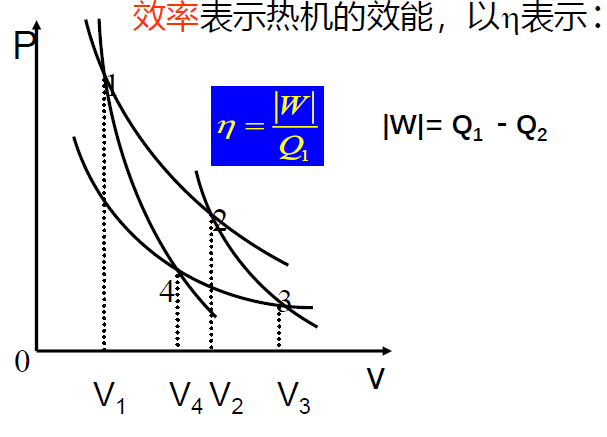
\includegraphics[width=0.45\textwidth]{carnot.png}
  \caption{卡诺循环 p-V 图与能流图，标注 $Q_1,Q_2,W,T_1,T_2$}
  \label{fig:carnot_v}
\end{figure}

% ============================================================
\subsection{热力学第二定律的表述}
% ============================================================

一个热力学过程，除了必须遵守热力学第一定律（即能量守恒）外，人们发现还存在另外一条基本定律——规定热力学过程方向的定律，即\textbf{热力学第二定律}。

\paragraph{（1）克劳修斯表述（Clausius, 1850）}
\textbf{不可能把热量从低温物体传到高温物体而不引起任何其他变化。}

\paragraph{（2）开尔文表述（Kelvin, 1851）}
\textbf{不可能从单一热源吸收热量使之完全转变为功而不产生其他影响。}

或：\textbf{第二类永动机是不可能造成的。}

第二类永动机：从单一热源吸热对外作功但不产生其它任何影响的机械。

\paragraph{两种表述的等价性}
\begin{itemize}[leftmargin=2em]
  \item 若违反开尔文表述，则可将热机与制冷机组合，导致热量自发从低温传向高温，违反克劳修斯表述。
  \item 若违反克劳修斯表述，则可将制冷机与热机组合，实现从单一热源吸热全部变成功，违反开尔文表述。
\end{itemize}

% [插图：两种表述等价性示意图，热机与制冷机组合]

% ============================================================
\subsection{卡诺定理}
% ============================================================

在卡诺循环的基础上，考虑过程的不可逆性以及熵增原理。

\paragraph{卡诺定理}
\begin{enumerate}[leftmargin=2em]
  \item 在相同的高温热源和相同的低温热源之间工作的一切\textbf{可逆热机的效率都相等}，与工作物质无关；
  \item 在相同的高温热源和相同的低温热源之间工作的一切\textbf{不可逆热机的效率} $\eta'$ \textbf{都小于可逆热机的效率} $\eta$。
\end{enumerate}

\[
\boxed{\eta'=1-\frac{Q_2'}{Q_1}\le 1-\frac{T_2}{T_1}=\eta}
\]

\paragraph{卡诺定理证明（一）}
设 A、B 都是可逆热机，一个循环中，它们从高温热源 $T_1$ 处吸热 $Q_{A1},Q_{B1}$，对外作功 $W_A',W_B'$，向低温热源 $T_2$ 放热 $Q_{A2}',Q_{B2}'$。有
\[
\eta_A=\frac{W_A'}{Q_{A1}},\quad \eta_B=\frac{W_B'}{Q_{B1}}
\]
设 $Q_{A1}=Q_{B1}$，由热力学第一定律：
\[
Q_{A1}=W_A'+Q_{A2}',\quad Q_{B1}=W_B'+Q_{B2}'
\]
若 $\eta_A>\eta_B$，则 $W_A'>W_B'$，可得 $Q_{B2}'-Q_{A2}'=W_A'-W_B'>0$。考虑 ``A+B逆'' 组成的系统，$T_1$ 处不变，系统从 $T_2$ 处吸收热量 $Q_{B2}'-Q_{A2}'$ 全部转化为功，违背热力学第二定律。故 $\eta_A>\eta_B$ 不成立。同理 $\eta_A<\eta_B$ 不成立。因此
\[
\eta_A=\eta_B
\]

\paragraph{卡诺定理证明（二）}
假设 A 不可逆、B 可逆，且 $\eta_A>\eta_B$。若 $Q_{A1}=Q_{B1}$，则
\[
Q_{B2}'-Q_{A2}'=W_A'-W_B'>0
\]
使 B 逆向运行即有第二类永动机。故 $\eta_A>\eta_B$ 不成立，即 $\eta_{\mathrm{IR}}\le\eta_{\mathrm{R}}$。

若 $\eta_A=\eta_B$，则 $Q_{B2}'-Q_{A2}'=0$，使 B 逆向运行，则系统 A+B 逆组成可逆机，与 A 不可逆矛盾。所以有 $\eta_{\mathrm{IR}}\neq\eta_{\mathrm{R}}$，综合得：
\[
\boxed{\eta_{\mathrm{IR}}<\eta_{\mathrm{R}}}
\]

\paragraph{卡诺定理应用：非理想气体内能方程}
考虑一个微小的卡诺正循环：AB、CD 为等温线；BC、DA 为绝热线。循环足够小，ABCD 可看成平行四边形。
\begin{itemize}[leftmargin=2em]
  \item 对外做功：$\Delta W'_{\mathrm{total}}=S_{ABCD}=(\Delta p)_V(\Delta V)_T$
  \item 从外吸热（AB 段）：
  \[
  \Delta Q_{AB}=(\Delta U)_T+\Delta W'_{AB}=(\Delta U)_T+S_{ABGH}
  \]
  其中 $p_B=p-(\Delta p)_T$，$S_{ABGH}=\dfrac{1}{2}(\Delta V)_T(p+p_B)=(\Delta V)_T\!\left[p-\dfrac{1}{2}(\Delta p)_T\right]$。
\end{itemize}

代入并整理，令 $\Delta T\to 0$，可得\textbf{内能方程}：
\[
\boxed{\left(\frac{\partial U}{\partial V}\right)_T=T\left(\frac{\partial p}{\partial T}\right)_V-p}
\]
将一般物质内能（和体积的关系）与物质的状态联系起来。若理想气体 $p=\dfrac{\nu RT}{V}$，则
\[
\left(\frac{\partial U}{\partial V}\right)_T=T\frac{\nu R}{V}-p=0
\]


% ============================================================
\subsection{熵及热力学第二定律的统计意义}
% ============================================================

\subsubsection{从有序向无序转化的微观解释}

\begin{enumerate}[leftmargin=2em]
  \item 气体向真空膨胀这一不可逆的自发过程，从统计意义上说是一种从概率较小的状态向概率较大的状态过渡的过程；
  \item 当分子数目越多，分子平均分布的概率就越大，其不可逆性越强；
  \item 根据统计解释，分子平均分布的结果是内部压力处处相等，达到平衡态，即平衡态是系统自发过程的概率最大状态；
  \item 在给定条件下，以系统微观状态数的多寡描述一个系统的无序程度，那么平衡态对应的是无序度最大的状态。
\end{enumerate}

\subsubsection{熵及熵变}

\paragraph{熵的定义}
由系统的\textbf{热温比}沿可逆路径的积分定义的态函数称为系统的\textbf{熵}，记为 $S$，即有
\[
\boxed{\Delta S=S_f-S_i=\int_i^f\frac{\mathrm{d}Q}{T}}
\]
对于无穷小元过程，则有
\[
\mathrm{d}S=\frac{\mathrm{d}Q}{T}
\]
$S$：态函数——总变化量只和初始状态及最终状态有关。

\paragraph{熵的部分性质}
\begin{itemize}[leftmargin=2em]
  \item \textbf{熵是态函数}：$S=S(T,V)$，$S=S(T,p)$（没有外场）。
  \item \textbf{熵是由可逆过程定义的}：从而两状态间的熵变只能通过可逆过程计算。
  \item \textbf{可以通过选取合适的参考点确定系统的熵}：
  \[
  S-S_0=\int_R\frac{\mathrm{d}Q}{T}
  \]
\end{itemize}

\paragraph{数学表述（玻尔兹曼熵公式）}
对于孤立系统：
\[
\boxed{S=k_B\ln\Omega},\qquad \Delta S=k_B\ln\frac{\Omega_f}{\Omega_i}
\]
其中 $f$ 代表 final state；$i$ 代表 initial state。

取对数形式是为了和宏观热力学保持一致。

对于一个封闭系统，如果过程绝热且可逆，由 $\mathrm{d}Q=T\mathrm{d}S$ 得到 $\mathrm{d}S=0$；另外，从微观角度证明了对于一切不可逆过程，整个系统总是朝着熵增加的方向进行。

因而，一个封闭的系统如果和外界没有任何能量交换（即孤立系统），其自发的过程总有：
\[
\boxed{\mathrm{d}S_{\mathrm{iso}}\ge 0}
\]
即对于孤立系统，总有 $\Omega_f\ge\Omega_i$。此即\textbf{热力学第二定律的统计意义}。

\subsubsection{熵定律是统计规律}

宏观过程的不可逆性只是在\textbf{统计意义上的``不可逆''}，并不是绝对的``不可逆''。

自由膨胀：
\[
\Delta S=\nu R\ln\frac{V_f}{V_i}=\nu R\ln 2
\]
统计解释：$\Delta S=k_B\ln(\Omega_f/\Omega_i)$，这里 $\dfrac{\Omega_f}{\Omega_i}=2^N$。

从\textbf{统计规律性}的角度看，自发进行的\textbf{不可逆过程}是由\textbf{概率较小}的状态向\textbf{概率较大}的状态过渡的过程。

由概率较大的宏观状态向概率较小的宏观状态过渡，即不可逆过程的逆过程并不是绝对不可能，只是可能性极小极小而已。

% ============================================================
\subsection{熵变的计算}
% ============================================================

\subsubsection{热力学基本方程}

热力学第一定律：$\mathrm{d}Q=\mathrm{d}U-\mathrm{d}W$

对于可逆过程：$\mathrm{d}Q=T\mathrm{d}S$，$\mathrm{d}W=-p\,\mathrm{d}V$

\[
\mathrm{d}Q=\mathrm{d}U-\mathrm{d}W=\mathrm{d}U+p\,\mathrm{d}V
=\mathrm{d}(U+pV)-V\mathrm{d}p=\mathrm{d}H-V\mathrm{d}p
\]

两式联立则得
\[
\boxed{T\mathrm{d}S=\mathrm{d}U+p\,\mathrm{d}V},\qquad
\boxed{T\mathrm{d}S=\mathrm{d}H-V\mathrm{d}p}
\]
此即\textbf{热力学基本方程}，也常称为 $TdS$ 方程。\textbf{对不可逆过程也成立！}

\subsubsection{可逆过程熵变的计算}

以 $T,V$ 为自变量，$U=U(T,V)$：
\begin{align*}
\mathrm{d}S&=\frac{\mathrm{d}U}{T}+\frac{p}{T}\,\mathrm{d}V
=\frac{1}{T}\!\left[\left(\frac{\partial U}{\partial T}\right)_V\mathrm{d}T
+\left(\frac{\partial U}{\partial V}\right)_T\mathrm{d}V\right]
+\frac{p}{T}\,\mathrm{d}V\\[4pt]
&=\frac{C_V}{T}\,\mathrm{d}T+\frac{1}{T}\!\left[\left(\frac{\partial U}{\partial V}\right)_T+p\right]\mathrm{d}V
=\frac{C_V}{T}\,\mathrm{d}T+\left(\frac{\partial p}{\partial T}\right)_V\mathrm{d}V
\end{align*}

积分得
\[
\Delta S=S_f-S_i=\int_i^f\frac{C_V}{T}\,\mathrm{d}T
+\int_i^f\left(\frac{\partial p}{\partial T}\right)_V\mathrm{d}V
\]

以 $T,p$ 为自变量，$H=H(T,p)$：
\[
\mathrm{d}S=\frac{\mathrm{d}H}{T}-\frac{V}{T}\,\mathrm{d}p
=\frac{C_p}{T}\,\mathrm{d}T-\left(\frac{\partial V}{\partial T}\right)_p\mathrm{d}p
\]
\[
\Delta S=S_f-S_i=\int_i^f\frac{C_p}{T}\,\mathrm{d}T
-\int_i^f\left(\frac{\partial V}{\partial T}\right)_p\mathrm{d}p
\]

\paragraph{焓公式}
\[
\left(\frac{\partial H}{\partial p}\right)_T=-T\left(\frac{\partial V}{\partial T}\right)_p+V
\]

\subsubsection{理想气体熵变的计算}

通过热容和物态方程计算熵。对理想气体：
\[
\left(\frac{\partial p}{\partial T}\right)_V=\frac{\nu R}{V},\qquad
\left(\frac{\partial V}{\partial T}\right)_p=\frac{\nu R}{p}
\]

\paragraph{以 $(T,V)$ 为变量}
\[
S(T,V)=\int_{T_0}^T\frac{C_V}{T}\,\mathrm{d}T+\int_{V_0}^V\frac{\nu R}{V}\,\mathrm{d}V+S_0
=C_V\ln\frac{T}{T_0}+\nu R\ln\frac{V}{V_0}+S_0
\]

\paragraph{以 $(T,p)$ 为变量}
\[
S(T,p)=\int_{T_0}^T\frac{C_p}{T}\,\mathrm{d}T-\int_{p_0}^p\frac{\nu R}{p}\,\mathrm{d}p+S_0
=C_p\ln\frac{T}{T_0}-\nu R\ln\frac{p}{p_0}+S_0
\]

\paragraph{各种可逆过程的熵变}

\begin{itemize}[leftmargin=2em]
  \item \textbf{可逆等温过程}：
  \[
  \Delta S=\nu R\ln\frac{V_f}{V_i}=-\nu R\ln\frac{p_f}{p_i}
  \]
  \item \textbf{可逆等压过程}：
  \[
  \Delta S=C_p\ln\frac{T_f}{T_i}
  \]
  \item \textbf{可逆绝热过程}：
  \[
  \mathrm{d}S=\frac{\mathrm{d}Q}{T}=0
  \]
  \item \textbf{可逆等体过程}：
  \[
  \Delta S=C_V\ln\frac{T_f}{T_i}
  \]
  \item \textbf{可逆多方过程}（$pV^n=\text{常量}$）：
  \[
  \Delta S=C_V\ln\frac{T_f}{T_i}+\nu R\ln\frac{V_f}{V_i}
  =\left[C_V+\frac{\nu R}{1-n}\right]\ln\frac{T_f}{T_i}
  =C_n\ln\frac{T_f}{T_i}
  \]
  其中多方过程热容
  \[
  C_n=\frac{n-\gamma}{n-1}C_V=\frac{C_p-nC_V}{1-n}
  \]
\end{itemize}

不同过程的熵计算公式不同并不表示熵是过程量，而是因为过程的终态不一样。

\paragraph{$T$-$S$ 图上理想气体的多方过程}
对于理想气体的多方过程，前面已经得出：
\begin{enumerate}[leftmargin=2em]
  \item $pV^n=\text{常量}$ 或者 $TV^{n-1}=\text{常量}$
  \item $\Delta S=C_V\ln\dfrac{T_2}{T_1}+\nu R\ln\dfrac{V_2}{V_1}$
  \item $\Delta S=C_n\ln\dfrac{T_2}{T_1}$ 或者 $\mathrm{d}S=C_n\dfrac{\mathrm{d}T}{T}$
\end{enumerate}

进一步求得多方过程曲线的斜率为
\[
\left(\frac{\mathrm{d}T}{\mathrm{d}S}\right)_n=\frac{T}{C_n}
=\frac{T(n-1)(\gamma-1)}{R(n-\gamma)}
\]

特殊过程：
\[
\text{等体：}\left(\frac{\mathrm{d}T}{\mathrm{d}S}\right)_{n=\infty}=\frac{T}{C_V},\quad
\text{等压：}\left(\frac{\mathrm{d}T}{\mathrm{d}S}\right)_{n=0}=\frac{T}{C_p},\quad
\text{等温：}\left(\frac{\mathrm{d}T}{\mathrm{d}S}\right)_{n=1}=0,\quad
\text{绝热：}\left(\frac{\mathrm{d}T}{\mathrm{d}S}\right)_{n=\gamma}=\infty
\]

\subsubsection{不可逆过程的熵变}

\textbf{不能直接沿不可逆路径积分求得，而应采用间接途径。}

\paragraph{方法}
\begin{enumerate}[leftmargin=2em]
  \item 设计一个连接相同的初态和相同的末态的\textbf{可逆路径}，根据态函数的性质，通过计算该可逆过程的熵变求得不可逆过程的熵变。
  \item 给出熵函数的参考点，计算出熵作为\textbf{态函数的形式} $\boldsymbol{S(T,V)}$ 或 $\boldsymbol{S(T,p)}$，然后把初末态的状态参量代入计算出熵变。
\end{enumerate}

\paragraph{例如：自由膨胀过程的熵变}
理想气体由初态 $i$ 自由膨胀到末态 $f$，有 $Q=0,\,W=0,\,T_f=T_i$。

设计一个\textbf{可逆等温过程}连接初末态：
\[
\Delta S=\nu R\ln\frac{V_f}{V_i}=-\nu R\ln\frac{p_f}{p_i}>0
\]

或设计\textbf{可逆绝热过程 + 可逆等体过程}：
\begin{align*}
\text{可逆绝热：}&\;\Delta S=0\\
\text{可逆等体：}&\;\Delta S=C_V\ln\frac{T_f}{T_m}
\end{align*}
利用绝热关系与状态方程，最终同样得到
\[
\boxed{\Delta S_{FE}=\nu R\ln n>0}\qquad(n>1\text{ 为膨胀比})
\]

不论以什么状态参量表示熵，自由膨胀过程中理想气体熵变都是 $\Delta S_{FE}=\nu R\ln n>0$。

% ============================================================
\subsection{熵增加原理}
% ============================================================

一般情况：孤立系统绝热过程的熵变。初态 $i$ 到末态 $f$ 有各种路径，设 $p$-$V$ 图上 $L$ 是讨论的过程（可逆或不可逆），选另一连接 $i$ 和 $f$ 的可逆路径 $L_0$，则 $(L+\text{逆}L_0)$ 构成一个循环。由克劳修斯不等式
\[
\oint\frac{\mathrm{d}Q}{T}=\int_L\frac{\mathrm{d}Q}{T}+\int_{-L_0}\frac{\mathrm{d}Q}{T}\le 0
\quad\Longrightarrow\quad
\int_L\frac{\mathrm{d}Q}{T}\le\int_{L_0}\frac{\mathrm{d}Q}{T}
\]

$i$ 到 $f$ 的过程中熵变为
\[
\Delta S_L=\int_{L_0}\frac{\mathrm{d}Q}{T}\ge\int_L\frac{\mathrm{d}Q}{T}
\]
对绝热过程 $L$ 则有 $\Delta S_{ad}\ge\displaystyle\int_L\dfrac{\mathrm{d}Q}{T}=0$，即
\[
\boxed{\Delta S_{ad}\ge 0}
\]

实例计算和一般计算都表明，在绝热过程中
\[
\boxed{\Delta S\ge 0}
\]

\textbf{热力学系统从一个平衡态经绝热过程到达另一个平衡态，它的熵永不减少。若过程可逆，则其熵不变；若过程不可逆，则其熵增加。}

判断绝热过程是否可逆，实际计算熵变：
\begin{itemize}[leftmargin=2em]
  \item 若 $\Delta S>0$ 则该绝热过程不可逆；
  \item 若 $\Delta S=0$ 则该绝热过程可逆。
\end{itemize}

克劳修斯不等式的另一种表述：
\[
\boxed{T\mathrm{d}S\ge \mathrm{d}Q}\quad(\text{可逆取等号})
\]

\paragraph{讨论}
\begin{itemize}[leftmargin=2em]
  \item \textbf{熵增加原理}；
  \item 孤立系统绝热过程进行方向的判据（时间箭头）：$\Delta S\ge 0$；
  \item 孤立系统热平衡的判据：熵取得极大值，即 $\mathrm{d}S=0$；
  \item 严格地，在内能和体积不变的条件下，对于一切可能的变动来说，平衡态的熵最大，此时 $\mathrm{d}S=0$。
\end{itemize}

\paragraph{题 5.2（讨论）}
欲使一密闭绝热的房间冷却，是否可以将其中的电冰箱的门打开由电冰箱运转而实现？

\textbf{解：}不可以。电冰箱致冷是由工作物质在冷冻室附近（相当于低温热源）汽化带走热量而实现的。当电冰箱门打开后，冷冻室的温度和房间的温度相同，也就是与压缩机内工作物质的温度相同，整体上讲仅有一个热源，不满足热力学第二定律。另一方面，即使考虑一开始冷冻室附近的温度较低，理论上讲存在两个热源，但由冷冻室附近带走的热量和电机工作转化成的热量都释放到房间内，结果会使得房间内比没有打开电冰箱的门时还要热。

% ============================================================
\subsection{习题解答}
% ============================================================

\subsubsection{题 5.3}

\textbf{题目}：热机在工作循环中实际与多个热源接触并交换热量。记热机从其中吸收热量的热源的最高温度为 $T_{\max}$，热机在其处放热的热源的最低温度为 $T_{\min}$，试证明该热机的效率不可能超过 $(T_{\max}-T_{\min})/T_{\max}$。

\begin{thoughts}
  可以看成许多个卡诺热机，效率不会超过这个值
\end{thoughts}

\textbf{证明}：对于一个任意的可逆循环，可用若干绝热线将可逆循环所包含的面积划分为若干部分。记划分完整的可逆循环绝热线的条数为 $N$，则每两条这样引入的相邻的绝热线与其间的原循环曲线上的曲线段构成一个可逆卡诺循环。

考察从左到右算起来第 $i$ 条绝热线与第 $i+1$ 条绝热线所夹区域中各种能量之间的关系。由于上述第 $i$ 条绝热线与第 $i+1$ 条绝热线之间的局部循环可以视为卡诺循环，所吸收的热量 $\Delta Q_{1i}$ 与放出的热量 $\Delta Q_{2i}$ 之间满足
\[
\frac{\Delta Q_{1i}}{\Delta Q_{2i}}=\frac{T_{1i}}{T_{2i}}
\]
其中 $T_{1i}$ 是局部循环中高温热源的温度，$T_{2i}$ 是其低温热源的温度。

记 $T_{\max}$ 为整个循环中的最高温度，$T_{\min}$ 为其最低温度，则一定满足
\[
T_{1i}\le T_{\max},\qquad T_{2i}\ge T_{\min}
\]

该局部循环对外所做的功 $\Delta W_i'$ 与所吸收的热量 $\Delta Q_{1i}$ 的比值为
\[
\frac{\Delta W_i'}{\Delta Q_{1i}}
=\frac{\Delta Q_{1i}-\Delta Q_{2i}}{\Delta Q_{1i}}
=1-\frac{T_{2i}}{T_{1i}}
\le 1-\frac{T_{\min}}{T_{\max}}
\]

由于该完整的可逆循环的效率为
\[
\eta=\frac{\sum\limits_{i=1}^{N-1}\Delta W_i'}{\sum\limits_{i=1}^{N-1}\Delta Q_{1i}}
=\frac{\sum\limits_{i=1}^{N-1}\left(1-\dfrac{T_{2i}}{T_{1i}}\right)\Delta Q_{1i}}
{\sum\limits_{i=1}^{N-1}\Delta Q_{1i}}
\le\frac{\sum\limits_{i=1}^{N-1}\left(1-\dfrac{T_{\min}}{T_{\max}}\right)\Delta Q_{1i}}
{\sum\limits_{i=1}^{N-1}\Delta Q_{1i}}
=1-\frac{T_{\min}}{T_{\max}}
\]

由于 $\eta=1-\dfrac{T_{\min}}{T_{\max}}$ 是工作在温度为 $T_{\max}$ 的最高温度热源和温度为 $T_{\min}$ 的最低温度热源间的热机的效率，因此该热机的效率不可能超过 $(T_{\max}-T_{\min})/T_{\max}$。
\[
\boxed{\eta\le 1-\frac{T_{\min}}{T_{\max}}}
\]

% [插图：题 5.3 解答图，用绝热线划分循环为若干卡诺循环]
\begin{figure}[htbp]
  \centering
  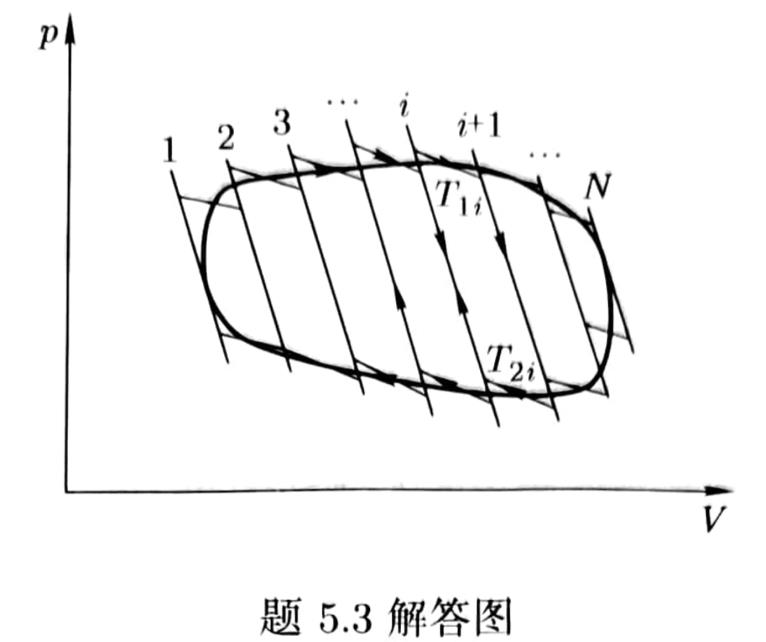
\includegraphics[width=0.45\textwidth]{carnot_separation.png}
  \caption{题 5.4}
  \label{fig:carnot_separation}
\end{figure}

\textbf{题目}：试分别利用热力学第一定律和热力学第二定律证明绝热线与等温线不能相交于两点。

\textbf{证明}：

(1) \textbf{利用热力学第二定律（反证法）}

假设绝热线与等温线可以相交于 $A,B$ 两点。如题 5.4 解答图所示，其中曲线 \raisebox{-1pt}{\textcircled{\scriptsize 1}} 为绝热线，曲线 \raisebox{-1pt}{\textcircled{\scriptsize 2}} 为等温线。显然 $A\to B$ 的等温线与 $B\to A$ 的绝热线形成一个循环。由等温过程和绝热过程的特征知，在该循环过程中，工作物质在 $A\to B$ 的等温变化阶段吸收热量，整个过程结束后，工作物质对外界做曲线包含面积所示数值的功。

这就是说，系统可以由单一热源吸收热量，并且全部转化为有用功而不引起其他任何变化。这显然与热力学第二定律的开尔文表述相矛盾。所以绝热线和等温线可以相交于两点的假设不正确。也就是说，\textbf{绝热线和等温线不能相交于两点}。

(2) \textbf{利用热力学第一定律}

如果等温线在下侧，即题 5.5 解答图中的 $BC$ 和 $CA$ 为绝热线，$AB$ 为等温线，则在此三条线形成的循环过程中，系统向外界做数值为曲边三角形 $\Delta ABC$ 的面积的功，并向外界释放热量，还保持内能不变。这显然与热力学第一定律相矛盾。因此两绝热线相交（于 $C$ 点）是不可能的。

% [插图：题 5.4 解答图，绝热线与等温线相交假设图]
\begin{figure}[htbp]
  \centering
  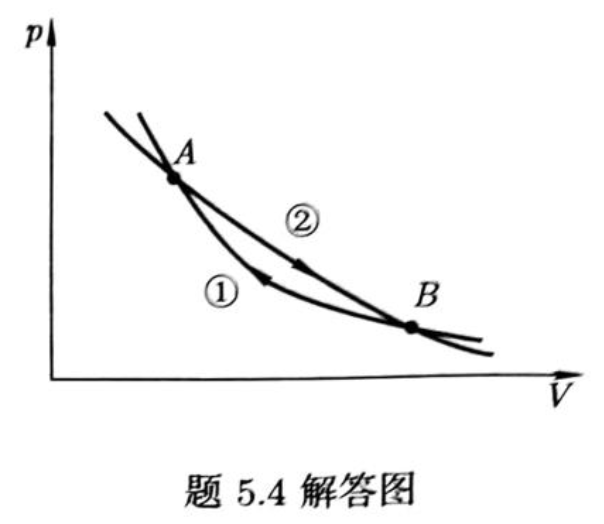
\includegraphics[width=0.4\textwidth]{hypothesis.png}
  \caption{绝热线与等温线相交假设图}
  \label{fig:hypothesis}
\end{figure}

\subsubsection{题 5.5}

\textbf{题目}：试利用热力学第二定律证明两条绝热线不能相交。
\begin{thoughts}
  做一条等温线，证明违背热力学第二定律
\end{thoughts}

\textbf{证明}：

(1) \textbf{反证法}。假设两条绝热线可以相交于一点，如题 5.5 解答图所示，记交点为 $A$。因为绝热线可以与等温线有一个交点，取一条等温线，记等温线与原来的两条绝热线的交点分别为 $B,C$。则 $A,B,C$ 三点间的两段绝热过程和一段等温过程形成一个循环。由绝热过程和等温过程的特征知，在该循环过程中，工作物质在等温过程 $B\to C$ 中从外界吸收热量，对外做曲边三角形 $\Delta ABC$ 的面积所示数值的功。由此知，在这样的循环中，工作物质从单一热源吸收热量并全部转化为有用功而不引起其他任何变化。这显然与热力学第二定律的开尔文表述相矛盾。那么，前述的循环不可能实现。

另一方面，由于等温线与绝热线相交于一点是可以实现的，那么不可能实现的一定是``两条绝热线可以相交于一点''的假设。所以\textbf{两条绝热线不能相交}。

% [插图：题 5.5 解答图，两条绝热线相交假设图]
\begin{figure}[htbp]
  \centering
  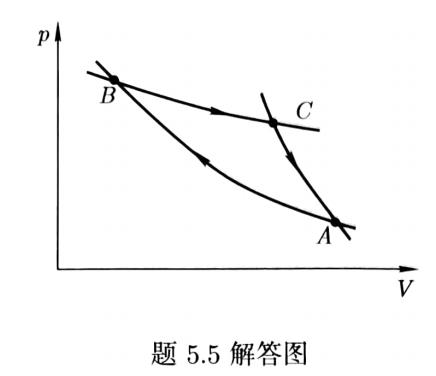
\includegraphics[width=0.4\textwidth]{hypothesis_two.png}
  \caption{两条绝热线相交假设图}
  \label{fig:hypothesis_two}
\end{figure}

\subsubsection{题 5.8}

\textbf{题目}：根据德拜（Debye）定律，金刚石的定容摩尔热容量随温度变化的行为是
\[
C_V=3R\frac{4\pi^4}{5}\left(\frac{T}{\Theta}\right)^3
\]
其中 $\Theta$ 为一确定温度。现有 $1.2\ \mathrm{g}$ 金刚石保持体积一定，温度由 $10\ \mathrm{K}$ 加热到 $350\ \mathrm{K}$，假设形成金刚石的碳的原子量是 $12$，$\Theta=2230\ \mathrm{K}$，试以 $\mathrm{J/K}$ 为单位，确定这些金刚石的熵的改变量。
\begin{thoughts}
  带入熵的定义积分即可
\end{thoughts}

\textbf{解}：依题意，在题设的温度变化范围内，金刚石的体积保持不变，即 $\mathrm{d}V=0$。那么，记这些金刚石的物质的量为 $\nu$。由热力学第一定律得，在其中的一个微小元过程中，金刚石吸收的热量为
\[
\mathrm{d}Q=\mathrm{d}U+\mathrm{d}W=\nu C_{V,m}\,\mathrm{d}T+p\,\mathrm{d}V=\nu C_{V,m}\,\mathrm{d}T
\]

该过程中，金刚石的熵增量为
\[
\Delta S=\int_{T_i}^{T_f}\frac{\mathrm{d}Q}{T}
=\int_{T_i}^{T_f}\frac{\nu C_{V,m}}{T}\,\mathrm{d}T
\tag{1}
\]

将已知条件 $T_f=350\ \mathrm{K}$，$T_i=10\ \mathrm{K}$，$\Theta=2230\ \mathrm{K}$，$\mu=12\times 10^{-3}\ \mathrm{kg/mol}$，$M=1.2\ \mathrm{g}=1.2\times 10^{-3}\ \mathrm{kg}$，$R=8.31\ \mathrm{J/(mol\cdot K)}$ 代入。由
\[
\nu=\frac{M}{\mu},\quad C_{V,m}=3R\frac{4\pi^4}{5}\left(\frac{T}{\Theta}\right)^3
\]
代入 (1) 式，得
\[
\Delta S=3R\frac{4\pi^4}{5}\frac{M}{\mu\Theta^3}\int_{T_i}^{T_f}\frac{T^3}{T}\,\mathrm{d}T
=\frac{4\pi^4 M}{5\mu\Theta^3}R\bigl(T_f^3-T_i^3\bigr)
\tag{2}
\]

\[
\Delta S=\frac{4\times 3.14^4\times(1.2\times 10^{-3})}
{5\times(12\times 10^{-3})\times 2230^3}\times(350^3-10^3)\times 8.31
\approx 0.25\ \mathrm{J/K}
\]

\[
\boxed{\Delta S\approx 0.25\ \mathrm{J/K}}
\]

\subsubsection{题 5.9}

\textbf{题目}：在一绝热材料制成的容器中，温度为 $T_1$、质量为 $m$ 的液体与质量为 $m$、温度为 $T_2$ 的同类液体在保持压强相同的条件下混合，达到平衡态。假设液体的定压比热 $c_p$ 为常量，试确定系统从初态到终态熵的变化量，并证明熵变大于 $0$。

\begin{thoughts}
  首先利用能量守恒求出混合后温度，然后分别计算熵变，使用均值不等式说明熵变大于0
\end{thoughts}

\textbf{解}：两种液体混合达到平衡后，混合液体的温度为 $T_f$。混合过程是在等压条件下进行的。

由能量守恒（热平衡方程）：
\[
mc_p(T_1-T_f)=mc_p(T_f-T_2)\quad\Longrightarrow\quad
T_f=\frac{T_1+T_2}{2}
\]

系统的熵的改变量为两部分液体熵变之和：
\begin{align*}
\Delta S&=\Delta S_1+\Delta S_2
=\int_{T_1}^{T_f}\frac{\mathrm{d}Q_1}{T}+\int_{T_2}^{T_f}\frac{\mathrm{d}Q_2}{T}\\[4pt]
&=\int_{T_1}^{T_f}\frac{mc_p\,\mathrm{d}T}{T}
+\int_{T_2}^{T_f}\frac{mc_p\,\mathrm{d}T}{T}\\[4pt]
&=mc_p\ln\frac{T_f}{T_1}+mc_p\ln\frac{T_f}{T_2}
=mc_p\ln\frac{T_f^2}{T_1T_2}
=mc_p\ln\frac{(T_1+T_2)^2}{4T_1T_2}
\end{align*}

由于
\[
(T_1+T_2)^2-4T_1T_2=(T_1-T_2)^2>0
\quad\Longrightarrow\quad
\frac{(T_1+T_2)^2}{4T_1T_2}>1
\]
故
\[
\boxed{\Delta S=mc_p\ln\frac{(T_1+T_2)^2}{4T_1T_2}>0}
\]

\subsubsection{题 5.11}

\textbf{题目}：$10\ \mathrm{g}\ 20^{\circ}\mathrm{C}$ 的水在定压下变成 $-10^{\circ}\mathrm{C}$ 的冰。假定每克液态水的比热容量保持为 $4.2\ \mathrm{J/(g\cdot K)}$，而且冰的热容量为此值的一半，$0^{\circ}\mathrm{C}$ 的冰的熔解热为 $335\ \mathrm{J/g}$。试确定系统的熵的总变化量。

\begin{thoughts}
  分成三个阶段分别计算即可，降温过程是定压过程，所以$\frac{dQ}{T} = \frac{C_PdT}{T}$，凝结过程是恒温过程，所以用熔解热计算热量即可
\end{thoughts}

\textbf{解}：依题意，该过程是\textbf{降温 $\to$ 凝结 $\to$ 降温}过程。记
\[
m=10\ \mathrm{g},\quad c_1=4.2\ \mathrm{J/(g\cdot K)},\quad
c_2=2.1\ \mathrm{J/(g\cdot K)},\quad l_{\text{凝}}=-335\ \mathrm{J/g}
\]
\[
T_i=20+273.15=293.15\ \mathrm{K},\quad
T_{\text{凝}}=0+273.15=273.15\ \mathrm{K},\quad
T_f=-10+273.15=263.15\ \mathrm{K}
\]

整个过程的熵变为三段之和：
\[
\Delta S=\int\frac{\mathrm{d}Q}{T}
=\int_{T_i}^{T_{\text{凝}}}\frac{mc_1\,\mathrm{d}T}{T}
+\frac{ml_{\text{凝}}}{T_{\text{凝}}}
+\int_{T_{\text{凝}}}^{T_f}\frac{mc_2\,\mathrm{d}T}{T}
\]

\[
\Delta S=mc_1\ln\frac{T_{\text{凝}}}{T_i}
+\frac{ml_{\text{凝}}}{T_{\text{凝}}}
+mc_2\ln\frac{T_f}{T_{\text{凝}}}
\]

代入数值：
\[
\Delta S=10\times 4.2\times\ln\frac{273.15}{293.15}
+\frac{10\times(-335)}{273.15}
+10\times 2.1\times\ln\frac{263.15}{273.15}
\approx -2.97-12.26-0.78=-16.01\ \mathrm{J/K}
\]

\[
\boxed{\Delta S\approx -16\ \mathrm{J/K}}
\]
（理解这个过程的物理情景很重要：系统向外放热，熵减少。）

\subsubsection{题 5.12}

\textbf{题目}：把 $36\ \mathrm{g}\ 20^{\circ}\mathrm{C}$ 的水，在一定的大气压强下变成 $250^{\circ}\mathrm{C}$ 的水蒸气。假定每克液态水的热容量保持为 $4.2\ \mathrm{J/(g\cdot K)}$，而且 $100^{\circ}\mathrm{C}$ 的蒸汽的潜热为 $2260\ \mathrm{J/g}$。如果蒸汽的定压摩尔热容量 $C_{p,\mathrm{m}}$ 与温度的关系为 $C_{p,\mathrm{m}}/R=a+bT+cT^2$，其中 $a=3.634,\ b=1.195\times 10^{-3}\ \mathrm{K}^{-1},\ c=0.135\times 10^{-6}\ \mathrm{K}^{-2}$。试确定系统熵值的总变化量。

\begin{thoughts}
  和上题类似，只不过汽化过程积分计算更复杂
\end{thoughts}

\textbf{解}：依题意，该过程是\textbf{升温 $\to$ 汽化 $\to$ 升温}过程。记
\[
m=36\ \mathrm{g},\quad \mu=18\ \mathrm{g/mol},\quad
T_i=20+273.15=293.15\ \mathrm{K}
\]
\[
T_{\text{汽}}=100+273.15=373.15\ \mathrm{K},\quad
T_f=250+273.15=523.15\ \mathrm{K}
\]
\[
c_p=4.2\ \mathrm{J/(g\cdot K)},\quad l_{\text{汽}}=2260\ \mathrm{J/g}
\]

整个过程的熵变为：
\[
\Delta S=\int\frac{\mathrm{d}Q}{T}
=\int_{T_i}^{T_{\text{汽}}}\frac{mc_p\,\mathrm{d}T}{T}
+\frac{ml_{\text{汽}}}{T_{\text{汽}}}
+\int_{T_{\text{汽}}}^{T_f}\frac{\nu C_{p,\mathrm{m}}\,\mathrm{d}T}{T}
\]

其中 $\nu=m/\mu=2\ \mathrm{mol}$，且
\[
\int\frac{C_{p,\mathrm{m}}}{T}\,\mathrm{d}T
=R\int\left(\frac{a}{T}+b+cT\right)\mathrm{d}T
=R\Bigl[a\ln T+bT+\frac{c}{2}T^2\Bigr]
\]

代入数值：
\begin{align*}
\Delta S&=36\times 4.2\times\ln\frac{373.15}{293.15}
+\frac{36\times 2260}{373.15}
+\frac{36}{18}\times 8.31\times\Bigl[3.634\times\ln\frac{523.15}{373.15}\\
&\qquad+1.195\times 10^{-3}\times(523.15-373.15)
+\tfrac{1}{2}\times 0.135\times 10^{-6}\times(523.15^2-373.15^2)\Bigr]\\[4pt]
&\approx 36.48+218.04+23.54\\[4pt]
&\approx 278.06\ \mathrm{J/K}
\end{align*}

\[
\boxed{\Delta S\approx 278.06\ \mathrm{J/K}}
\]

\subsubsection{题 5.15}

\begin{thoughts}
  需要用微元法计算每一段$dl$的熵变，条件给定$C_P$，核心是温度均匀变化假定，所以实际上是求温度的积分
\end{thoughts}

\textbf{题目}：初始时，均匀细杆的一端的温度为 $T_1$，另一端的温度为 $T_2$。经过一段时间后，杆上温度处处均匀，都为 $(T_1+T_2)/2$。试确定细杆在这两状态间的熵的改变量。

\textbf{解}：设 $T_1>T_2$，以 $T_2$ 端为原点。开始时，杆上 $x\in[0,L]$ 的任意一点处温度为
\[
T_0(x)=T_2+\frac{x}{L}(T_1-T_2)
\]
最后时：
\[
T_f=\frac{1}{2}(T_1+T_2)
\]

记细杆的定压比热容为 $c_p$，质量线密度 $\rho_0=M/L$。在 $x$ 处长度为 $\mathrm{d}x$ 的微元，其质量 $\mathrm{d}M=\rho_0\mathrm{d}x$，温度从 $T_0(x)$ 变到 $T_f$ 时的熵变为
\[
\mathrm{d}(\Delta S)=\int_{T_0(x)}^{T_f}\frac{c_p\,\mathrm{d}M\,\mathrm{d}T}{T}
=c_p\rho_0\mathrm{d}x\ln\frac{T_f}{T_0(x)}
\]

整杆的熵变：
\[
\Delta S=\int_0^L c_p\rho_0\ln\frac{T_f}{T_2+\dfrac{x}{L}(T_1-T_2)}\,\mathrm{d}x
\]

令 $u=T_2+\dfrac{x}{L}(T_1-T_2)$，则 $\mathrm{d}x=\dfrac{L}{T_1-T_2}\mathrm{d}u$，积分得
\[
\Delta S=\frac{Mc_p}{T_1-T_2}\int_{T_2}^{T_1}\ln\frac{T_f}{u}\,\mathrm{d}u
\]

计算积分：
\[
\int\ln\frac{T_f}{u}\,\mathrm{d}u
=u\ln\frac{T_f}{u}+u
\]

代入上下限：
\begin{align*}
\Delta S&=\frac{Mc_p}{T_1-T_2}
\left[u\ln\frac{T_f}{u}+u\right]_{T_2}^{T_1}\\[4pt]
&=\frac{Mc_p}{T_1-T_2}\left[
T_1\ln\frac{T_f}{T_1}+T_1-T_2\ln\frac{T_f}{T_2}-T_2\right]\\[4pt]
&=Mc_p\left[
\frac{T_1\ln T_f-T_1\ln T_1-T_2\ln T_f+T_2\ln T_2}{T_1-T_2}+1\right]\\[4pt]
&=Mc_p\left[1-\ln\frac{T_1+T_2}{2}
-\frac{T_1\ln T_1-T_2\ln T_2}{T_1-T_2}\right]
\end{align*}

整理后：
\[
\boxed{\Delta S=Mc_p\left(1-\ln\frac{T_1+T_2}{2\sqrt{T_1T_2}}\right)}
\quad\text{（或等价形式）}
\]

\subsubsection{题 5.19}

\textbf{题目}：如图，$1\ \mathrm{mol}$ 理想气体氢（$\gamma=1.4$）在状态 $A$ 的参量 $V_A=20\ \mathrm{L},\,T_A=300\ \mathrm{K}$；在状态 $C$ 的参量为 $V_C=40\ \mathrm{L},\,T_C=300\ \mathrm{K}$。图中 $AC$ 为等温线，$AD$ 为绝热线；$AB,DC$ 为等压线，$BC$ 为等体线。试分别由下述三条路径计算 $S_C-S_A$：
(1) $A\to B\to C$；(2) $A\to C$；(3) $A\to D\to C$。

\begin{thoughts}
  由于熵是态函数，熵变与路径无关\\
  从等压-等体过程计算：$dS_P = \frac{C_PdT}{T}$，$dS_V = \frac{C_VdT}{T}$
  从等温过程计算：$dS_T = \frac{dQ}{T} = \frac{PdV}{T} = \frac{RdV}{V}$
  从绝热-等压过程计算：$dS_\gamma = 0$，$dS_P = \frac{C_PdT}{T}$
\end{thoughts}

\textbf{解}：

(1) \textbf{路径 $A\to B\to C$}

$A\to B$ 为等压过程，$B\to C$ 为等体过程。
\[
\frac{T_B}{T_A}=\frac{V_B}{V_A}=\frac{40}{20}=2,\qquad
\frac{T_C}{T_B}=\frac{T_A}{T_B}=\frac{1}{2}
\]
由理想气体的熵公式：
\begin{align*}
S_C-S_A&=(S_B-S_A)+(S_C-S_B)
=C_{p,\mathrm{m}}\ln\frac{T_B}{T_A}+C_{V,\mathrm{m}}\ln\frac{T_C}{T_B}\\[4pt]
&=C_{p,\mathrm{m}}\ln 2+C_{V,\mathrm{m}}\ln\frac{1}{2}
=(C_{p,\mathrm{m}}-C_{V,\mathrm{m}})\ln 2
=R\ln 2
\end{align*}

(2) \textbf{路径 $A\to C$}

$A\to C$ 为等温过程：
\[
S_C-S_A=C_{V,\mathrm{m}}\ln\frac{T_C}{T_A}+R\ln\frac{V_C}{V_A}
=0+R\ln\frac{40}{20}=R\ln 2
\]

(3) \textbf{路径 $A\to D\to C$}

$A\to D$ 为绝热过程，$D\to C$ 为等压过程。对绝热过程：
\[
T_AV_A^{\gamma-1}=T_DV_D^{\gamma-1}
\]
又 $D\to C$ 等压：$\dfrac{V_C}{V_D}=\dfrac{T_C}{T_D}=\dfrac{T_A}{T_D}$。联立并利用 $V_A=20\ \mathrm{L},\,V_C=40\ \mathrm{L}$ 及 $\gamma=1.4$，可得
\[
S_C-S_A=(S_C-S_D)+(S_D-S_A)
=C_{p,\mathrm{m}}\ln\frac{T_C}{T_D}+0
=C_{p,\mathrm{m}}\ln\frac{T_A}{T_D}
\]
利用绝热关系与等压关系化简，最终得
\[
S_C-S_A=R\ln 2
\]

\textbf{结论}：三种路径计算结果相同，
\[
\boxed{S_C-S_A=R\ln 2}
\]
熵是态函数、状态量，与过程无关。

% [插图：题 5.19 p-V 图，标注 A,B,C,D 及各条等值线]
\begin{figure}[htbp]
  \centering
  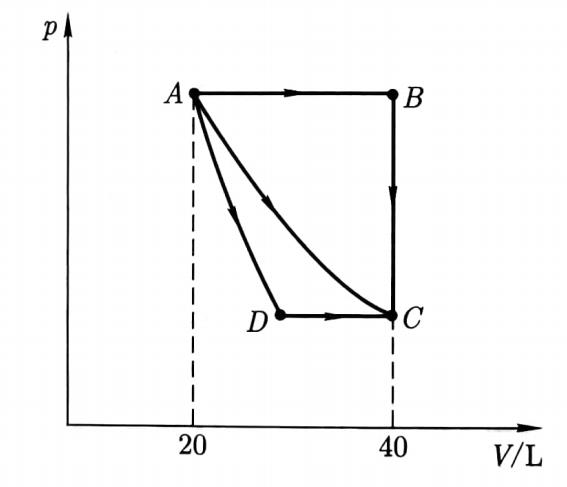
\includegraphics[width=0.4\textwidth]{pV.png}
  \caption{题 5.19 p-V 图}
  \label{fig:pV}
\end{figure}

\subsubsection{题 5.22}

\textbf{题目}：由 $N$ 个微观粒子组成的气体处于容积为 $V_i$ 的容器内，每个粒子都可能处于容器内的任何一处。记容器中的一部分的体积为 $V_p\,(V_p<V_i)$。
\begin{enumerate}[label=(\arabic*), leftmargin=2em]
  \item 试证明，观测到 $N$ 个粒子都处于 $V_p$ 内的概率为 $P_{1p}=\left(\dfrac{V_p}{V_i}\right)^N$；
  \item 试证明，在等温情况下，由 $N$ 个粒子组成的气体系统的体积由 $V_p$ 膨胀到 $V_i$ 后，气体系统的熵的增加量为 $\Delta S=-k_B\ln P_{1p}$，其中 $P_{1p}=\left(\dfrac{V_p}{V_i}\right)^N$，$k_B$ 为玻尔兹曼常量。
\end{enumerate}

\begin{thoughts}
  玻尔兹曼微观熵$$S_B = k_B \ln(\Omega)$$，其余用第二章的统计法计算即可
\end{thoughts}

\textbf{证明}：

(1) 由于微观粒子在 $V_i$ 体积内可等概率地到达任何一处，因此一个粒子到达 $V_p$ 体积内的概率是 $V_p/V_i$。考虑到各个粒子处于 $V_p$ 体积内的事件是相互独立的事件，因此 $N$ 个粒子都处于 $V_p$ 体积内的事件的概率是各粒子处于 $V_p$ 体积内的概率的乘积，即有
\[
P_{1p}=\prod_{i=1}^{N}\frac{V_p}{V_i}=\left(\frac{V_p}{V_i}\right)^N
\]
\[
\boxed{P_{1p}=\left(\frac{V_p}{V_i}\right)^N}
\]

(2) 假设所讨论的气体为理想气体系统，因此包含有 $N$ 个微观粒子的系统的物质的量为 $\nu=N/N_A$，其中 $N_A$ 为阿伏伽德罗常量。

按照理想气体系统的熵的原函数公式，当 $\nu\ \mathrm{mol}$ 气体在等温条件下由体积为 $V_2$ 的态变化到体积为 $V_1$ 的态时，系统的熵增量为
\[
\Delta S=\nu R\ln\frac{V_1}{V_2}
=\nu N_A\frac{R}{N_A}\ln\frac{V_1}{V_2}
=Nk_B\ln\frac{V_1}{V_2}
=k_B\ln\left(\frac{V_1}{V_2}\right)^N
\]

对于题设的体积由 $V_p$ 膨胀到 $V_i$ 的过程，$V_1=V_i,\,V_2=V_p$，并且由第 (1) 问的讨论知，$\left(\dfrac{V_p}{V_i}\right)^N=P_{1p}$，所以
\[
\Delta S=k_B\ln\left(\frac{V_i}{V_p}\right)^N
=-k_B\ln\left(\frac{V_p}{V_i}\right)^N
=-k_B\ln P_{1p}
\]
\[
\boxed{\Delta S=-k_B\ln P_{1p}}
\]

\subsubsection{题 5.23}

\textbf{题目}：一容器内储有由 $1000$ 个微观粒子组成的气体，这些粒子总有机会都处于容积的左半部分，而容器的右半部分完全是空的。试计算，如果观测时间为宇宙寿命长度，即 $150$ 亿年，则在这段时间内，可观测到上述情况的时间为多少秒？并从所得数据出发，说明自由膨胀过程是不可逆过程。

\textbf{解}：记容器的体积为 $V_1$，而左半部分的体积为 $V_2=\dfrac{1}{2}V_1$。所有 $1000$ 个粒子都集中在 $V_2$ 中的概率为
\[
P_{1p}=\left(\frac{V_2}{V_1}\right)^{1000}
=\left(\frac{1}{2}\right)^{1000}
=9.333\times 10^{-302}
\]

显然，这是一个很小的概率。宇宙寿命约 $150$ 亿年，即
\[
t=(150\times 10^8)\times 365\times 24\times 3600
=4.7304\times 10^{17}\ \mathrm{s}
\]

时间内一直观测，则观测到 $1000$ 个粒子都集中在左半部分的时间为
\[
t_{1p}=P_{1p}t=(9.333\times 10^{-302})\times(4.7304\times 10^{17})
\approx 4.415\times 10^{-284}\ \mathrm{s}
\]

附注：根据熵变的概念和本题的计算结果，由 $1000$ 个微观粒子组成的独立系统从原来处于 $V_1$ 体积中转变为处于 $V_2=\dfrac{1}{2}V_1$ 体积中时，系统的熵增量为
\[
\Delta S=k_B\ln\left(\frac{V_2}{V_1}\right)^{1000}
=1000k_B\ln\frac{1}{2}
\approx -9.57\times 10^{-21}\ \mathrm{J/K}
\]
这一熵增量小于零的结果表明这一过程是熵减少过程。按照热力学第二定律，孤立系统不可能出现熵减少过程，但按照本题第 (1) 问的讨论，这种熵减少过程是可能发生的，但发生的概率很小。也就是说，孤立系统中实际不可能发生熵减少过程。

\textbf{结论}：自由膨胀过程是不可逆过程。


\subsubsection{题 5.24}

\textbf{题目}：一热机在温度为 $T_1$ 的物体和温度为 $T_2$ 的热源之间循环工作，使物体的温度下降到 $T_2$ 为止。在该过程中，热机从物体吸收热量 $\Delta Q_1$，对外做功 $W'$，物体的熵的增量为 $\Delta S=S_2-S_1$。试由熵增加原理证明：$W'\le \Delta Q_1+T_2(S_2-S_1)$。

\begin{thoughts}
  熵增加原理$$-\frac{\Delta Q_1-W}{T_2} \leq S_2 - S_1$$
\end{thoughts}

\textbf{证明}：依题意，物体、热源和热机（或者说热机的工作物质）构成一个孤立系统。则系统的总熵变为
\[
\Delta S=\Delta S_{\text{物}}+\Delta S_{\text{源}}+\Delta S_{\text{机}}
\]
热机的工作物质完成一个循环后状态不发生变化，$\Delta S_{\text{机}}=0$。

因为：热源吸收的热机释放出来的热量为 $\Delta Q_{\text{源}}=\Delta Q_1-W'$，且温度保持为 $T_2$，所以热源的熵变：
\[
\Delta S_{\text{源}}=\int\frac{\mathrm{d}Q}{T}=\frac{\Delta Q_{\text{源}}}{T_2}
=\frac{\Delta Q_1-W'}{T_2}
\]

因为：$\Delta S_{\text{物}}=S_2-S_1$

所以：
\[
\Delta S=\Delta S_{\text{物}}+\Delta S_{\text{源}}+\Delta S_{\text{机}}
=(S_2-S_1)+\frac{\Delta Q_1-W'}{T_2}\ge 0
\]

整理得：
\[
\boxed{W'\le \Delta Q_1+T_2(S_2-S_1)}
\]

\subsubsection{题 5.26}

\textbf{题目}：一物体的温度和热源的温度相同，都为 $T_1$。现有一制冷机在此物体和热源之间工作，将物体的温度从 $T_1$ 降到 $T_2$，整个过程中制冷机从物体吸收热量 $Q$，熵的减少量为 $S_1-S_2$。试证明：该过程中外界所提供的功至少为 $W_{\min}=T_1(S_1-S_2)-Q$。

\textbf{证明}：依题意，物体、热源和致冷机构成一个孤立系统，则系统的熵增量为
\[
\Delta S=\Delta S_{\text{物}}+\Delta S_{\text{源}}+\Delta S_{\text{机}}\ge 0
\]
其中 $\Delta S_{\text{机}}=0$（致冷机工作物质完成循环）。

热源吸收的热量等于致冷机放出的热量。即：致冷机从物体吸收的热量 $Q$ 与外界所做的功 $W$ 之和，且 $T_1$ 不变，
\[
\Delta S_{\text{源}}=\int\frac{\mathrm{d}Q}{T}=\frac{Q+W}{T_1}
\]
而物体的熵变：
\[
\Delta S_{\text{物}}=-(S_1-S_2)
\]

代入熵增加原理：
\[
\Delta S=-(S_1-S_2)+\frac{Q+W}{T_1}\ge 0
\quad\Longrightarrow\quad
W\ge T_1(S_1-S_2)-Q
\]

\[
\boxed{W_{\min}=T_1(S_1-S_2)-Q}
\]

\subsubsection{题 5.27}

\textbf{题目}：两个相同的物体的定压热容量 $C_p$ 为常量，温度都为 $T_i$，现使一制冷机在这两个物体之间工作（保持压强不变），把一个物体的温度降为 $T_f$。试证明：该过程所需的最小功为
\[
W_{\min}=C_p\left(\frac{T_i^2}{T_f}+T_f-2T_i\right)
\]

\begin{thoughts}
  用能量守恒定律求出$T'$，然后再用熵增加原理即可
\end{thoughts}

\textbf{证明}：

物体 1：降温物体，$T_i\to T_f$。其熵增量为
\[
\Delta S_1=\int\frac{\mathrm{d}Q}{T}=\int_{T_i}^{T_f}\frac{C_p\,\mathrm{d}T}{T}
=C_p\ln\frac{T_f}{T_i}
\]

物体 2：升温物体，$T_i\to T'$。其熵增量为
\[
\Delta S_2=\int\frac{\mathrm{d}Q}{T}=\int_{T_i}^{T'}\frac{C_p\,\mathrm{d}T}{T}
=C_p\ln\frac{T'}{T_i}
\]

整个孤立系统的熵增量为（制冷机循环 $\Delta S_{\text{机}}=0$）：
\[
\Delta S=\Delta S_1+\Delta S_2+\Delta S_{\text{机}}
=C_p\ln\frac{T_f}{T_i}+C_p\ln\frac{T'}{T_i}
=C_p\ln\frac{T_fT'}{T_i^2}\ge 0
\]

由此得到：
\[
\frac{T_fT'}{T_i^2}\ge 1\quad\Longrightarrow\quad
T'\ge \frac{T_i^2}{T_f}
\]

另一方面，由能量守恒定律，该过程中外界所做的功 $W$ 等于物体 2 吸收的热量与物体 1 放出的热量之差：
\[
W=Q_2-Q_1'=C_p(T'-T_i)-C_p(T_i-T_f)
=C_p(T'+T_f-2T_i)
\]

由于 $T'\ge T_i^2/T_f$，故所需的最小功为
\[
W_{\min}=C_p\left(\frac{T_i^2}{T_f}+T_f-2T_i\right)
\]

\[
\boxed{W_{\min}=C_p\left(\frac{T_i^2}{T_f}+T_f-2T_i\right)}
\]

\subsubsection{题 5.31}

\textbf{题目}：试导出范德瓦尔斯模型下，$\nu\ \mathrm{mol}$ 物质的热力学熵、自由能和自由焓的表达式 $S(T,V)$、$F(T,V)$、$G(T,V)$，画出对应于一确定温度的 $S(V)$、$F(V)$ 和 $G(V)$ 曲线，并与理想气体系统的相应曲线进行比较，说明其间的异同。

\textbf{解}：记范德瓦尔斯气体的内能为温度和体积的函数，即 $U=U(T,V)$。由范德瓦尔斯气体的状态方程
\[
\left(p+\frac{\nu^2 a}{V^2}\right)(V-\nu b)=\nu RT
\]
知
\[
p=\frac{\nu RT}{V-\nu b}-\frac{\nu^2 a}{V^2}
\]

由热力学基本方程与内能方程：
\[
\left(\frac{\partial U}{\partial V}\right)_T
=T\left(\frac{\partial p}{\partial T}\right)_V-p
=\frac{\nu^2 a}{V^2}
\]

于是
\[
U(T,V)=\int C_V\,\mathrm{d}T+\int\frac{\nu^2 a}{V^2}\,\mathrm{d}V
=\int C_V\,\mathrm{d}T-\frac{\nu^2 a}{V}+U_0
\]

\textbf{(1) 热力学熵 $S(T,V)$}

由 $\mathrm{d}S=\dfrac{\mathrm{d}U+p\,\mathrm{d}V}{T}$，代入 $\mathrm{d}U$ 与 $p$：
\[
\mathrm{d}S=\frac{C_V}{T}\,\mathrm{d}T+\frac{1}{T}\!\left(\frac{\nu^2 a}{V^2}+p\right)\mathrm{d}V
=\frac{C_V}{T}\,\mathrm{d}T+\frac{\nu R}{V-\nu b}\,\mathrm{d}V
\]

积分得：
\[
\boxed{S(T,V)=\int\frac{C_V}{T}\,\mathrm{d}T+\nu R\ln(V-\nu b)+S_0}
\]
或写成
\[
S(T,V)=C_V\ln T+\nu R\ln(V-\nu b)+S_0'
\]
（与理想气体相比，以 $V-\nu b$ 代替 $V$。）

\textbf{(2) 自由能（亥姆霍兹自由能）$F(T,V)$}

由定义 $F=U-TS$，并考虑 $C_V$ 为常量：
\[
F(T,V)=U-TS
=\int C_V\,\mathrm{d}T-\frac{\nu^2 a}{V}
-T\!\left(\int\frac{C_V}{T}\,\mathrm{d}T+\nu R\ln(V-\nu b)+S_0\right)
\]
整理得：
\[
\boxed{F(T,V)=-C_VT\ln T-\nu RT\ln(V-\nu b)-\frac{\nu^2 a}{V}+F_0}
\]
（与理想气体相比，多出 $-\nu^2 a/V$ 项，且以 $V-\nu b$ 代替 $V$。）

\textbf{(3) 自由焓（吉布斯函数）$G(T,V)$}

由系统的焓 $H=U+pV$ 知，范德瓦尔斯气体的焓为
\[
H(T,V)=\int C_V\,\mathrm{d}T+\frac{\nu^2 a}{V}+pV
=\int C_V\,\mathrm{d}T+\frac{\nu RTV}{V-\nu b}-\frac{2\nu^2 a}{V}+H_0
\]

由定义 $G=H-TS$：
\[
\boxed{G(T,V)=\int C_V\,\mathrm{d}T+\frac{\nu RTV}{V-\nu b}-\frac{2\nu^2 a}{V}
-T\!\left[\int\frac{C_V}{T}\,\mathrm{d}T+\nu R\ln(V-\nu b)+S_0\right]}
\]

\textbf{曲线比较}：
\begin{itemize}[leftmargin=2em]
  \item \textbf{熵 $S(V)$}：范德瓦尔斯气体的 $S(V)$ 在 $V\to \nu b$ 时趋于 $-\infty$，而理想气体在 $V\to 0$ 时趋于 $-\infty$。整体行为相似，但存在``体积排除''效应。
  \item \textbf{自由能 $F(V)$}：范德瓦尔斯气体的 $F(V)$ 在 $V\to \nu b$ 时因 $-\nu^2 a/V$ 项而趋向不同，且存在相互作用修正。
  \item \textbf{自由焓 $G(V)$}：与理想气体相比，范德瓦尔斯气体的 $G(V)$ 曲线在低温下可能出现非单调行为（对应气液相变）。
\end{itemize}

% [插图：题 5.31 解答图 (a)(b)(c)，范德瓦尔斯气体与理想气体的 S(V), F(V), G(V) 曲线比较]
\begin{figure}[htbp]
  \centering
  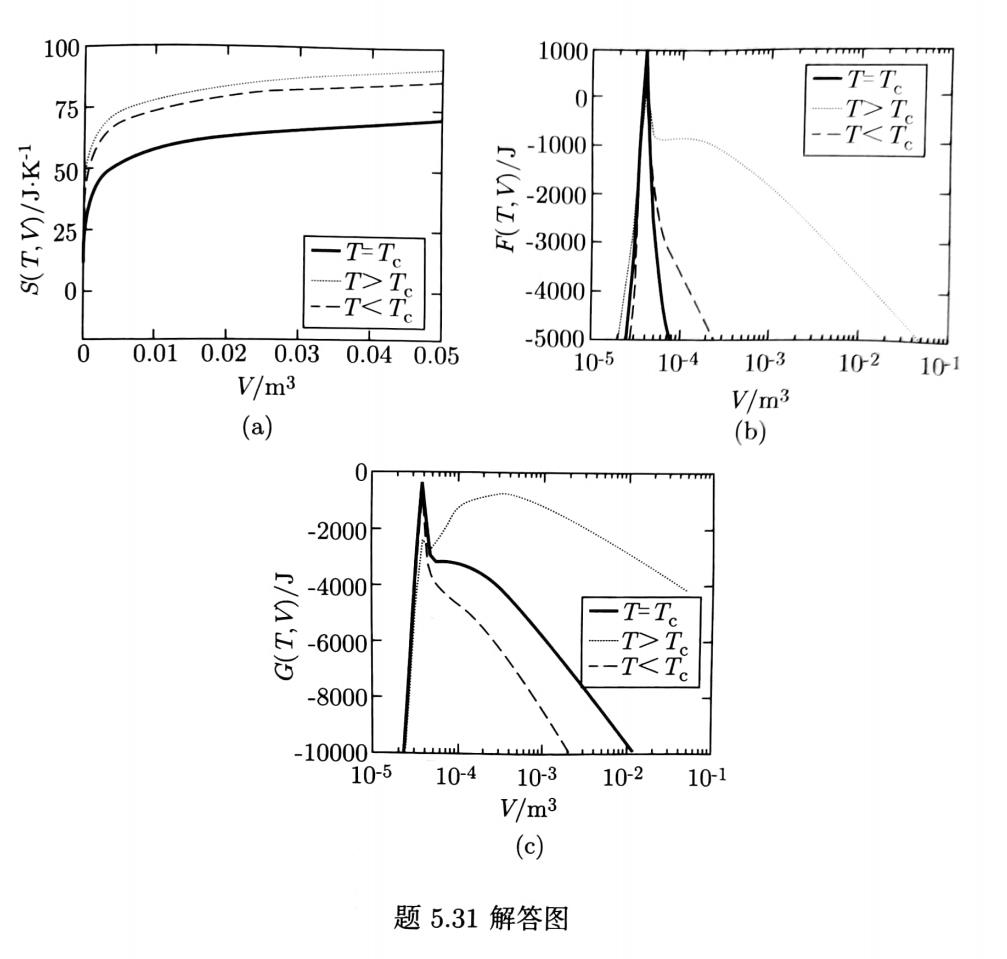
\includegraphics[width=0.6\textwidth]{image.png}
  \caption{题 5.31 解答图 (a)(b)(c)，范德瓦尔斯气体与理想气体的 S(V), F(V), G(V) 曲线比较}
  \label{fig:image}
\end{figure}



\subsubsection{题 5.32}

\textbf{题目}：试证明：范德瓦尔斯气体的定容热容量只是温度的函数，与系统的体积无关。

\textbf{证明}：由定义 $C_V=T\!\left(\dfrac{\partial S}{\partial T}\right)_V$ 和麦克斯韦关系 $\left(\dfrac{\partial S}{\partial V}\right)_T=\left(\dfrac{\partial p}{\partial T}\right)_V$，知
\[
\left(\frac{\partial C_V}{\partial V}\right)_T
=T\frac{\partial}{\partial V}\!\left(\frac{\partial S}{\partial T}\right)_V
=T\left[\frac{\partial}{\partial T}\!\left(\frac{\partial S}{\partial V}\right)_T\right]_V
=T\left[\frac{\partial}{\partial T}\!\left(\frac{\partial p}{\partial T}\right)_V\right]_V
=T\left(\frac{\partial^2 p}{\partial T^2}\right)_V
\]

对于范德瓦尔斯气体，由其状态方程
\[
\left(p+\frac{\nu^2 a}{V^2}\right)(V-\nu b)=\nu RT
\]
知
\[
p=\frac{\nu RT}{V-\nu b}-\frac{\nu^2 a}{V^2}
\]

于是有
\[
\left(\frac{\partial p}{\partial T}\right)_V=\frac{\nu R}{V-\nu b},\qquad
\left(\frac{\partial^2 p}{\partial T^2}\right)_V=0
\]

因此
\[
\left(\frac{\partial C_V}{\partial V}\right)_T=0
\]

这表明，\textbf{范德瓦尔斯气体的定体热容只是温度的函数，与系统的体积无关}。
\[
\boxed{\left(\frac{\partial C_V}{\partial V}\right)_T=0}
\]


\subsection{热力学势}

\subsubsection{基本概念}

\paragraph{热力学势}
可将态函数 $p,V,T,S$ 进行组合以构造其他态函数，这些由状态参量组合而成的函数具有能量量纲，称为\textbf{热力学势}。

大多数组合没有多大用处，常用的三种热力学势为：

\begin{center}
\begin{tabular}{c|c|c}
\hline
名称 & 定义式 & 自然变量 \\
\hline
焓 & $H=U+pV$ & $S,p$ \\
亥姆霍兹自由能 & $F=U-TS$ & $T,V$ \\
吉布斯自由焓 & $G=H-TS$ & $T,p$ \\
\hline
\end{tabular}
\end{center}

\subsubsection{焓}

由热力学基本方程 $\mathrm{d}U=T\,\mathrm{d}S-p\,\mathrm{d}V$，对焓 $H=U+pV$ 求全微分：
\[
\mathrm{d}H=\mathrm{d}U+p\,\mathrm{d}V+V\,\mathrm{d}p
=T\,\mathrm{d}S-p\,\mathrm{d}V+p\,\mathrm{d}V+V\,\mathrm{d}p
=T\,\mathrm{d}S+V\,\mathrm{d}p
\]

因此焓可视为以 $S,p$ 为自然变量的态函数：$H=H(S,p)$。

\paragraph{等压过程}
在等压过程中 $\mathrm{d}p=0$，于是 $\mathrm{d}H=T\,\mathrm{d}S$。
对可逆等压过程，$\mathrm{d}H=\mathrm{d}Q_{\mathrm{rev}}=C_p\,\mathrm{d}T$，积分得
\[
\Delta H=\int_{T_1}^{T_2}C_p\,\mathrm{d}T
\]

\paragraph{一阶偏导数}
由 $\mathrm{d}H=T\,\mathrm{d}S+V\,\mathrm{d}p$ 直接读出：
\[
T=\left(\frac{\partial H}{\partial S}\right)_p,\qquad
V=\left(\frac{\partial H}{\partial p}\right)_S
\]

\paragraph{缺陷}
$U$ 和 $H$ 的自然变量中均包含熵 $S$，而 $S$ 在实验室中不易直接测量和控制。

\subsubsection{亥姆霍兹自由能}

由 $F=U-TS$，求全微分并利用 $\mathrm{d}U=T\,\mathrm{d}S-p\,\mathrm{d}V$：
\[
\mathrm{d}F=\mathrm{d}U-T\,\mathrm{d}S-S\,\mathrm{d}T
=T\,\mathrm{d}S-p\,\mathrm{d}V-T\,\mathrm{d}S-S\,\mathrm{d}T
=-S\,\mathrm{d}T-p\,\mathrm{d}V
\]

因此自由能可视为以 $T,V$ 为自然变量的态函数：$F=F(T,V)$。

\paragraph{等温过程}
在等温过程中 $\mathrm{d}T=0$，于是 $\mathrm{d}F=-p\,\mathrm{d}V$，积分得
\[
\Delta F=-\int_{V_1}^{V_2}p\,\mathrm{d}V
\]

\paragraph{物理意义}
\begin{itemize}[leftmargin=2em]
  \item $\Delta F>0$：环境对系统做了可逆功；
  \item $\Delta F<0$：系统对环境做了可逆功。
\end{itemize}

\paragraph{一阶偏导数}
\[
S=-\left(\frac{\partial F}{\partial T}\right)_V,\qquad
p=-\left(\frac{\partial F}{\partial V}\right)_T
\]

\paragraph{等温等体过程}
在等温等体条件下，$\mathrm{d}T=0,\,\mathrm{d}V=0$，故
\[
\boxed{\mathrm{d}F=0}
\]
即自由能在等温等体过程中守恒。

\subsubsection{吉布斯函数（自由焓）}

由 $G=H-TS$，求全微分并利用 $\mathrm{d}H=T\,\mathrm{d}S+V\,\mathrm{d}p$：
\[
\mathrm{d}G=\mathrm{d}H-T\,\mathrm{d}S-S\,\mathrm{d}T
=T\,\mathrm{d}S+V\,\mathrm{d}p-T\,\mathrm{d}S-S\,\mathrm{d}T
=-S\,\mathrm{d}T+V\,\mathrm{d}p
\]

因此吉布斯函数可视为以 $T,p$ 为自然变量的态函数：$G=G(T,p)$。

\paragraph{特点}
在大多数实验中，温度 $T$ 和压强 $p$ 是最容易操作和控制的参量，因此 $G(T,p)$ 在实际应用中极为方便。

\paragraph{等温等压过程}
在等温等压条件下，$\mathrm{d}T=0,\,\mathrm{d}p=0$，故
\[
\boxed{\mathrm{d}G=0}
\]
即吉布斯函数在等温等压过程中守恒。

\paragraph{一阶偏导数}
\[
S=-\left(\frac{\partial G}{\partial T}\right)_p,\qquad
V=\left(\frac{\partial G}{\partial p}\right)_T
\]


% ============================================================
\subsection{热力学基本方程与一阶偏导}
% ============================================================

\subsubsection{四个基本方程}

综合以上讨论，得到封闭系统（只考虑体积功）的四个\textbf{热力学基本方程}：

\begin{align}
\mathrm{d}U &= T\,\mathrm{d}S-p\,\mathrm{d}V \tag{1}\\[4pt]
\mathrm{d}H &= T\,\mathrm{d}S+V\,\mathrm{d}p \tag{2}\\[4pt]
\mathrm{d}F &= -S\,\mathrm{d}T-p\,\mathrm{d}V \tag{3}\\[4pt]
\mathrm{d}G &= -S\,\mathrm{d}T+V\,\mathrm{d}p \tag{4}
\end{align}

\subsubsection{一阶偏导数关系}

由上述全微分表达式，直接读出各热力学势对其自然变量的一阶偏导数：

\begin{center}
\begin{tabular}{c|c|c}
\hline
热力学势 & 对第一自然变量的偏导 & 对第二自然变量的偏导 \\
\hline
$U(S,V)$ & $\displaystyle\left(\frac{\partial U}{\partial S}\right)_V=T$ & $\displaystyle\left(\frac{\partial U}{\partial V}\right)_S=-p$ \\[8pt]
$H(S,p)$ & $\displaystyle\left(\frac{\partial H}{\partial S}\right)_p=T$ & $\displaystyle\left(\frac{\partial H}{\partial p}\right)_S=V$ \\[8pt]
$F(T,V)$ & $\displaystyle\left(\frac{\partial F}{\partial T}\right)_V=-S$ & $\displaystyle\left(\frac{\partial F}{\partial V}\right)_T=-p$ \\[8pt]
$G(T,p)$ & $\displaystyle\left(\frac{\partial G}{\partial T}\right)_p=-S$ & $\displaystyle\left(\frac{\partial G}{\partial p}\right)_T=V$ \\
\hline
\end{tabular}
\end{center}


% ============================================================
\subsection{吉布斯--亥姆霍兹方程}
% ============================================================

利用一阶偏导数关系，可将内能 $U$ 和焓 $H$ 表示为自由能和吉布斯函数对温度的导数形式。

\paragraph{由内能 $U=F+TS$}
因为 $S=-\left(\dfrac{\partial F}{\partial T}\right)_V$，代入得
\[
U=F-T\left(\frac{\partial F}{\partial T}\right)_V
=-T^2\left(\frac{\partial(F/T)}{\partial T}\right)_V
\]

\paragraph{由焓 $H=G+TS$}
因为 $S=-\left(\dfrac{\partial G}{\partial T}\right)_p$，代入得
\[
H=G-T\left(\frac{\partial G}{\partial T}\right)_p
=-T^2\left(\frac{\partial(G/T)}{\partial T}\right)_p
\]

\paragraph{总结}
\[
\boxed{U=-T^2\left(\frac{\partial(F/T)}{\partial T}\right)_V},\qquad
\boxed{H=-T^2\left(\frac{\partial(G/T)}{\partial T}\right)_p}
\]

这两个关系在化学热力学中非常有用，常用于由自由能数据计算反应热。

% ============================================================
\subsection{熵关于温度的偏导数与热容}
% ============================================================

利用链式法则与一阶偏导数关系，可建立定容/定压热容与熵对温度偏导数之间的联系。

\paragraph{定容热容}
\[
C_V=\left(\frac{\partial U}{\partial T}\right)_V
=\left(\frac{\partial U}{\partial S}\right)_V\left(\frac{\partial S}{\partial T}\right)_V
=T\left(\frac{\partial S}{\partial T}\right)_V
\quad\Longrightarrow\quad
\boxed{\left(\frac{\partial S}{\partial T}\right)_V=\frac{C_V}{T}}
\]

\paragraph{定压热容}
\[
C_p=\left(\frac{\partial H}{\partial T}\right)_p
=\left(\frac{\partial H}{\partial S}\right)_p\left(\frac{\partial S}{\partial T}\right)_p
=T\left(\frac{\partial S}{\partial T}\right)_p
\quad\Longrightarrow\quad
\boxed{\left(\frac{\partial S}{\partial T}\right)_p=\frac{C_p}{T}}
\]


% ============================================================
\subsection{麦克斯韦关系（Maxwell Relations）}
% ============================================================

\subsubsection{推导依据}

对于解析函数（态函数），混合偏导数与求导顺序无关。将四个热力学基本方程分别应用于这一性质，即可得到麦克斯韦关系。

\subsubsection{四个麦克斯韦关系}

\begin{enumerate}[leftmargin=2em]
  \item \textbf{由 $\mathrm{d}U=T\,\mathrm{d}S-p\,\mathrm{d}V$}\\
  视 $U=U(S,V)$，则 $\dfrac{\partial^2 U}{\partial V\partial S}=\dfrac{\partial^2 U}{\partial S\partial V}$，即
  \[
  \boxed{\left(\frac{\partial T}{\partial V}\right)_S=-\left(\frac{\partial p}{\partial S}\right)_V}
  \]

  \item \textbf{由 $\mathrm{d}H=T\,\mathrm{d}S+V\,\mathrm{d}p$}\\
  视 $H=H(S,p)$，则
  \[
  \boxed{\left(\frac{\partial T}{\partial p}\right)_S=\left(\frac{\partial V}{\partial S}\right)_p}
  \]

  \item \textbf{由 $\mathrm{d}F=-S\,\mathrm{d}T-p\,\mathrm{d}V$}\\
  视 $F=F(T,V)$，则
  \[
  \boxed{\left(\frac{\partial S}{\partial V}\right)_T=\left(\frac{\partial p}{\partial T}\right)_V}
  \]

  \item \textbf{由 $\mathrm{d}G=-S\,\mathrm{d}T+V\,\mathrm{d}p$}\\
  视 $G=G(T,p)$，则
  \[
  \boxed{\left(\frac{\partial S}{\partial p}\right)_T=-\left(\frac{\partial V}{\partial T}\right)_p}
  \]
\end{enumerate}


% ============================================================
\subsection{内能与状态方程之间的关系}
% ============================================================

\subsubsection{推导}

以 $T,V$ 为独立变量，熵的全微分为
\[
\mathrm{d}S=\left(\frac{\partial S}{\partial T}\right)_V\mathrm{d}T
+\left(\frac{\partial S}{\partial V}\right)_T\mathrm{d}V
=\frac{C_V}{T}\,\mathrm{d}T+\left(\frac{\partial p}{\partial T}\right)_V\mathrm{d}V
\]
其中第二步利用了 $\left(\dfrac{\partial S}{\partial T}\right)_V=\dfrac{C_V}{T}$ 及麦克斯韦关系 $\left(\dfrac{\partial S}{\partial V}\right)_T=\left(\dfrac{\partial p}{\partial T}\right)_V$。

另一方面，由热力学基本方程 $\mathrm{d}U=T\,\mathrm{d}S-p\,\mathrm{d}V$，将 $U=U(T,V)$ 展开：
\[
\mathrm{d}U=\left(\frac{\partial U}{\partial T}\right)_V\mathrm{d}T
+\left(\frac{\partial U}{\partial V}\right)_T\mathrm{d}V
\]
于是
\[
T\,\mathrm{d}S=\mathrm{d}U+p\,\mathrm{d}V
=\left(\frac{\partial U}{\partial T}\right)_V\mathrm{d}T
+\left[\left(\frac{\partial U}{\partial V}\right)_T+p\right]\mathrm{d}V
\]
两边除以 $T$ 得
\[
\mathrm{d}S=\frac{C_V}{T}\,\mathrm{d}T
+\frac{1}{T}\left[\left(\frac{\partial U}{\partial V}\right)_T+p\right]\mathrm{d}V
\]

\subsubsection{内能公式}

比较以上两种 $\mathrm{d}S$ 表达式中 $\mathrm{d}V$ 的系数，得
\[
\left(\frac{\partial p}{\partial T}\right)_V
=\frac{1}{T}\left[\left(\frac{\partial U}{\partial V}\right)_T+p\right]
\]

整理即得\textbf{内能公式}：
\[
\boxed{\left(\frac{\partial U}{\partial V}\right)_T
=T\left(\frac{\partial p}{\partial T}\right)_V-p}
\]

该公式将内能对体积的偏导数与状态方程联系起来。对理想气体 $p=\dfrac{\nu RT}{V}$，有 $\left(\dfrac{\partial p}{\partial T}\right)_V=\dfrac{\nu R}{V}$，代入得
\[
\left(\frac{\partial U}{\partial V}\right)_T
=T\frac{\nu R}{V}-p=0
\]
即理想气体内能只与温度有关，与体积无关。


% ============================================================
\subsection{焓与状态方程之间的关系}
% ============================================================

\subsubsection{推导}

以 $T,p$ 为独立变量，熵的全微分为
\[
\mathrm{d}S=\left(\frac{\partial S}{\partial T}\right)_p\mathrm{d}T
+\left(\frac{\partial S}{\partial p}\right)_T\mathrm{d}p
=\frac{C_p}{T}\,\mathrm{d}T-\left(\frac{\partial V}{\partial T}\right)_p\mathrm{d}p
\]
其中利用了 $\left(\dfrac{\partial S}{\partial p}\right)_T=-\left(\dfrac{\partial V}{\partial T}\right)_p$（麦克斯韦关系）。

另一方面，由 $\mathrm{d}H=T\,\mathrm{d}S+V\,\mathrm{d}p$，将 $H=H(T,p)$ 展开：
\[
\mathrm{d}H=\left(\frac{\partial H}{\partial T}\right)_p\mathrm{d}T
+\left(\frac{\partial H}{\partial p}\right)_T\mathrm{d}p
\]
于是
\[
T\,\mathrm{d}S=\mathrm{d}H-V\,\mathrm{d}p
=\left(\frac{\partial H}{\partial T}\right)_p\mathrm{d}T
+\left[\left(\frac{\partial H}{\partial p}\right)_T-V\right]\mathrm{d}p
\]
两边除以 $T$ 得
\[
\mathrm{d}S=\frac{C_p}{T}\,\mathrm{d}T
+\frac{1}{T}\left[\left(\frac{\partial H}{\partial p}\right)_T-V\right]\mathrm{d}p
\]

\subsubsection{焓公式}

比较以上两种 $\mathrm{d}S$ 表达式中 $\mathrm{d}p$ 的系数，得
\[
-\left(\frac{\partial V}{\partial T}\right)_p
=\frac{1}{T}\left[\left(\frac{\partial H}{\partial p}\right)_T-V\right]
\]

整理即得\textbf{焓公式}：
\[
\boxed{\left(\frac{\partial H}{\partial p}\right)_T
=-T\left(\frac{\partial V}{\partial T}\right)_p+V}
\]

该公式将焓对压强的偏导数与状态方程联系起来。对理想气体 $V=\dfrac{\nu RT}{p}$，有 $\left(\dfrac{\partial V}{\partial T}\right)_p=\dfrac{\nu R}{p}$，代入得
\[
\left(\frac{\partial H}{\partial p}\right)_T
=-T\frac{\nu R}{p}+V=0
\]
即理想气体焓只与温度有关，与压强无关。

% ============================================================
\subsection{范德瓦尔斯气体的内能和焓}
% ============================================================

\subsubsection{范德瓦尔斯气体的内能}

范德瓦尔斯气体的状态方程为
\[
\left(p+\frac{\nu^2 a}{V^2}\right)(V-\nu b)=\nu RT
\quad\Longrightarrow\quad
p=\frac{\nu RT}{V-\nu b}-\frac{\nu^2 a}{V^2}
\]

利用内能公式 $\displaystyle\left(\frac{\partial U}{\partial V}\right)_T=T\left(\frac{\partial p}{\partial T}\right)_V-p$：
\[
\left(\frac{\partial p}{\partial T}\right)_V=\frac{\nu R}{V-\nu b}
\]
\[
T\left(\frac{\partial p}{\partial T}\right)_V-p
=\frac{\nu RT}{V-\nu b}-\left(\frac{\nu RT}{V-\nu b}-\frac{\nu^2 a}{V^2}\right)
=\frac{\nu^2 a}{V^2}
\]

因此
\[
\left(\frac{\partial U}{\partial V}\right)_T=\frac{\nu^2 a}{V^2}
\]

积分得范德瓦尔斯气体的内能：
\[
\boxed{U(T,V)=\int C_V\,\mathrm{d}T-\frac{\nu^2 a}{V}+U_0}
\]

\subsubsection{范德瓦尔斯气体的焓}

由 $H=U+pV$：
\[
H(T,V)=\int C_V\,\mathrm{d}T-\frac{\nu^2 a}{V}+U_0+pV
\]

利用状态方程 $pV=\dfrac{\nu RTV}{V-\nu b}-\dfrac{\nu^2 a}{V}$，代入得
\[
\boxed{H(T,V)=\int C_V\,\mathrm{d}T+\frac{\nu RTV}{V-\nu b}-\frac{2\nu^2 a}{V}+H_0}
\]


% ============================================================
\subsection{化学势与相平衡}
% ============================================================

\subsubsection{化学势的定义}

对于封闭系统（$N=\text{const}$），吉布斯函数的全微分为
\[
\mathrm{d}G=-S\,\mathrm{d}T+V\,\mathrm{d}p
\]

但实际上，$G$ 是广延量，当系统的粒子数目 $N$ 变化时，$G$ 还应依赖于 $\mathrm{d}N$。对开放系统，$G=G(T,p,N)$，应有
\[
\boxed{\mathrm{d}G=-S\,\mathrm{d}T+V\,\mathrm{d}p+\mu\,\mathrm{d}N}
\]

其中
\[
\boxed{\mu=\left(\frac{\partial G}{\partial N}\right)_{T,p}}
\]
称为\textbf{化学势}。

对于单相物质，每一个分子所占有的自由焓应该相等，即
\[
\mu=\left(\frac{\partial G}{\partial N}\right)_{T,p}=\text{const}
\quad\Longrightarrow\quad
\boxed{\mu=\frac{G}{N}}
\]

\subsubsection{相平衡条件}

在等温、等压条件下的平衡条件为 $\mathrm{d}G=0$。对于两相系统（1, 2），有
\[
(\mathrm{d}G)_{T,p}=\mu_1\,\mathrm{d}N_1+\mu_2\,\mathrm{d}N_2=0
\]

相变中保持质量守恒：$N=N_1+N_2$，故 $\mathrm{d}N_1+\mathrm{d}N_2=0$。代入得
\[
\mu_1\,\mathrm{d}N_1=-\mu_2\,\mathrm{d}N_2=\mu_2\,\mathrm{d}N_1
\]

因此
\[
\boxed{\mu_1=\mu_2}
\]

\textbf{结论}：在相平衡中，各相物质的化学势相等。


% ============================================================
\subsection{热力学第三定律}
% ============================================================

\subsubsection{绝对熵}

由玻尔兹曼熵公式
\[
S=k_B\ln\Omega
\]

热力学第三定律表述为：\textbf{任何纯物质在绝对零度时的熵值为零}，即
\[
\boxed{\lim_{T\to 0}S(T)=0}
\]

\subsubsection{绝对零度不可达到}

把水在三相点的温度降低 $273.16\ \mathrm{K}$ 就达到熵值为零的温度，因而把此状态的温度定为零（绝对温标）。

由于制冷系数 $\varepsilon=\dfrac{T_1}{T_2-T_1}$，当 $T_2\to 0$ 时 $\varepsilon\to 0$。因此，\textbf{不可能通过有限过程把一个物体的温度冷却到绝对零度}。这是热力学第三定律的另一个表述形式。

\newpage
% ============================================================
\section{第六章：液体}
% ============================================================

\subsection{液体的性质与分类}

\subsubsection{液体的定义}

液体：具有一定体积、没有弹性（没有切变模量）、没有一定形状、不易被压缩的可流动物体。

\subsubsection{液体的分类}

按分子间不同的作用力，液体可分为：

\begin{itemize}[leftmargin=2em]
  \item \textbf{范德瓦尔斯液体}：分子不具有电偶极矩。例：液态惰性气体（氦除外）、液态氢。
  \item \textbf{极性液体}：分子具有较大的电偶极矩。例：氯化氢液体、溴化氢液体。
  \item \textbf{缔合性液体}：分子间有很强的吸引作用，结构较稳固，黏滞性大。例：水、甘油。
  \item \textbf{金属液体}：存在自由电子，传热、导电性能较好。例：金属熔解形成的液体。
  \item \textbf{量子液体}：黏滞性消失，呈超流态等量子现象。例：液氦（$^4\mathrm{He}$）II。
  \item \textbf{液晶}：介于固态与液态之间的过渡状态（在一定温度区间内）。力学性质——具有流动性；光学性质——各向异性。
\end{itemize}

\subsection{液体的微观结构及研究方法}

\subsubsection{液体分子的排列方式}

液体分子的排列方式：\textbf{短程有序、长程无序}。

% [插图：液体（短程有序）与固体（晶体，长程有序）分子排列对比示意图]
\begin{figure}[htbp]
  \centering
  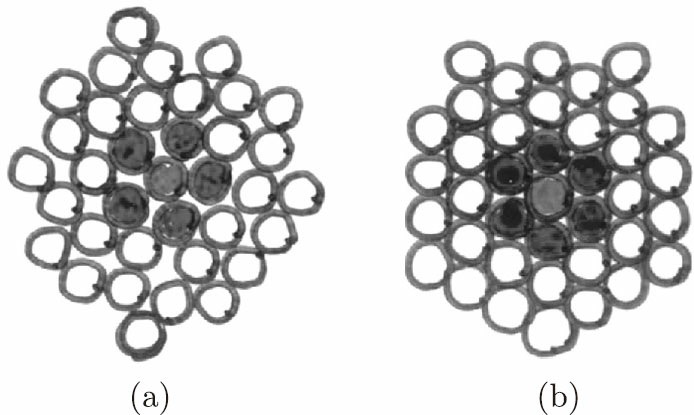
\includegraphics[width=0.6\textwidth]{liquid_structure.png}
  \caption{液体（短程有序）与固体（晶体，长程有序）分子排列对比示意图}
  \label{fig:liquid_structure}
\end{figure}

\subsubsection{排列方式的描述与实验观测}

利用X射线衍射方法测量液体汞及晶体汞的径向分布函数 $\rho(r)/\rho_0$。

% [插图：液体汞及晶体汞的径向分布函数曲线]
\begin{figure}[htbp]
  \centering
  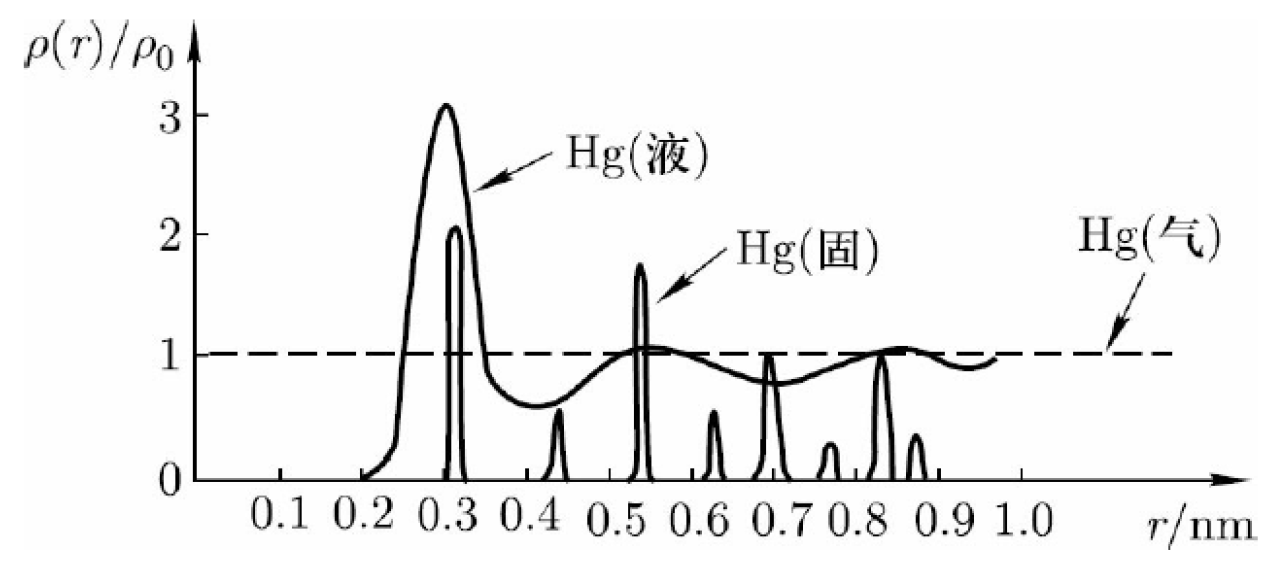
\includegraphics[width=0.45\textwidth]{radial_distribution_hg.png}
  \caption{利用X射线衍射方法测量的液体汞及晶体汞的径向分布函数}
  \label{fig:radial_distribution_hg}
\end{figure}

实验测得的液态氩的径向分布函数随温度变化：温度越高，有序性越差。

% [插图：液态氩在不同温度下的径向分布函数]
\begin{figure}[htbp]
  \centering
  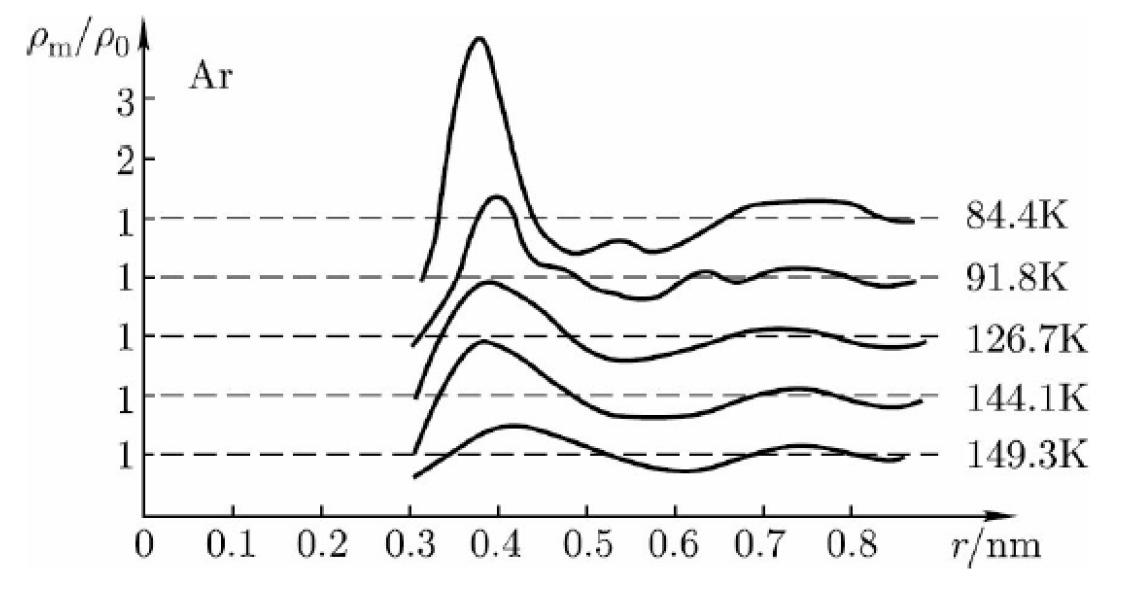
\includegraphics[width=0.45\textwidth]{radial_distribution_ar.png}
  \caption{实验测得的液态氩在不同温度下的径向分布函数}
  \label{fig:radial_distribution_ar}
\end{figure}

\subsection{液体分子的热运动}

\subsubsection{热运动模式}

液体分子的热运动模式：\textbf{仅在其平衡位置附近作振动}。

\subsubsection{热运动特点}

同一单元中液体分子的振动方向基本一致，不同单元中液体分子的振动方向各不相同。

\subsubsection{振动中心与时间}

振动中心及相应振动时间不定。液体分子在各个平衡位置振动时间的平均值为
\[
\boxed{\bar{\tau}=\bar{\tau}_0 e^{E_a/(k_BT)}}
\]
其中 $E_a$ 为激活能。

通常分子在一个单元平均振动 $10^2\sim 10^3$ 次。

\subsection{液体的热容量}

\subsubsection{实验规律}

实验表明：液体的定压热容量与固体的定压热容量相近
\[
C_p^{(L)}\approx C_p^{(S)}
\]

由杜隆--珀替定律：$C_{p,m}^{(L)}\approx 3R$。

\subsubsection{与温度的关系}

\begin{itemize}[leftmargin=2em]
  \item 一般随 $T$ 升高而增大，如乙醚等；
  \item 有些反而减少，如液态铅；
  \item 少数不单调，如：水在 $0^{\circ}\mathrm{C}\sim 75.98$，$35^{\circ}\mathrm{C}\sim 75.27$，$100^{\circ}\mathrm{C}\sim 75.95$（单位：$\mathrm{J/(mol\cdot K)}$）。
\end{itemize}

% [插图：某液体定压热容量随温度变化曲线，在312K附近出现极小值]
\begin{figure}[htbp]
  \centering
  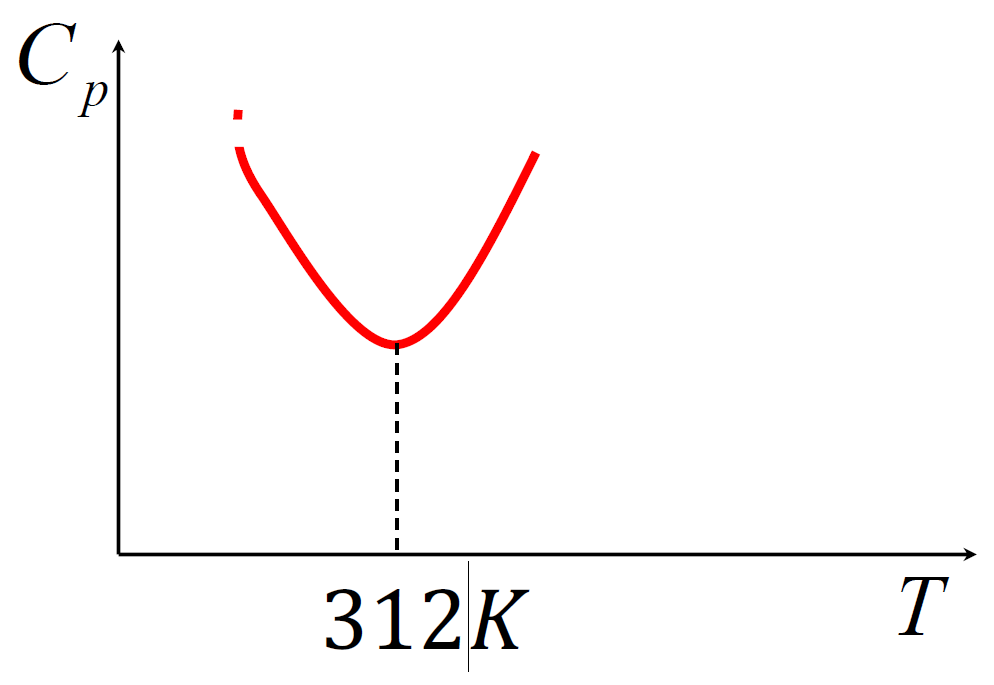
\includegraphics[width=0.4\textwidth]{liquid_heat_capacity.png}
  \caption{液体定压热容量随温度变化示意图（存在极小值）}
  \label{fig:liquid_heat_capacity}
\end{figure}

\subsubsection{定压与定容热容量的关系}

对固体 $C_V^{(S)}\approx C_p^{(S)}$；但对液体 $C_V^{(L)}\neq C_p^{(L)}$，且 $C_p^{(L)}-C_V^{(L)}\neq\text{常数}$。

对任意系统，由 $H=U+pV$ 得
\[
\left(\frac{\partial H}{\partial T}\right)_p=\left(\frac{\partial U}{\partial T}\right)_p+p\left(\frac{\partial V}{\partial T}\right)_p
\]

取 $U=U[T,V(T,p)]$，根据多元复合函数的偏导数法则：
\[
\left(\frac{\partial H}{\partial T}\right)_p=\left(\frac{\partial U}{\partial T}\right)_V+\left[p+\left(\frac{\partial U}{\partial V}\right)_T\right]\left(\frac{\partial V}{\partial T}\right)_p
\]

利用内能与状态方程之间的关系 $\displaystyle\left(\frac{\partial U}{\partial V}\right)_T=T\left(\frac{\partial p}{\partial T}\right)_V-p$，代入得
\[
\boxed{C_p-C_V=T\left(\frac{\partial p}{\partial T}\right)_V\left(\frac{\partial V}{\partial T}\right)_p}
\]

引入体膨胀系数 $\alpha=\dfrac{1}{V}\left(\dfrac{\partial V}{\partial T}\right)_p$、压强系数 $\beta=\dfrac{1}{p}\left(\dfrac{\partial p}{\partial T}\right)_V$ 及等温压缩系数 $\kappa_T=-\dfrac{1}{V}\left(\dfrac{\partial V}{\partial p}\right)_T$，上式可写成
\[
C_p-C_V=T(p\beta)(V\alpha)=VT\frac{\alpha^2}{\kappa_T}
\]

% ============================================================
\subsection{液体的表面性质}
% ============================================================

\subsubsection{表面与表面张力}

\paragraph{表面}
液体与自己的蒸汽或另一种介质接触的交界面称为\textbf{液体表面}。

表现现象：
\begin{itemize}[leftmargin=2em]
  \item 各种液滴呈球形；
  \item 水面上可以承受硬币、钢针等物体；
  \item 金属框内的细线在有无液面时呈不同的形状。
\end{itemize}

% [插图：表面张力演示示意图，包括液滴、硬币浮于水面、细线框实验]
\begin{figure}[htbp]
  \centering
  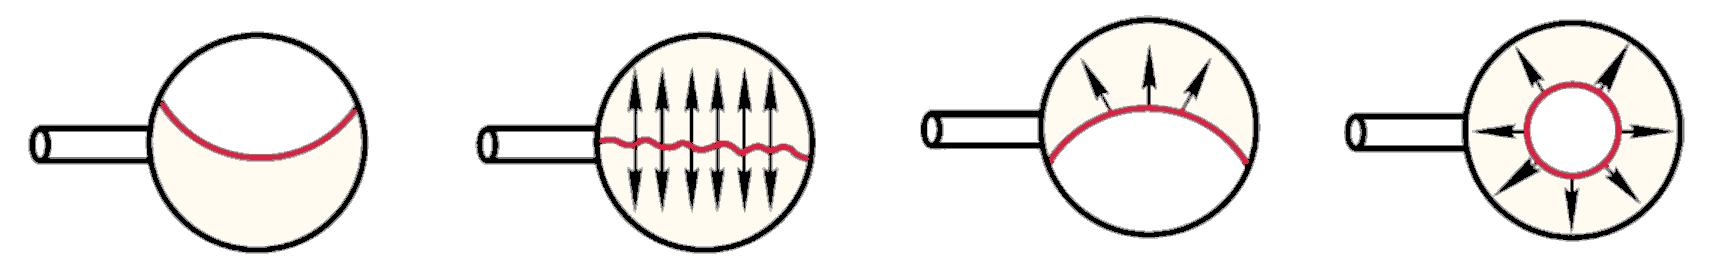
\includegraphics[width=0.5\textwidth]{surface_tension_demo.png}
  \caption{表面张力演示示意图}
  \label{fig:surface_tension_demo}
\end{figure}

\paragraph{表面张力}
在液体表面上想象画一条线，该线两侧的液面相互存在着拉力作用。这个位于液面内处处与此线垂直的拉力称为\textbf{表面张力}。

\begin{itemize}[leftmargin=2em]
  \item 与表面积的大小无关；
  \item 物理根源：表面层内分子之间的相互作用。
\end{itemize}

\subsubsection{表面张力系数——功}

外力作用，使表面积扩大的过程：

外力作功为
\[
\mathrm{d}W=f\,\mathrm{d}x=\alpha\cdot 2l\,\mathrm{d}x=\alpha\,\mathrm{d}A_s
\]
其中 $\mathrm{d}A_s=2l\,\mathrm{d}x$ 为液面增加的表面积（注意薄膜有两个表面）。

表面张力系数定义为
\[
\boxed{\alpha=\frac{\mathrm{d}W}{\mathrm{d}A_s}}
\]
即液面改变单位面积外界所作的功（等温、等体）。

表面张力（表面张力系数）与面积无关，仅与温度等条件有关。并且，\textbf{表面张力系数随温度升高而降低}：
\[
\frac{\mathrm{d}\alpha}{\mathrm{d}T}
=\frac{1-\eta}{N_A^{1/3}}\frac{\mathrm{d}\Lambda_m}{\mathrm{d}T}\left(\frac{\rho}{\mu}\right)^{2/3}<0
\]

\paragraph{物理解释}
\begin{itemize}[leftmargin=2em]
  \item 液体通常都具有热胀冷缩的性质，温度升高，分子间距通常会增大，摩尔汽化热减小；
  \item 从力的方面考虑：分子间距离增大，导致吸引力减小了，所以表面张力减小。
\end{itemize}

\subsubsection{题 6.2（李椿书 P241 第 2 题）}

\textbf{题目}：图是测表面张力系数的一种装置。先将薄铜片放入待测液体中，慢慢提起铜片，使它绝大部分都露出液面，刚要离开但还没有离开液面，测得此时所用的上提力 $F$，即可测得表面张力系数。设待测液体与铜片的接触角 $\theta=0$，铜片的质量 $m=5.0\times 10^{-4}\ \mathrm{kg}$，铜片的宽度 $l=3.977\times 10^{-2}\ \mathrm{m}$，厚度 $d=2.3\times 10^{-4}\ \mathrm{m}$，$F=1.07\times 10^{-2}\ \mathrm{N}$，求液体的表面张力系数。

% [插图：测表面张力系数装置示意图，铜片被提起时的受力分析]
\begin{figure}[htbp]
  \centering
  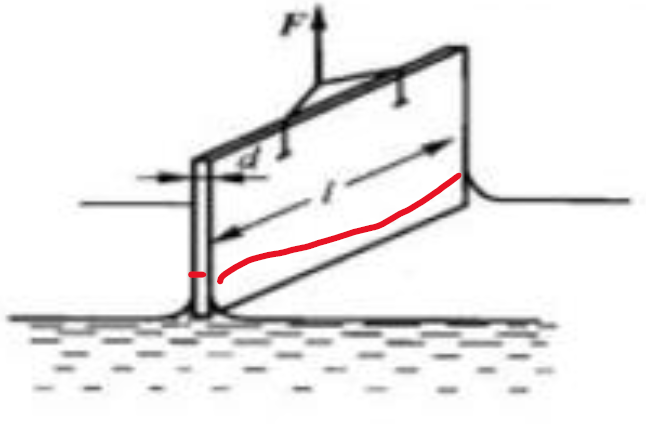
\includegraphics[width=0.35\textwidth]{surface_tension_measurement.png}
  \caption{题 6.2 测表面张力系数装置示意图}
  \label{fig:surface_tension_measurement}
\end{figure}

\textbf{解答}：

上提力等于铜片的重力与表面张力的和。铜片与液体的接触面为一个长为 $l$、宽为 $d$ 的矩形，因此表面张力为 $2\alpha(l+d)$（两侧均有液面）。

设液体的表面张力系数为 $\alpha$，有
\[
F=mg+2\alpha(l+d)
\]

故
\[
\alpha=\frac{F-mg}{2(l+d)}
=\frac{1.07\times 10^{-2}-5.0\times 10^{-4}\times 9.8}{2\times(3.977\times 10^{-2}+2.3\times 10^{-4})}
\approx 7.25\times 10^{-2}\ \mathrm{N\cdot m^{-1}}
\]

\[
\boxed{\alpha\approx 7.25\times 10^{-2}\ \mathrm{N/m}}
\]

\subsubsection{表面能（表面自由能）}

外力克服表面层中分子力的合力所作的功等于表面层中的分子引力势能的增加，这种增加的分子势能称为\textbf{表面自由能}，简称\textbf{表面能}。

等温过程 $\mathrm{d}W=\alpha\,\mathrm{d}A_s=\mathrm{d}(U-TS)=\mathrm{d}F$，得
\[
\boxed{\alpha=\left(\frac{\partial F_s}{\partial A_s}\right)_T}
\]

\paragraph{表面自由能和表面内能}

表面自由能 $F_s$ 为等温条件下外力在扩展表面时所作的功；但是 $F_s$ 不是表面内能。表明内能需要具体确定。

由 $U=F+TS$，$F_s=\alpha A_s$，得表面内能 $U_s=F_s+TS=\alpha A_s+TS$。

由 $\mathrm{d}F_s=\left(\dfrac{\partial F_s}{\partial A_s}\right)_T\mathrm{d}A_s+\left(\dfrac{\partial F_s}{\partial T}\right)_{A_s}\mathrm{d}T=\alpha\,\mathrm{d}A_s+A_s\left(\dfrac{\partial\alpha}{\partial T}\right)_{A_s}\mathrm{d}T$

及 $\mathrm{d}F_s=\mathrm{d}U_s-T\,\mathrm{d}S-S\,\mathrm{d}T$，结合第一定律 $\mathrm{d}U_s=\mathrm{d}Q+\mathrm{d}W=T\,\mathrm{d}S+\alpha\,\mathrm{d}A_s$，得 $\mathrm{d}F_s=\alpha\,\mathrm{d}A_s-S\,\mathrm{d}T$。

比较得
\[
S=-\left(\frac{\partial\alpha}{\partial T}\right)_{A_s}A_s
\]

表面内能
\[
U_s=\alpha A_s-TA_s\left(\frac{\partial\alpha}{\partial T}\right)_{A_s}
\]

表面内能密度
\[
\boxed{u_s=\alpha-T\left(\frac{\partial\alpha}{\partial T}\right)_{A_s}}
\]

\subsubsection{例题（类似题 6.4）}

\textbf{题目}：水和油的界面的表面张力系数为 $0.018\ \mathrm{N/m}$，为了使 $1.0\ \mathrm{g}$ 的油滴在水内散布成半径为 $10\ \mu\mathrm{m}$ 的小油滴，若散布过程是等温的，且油的密度为 $900\ \mathrm{kg/m^3}$，所需作的功为多少？

\textbf{解答}：

由表面张力的物理起因知，大油滴散布成大量小油滴时，与油滴相邻的水的表面自由能的增量等于外力所作的功，即有
\[
\Delta W=\Delta F=\alpha\Delta A_s
\]

其中 $\Delta A_s$ 是与油滴相邻的水的表面积的增量，即油滴表面积的增量。设大油滴的半径为 $R$，分裂成 $N$ 个小油滴，则
\[
\Delta A_s=4\pi(Nr^2-R^2)
\]

因油的质量不变，则有
\[
m=\frac{4}{3}\pi R^3\rho=N\cdot\frac{4}{3}\pi r^3\rho
\quad\Longrightarrow\quad
R^2=N^{2/3}r^2
\]

于是
\[
\Delta A_s=4\pi N^{2/3}r^2(N^{1/3}-1)\approx N\cdot 4\pi r^2
=\frac{m}{\frac{4}{3}\pi r^3\rho}\cdot 4\pi r^2
=\frac{3m}{r\rho}
\]

故
\[
\Delta W=\alpha\Delta A_s=\frac{3\alpha m}{r\rho}
=\frac{3\times 0.018\times(1.0\times 10^{-3})}{1\times 10^{-5}\times 900}
=6.0\times 10^{-3}\ \mathrm{J}
\]

\[
\boxed{\Delta W=6.0\times 10^{-3}\ \mathrm{J}}
\]

\subsubsection{弯曲液面内外压强差}

任意弯曲液面内外的压强差都可以表示为：
\[
\boxed{\Delta p=p_i-p_o=\alpha\left(\frac{1}{R_1}+\frac{1}{R_2}\right)}
\]
此即\textbf{拉普拉斯公式}（Laplace Formula）。

其中 $R_1,R_2$ 为过弯曲液面上一点的一对相互垂直正截口的曲率半径。

曲率中心在液体内 $R>0$，液体外 $R<0$。

正截口：包含曲面法线的平面与曲面的交线。

% [插图：弯曲液面上正截口与曲率半径示意图]
\begin{figure}[htbp]
  \centering
  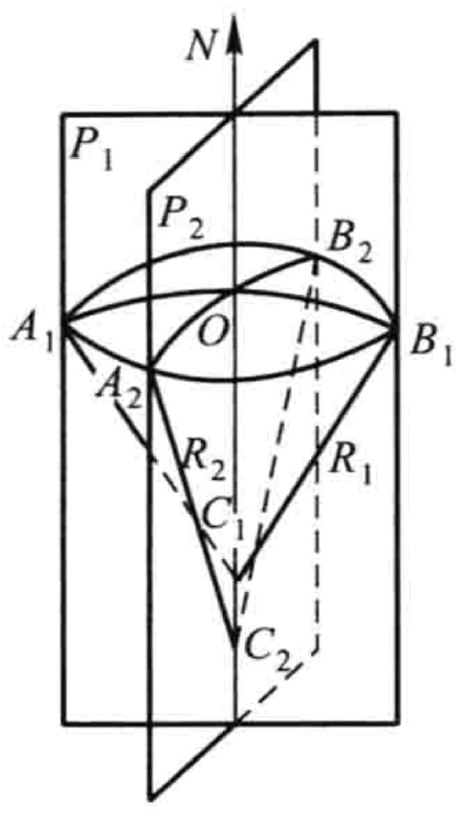
\includegraphics[width=0.4\textwidth]{laplace_pressure.png}
  \caption{弯曲液面正截口与曲率半径示意图}
  \label{fig:laplace}
\end{figure}

\paragraph{简单讨论}

\begin{itemize}[leftmargin=2em]
  \item \textbf{球形液面}：$R_1=R_2=R$，则
  \[
  p_i-p_o=\frac{2\alpha}{R}
  \]
  
  \item \textbf{柱形液面}：$R_1=R,\ R_2=\infty$，则
  \[
  p_i-p_o=\frac{\alpha}{R}
  \]
\end{itemize}

液面形状由其内部、外部及表面三部分的平衡所决定。

% [插图：球形液面、柱形液面压强差示意图，及液面凸凹形状示意]
\begin{figure}[htbp]
  \centering
  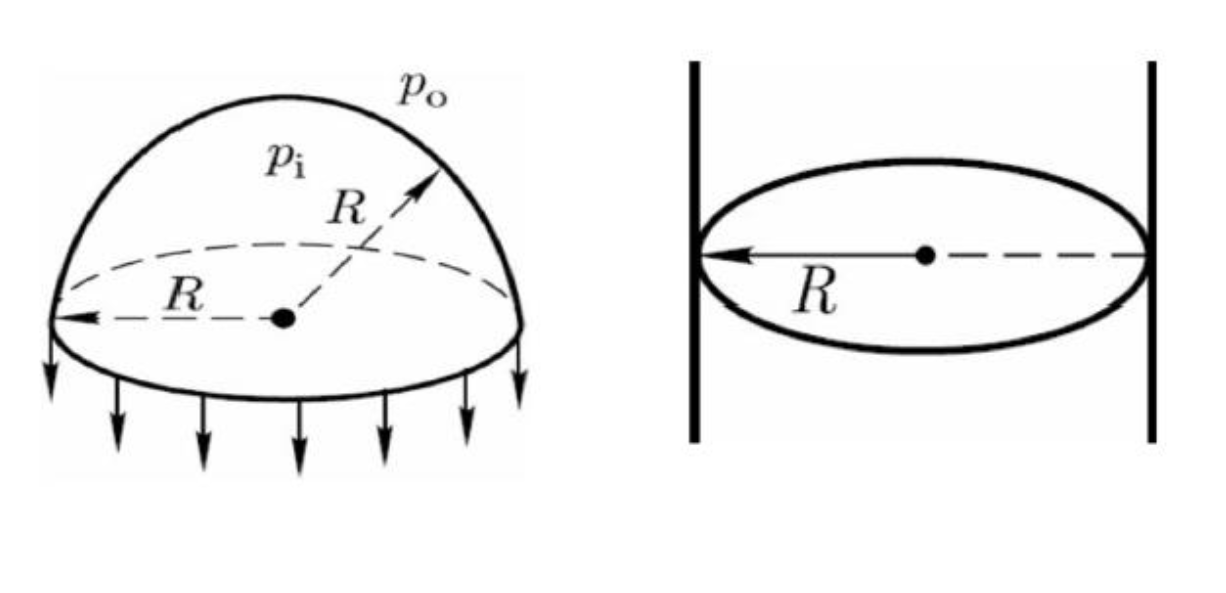
\includegraphics[width=0.5\textwidth]{laplace_discussion.png}
  \caption{球形液面与柱形液面压强差示意图}
  \label{fig:laplace_discussion}
\end{figure}

% ============================================================
\subsection{液面与固体接触处的表面现象}
% ============================================================

\subsubsection{润湿与不润湿现象}

\begin{itemize}[leftmargin=2em]
  \item \textbf{润湿}：液体与固体接触处，液体沿固体表面延展的现象，称为液体润湿固体。\textbf{接触角为锐角}。
  \item \textbf{不润湿}：液体与固体接触处，液体在固体表面上收缩的现象，称为液体不润湿固体。\textbf{接触角为钝角}。
\end{itemize}

能分清楚哪个是接触角？别弄反啦！

润湿、不润湿取决于相互接触的液体、固体的性质。

\begin{itemize}[leftmargin=2em]
  \item 水与玻璃是润湿的；
  \item 水银与玻璃是不润湿的。
\end{itemize}

生活中例子平时也要注意！

% ============================================================
\subsection{毛细现象}
% ============================================================

\subsubsection{毛细现象的定义}

毛细现象：将毛细管插入液体中，管内液面上升或下降的现象。

\paragraph{物理根源}
液体的\textbf{内聚力}与\textbf{附着力}的竞争引起，也就是由弯曲液面内外的压强差决定。

\begin{itemize}[leftmargin=2em]
  \item 附着力大于内聚力：液体\textbf{润湿}固体，液面上\textbf{凹}；液面``外''压强大于液面``内''压强，毛细管内液面\textbf{上升}。
  \item 内聚力大于附着力：液体\textbf{不润湿}固体，液面上\textbf{凸}；液面``内''压强大于液面``外''压强，毛细管内液面\textbf{下降}。
\end{itemize}

% [插图：毛细现象示意图，水在毛细管中上升、汞在毛细管中下降]
\begin{figure}[htbp]
\centering
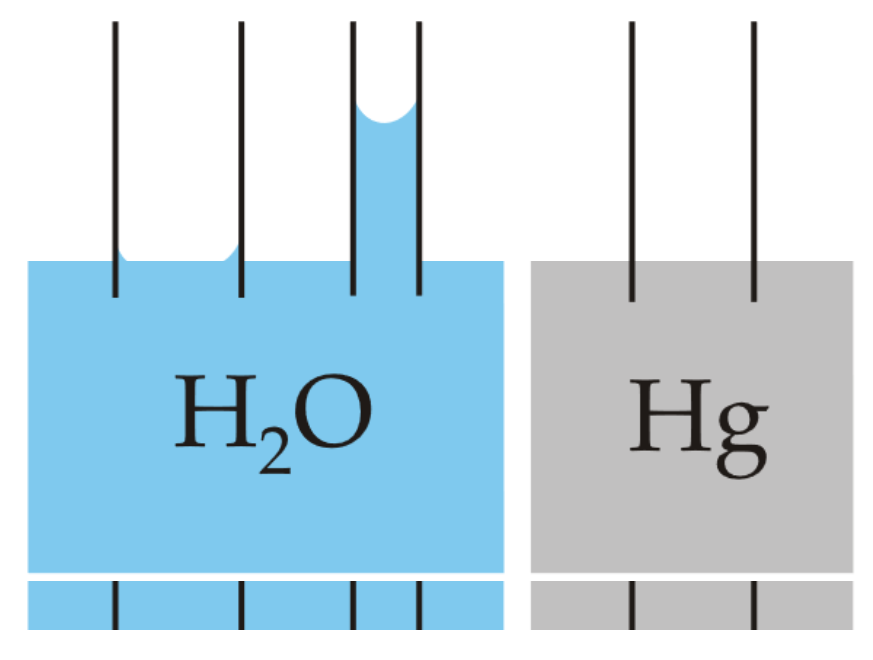
\includegraphics[width=0.4\textwidth]{capillary_tube.png}
\caption{竖直毛细管中的润湿（水）与不润湿（汞）}
\label{fig:capillary}
\end{figure}

\subsubsection{液面高度}

柱形毛细管中液面高度如图，设 A、D 分别是毛细管中液面内外紧靠液面的两点，则由弯曲液面内外的压强差知：
\[
p_A-p_D=\frac{2\alpha}{-R};\quad
p_A=p_D+\frac{2\alpha}{-R}=p_0-\frac{2\alpha}{R}
\]

C、O 分别为平液面部分液面附近内外两点，$p_C=p_O=p_0$。显然，$p_A<p_C$，所以液体会进入毛细管，引起其中液面上升。

设 B 为达到平衡时，管内液面下方与 C 同高处的一点，液面上升高度为 $h$，则
\[
p_B=p_A+\rho gh=p_0-\frac{2\alpha}{R}+\rho gh
\]

因为 $p_B=p_C=p_0$，于是有
\[
p_0-\frac{2\alpha}{R}+\rho gh=p_0
\]

即
\[
\boxed{h=\frac{2\alpha}{\rho gR}=\frac{2\alpha\cos\theta}{\rho gr}}
\]
其中 $r$ 为毛细管半径，$\theta$ 为接触角，$R=r/\cos\theta$。

\begin{itemize}[leftmargin=2em]
  \item $0\le\theta<\pi/2\ \Rightarrow\ h>0$，内部液面上升；
  \item $\pi/2<\theta\le\pi\ \Rightarrow\ h<0$，内部液面下降。
\end{itemize}

% [插图：毛细管液面高度推导示意图]
\begin{figure}[htbp]
  \centering
  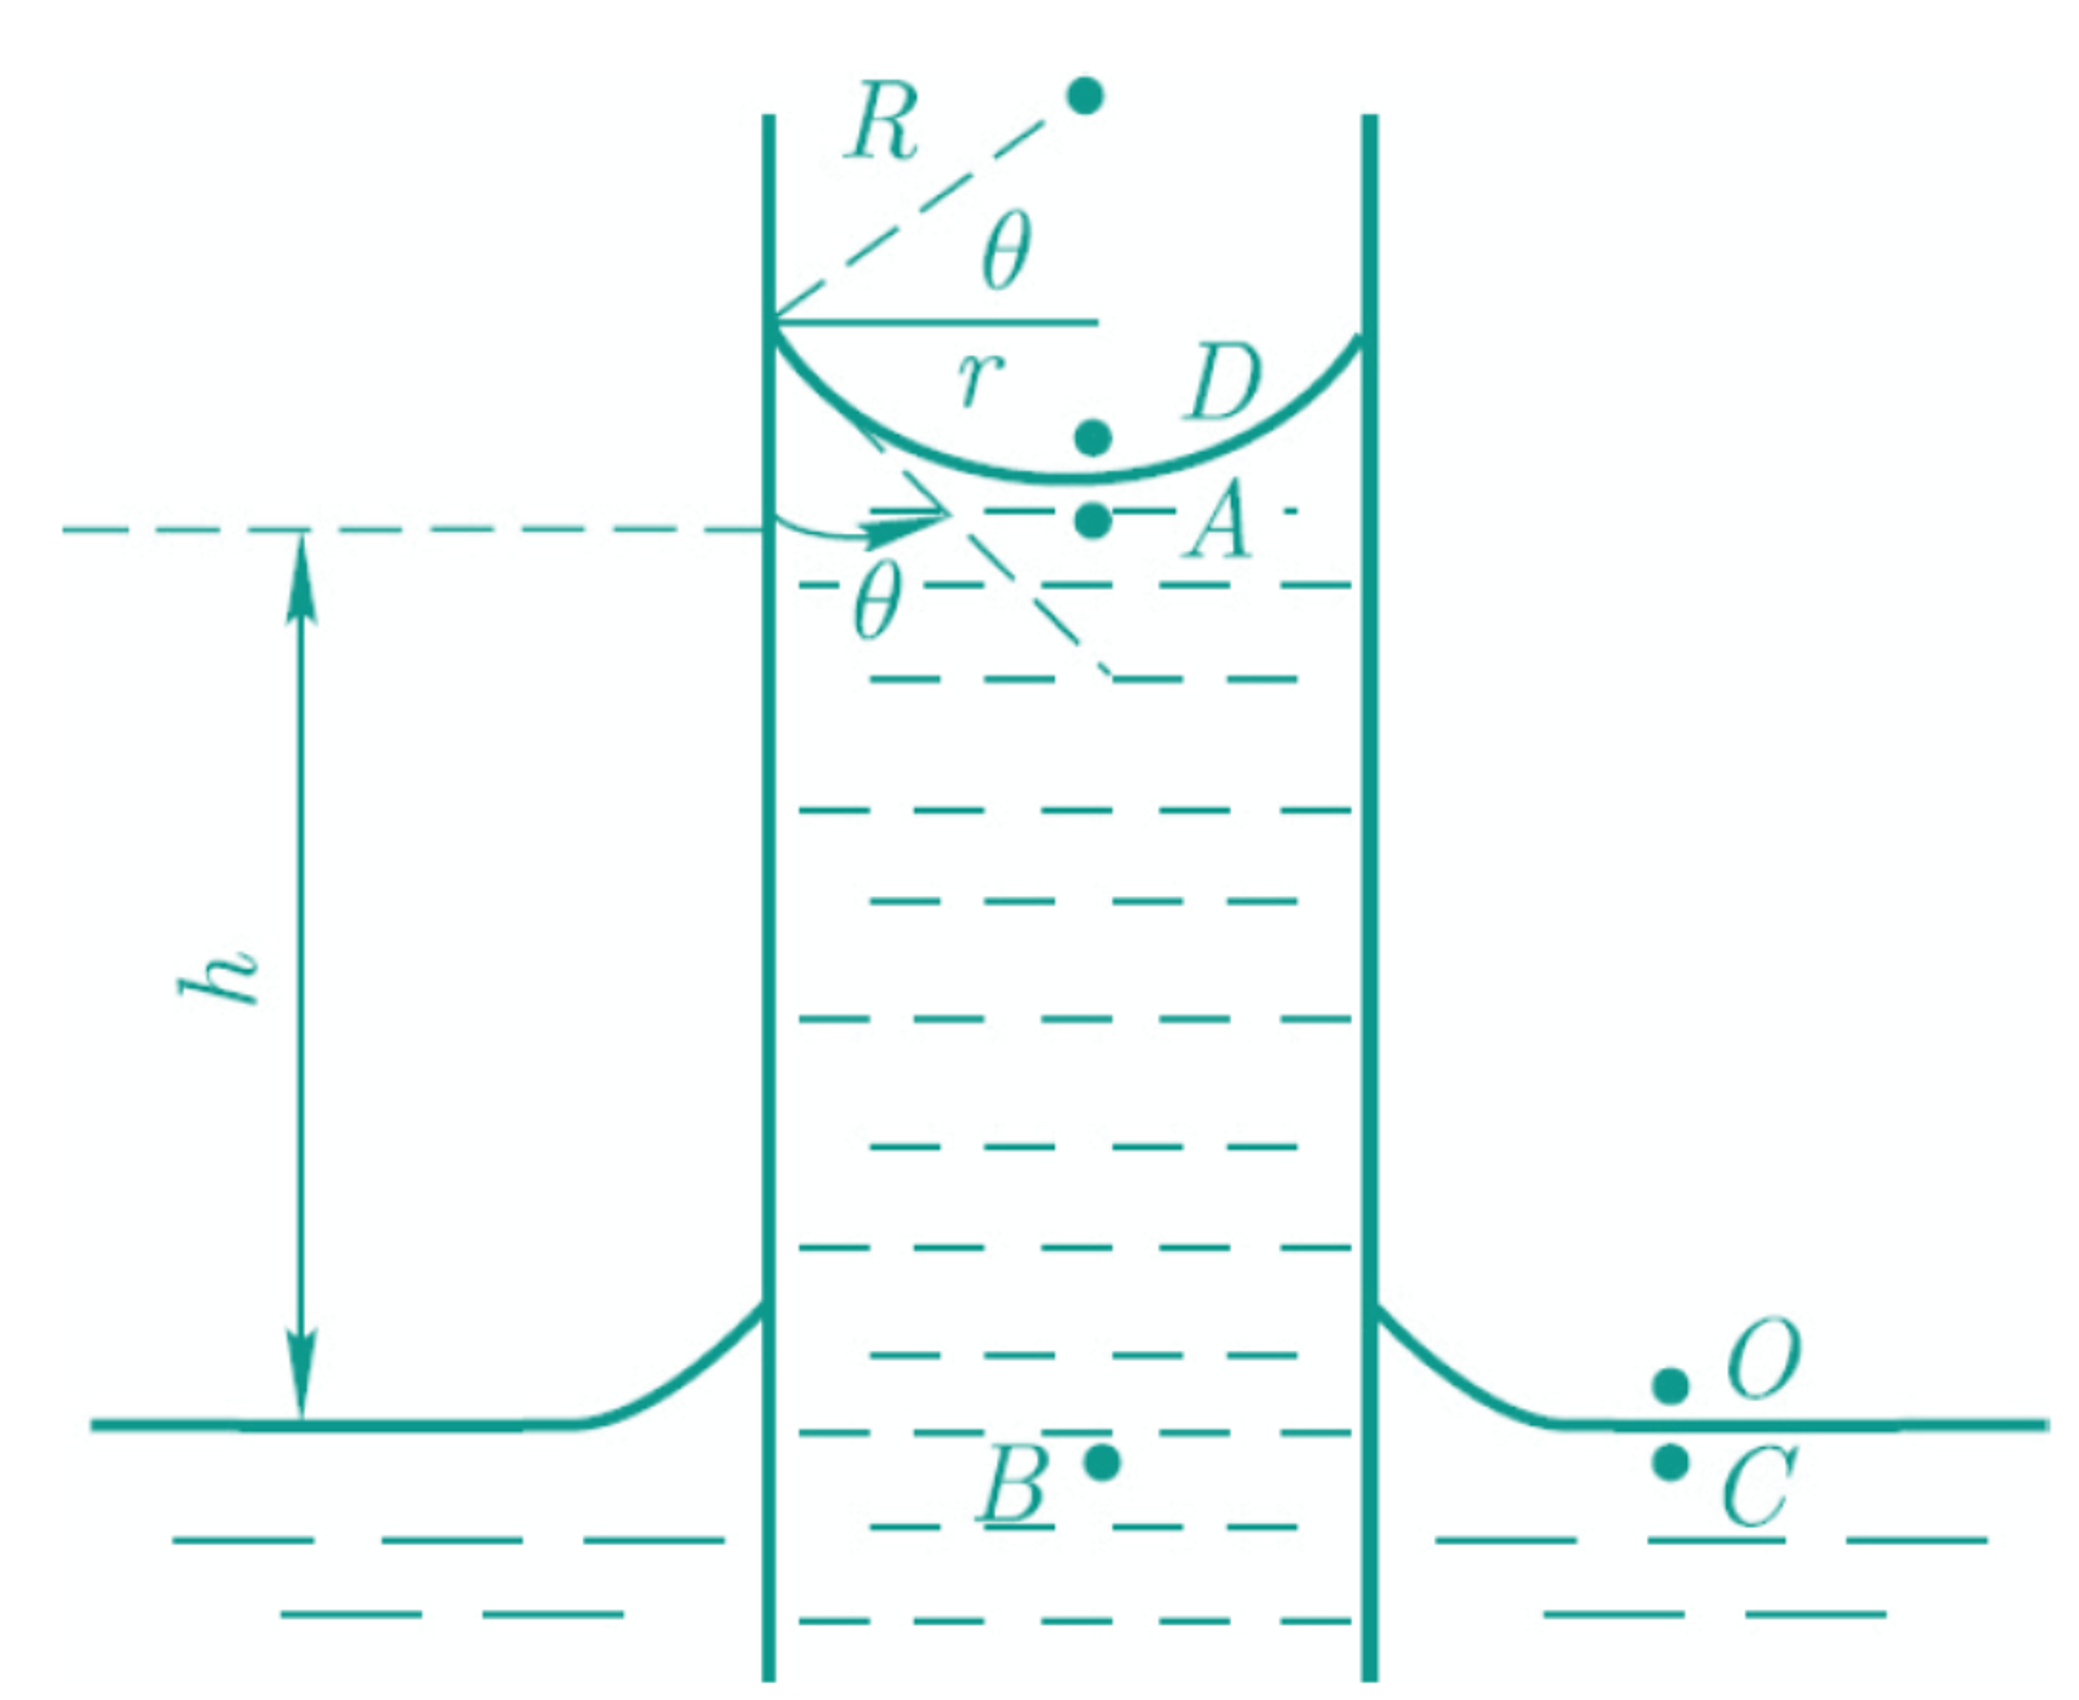
\includegraphics[width=0.4\textwidth]{capillary_height.png}
  \caption{毛细管液面高度推导示意图}
  \label{fig:capillary_height}
\end{figure}

\subsubsection{两平板间液面的高度}

\begin{itemize}[leftmargin=2em]
  \item 两平行板之间液面呈柱面，设两板之间间距为 $d$，则
  \[
  h=\frac{\alpha\cos\theta}{\rho g\dfrac{d}{2}}
  \quad\Rightarrow\quad
  \begin{cases}
  0\le\theta<\pi/2\ \Rightarrow\ h>0,\ \text{内部液面上升}\\[4pt]
  \pi/2<\theta\le\pi\ \Rightarrow\ h<0,\ \text{内部液面下降}
  \end{cases}
  \]
  
  \item 相交成很小夹角 $\varphi$ 的两平板间液面
  
  建立图示的坐标系，因为 $\varphi$ 很小，则 $x$ 处两板间距为 $d=x\varphi$。
  \[
  h=\frac{\alpha\cos\theta}{\rho g\dfrac{x\varphi}{2}}
  \]
  液面呈双曲面形。
\end{itemize}

% [插图：两平板间液面高度示意图]
\begin{figure}[htbp]
\centering
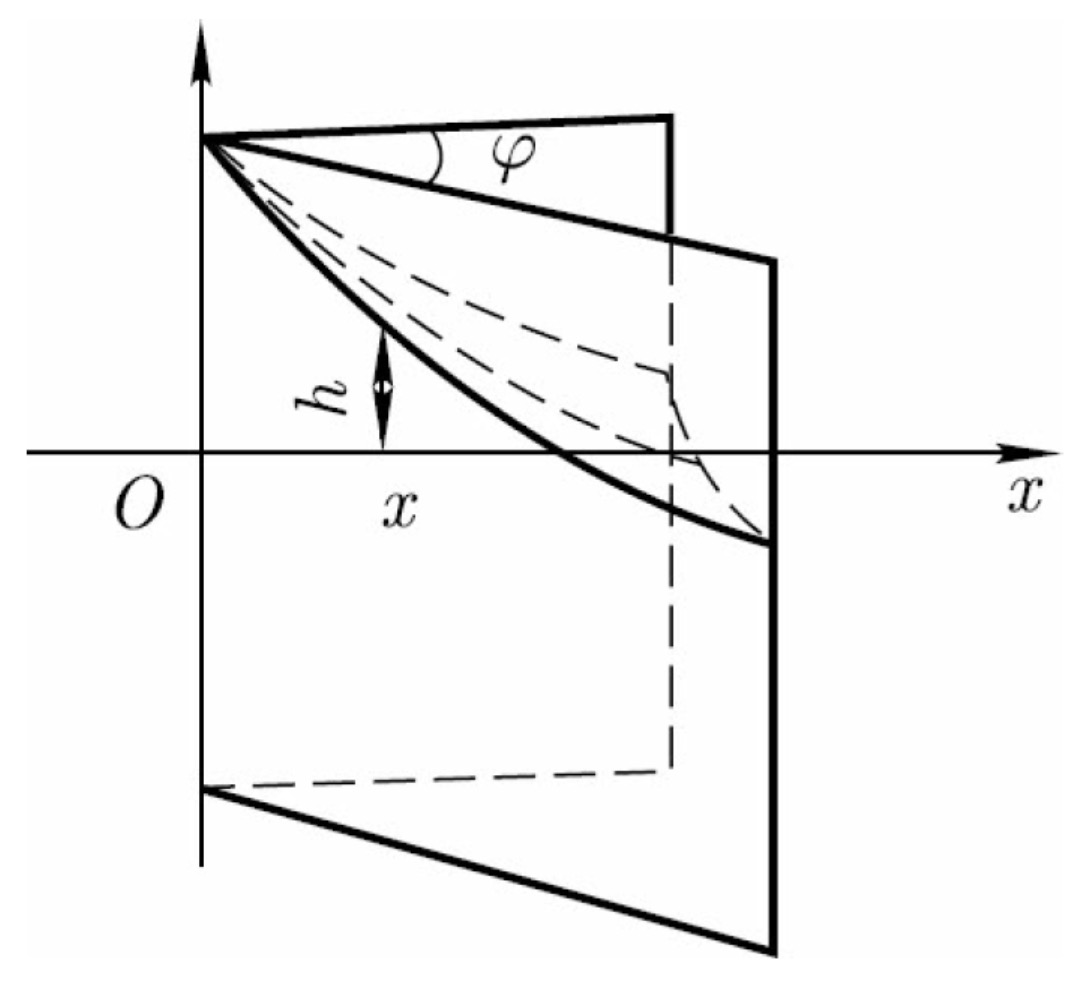
\includegraphics[width=0.4\textwidth]{parallel_plates_capillary.png}
\caption{两平行板与相交板间的毛细液面}
\label{fig:parallel_plates}
\end{figure}

% ============================================================
% 新增内容：第六章（液体部分）习题解答
% ============================================================
\subsection{第六章习题解答}
\subsubsection{题 6.4}

\textbf{题目}：在面积为 $20\ \mathrm{km^2}$ 的湖面上，下了一场 $50\ \mathrm{mm}$ 的大雨。如果雨滴半径为 $2\ \mathrm{mm}$，温度近似保持不变，水的表面张力系数为 $7.3\times 10^{-2}\ \mathrm{N/m}$，试确定该下雨过程中释放出的能量。

\begin{thoughts}
  使用表面能公式$\Delta S = \sigma \Delta S$
\end{thoughts}

\textbf{解答}：

记湖面的面积为 $S$，下雨使湖面的升高量为 $h$，雨滴的总数目为 $N$，雨滴的半径为 $r$，水的表面张力系数为 $\sigma$。由于雨滴落到湖面后，原湖面碎裂，并形成新的湖面，依题意，湖面面积不变，因此所有雨滴的表面积的改变量为
\[
\Delta A=4\pi r^2 N-S.
\]
于是雨水本身表面积变化而释放的能量为
\[
\Delta E=\sigma\cdot(4\pi r^2 N-S).
\]

依题意，雨滴的个数可以由雨滴的半径和所下雨水的体积表示为
\[
N=\frac{hS}{\dfrac{4}{3}\pi r^3},
\]
于是
\[
\Delta E=\sigma\cdot\left(\frac{3hS}{r}-S\right)
=\sigma\cdot S\left(\frac{3h}{r}-1\right).
\]

将已知数据 $S=20\times 10^6\ \mathrm{m^2}$，$h=50\times 10^{-3}\ \mathrm{m}$，$r=2\times 10^{-3}\ \mathrm{m}$，$\sigma=7.3\times 10^{-2}\ \mathrm{N/m}$ 代入：
\[
\Delta E=(7.3\times 10^{-2})\times\left[\frac{3\times(50\times 10^{-3})\times(20\times 10^6)}{2\times 10^{-3}}-(20\times 10^6)\right]
\approx 1.08\times 10^{8}\ \mathrm{J}.
\]

\[
\boxed{\Delta E\approx 1.08\times 10^{8}\ \mathrm{J}}
\]

\textbf{附注}：如果认为雨滴落到湖面后，其表面完全碎裂，而湖面原来就有，则所有雨滴的表面积的改变量为 $\Delta A=4\pi r^2 N$（即不能减去 $S$）。在这种情况下，得到 $\Delta E\approx 1.095\times 10^{8}\ \mathrm{J}$。

\subsubsection{题 6.9}

\textbf{题目}：两个表面张力系数都为 $\sigma$、半径分别为 $R_1,R_2$ 的肥皂泡，在相同的大气中，等温地合并成一个半径为 $R$ 的肥皂泡。试证明：如果泡内的气体可以近似为理想气体，则泡外的大气压强为
\[
p=\frac{4\sigma\bigl(R^2-R_1^2-R_2^2\bigr)}{R_1^3+R_2^3-R^3}.
\]

\begin{thoughts}
  用理想气体状态方程和自由能能量守恒进行求解
\end{thoughts}

\textbf{证明}：

记合并前两肥皂泡的半径分别为 $R_1,R_2$，其中包含的气体的物质的量分别为 $\nu_1,\nu_2$，泡内气体的压强分别为 $p_{i1},p_{i2}$。合并后的肥皂泡的半径为 $R$，其中包含的气体的物质的量为 $\nu$，泡内气体的压强为 $p_i$，泡外的大气压强为 $p$，温度为 $T$。

由弯曲液面内外压强差的拉普拉斯公式知，肥皂泡有内外两个表面，故
\[
p_{i1}=p+\frac{4\sigma}{R_1},\qquad
p_{i2}=p+\frac{4\sigma}{R_2},\qquad
p_i=p+\frac{4\sigma}{R}.
\]

另一方面，假设肥皂泡内的气体可近似为理想气体，由理想气体状态方程 $pV=\nu RT$，得
\[
\left(p+\frac{4\sigma}{R_1}\right)\frac{4}{3}\pi R_1^3=\nu_1 RT,\qquad
\left(p+\frac{4\sigma}{R_2}\right)\frac{4}{3}\pi R_2^3=\nu_2 RT,\qquad
\left(p+\frac{4\sigma}{R}\right)\frac{4}{3}\pi R^3=\nu RT.
\]

由合并过程中物质的量保持不变，即 $\nu=\nu_1+\nu_2$，知
\[
\left(p+\frac{4\sigma}{R_1}\right)R_1^3+\left(p+\frac{4\sigma}{R_2}\right)R_2^3
=\left(p+\frac{4\sigma}{R}\right)R^3.
\]

展开整理得
\[
p\bigl(R_1^3+R_2^3-R^3\bigr)+4\sigma\bigl(R_1^2+R_2^2-R^2\bigr)=0.
\]

解之得
\[
\boxed{p=\frac{4\sigma\bigl(R^2-R_1^2-R_2^2\bigr)}{R_1^3+R_2^3-R^3}}
\]

% [插图：题 6.9 两个肥皂泡合并示意图]
\begin{figure}[htbp]
  \centering
  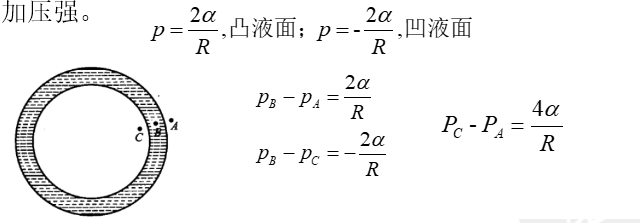
\includegraphics[width=0.7\textwidth]{6_9.png}
  \caption{题 6.9 肥皂泡合并示意图}
  \label{fig:6_9}
\end{figure}


\subsubsection{题 6.12}

\textbf{题目}：利用如题 6.12 图所示的检验弯曲液面内外压强差的拉普拉斯公式的实验装置，在其两端吹肥皂泡。
\begin{enumerate}
  \item[(1)] 试证明：在肥皂泡的形状小于半球的情况下，吹成的肥皂泡是稳定的；如果吹成的肥皂泡的形状大于半球，则肥皂泡不稳定。
  \item[(2)] 如果装置中两管的管口直径都为 $4\ \mathrm{mm}$，吹气停止时形成的都是直径为 $5\ \mathrm{mm}$ 的大于半球的肥皂泡。假设因肥皂膜的位置移动引起的泡内空气的密度的改变可以忽略不计，试确定稳定的肥皂泡的状态。
\end{enumerate}

\begin{thoughts}
  考虑一个微扰使半径增大，当小于半球时肥皂泡倾向于回到原有状态，大于半球时肥皂泡会继续增大直至破裂\\
  由于上述条件，所以我们假设最后状态时一个大于半球一个小于半球，且二者曲率半径相等，故此时二者拼成一个球体，根据体积守恒即可求解，注意球冠的体积是$$V=\pi h^2 (R-\frac{h}{3})$$
\end{thoughts}

% [插图：题 6.12 实验装置示意图]
\begin{figure}[htbp]
  \centering
  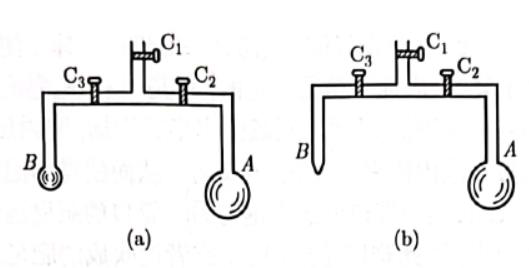
\includegraphics[width=0.6\textwidth]{6_12.png}
  \caption{题 6.12 检验弯曲液面压强差实验装置示意图}
  \label{fig:6_12}
\end{figure}

\textbf{解答}：

(1) 记肥皂泡的曲率半径为 $R$，肥皂泡外的大气压强为 $p_0$，肥皂膜的表面张力系数为 $\sigma$。由弯曲液面内外压强差的拉普拉斯公式知，肥皂泡内气体的压强为
\[
p_i=p_0+\frac{4\sigma}{R}.
\]

显然，$p_i$ 随 $R$ 增大而减小。

记管口的半径为 $R_t$。由几何知识知，当管口的肥皂泡由小于半球状胀大到半球状时，其曲率半径不断减小，$R-R_t$ 由大于 $0$ 的方向趋于 $0$，从而 $p_i$ 逐渐增大至 $p_0+\dfrac{4\sigma}{R_t}$；而当半球状继续胀大时，其曲率半径不断增大，$R-R_t$ 由 $0$ 逐渐增大，从而 $p_i$ 由 $p_0+\dfrac{4\sigma}{R_t}$ 逐渐减小。

对于题 6.12 图所示的装置，记两管口的半径分别为 $R_{t1},R_{t2}$。显然只有当两肥皂泡的曲率半径 $R_1,R_2$ 相同时，两肥皂泡内气体的压强才相同，从而实现稳定。

如果两肥皂泡的形状小于半球，一旦由于某种扰动使其中之一（记之为 1）略微缩小（或增大），则相应的曲率半径即增大（或减小），此泡内的压强 $p_{i1}=p_0+\dfrac{4\sigma}{R_{i1}}$ 便减小（或增大），于是，就由另一泡（记之为 2）来补充气体（或向另一泡流去气体），使得该泡的形状再趋于复原，因此平衡是稳定的。

但是，当两肥皂泡大于半球状时，一旦某一泡略为胀大，则其曲率半径增加，泡内压强减小，有气体从另一泡内流来，另一泡则缩小，从而使得两泡的大小相差越来越大，直到一管口的肥皂泡与另一管口的肥皂泡的曲率半径相等时为止，因此难以达到稳定，或者说吹成的肥皂泡是不稳定的。

(2) 依题意，两肥皂泡的初始状态的曲率半径 $R_{i1}=R_{i2}=R_i$（直径 $5\ \mathrm{mm}$，故 $R_i=2.5\ \mathrm{mm}$），且管口半径 $R_t=2\ \mathrm{mm}$，呈大于半球状。由第 (1) 问的解答知，它们的这一都大于半球状的初始平衡是不稳定的。因此，两肥皂泡的大小都将发生变化，直至它们的曲率半径再相等时为止。

记经过自发演化达到的稳定肥皂泡的曲率半径为 $R_s$，但一个大于半球状，另一个小于半球状，它们的体积之和恰好是半径为 $R_s$ 的球的体积。初始的肥皂泡的体积为 $V$，弯管内气体的体积为 $V_0$。根据系统的质量守恒（等温过程，且密度改变可忽略），有
\[
(V_0+2V)\cdot\frac{\mu}{RT}=\left(V_0+\frac{4}{3}\pi R_s^3\right)\cdot\frac{\mu}{RT}.
\]
（其中 $\mu$ 为摩尔质量，这里利用了 $p\approx p_0$ 近似。）

于是
\[
\frac{4}{3}\pi R_s^3=2V.
\]

由几何知识知，对于半径为 $R_i$、管口外凸出球冠的高度 $h$ 大于半球的肥皂泡，其体积为
\[
V=\pi h^2\left(R_i-\frac{h}{3}\right),
\qquad h=R_i+\sqrt{R_i^2-R_t^2}.
\]

将已知数据 $R_t=2\ \mathrm{mm}$，$R_i=2.5\ \mathrm{mm}$ 代入计算 $V$，再由 $R_s=\left(\dfrac{3}{2\pi}V\right)^{1/3}$ 得
\[
\boxed{R_s\approx 3.04\ \mathrm{mm}}.
\]

相应地，
\[
h_1=R_s+\sqrt{R_s^2-R_t^2}=3.04+\sqrt{3.04^2-2^2}\approx 5.33\ \mathrm{mm},
\]
\[
h_2=2R_s-h_1\approx 0.75\ \mathrm{mm}.
\]

即稳定时，一个肥皂泡的球冠高度约为 $5.33\ \mathrm{mm}$（大于半球），另一个约为 $0.75\ \mathrm{mm}$（小于半球），两者的曲率半径均为 $3.04\ \mathrm{mm}$。



\subsubsection{题 6.16}

\textbf{题目}：对在空气中匀速下落的雨滴测得其上下两端的间距为 $d=2\ \mathrm{mm}$。试确定该雨滴上下两端处的曲率半径之差。

\begin{thoughts}
  上下压强相差$\rho gh$，曲率半径近似相等
\end{thoughts}

\textbf{解答}：

记雨滴上端附近的曲率半径为 $R_u$，雨滴内上端附近的压强为 $p_u$；雨滴下端附近的曲率半径为 $R_d$，雨滴内下端附近的压强为 $p_d$；雨滴外的大气压强为 $p_0$，水与空气之间的表面张力系数为 $\sigma$。

由弯曲液面内外压强差的拉普拉斯公式知（凸液面）：
\[
p_u-p_0=\frac{2\sigma}{R_u},\qquad
p_d-p_0=\frac{2\sigma}{R_d}.
\]

依题意，雨滴匀速下落，其内部压强差由重力引起：
\[
p_d=p_u+\rho gd.
\]

于是
\[
\rho gd=p_d-p_u=(p_d-p_0)-(p_u-p_0)=2\sigma\left(\frac{1}{R_d}-\frac{1}{R_u}\right)
=\frac{2\sigma(R_u-R_d)}{R_u R_d}.
\]

故
\[
R_u-R_d=\frac{\rho gd\,R_u R_d}{2\sigma}.
\]

因为 $R_u\approx R_d\approx \dfrac{d}{2}$，则上式可近似为
\[
R_u-R_d\approx\frac{\rho gd^3}{8\sigma}.
\]

将已知数据代入（$\rho=1\times 10^3\ \mathrm{kg/m^3}$，$g=9.8\ \mathrm{m/s^2}$，$d=2\times 10^{-3}\ \mathrm{m}$，$\sigma=7.3\times 10^{-2}\ \mathrm{N/m}$）：
\[
R_u-R_d\approx\frac{(1\times 10^3)\times 9.8\times(2\times 10^{-3})^3}{8\times 7.3\times 10^{-2}}
\approx 1.34\times 10^{-4}\ \mathrm{m}=0.134\ \mathrm{mm}.
\]

\[
\boxed{R_u-R_d\approx 0.134\ \mathrm{mm}}
\]

\textbf{附注}：由于雨滴上下两端处的曲率半径之差大于零，即上端附近的曲率半径大于下端附近的曲率半径，也就是说，上端附近相对于下端附近较平坦。由此知，雨滴近似呈倒梨子形。

% [插图：题 6.16 雨滴形状及曲率半径示意图]
\begin{figure}[htbp]
  \centering
  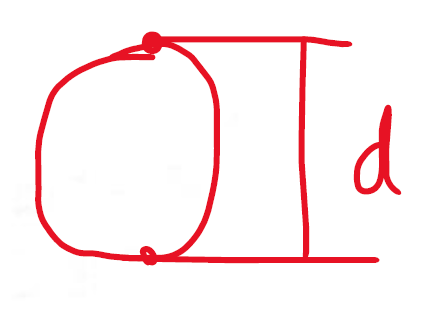
\includegraphics[width=0.3\textwidth]{6_16.png}
  \caption{题 6.16 雨滴上下端曲率半径示意图}
  \label{fig:6_16}
\end{figure}


\subsubsection{题 6.21}

\textbf{题目}：在内半径为 $R_1=2\times 10^{-2}\ \mathrm{m}$ 的玻璃管中插入一根半径为 $R_2=1.5\times 10^{-2}\ \mathrm{m}$ 的玻璃棒，并使玻璃棒与玻璃管同轴。实验测得水的密度为 $1\times 10^3\ \mathrm{kg/m^3}$，水与玻璃间的表面张力系数为 $7.3\times 10^{-2}\ \mathrm{N/m}$，水与玻璃间的接触角为 $0^{\circ}$，试确定水在玻璃管与玻璃棒之间的缝隙中上升的高度。

\begin{thoughts}
  核心公式推导
  $$\boxed{h = \frac{2\sigma \cos\theta}{\rho g d}}$$
\end{thoughts}
\textbf{解答}：

依题意，在任意的同轴同径向处的水面都可以近似为两平行板之间的水面。因为表面张力的作用，两平行板之间的液面呈柱面，柱形液面的轴线与板面平行，所以该玻璃管内表面与玻璃棒外表面之间的液面呈中间凹陷的环形。

对于任意的同轴同径向处的柱形液面，因为其两个正截口中的一个是与柱面的轴线垂直的圆弧（即包含玻璃管和玻璃棒的轴线的竖直平面内的圆弧），另一个是与板面平行的直线段（即与上述圆弧形截面垂直的直线段），则其曲率半径可以分别记为 $R,\infty$。

由弯曲液面内外压强差的拉普拉斯公式知，液面之外的压强为 $p_0$，液面下紧靠液面处的压强为 $p_l$，液体的表面张力系数为 $\sigma$，则该液面内外的压强差为
\[
p_l-p_0=-\frac{\sigma}{R}.
\]
（凹液面，曲率中心在液体外部。）

两板之间的液面相对于不在两平行板之间的液面的高度差为 $h$，则不在两平行板之间的液面下紧靠液面处的压强为大气压强 $p_0$，由液柱稳定的力学平衡条件知
\[
p_0=p_l+\rho gh.
\]

于是有
\[
h=\frac{\sigma}{\rho g R}.
\]

记两平行板之间的间距为 $d$，水与玻璃间的接触角为 $\theta$，则前述圆弧形液面的曲率半径 $R$ 与两平行板之间的间距 $d$ 的关系为
\[
R=\frac{d/2}{\cos\theta}.
\]

因此
\[
h=\frac{2\sigma\cos\theta}{\rho g d}.
\]

依题意，这里所述的两平行板之间的间距为同一径向上玻璃管的内缘与玻璃棒的外缘之间的距离，即有 $d=R_1-R_2$，所以
\[
h=\frac{2\sigma\cos\theta}{\rho g(R_1-R_2)}.
\]

将已知数据代入：
\[
h=\frac{2\times(7.3\times 10^{-2})\times\cos 0^{\circ}}{(1\times 10^3)\times 9.8\times(2\times 10^{-2}-1.5\times 10^{-2})}
\approx 2.98\times 10^{-3}\ \mathrm{m}.
\]

\[
\boxed{h\approx 2.98\times 10^{-3}\ \mathrm{m}}
\]

% [插图：题 6.21 同轴玻璃管与玻璃棒间液面示意图]
\begin{figure}[htbp]
  \centering
  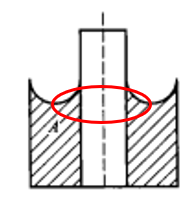
\includegraphics[width=0.4\textwidth]{6_21.png}
  \caption{题 6.21 同轴管棒间毛细上升示意图}
  \label{fig:6_21}
\end{figure}


\subsubsection{题 6.22}

\textbf{题目}：将一根一端封闭的玻璃管开口朝下竖直插入水中，如果玻璃管的内直径为 $d=2\times 10^{-5}\ \mathrm{m}$，长为 $l=0.2\ \mathrm{m}$，水与空气间的表面张力系数为 $\sigma=7.3\times 10^{-2}\ \mathrm{N/m}$，水与玻璃的接触角为 $\theta=0^{\circ}$，大气压强为 $p_0=1.013\times 10^{5}\ \mathrm{Pa}$，试确定插入水面下的那一段玻璃管的长度应为多少，才能使管内外的水面一样高？

\begin{thoughts}
  核心公式注意$$P_1 = P_0 - \boxed{\frac{4\sigma}{d}}$$
  用理想状态方程和$h=0$列出等式
\end{thoughts}

\textbf{解答}：

记插入水面下的那一段玻璃管的长度为 $h$，则平衡时封闭在玻璃管中的空气柱的长度为 $l-h$。观测到管内外的水面高度一样，表明管内液面下侧紧靠液面处的压强与管外平直液面下侧紧靠液面处的压强相同，都为大气压强 $p_0$。

依题意，细管内的水面呈与管壁接触角为 $0^{\circ}$ 的弯曲形状，由弯曲液面内外压强差的拉普拉斯公式知，封闭在玻璃管内的空气的压强为
\[
p_c=p_0+\frac{2\sigma}{R}=p_0+\frac{4\sigma}{d}.
\]
（凹液面，曲率半径 $R=d/2$。）

依题意，该压强为将一定量的空气从压强为 $p_0$、体积为 $\pi\left(\dfrac{d}{2}\right)^2 l$ 的初始状态等温压缩到体积为 $\pi\left(\dfrac{d}{2}\right)^2(l-h)$ 的状态时的压强。于是，由等温过程方程 $pV=\text{常量}$ 得
\[
p_0\pi\left(\frac{d}{2}\right)^2 l=\left(p_0+\frac{4\sigma}{d}\right)\pi\left(\frac{d}{2}\right)^2(l-h).
\]

解之得
\[
h=\frac{4\sigma}{p_0 d+4\sigma}\,l.
\]

将已知数据代入：
\[
h=\frac{4\times(7.3\times 10^{-2})}{(1.013\times 10^{5})\times(2\times 10^{-5})+4\times(7.3\times 10^{-2})}\times 0.2
\approx 2.52\times 10^{-2}\ \mathrm{m}.
\]

\[
\boxed{h\approx 2.52\times 10^{-2}\ \mathrm{m}}
\]

% [插图：题 6.22 封闭玻璃管插入水中示意图]
\begin{figure}[htbp]
  \centering
  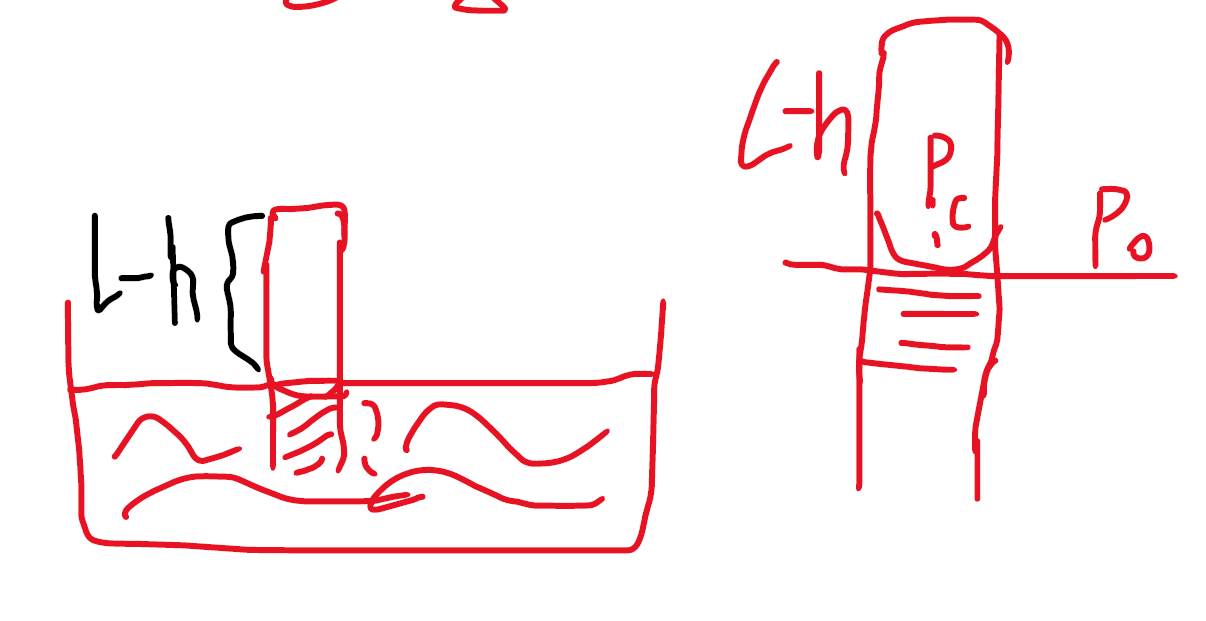
\includegraphics[width=0.45\textwidth]{6_22.png}
  \caption{题 6.22 封闭玻璃管内外水面等高示意图}
  \label{fig:6_22}
\end{figure}


\subsubsection{题 6.23}

\textbf{题目}：将一充满水银的气压计下端浸在一个广阔的盛有水银的容器中时，读数为 $p=0.95\times 10^{5}\ \mathrm{Pa}$。已知毛细管的直径为 $d=2\times 10^{-3}\ \mathrm{m}$，接触角为 $\theta=\pi$，水银的表面张力系数为 $\sigma=0.49\ \mathrm{N/m}$，密度为 $\rho=13.6\times 10^{3}\ \mathrm{kg/m^3}$。
\begin{enumerate}
  \item[(1)] 试确定水银柱的高度。
  \item[(2)] 考虑到毛细现象后，真正的大气压强为多大？
  \item[(3)] 如果允许误差为 $0.1\%$，毛细管直径所能允许的最小值为多大？
\end{enumerate}

\begin{thoughts}
  水银气压计通过水银高度确定气压，但由于不浸润现象结果偏低，即上端近水银处的压强大于0
\end{thoughts}

\textbf{解答}：

(1) 记气压计显示的压强为 $p$，水银柱高度为 $h$，水银密度为 $\rho$，重力加速度为 $g$，则液体内部压强与其深度的关系为
\[
p=\rho gh.
\]
因此
\[
h=\frac{p}{\rho g}=\frac{0.95\times 10^{5}}{(13.6\times 10^{3})\times 9.8}\approx 0.713\ \mathrm{m}=713\ \mathrm{mm}.
\]

(2) 记气压计中毛细管内液面外侧紧靠液面处的压强为 $p_1$（即真空侧，近似为 $0$），管内液面内侧紧靠液面处的压强为 $p_l$，管外平直液面下侧紧靠液面处的压强（大气压强）为 $p_0$。水银的密度为 $\rho$，那么高度为 $h$ 的水银柱下侧（即与管外平直液面同高处）的压强为
\[
p_h=p_l+\rho gh.
\]

另一方面，依题意知，毛细管内的水银面呈与管壁接触角为 $\pi$ 的弯曲形状（凸液面），因其两个正截口都是与管的半径相同的半圆，记该半径为 $R$，管的直径为 $d$，由弯曲液面内外压强差的拉普拉斯公式知，毛细管内水银面下侧紧靠表面处的压强为
\[
p_l=p_1+\frac{2\sigma}{R}=\frac{4\sigma}{d}.
\]
（凸液面，曲率半径 $R=d/2$，且 $p_1\approx 0$。）

于是有
\[
p_h=\frac{4\sigma}{d}+\rho gh.
\]

考虑水银柱稳定的力学平衡条件知，该压强即为管外平直液面下侧紧靠液面处的压强，亦即大气压强 $p_0$，因此
\[
p_0=p+\frac{4\sigma}{d}.
\]

将已知数据代入：
\[
p_0=0.95\times 10^{5}+\frac{4\times 0.49}{2\times 10^{-3}}
=0.95\times 10^{5}+980
=0.9598\times 10^{5}\ \mathrm{Pa}.
\]

\[
\boxed{p_0\approx 0.9598\times 10^{5}\ \mathrm{Pa}}
\]

(3) 依题意，仅考虑由毛细管直径引起的测量误差，由 (2) 式知，对毛细管直径的测量误差与对大气压强的测量误差之间的关系为
\[
\Delta p_0=-\frac{4\sigma\,\Delta d}{d^2}.
\]

相对误差为
\[
\left|\frac{\Delta p_0}{p_0}\right|=\left|\frac{4\sigma\,\Delta d}{d^2 p_0}\right|.
\]

因此有
\[
|\Delta d|=\frac{d^2}{4\sigma}\,p_0\left|\frac{\Delta p_0}{p_0}\right|.
\]

将已知数据代入（允许误差 $0.1\%=10^{-3}$）：
\[
|\Delta d|=\frac{(2\times 10^{-3})^2}{4\times 0.49}\times(0.9598\times 10^{5})\times 10^{-3}
\approx 1.96\times 10^{-4}\ \mathrm{m}.
\]

那么，
\[
d_{\min}=d-|\Delta d|=2\times 10^{-3}-1.96\times 10^{-4}=1.804\times 10^{-3}\ \mathrm{m}.
\]

\[
\boxed{d_{\min}\approx 1.80\times 10^{-3}\ \mathrm{m}}
\]

% [插图：题 6.23 水银气压计毛细现象示意图]
\begin{figure}[htbp]
  \centering
  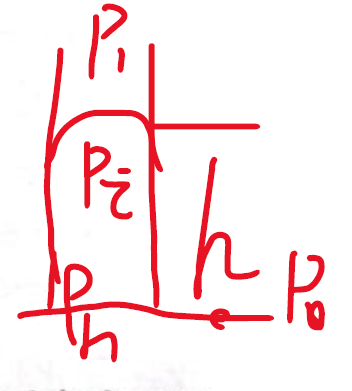
\includegraphics[width=0.3\textwidth]{6_23.png}
  \caption{题 6.23 水银气压计毛细修正示意图}
  \label{fig:6_23}
\end{figure}


\subsubsection{题 6.29}

\textbf{题目}：在一根两端开口的毛细管中滴入一滴水后将它竖直放置，若这滴水在毛细管中分别形成长为 (1) $2.00\ \mathrm{cm}$，(2) $4.00\ \mathrm{cm}$，(3) $2.98\ \mathrm{cm}$ 的水柱。毛细管的内直径为 $1\ \mathrm{mm}$，并且能够完全被水润湿，水的表面张力系数为 $0.073\ \mathrm{N/m}$，试确定在上述三种情况下，水柱的上、下液面各呈什么样的形状。

\begin{thoughts}
  实际上是比较液体高度压强和因浸润现象产生压强差的大小关系
\end{thoughts}

\textbf{解答}：

记大气压强为 $p_0$，毛细管直径为 $d$。因为水可以完全润湿毛细管，记液体上表面外侧紧靠液面处的压强为 $p_A=p_0$，液体上表面内侧紧靠液面处的压强为 $p_B$，液体下表面内侧紧靠液面处的压强为 $p_C$，液体下表面外侧紧靠液面处的压强为 $p_D=p_0$。

由弯曲液面内外压强差的拉普拉斯公式知，对于液体上表面（凹液面，接触角 $0^{\circ}$），有
\[
p_B=p_A-\frac{2\sigma}{r}=p_0-\frac{4\sigma}{d}.
\]

所以，液体上表面一定都是上凹的，即凸向液体内部的。

对于液体下表面，同理知
\[
p_C=p_B+\rho gh=p_0-\frac{4\sigma}{d}+\rho gh.
\]

因为 $p_D=p_A=p_0$，则
\[
p_D-p_C=\frac{4\sigma}{d}-\rho gh.
\]

这表明：
\begin{itemize}
  \item 若 $\rho gh<\dfrac{4\sigma}{d}$，则 $p_D-p_C>0$，液体下表面凹向液体内部，即是上凸的（凸向下方气体）；
  \item 若 $\rho gh=\dfrac{4\sigma}{d}$，则 $p_D-p_C=0$，液体下表面是平直的；
  \item 若 $\rho gh>\dfrac{4\sigma}{d}$，则 $p_D-p_C<0$，液体下表面凸向液体外部，即是上凹的（凹向下方气体）。
\end{itemize}

对直径 $d=1\ \mathrm{mm}$ 的毛细管，有
\[
\frac{4\sigma}{d}=\frac{4\times 0.073}{1\times 10^{-3}}=292\ \mathrm{N/m^2}.
\]

计算三种情况下的 $\rho gh$：
\begin{itemize}
  \item 当 $h=2.00\ \mathrm{cm}$ 时，$\rho gh=1000\times 9.8\times 0.02=196\ \mathrm{N/m^2}<\dfrac{4\sigma}{d}$；
  \item 当 $h=4.00\ \mathrm{cm}$ 时，$\rho gh=1000\times 9.8\times 0.04=392\ \mathrm{N/m^2}>\dfrac{4\sigma}{d}$；
  \item 当 $h=2.98\ \mathrm{cm}$ 时，$\rho gh=1000\times 9.8\times 0.0298\approx 292\ \mathrm{N/m^2}=\dfrac{4\sigma}{d}$。
\end{itemize}

所以：
\begin{itemize}
  \item 当水柱长为 $2.00\ \mathrm{cm}$ 时，\textbf{其上下表面都凹向液体内部}（上表面凹向上，下表面凸向下）；
  \item 当水柱长为 $4.00\ \mathrm{cm}$ 时，\textbf{其上表面凹向液体内部，下表面凸向液体外部}（上表面凹向上，下表面凹向下）；
  \item 当水柱长为 $2.98\ \mathrm{cm}$ 时，\textbf{其上表面凹向液体内部，下表面平直}。
\end{itemize}

% [插图：题 6.29 毛细管中水柱液面形状示意图]
\begin{figure}[htbp]
  \centering
  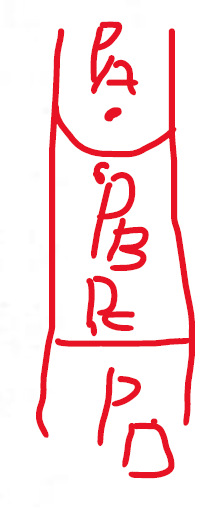
\includegraphics[width=0.25\textwidth]{6_29.png}
  \caption{题 6.29 毛细管中水柱上下液面形状示意图}
  \label{fig:6_29}
\end{figure}


\subsubsection{题 6.33}

\textbf{题目}：如果农作物、花草灌木及树木中传输水分及营养物质的导管是内半径为 $5\ \mu\mathrm{m}$ 的细圆柱形管，水分及营养物质的表面张力系数为 $9\times 10^{-2}\ \mathrm{N/m}$，密度为 $1.1\times 10^{3}\ \mathrm{kg/m^3}$，地面及其附近的重力加速度为 $9.8\ \mathrm{m/s^2}$，试通过定量计算说明水分及营养物质在农作物及花草灌木中传输的机制可能主要是毛细现象，而在高大的树木中一定还有其他机制。

\textbf{解答}：

依题意，该问题为竖直细管内的毛细现象问题。地面相当于很大的容器内的平直液面，水分及营养物质在农作物及花草灌木等中传输的高度就是毛细管中液面上升的高度。根据液柱稳定的力学平衡条件和弯曲液面内外压强差的拉普拉斯公式知，密度为 $\rho$、表面张力系数为 $\sigma$、与管壁间的接触角为 $\theta$ 的包含水分及营养物质的液体在内半径为 $R$ 的细管内的上升高度为
\[
h=\frac{2\sigma\cos\theta}{\rho gR}.
\]

显然，在包含水分及营养物质的液体的性质和导管材料的性质确定的情况下，接触角 $\theta=0^{\circ}$ 时，上述 $h$ 取极大值。

将已知数据代入上式：
\[
h_{\max}=\frac{2\sigma}{\rho gR}
=\frac{2\times(9\times 10^{-2})}{(1.1\times 10^{3})\times 9.8\times(5\times 10^{-6})}
\approx 3.34\ \mathrm{m}.
\]

\[
\boxed{h_{\max}\approx 3.34\ \mathrm{m}}
\]

这一具体计算结果表明，包含水分及营养物质的液体在内半径为 $5\ \mu\mathrm{m}$ 的导管中向上传输的最大高度约为 $3.34\ \mathrm{m}$，大于通常的农作物及花草灌木的高度。那么包含水分及营养物质的液体可以传输到农作物及花草灌木的顶端，因此水分及营养物质在农作物及花草灌木中传输的机制可能主要是毛细现象。

由于高大树木的高度显然大于上述包含水分及营养物质的液体能够向上传输的最大高度，那么根据毛细现象输送水分及营养物质的机制，包含水分及营养物质的液体不能传输到高大树木的顶端。事实上，高大树木仍然枝繁叶茂，这一事实表明，包含水分及营养物质的液体一定能传输到高大树木的顶端，因此高大树木中一定还有其他机制来传输水分及营养物质。

% [插图：题 6.33 植物导管毛细现象示意图]
\begin{figure}[htbp]
  \centering
  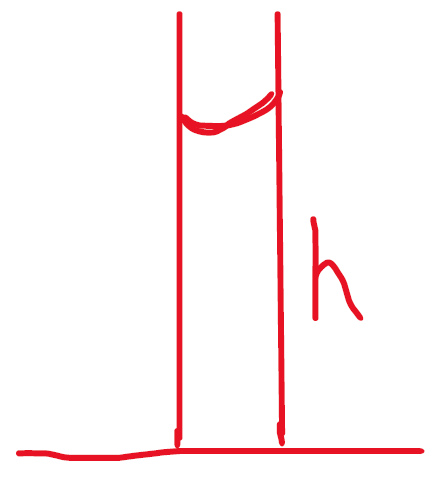
\includegraphics[width=0.35\textwidth]{6_33.png}
  \caption{题 6.33 植物导管中水分传输示意图}
  \label{fig:6_33}
\end{figure}

\newpage
% ============================================================
\section{第七章：单元系统的复相平衡与相变}
% ============================================================

\subsection{相、相变及相平衡的概念}

\subsubsection{相的概念与相稳定条件}

\paragraph{相的定义}
在没有外界影响下，被一定边界包围的，具有确定并且均匀的物理和化学性质的一个系统（或系统的一部分）所处的状态，称为物质的一个\textbf{相}。

\paragraph{相稳定条件}
一般情况，平衡态稳定条件可以表示为：
\[
\left(\frac{\partial\mu}{\partial n}\right)_{T,p}>0,\qquad
C_V>0,\qquad
\kappa_S\ge 0
\]
其中 $\mu$ 为化学势，$C_V$ 为定容热容，$\kappa_S$ 为绝热压缩系数。

\subsubsection{相变及其分类}

物质在压强、温度等外界条件不变的情况下，从一个相转变为另一个相的现象称为\textbf{相变}。相变过程是物质性质的\textbf{突然变化}。

\paragraph{按物理性质变化分类}
\begin{itemize}[leftmargin=2em]
  \item \textbf{一级相变}：相变发生时，两相之间有潜热和体积等跃变。如：液气相变、固液相变。
  \item \textbf{二级相变}：相变发生时，两相之间无潜热和体积跃变，但有热容跃变。如：超导相变、液氦相变。
\end{itemize}

\paragraph{用数学方法分类}
\begin{itemize}[leftmargin=2em]
  \item \textbf{一级相变}：热力学函数连续，但其状态参量的一阶导数不连续。
  \item \textbf{二级相变}：热力学函数及其关于状态参量的一阶导数都连续，但其关于状态参量的二阶导数不连续。
\end{itemize}

\subsubsection{相平衡及相图}

\paragraph{相平衡}
相平衡是一个\textbf{动态平衡}。

\paragraph{相图}
把一物质系统的相、相变及相平衡以其状态参量为变量所作的图示，称为\textbf{相图}（phase diagram）。

% [插图：典型单元系相图 p-T 图，标注固、液、气三相区及汽化曲线、熔解曲线、升华曲线]
\begin{figure}[htbp]
  \centering
  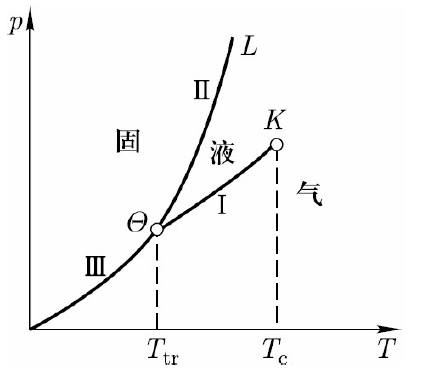
\includegraphics[width=0.5\textwidth]{phase_diagram.png}
  \caption{典型单元系相图（$p$-$T$ 图）}
  \label{fig:phase_diagram}
\end{figure}

\paragraph{相图的关键要素}
\begin{itemize}[leftmargin=2em]
  \item \textbf{汽化曲线}（$I$）：液气两相平衡共存曲线；
  \item \textbf{熔解曲线}（$II$）：固液两相平衡共存曲线；
  \item \textbf{升华曲线}（$III$）：固气两相平衡共存曲线；
  \item \textbf{三相点}（$\Theta$）：三条曲线交点，三相共存；
  \item \textbf{临界点}（$K$）：汽化曲线终点，对应临界温度 $T_c$。
\end{itemize}

\paragraph{临界温度}
在温度低于临界温度 $T_c$ 的情况下，系统可以发生有液气共存状态的一级相变（有摩尔体积突变）；而在 $T_c$ 之上，系统不再有液气共存状态，即不再能发生一级相变。


% ============================================================
\subsection{单元系的复相平衡}
% ============================================================

\subsubsection{单元系复相平衡的条件}

对 $\alpha$ 相和 $\beta$ 相的两相系统，相平衡时两相的化学势相等：
\[
\mu_\alpha(T,p)=\mu_\beta(T,p)
\]

当外界条件发生微小变化时，为保持平衡，有
\[
\mathrm{d}\mu_\alpha=\mathrm{d}\mu_\beta
\]

利用 $\mathrm{d}\mu=-S_m\,\mathrm{d}T+V_m\,\mathrm{d}p$，得
\[
-S_{\alpha,m}\,\mathrm{d}T+V_{\alpha,m}\,\mathrm{d}p
=-S_{\beta,m}\,\mathrm{d}T+V_{\beta,m}\,\mathrm{d}p
\]

整理得相平衡曲线的斜率：
\[
\frac{\mathrm{d}p}{\mathrm{d}T}
=\frac{S_{\beta,m}-S_{\alpha,m}}{V_{\beta,m}-V_{\alpha,m}}
\]

\subsubsection{克拉珀龙方程}

在一级相变中，定义\textbf{摩尔相变潜热}：
\[
\boxed{\Lambda_m=T(S_{\beta,m}-S_{\alpha,m})}
\]

代入上式即得\textbf{克拉珀龙方程}：
\[
\boxed{\frac{\mathrm{d}p}{\mathrm{d}T}
=\frac{\Lambda_m}{T(V_{\beta,m}-V_{\alpha,m})}}
\]

或称为\textbf{克拉珀龙--克劳修斯方程}。

\paragraph{常见物质相变的相平衡曲线特征}
\begin{itemize}[leftmargin=2em]
  \item \textbf{汽化、升华过程}：$V_{\beta,m}>V_{\alpha,m}$，$\Lambda_m>0$，故 $\dfrac{\mathrm{d}p}{\mathrm{d}T}>0$。压强升高，沸点升高。
  \item \textbf{熔解过程（正常物质）}：$V_{\beta,m}>V_{\alpha,m}$（液相体积大于固相），$\dfrac{\mathrm{d}p}{\mathrm{d}T}>0$。压强升高，熔点升高。
  \item \textbf{熔解过程（反常物质，如水）}：$V_{\beta,m}<V_{\alpha,m}$（冰熔解时体积减小），$\dfrac{\mathrm{d}p}{\mathrm{d}T}<0$。压强升高，熔点降低。
\end{itemize}

% [插图：汽化、升华及熔解过程的相平衡曲线示意图]
\begin{figure}[htbp]
  \centering
  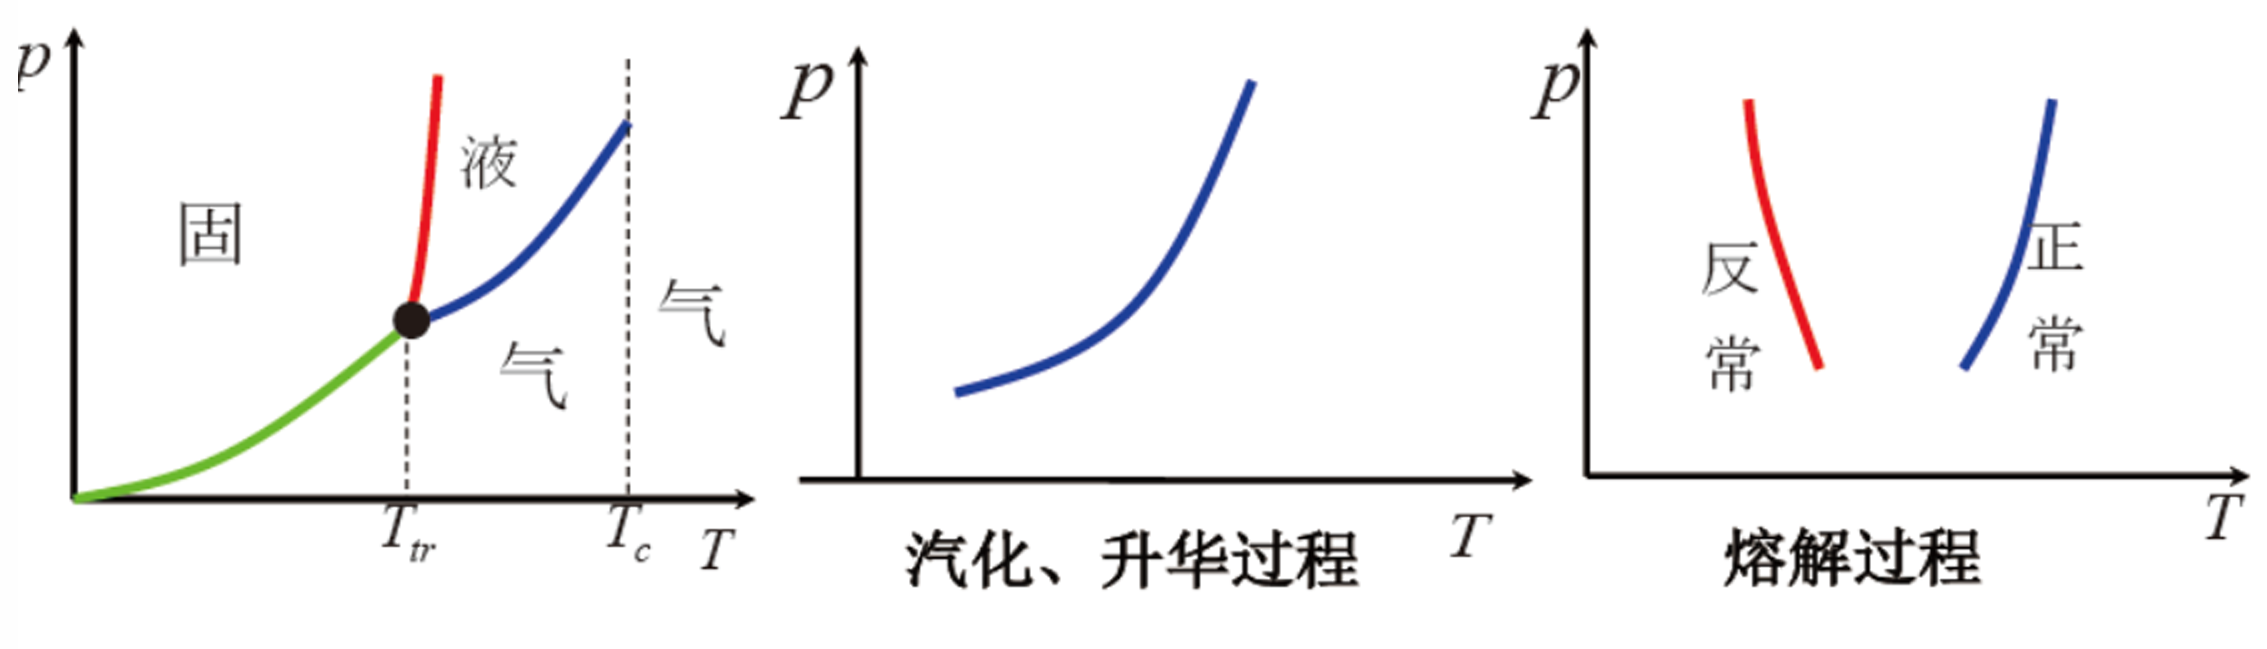
\includegraphics[width=0.8\textwidth]{clapeyron_curves.png}
  \caption{常见物质相变的相平衡曲线}
  \label{fig:clapeyron_curves}
\end{figure}

\subsubsection{相变潜热}

设 $u_1,u_2$ 和 $v_1,v_2$ 分别是 $1$ 相和 $2$ 相的\textbf{单位质量内能}与\textbf{比体积}（单位质量的体积）。

根据热力学第一定律，单位质量物质由 $1$ 相转变为 $2$ 相时，所吸收的相变潜热 $l$ 等于内能增量加上克服恒定外部压强 $p$ 所作的功：
\[
\boxed{l=(u_2-u_1)+p(v_2-v_1)}
\]

其中：
\begin{itemize}[leftmargin=2em]
  \item \textbf{内潜热}：$u_2-u_1$（内能增量）；
  \item \textbf{外潜热}：$p(v_2-v_1)$（对外做功）。
\end{itemize}

又因为焓 $h=u+pv$，故在定压条件下：
\[
\boxed{l=h_2-h_1=\Delta H}
\]

即定压相变潜热等于两相的焓差。

\paragraph{例题（李椿书 P246 例题）}
在外界压强 $p=1\ \mathrm{atm}$ 时，水的沸点为 $100^{\circ}\mathrm{C}$，汽化热 $l=2.26\times 10^6\ \mathrm{J/kg}$。已知此时水蒸气的比体积 $v_2=1.673\ \mathrm{m^3/kg}$，水的比体积 $v_1=1.04\times 10^{-3}\ \mathrm{m^3/kg}$。

\textbf{解}：
外潜热：
\[
p(v_2-v_1)=1.013\times 10^5\times(1.673-0.00104)\approx 1.69\times 10^5\ \mathrm{J/kg}
\]

内潜热：
\[
u_2-u_1=l-p(v_2-v_1)=2.26\times 10^6-1.69\times 10^5\approx 2.09\times 10^6\ \mathrm{J/kg}
\]

\subsubsection{沸腾的定性分析}

\paragraph{沸腾现象}
在一定压强下，加热液体达某一温度时，液体内部和器壁上涌现出大量气泡，整个液体上下翻滚剧烈汽化，称为\textbf{沸腾}，相应温度称为\textbf{沸点}。

\paragraph{沸腾条件}
液体沸腾的条件就是\textbf{饱和蒸气压等于外界压强}：
\[
p_0=p_{\text{外}}
\]

\paragraph{气泡平衡条件}
气泡内压强由两部分组成：泡内气体压强与饱和蒸气压强。平衡时，泡内外压强差满足弯曲液面的附加压强（拉普拉斯公式）：
\[
p_i-p_e=\frac{2\sigma}{r}
\]

其中 $p_i$ 为泡内压强，$p_e$ 为外部液体压强，$r$ 为气泡半径。

温度升高时，饱和蒸气压 $p_0$ 增大，气泡不断胀大。当气泡内部饱和蒸气压等于外界压强时，气泡无法维持平衡而骤然胀大，迅速上升并在液面破裂，形成沸腾。

% [插图：沸腾前后气泡变化示意图]
\begin{figure}[htbp]
  \centering
  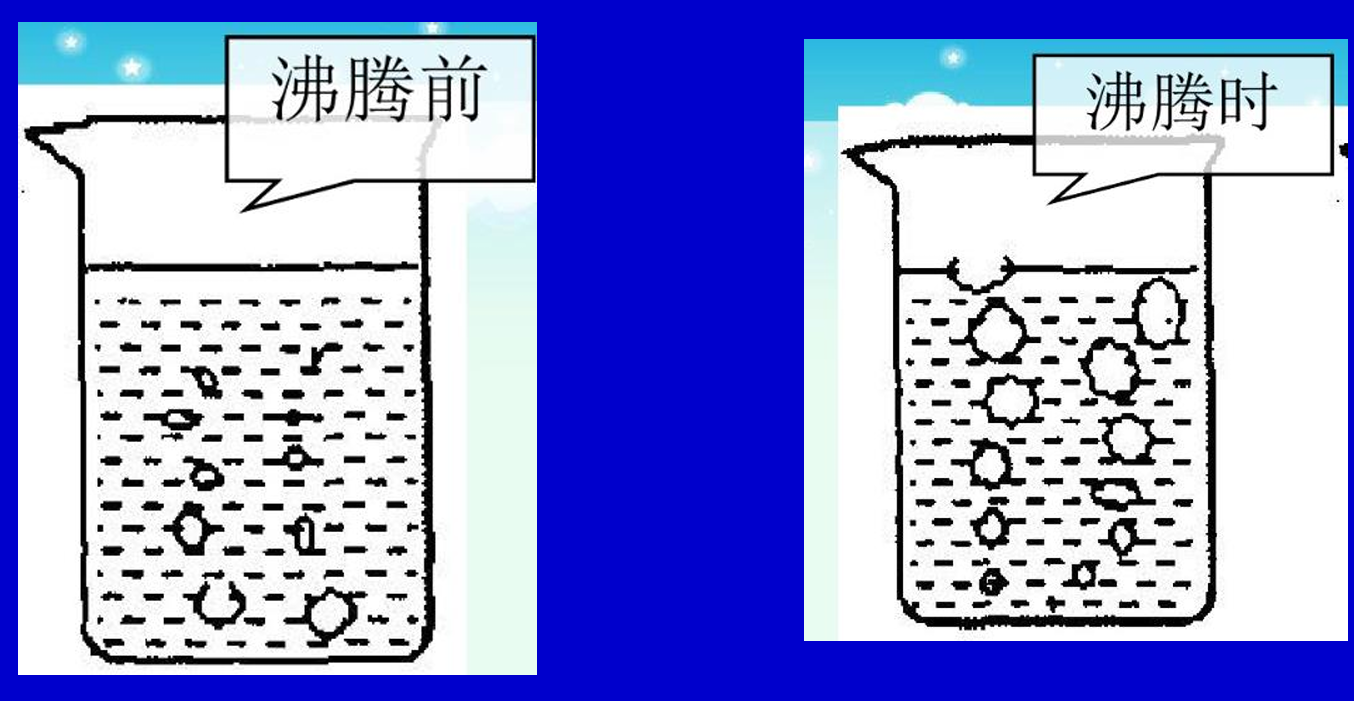
\includegraphics[width=0.6\textwidth]{boiling.png}
  \caption{沸腾时气泡的形成与上升}
  \label{fig:boiling}
\end{figure}

\subsubsection{用克拉珀龙方程说明沸点与熔点}

由克拉珀龙方程：
\[
\frac{\mathrm{d}p}{\mathrm{d}T}=\frac{\Lambda_m}{T(V_{\beta,m}-V_{\alpha,m})}
\]

\paragraph{(1) 液体沸点与压强的关系}
液气相变中，$V_{\beta,m}>V_{\alpha,m}$，$\Lambda_m>0$，故
\[
\frac{\mathrm{d}p}{\mathrm{d}T}>0
\]
\textbf{压强升高，沸点升高}。

\paragraph{(2) 固体熔点与压强的关系}
固液相变中：
\begin{itemize}[leftmargin=2em]
  \item 若 $V_2>V_1$（正常物质），则 $\dfrac{\mathrm{d}p}{\mathrm{d}T}>0$，\textbf{压强升高，熔点升高}；
  \item 若 $V_2<V_1$（反常物质，如水），则 $\dfrac{\mathrm{d}p}{\mathrm{d}T}<0$，\textbf{压强升高，熔点降低}。
\end{itemize}


将一根钢丝跨在冰块上，下面挂一重物。钢丝会逐渐嵌入冰不断下陷，最后钢丝穿过冰块，而冰块并末被切割成两半。\\
因为在钢丝下面的冰受到较大的压力，熔点降低，熔化为水，使钢丝下陷；但已熔化的水在钢丝上面不再受到它的压力，又复凝固

% ============================================================
\subsection{一级相变及其基本特征}
% ============================================================

\subsubsection{常见一级相变概述}

\paragraph{液气相变}
物质由液相转变为气相的过程称为\textbf{汽化}（蒸发、沸腾），吸收\textbf{汽化热}；由气相转变为液相的过程称为\textbf{凝结}，放出\textbf{凝结热}。液气相变达到平衡时，气相蒸气称为\textbf{饱和蒸气}，其压强称为\textbf{饱和蒸气压}。

\paragraph{固液相变}
物质由固相转变为液相的过程称为\textbf{熔解}（熔化），吸收\textbf{熔解热}；从液相转变为固相的过程称为\textbf{凝固}（结晶），放出\textbf{凝固热}。

\paragraph{固气相变}
物质由固相直接转变为气相的过程称为\textbf{升华}（如樟脑），吸收\textbf{升华热}；从气相直接转变为固相的过程称为\textbf{凝华}（如霜的形成），放出\textbf{凝华热}。固气两相平衡时，固体外的蒸气压强称为\textbf{饱和蒸气压}。

\subsubsection{二级相变与埃伦费斯特方程}

二级相变中，$S_{\beta,m}=S_{\alpha,m}$，$V_{\beta,m}=V_{\alpha,m}$，因此克拉珀龙方程的分子分母同时为零，成为不定式。需用洛必达法则处理。

对分子、分母分别求关于 $T$ 或 $p$ 的偏导数，利用麦克斯韦关系，可得\textbf{埃伦费斯特方程}：

\[
\boxed{\frac{\mathrm{d}p}{\mathrm{d}T}
=\frac{C_{p,m,\beta}-C_{p,m,\alpha}}{TV_m(\alpha_\beta-\alpha_\alpha)}
=\frac{\alpha_\beta-\alpha_\alpha}{\kappa_{T,\beta}-\kappa_{T,\alpha}}}
\]

其中：
\begin{itemize}[leftmargin=2em]
  \item $C_{p,m}$：定压摩尔热容；
  \item $\alpha=\dfrac{1}{V}\left(\dfrac{\partial V}{\partial T}\right)_p$：体膨胀系数；
  \item $\kappa_T=-\dfrac{1}{V}\left(\dfrac{\partial V}{\partial p}\right)_T$：等温压缩系数。
\end{itemize}

% ============================================================
\subsection{饱和蒸气压方程}
% ============================================================

\subsubsection{由克拉珀龙方程推导}

对液气相变，气相摩尔体积远大于液相摩尔体积，$V_{G,m}\gg V_{L,m}$，且气相可近似为理想气体：
\[
V_{G,m}\approx\frac{RT}{p}
\]

代入克拉珀龙方程：
\[
\frac{\mathrm{d}p}{\mathrm{d}T}
=\frac{\Lambda_m}{T(V_{G,m}-V_{L,m})}
\approx\frac{\Lambda_m}{TV_{G,m}}
=\frac{p\Lambda^{\mathrm{mol}}}{RT^2}
\]

分离变量得：
\[
\frac{\mathrm{d}p}{p}=\frac{\Lambda^{\mathrm{mol}}}{RT^2}\,\mathrm{d}T
\]

当温度在很小范围内变化，摩尔相变潜热 $\Lambda^{\mathrm{mol}}$ 可近似为常量，积分得：
\[
\boxed{p\approx p_0\exp\!\left(\frac{\Lambda^{\mathrm{mol}}}{RT_0}\right)
\cdot\exp\!\left(-\frac{\Lambda^{\mathrm{mol}}}{RT}\right)}
\]

\subsubsection{考虑热容变化的饱和蒸气压方程}

若考虑定压摩尔热容随温度变化，设 $\Delta C_p^{\mathrm{mol}}$ 为两相定压摩尔热容之差，则摩尔相变潜热：
\[
\Lambda^{\mathrm{mol}}(T)=\Delta H^{\mathrm{mol}}(T_0)+\Delta C_p^{\mathrm{mol}}(T-T_0)
\]

代入并积分，得\textbf{饱和蒸气压方程}：
\[
\boxed{\ln\frac{p}{p_0}=B\!\left(1-\frac{T_0}{T}\right)+C\ln\frac{T}{T_0}}
\]

其中
\[
B=\frac{\Delta H^{\mathrm{mol}}(T_0)-\Delta C_p^{\mathrm{mol}}T_0}{RT_0},
\qquad
C=\frac{\Delta C_p^{\mathrm{mol}}}{R}
\]

\subsubsection{微观推导}

设碰壁分子的液化率为 $\alpha$，达到动态平衡时：
\[
n_l e^{-\lambda/(k_B T)}=\alpha n_g
\]

饱和蒸气压：
\[
p=n_g k_B T=\left(\frac{n_l k_B T}{\alpha}\right)
\exp\!\left(-\frac{\Lambda_{\mathrm{mol}}}{RT}\right)
\]

取对数得微观形式：
\[
\ln p=-\frac{\Lambda_{\mathrm{mol}}}{RT}+\ln T+\ln\!\left(\frac{k_B n_l}{\alpha}\right)
\]

与宏观饱和蒸气压方程对比，两者在定性上完全一致。


% ============================================================
\subsection{相平衡曲线}
% ============================================================

\subsubsection{等温线及其测量结果（安德鲁斯实验，1869年）}

以 $\mathrm{CO_2}$ 为例，实验测得不同温度下的 $p$-$V$ 等温线具有以下特征：

\begin{itemize}[leftmargin=2em]
  \item \textbf{温度较低时}：$p$-$V$ 空间分为三部分——液体区、气体区、液气共存区（水平平台）。
  \item \textbf{温度升高}：液气共存区逐渐减小，两相摩尔体积差别逐渐减小。
  \item \textbf{临界温度 $T_c$}：水平等压线缩为一点 $K$（临界点），此时 $V_{L,m}=V_{G,m}$，液气差别消失。
  \item \textbf{$T>T_c$}：如 $T=350\ \mathrm{K}$ 时，等温线接近理想气体的等温线，不再出现液气共存。
\end{itemize}

% [插图：CO₂ 的实验等温线 p-V 图]
\begin{figure}[htbp]
  \centering
  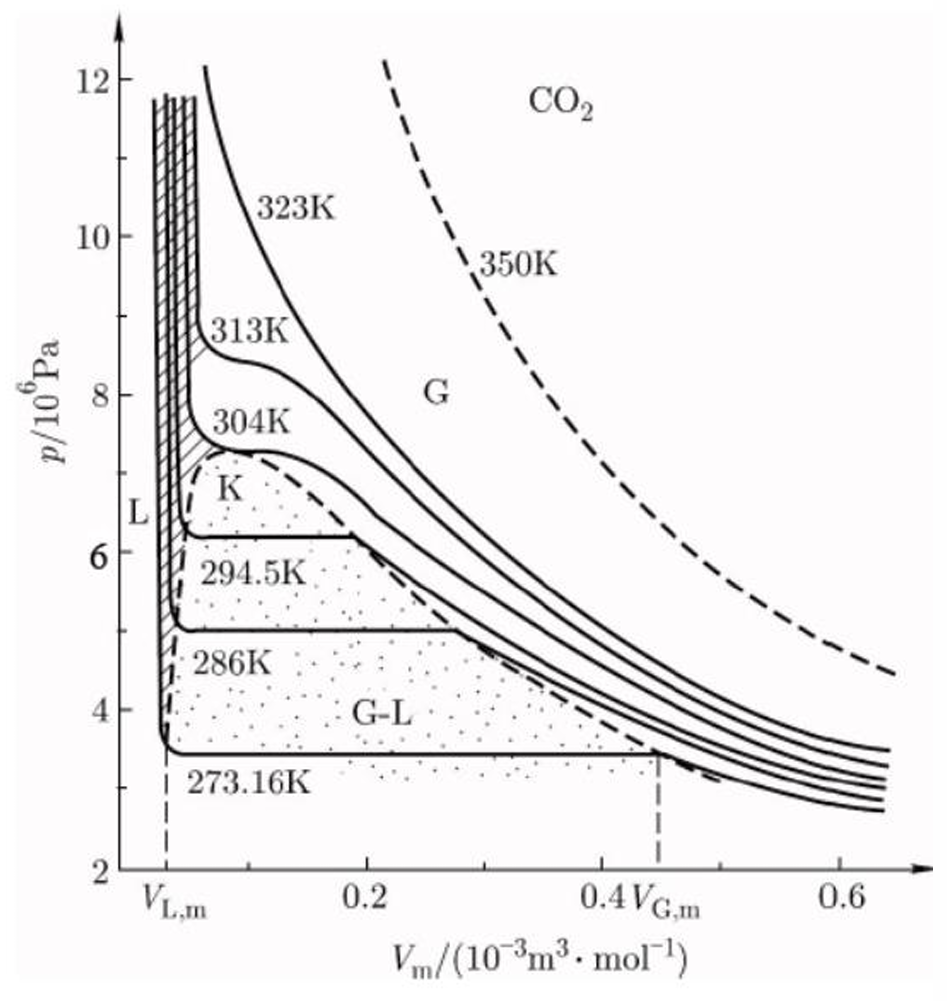
\includegraphics[width=0.5\textwidth]{andrews_isotherms.png}
  \caption{安德鲁斯实验：$\mathrm{CO_2}$ 的 $p$-$V$ 等温线}
  \label{fig:andrews_isotherms}
\end{figure}

\subsubsection{范德瓦尔斯等温线}

范德瓦尔斯方程：
\[
\left(p+\frac{a}{V_m^2}\right)(V_m-b)=RT
\]

可整理为 $V_m$ 的三次方程：
\[
V_m^3-\left(b+\frac{RT}{p}\right)V_m^2+\frac{a}{p}V_m-\frac{ab}{p}=0
\]

给定 $p,T$ 时，$V_m$ 的解有四种情况：

\begin{enumerate}[leftmargin=2em]
  \item[(I)] \textbf{三个不等实根}——对应相平衡（液气共存）；
  \item[(II)] \textbf{三个实根，两个相等}——对应单相-双相转变点；
  \item[(III)] \textbf{三个相等实根}——对应临界点 $K$；
  \item[(IV)] \textbf{一个实根、两个虚根}——对应单相（液相或气相）。
\end{enumerate}

\paragraph{Maxwell 等面积法则}
范德瓦尔斯等温线（如曲线 $ABCDE$）在相平衡区出现非物理的弯曲段。实际相平衡由水平等压线 $ACE$ 描述，其高度 $p^*$ 由\textbf{Maxwell 等面积法则}确定：

\[
\boxed{F_A^{\mathrm{mol}}-F_E^{\mathrm{mol}}
=\int_{ABCDE}p\,\mathrm{d}V^{\mathrm{mol}}
=p^*(V_G^{\mathrm{mol}}-V_L^{\mathrm{mol}})}
\]

即曲边形 $ABCA$ 的面积与曲边形 $CDEC$ 的面积相等。

相平衡条件为两相化学势相等：
\[
\boxed{\mu_A=\mu_E}
\]

% [插图：范德瓦尔斯等温线与 Maxwell 等面积法则示意图]
\begin{figure}[htbp]
  \centering
  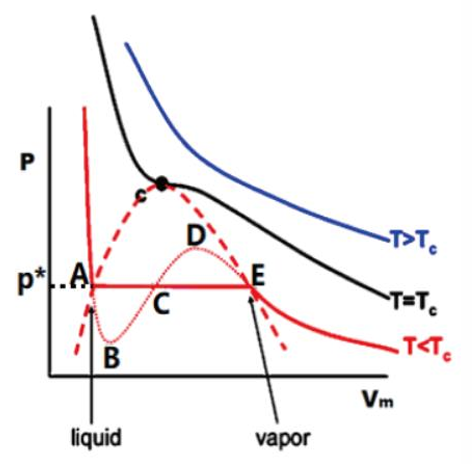
\includegraphics[width=0.4\textwidth]{van_der_waals_maxwell.png}
  \caption{范德瓦尔斯等温线与 Maxwell 等面积法则}
  \label{fig:van_der_waals_maxwell}
\end{figure}


% ============================================================
\subsection{相平衡时两相的物质的量之间的关系}
% ============================================================

以液气相变为例，设液相和气相的摩尔体积分别为 $V_L^{\mathrm{mol}},V_G^{\mathrm{mol}}$；系统总摩尔体积为 $\bar{V}$。两相的摩尔分数分别为：
\[
x_L=\frac{V_L}{V},\qquad x_G=\frac{V_G}{V}
\]

由总体积守恒：
\[
x_G V_G^{\mathrm{mol}}+x_L V_L^{\mathrm{mol}}=\bar{V},\qquad x_G+x_L=1
\]

解得：
\[
\boxed{x_L=\frac{V_G^{\mathrm{mol}}-\bar{V}}{V_G^{\mathrm{mol}}-V_L^{\mathrm{mol}}}},
\qquad
\boxed{x_G=\frac{\bar{V}-V_L^{\mathrm{mol}}}{V_G^{\mathrm{mol}}-V_L^{\mathrm{mol}}}}
\]

或写成对称形式：
\[
\boxed{x_G\bigl(V_G^{\mathrm{mol}}-\bar{V}\bigr)
=x_L\bigl(\bar{V}-V_L^{\mathrm{mol}}\bigr)}
\]

\textbf{结论}：一级相变平衡时，两相物质的摩尔百分比满足\textbf{杠杆原理}。

% [插图：杠杆原理示意图]
\begin{figure}[htbp]
  \centering
  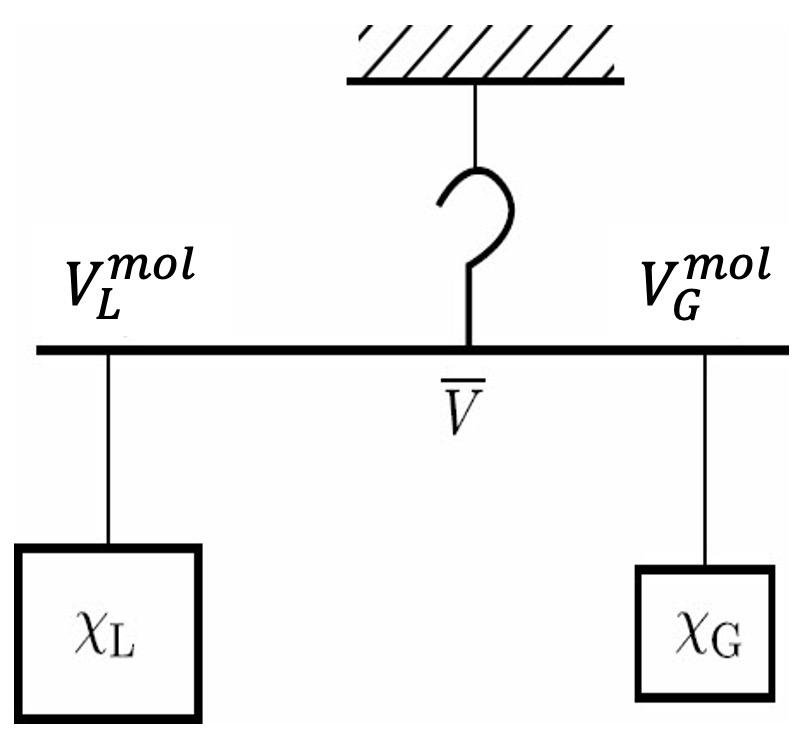
\includegraphics[width=0.4\textwidth]{lever_rule.png}
  \caption{相平衡时两相物质的量满足的杠杆原理}
  \label{fig:lever_rule}
\end{figure}


% ============================================================
\subsection{失稳分解与成核长大}
% ============================================================

\subsubsection{相分离判据与 \texorpdfstring{$p$-$V$}{p-V} 图分区}

相分离（失稳分解）的判据为系统自由能的二阶导数小于零：
\[
F_2<F_1\quad\text{即}\quad\frac{\mathrm{d}^2F_1}{\mathrm{d}V^2}<0
\]

由热力学基本方程 $\mathrm{d}F=-S\,\mathrm{d}T-p\,\mathrm{d}V$，得：
\[
\left(\frac{\partial F}{\partial V}\right)_T=-p,\qquad
\left(\frac{\partial^2 F}{\partial V^2}\right)_T
=-\left(\frac{\partial p}{\partial V}\right)_T
\]

因此，自由能曲线上关于 $\left(\dfrac{\partial^2 F}{\partial V^2}\right)_T$ 取特殊值的分区，可以在 $p$-$V$ 图上按 $-\left(\dfrac{\partial p}{\partial V}\right)_T$ 取相应特殊值而分区：

\begin{itemize}[leftmargin=2em]
  \item \textbf{稳定区}：$\left(\dfrac{\partial p}{\partial V}\right)_T<<0$（正常压缩）；
  \item \textbf{失稳分解区（Spinodal）}：$\left(\dfrac{\partial p}{\partial V}\right)_T>0$（非稳态，自动分相）；
  \item \textbf{成核长大区（Metastable）}：介于平衡曲线与失稳曲线之间，需克服势垒才能成核。
\end{itemize}

\subsubsection{弯曲液面的饱和蒸气压（开尔文公式）}

考虑弯曲液面的气液相平衡，设液面曲率半径为 $R$，表面张力系数为 $\alpha$。由相平衡条件及拉普拉斯公式，可得：

\[
(p'-p)+\frac{2\alpha}{R}\frac{V_l^{\mathrm{mol}}}{V_g^{\mathrm{mol}}-V_l^{\mathrm{mol}}}
=\frac{S_g^{\mathrm{mol}}-S_l^{\mathrm{mol}}}{V_g^{\mathrm{mol}}-V_l^{\mathrm{mol}}}\Delta T
\]

设 $\mu$ 为摩尔质量，$V_l^{\mathrm{mol}}=\mu/\rho_l$，$V_g^{\mathrm{mol}}=\mu/\rho_g$，且 $V_g\gg V_l$，则：

\[
\boxed{(p'-p)+\frac{2\alpha}{R}\frac{\rho_g}{\rho_l-\rho_g}
=\frac{\Lambda}{TV_g^{\mathrm{mol}}}\Delta T}
\]

\paragraph{讨论（$\Delta T=0$ 时）}
\begin{itemize}[leftmargin=2em]
  \item $R>0$（凹液面）：$p'<p$，\textbf{凹面液体的饱和蒸气压小于平面液体饱和蒸气压}；
  \item $R<<0$（凸液面）：$p'>p$，\textbf{凸面液体的饱和蒸气压大于平面液体饱和蒸气压}。
\end{itemize}

% [插图：弯曲液面气液平衡示意图]
\begin{figure}[htbp]
  \centering
  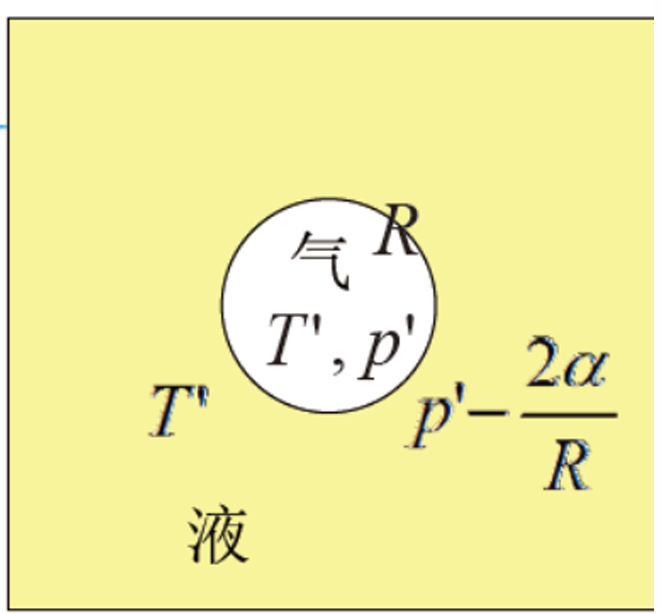
\includegraphics[width=0.35\textwidth]{curved_surface_vapor.png}
  \caption{弯曲液面的气液相平衡}
  \label{fig:curved_surface_vapor}
\end{figure}

\subsubsection{发生气液相变的临界半径}

令 $\Delta T=0$，由上述方程可得\textbf{临界半径}（中肯半径）：

\[
\boxed{R_c=-\frac{2\alpha\rho_g}{(p'-p)(\rho_l-\rho_g)}}
\]

\textbf{物理意义}：只有当生成核（气泡或液滴）的半径大于临界核的大小时，才能实现两相分离；否则核将自发消失。

\textbf{应用}：人工降雨（提供凝结核）、威尔逊云室等。


% ============================================================
\subsection{习题解答}
% ============================================================

\subsubsection{题 7.4（冰水相平衡曲线斜率）}

\textbf{题目}：在 $p_0=101325\ \mathrm{Pa}$ 下，冰的熔点为 $273.15\ \mathrm{K}$，熔解热 $l=3.35\times 10^5\ \mathrm{J/kg}$，冰的比体积 $v_\alpha=1.0907\times 10^{-3}\ \mathrm{m^3/kg}$，水的比体积 $v_\beta=1.00013\times 10^{-3}\ \mathrm{m^3/kg}$。求冰水两相平衡曲线的斜率 $\mathrm{d}p/\mathrm{d}T$。

\textbf{解}：冰水相变为一级相变，由克拉珀龙方程：
\[
\frac{\mathrm{d}p}{\mathrm{d}T}
=\frac{L_m}{T(V_{\beta,m}-V_{\alpha,m})}
=\frac{l_{\mathrm{sol}}}{T(v_\beta-v_\alpha)}
\]

代入数据：
\[
\frac{\mathrm{d}p}{\mathrm{d}T}
=\frac{3.35\times 10^5}{273.15\times(1.00013-1.0907)\times 10^{-3}}
\approx -1.354\times 10^7\ \mathrm{Pa/K}
\]

\[
\boxed{\frac{\mathrm{d}p}{\mathrm{d}T}\approx -1.35\times 10^7\ \mathrm{Pa/K}}
\]
（负号表明：对水而言，压强升高，熔点降低。）

\subsubsection{题 7.6（氨的熔点随压强变化）}

\textbf{题目}：在 $1\ \mathrm{atm}$ 下，固态氨于 $83\ \mathrm{K}$ 熔解，摩尔熔解热 $L_m=1176\ \mathrm{J/mol}$，摩尔体积增加 $\Delta V_{1,m}=3.5\times 10^{-6}\ \mathrm{m^3}$。有外力施加时，潜热保持不变，但体积变化与 $T^{3/2}$ 成反比。问：若要使熔点提高一倍，需施加多大压力？

\textbf{解}：由克拉珀龙方程：
\[
\frac{\mathrm{d}T}{\mathrm{d}p}
=\frac{T(V_{\beta,m}-V_{\alpha,m})}{L_m}
\]

依题意：
\[
L_m=\text{常量},\qquad
V_{\beta,m}-V_{\alpha,m}=KT^{-3/2}
\]

由参考态 $T_1=83\ \mathrm{K}$，$\Delta V_{1,m}=3.5\times 10^{-6}\ \mathrm{m^3}$，得：
\[
T^{3/2}(V_{\beta,m}-V_{\alpha,m})=T_1^{3/2}\Delta V_{1,m}
\]

即：
\[
T(V_{\beta,m}-V_{\alpha,m})=T_1^{3/2}\Delta V_{1,m}\,T^{-1/2}
\]

代入克拉珀龙方程并积分：
\[
\Delta p=\frac{L_m}{T_1^{3/2}\Delta V_{1,m}}
\cdot\frac{2}{3}\bigl(T_2^{3/2}-T_1^{3/2}\bigr)
=\frac{2L_m}{3\Delta V_{1,m}}
\left[\left(\frac{T_2}{T_1}\right)^{3/2}-1\right]
\]

代入 $T_2/T_1=2$：
\[
\Delta p=\frac{2\times 1176}{3\times 3.5\times 10^{-6}}\times(2^{3/2}-1)
\approx 4.1\times 10^8\ \mathrm{Pa}
\]

\[
\boxed{\Delta p\approx 4.1\times 10^8\ \mathrm{Pa}}
\]

\subsubsection{题 7.8（由沸点变化估算摩尔汽化热）}

\textbf{题目}：某液体在某一压强下沸点为 $400\ \mathrm{K}$，且沸点每升高 $1\ \mathrm{K}$，平衡压强升高 $5\%$。试估计该液体的摩尔汽化热。

\textbf{解}：液气相变中，$V_{G,m}\gg V_{L,m}$，且蒸气近似为理想气体 $V_{G,m}=RT/p$。由克拉珀龙方程：

\[
\frac{\mathrm{d}p}{\mathrm{d}T}
=\frac{L_m}{T(V_{G,m}-V_{L,m})}
\approx\frac{L_m}{TV_{G,m}}
=\frac{L_m p}{RT^2}
\]

分离变量：
\[
\frac{\mathrm{d}p}{p}=\frac{L_m}{R}\frac{\mathrm{d}T}{T^2}
\]

积分得：
\[
\ln\frac{p_f}{p_i}=\frac{L_m}{R}\left(\frac{1}{T_i}-\frac{1}{T_f}\right)
\]

即：
\[
L_m=\frac{RT_i T_f\ln(p_f/p_i)}{T_f-T_i}
\]

代入 $T_i=400\ \mathrm{K}$，$T_f=401\ \mathrm{K}$，$p_f=1.05p_i$：
\[
L_m=\frac{8.31\times 400\times 401\times\ln 1.05}{401-400}
\approx 6.50\times 10^4\ \mathrm{J/mol}
\]

\[
\boxed{L_m\approx 6.50\times 10^4\ \mathrm{J/mol}}
\]

\subsubsection{题 7.13（固体熔解的内能与熵增量）}

\textbf{题目}：质量为 $M$ 的固体，密度 $\rho_1$，在温度 $T$、压强 $p_1$ 下熔解成密度为 $\rho_2$ 的液体，熔解热为 $l$。求：(1) 内能增量；(2) 熵增量。

\textbf{解}：

(1) 由热力学第一定律：
\[
\Delta U=Q_{\text{吸}}-p_1(V_L-V_S)
\]

其中 $Q_{\text{吸}}=Ml$，且
\[
V_L-V_S=\frac{M}{\rho_2}-\frac{M}{\rho_1}
=M\left(\frac{1}{\rho_2}-\frac{1}{\rho_1}\right)
\]

故
\[
\boxed{\Delta U=M\left[l-p_1\left(\frac{1}{\rho_2}-\frac{1}{\rho_1}\right)\right]}
\]

(2) 固液相变为等温过程，熵增量：
\[
\Delta S=\frac{Q_{\text{吸}}}{T}=\frac{Ml}{T}
\]

\[
\boxed{\Delta S=\frac{Ml}{T}}
\]

\subsubsection{题 7.15（范德瓦尔斯等温线极值点轨迹）}

\textbf{题目}：证明将 $p$-$V$ 图上不同温度下范德瓦尔斯模型等温线的极小值点和极大值点连起来的曲线方程为 $pV_m^3=a(V_m-2b)$。

\textbf{证明}：$1\ \mathrm{mol}$ 范德瓦尔斯气体状态方程：
\[
\left(p+\frac{a}{V_m^2}\right)(V_m-b)=RT
\]

取全微分：
\[
R\,\mathrm{d}T
=p\,\mathrm{d}V_m-\frac{a}{V_m^2}\,\mathrm{d}V_m
+\frac{2ab}{V_m^3}\,\mathrm{d}V_m+(V_m-b)\,\mathrm{d}p
\]

等温过程 $\mathrm{d}T=0$，故：
\[
\frac{\mathrm{d}p}{\mathrm{d}V_m}
=-\frac{p-\dfrac{a}{V_m^2}+\dfrac{2ab}{V_m^3}}{V_m-b}
\]

极值点处 $\dfrac{\mathrm{d}p}{\mathrm{d}V_m}=0$，即：
\[
p-\frac{a}{V_m^2}+\frac{2ab}{V_m^3}=0
\quad\Longrightarrow\quad
p=\frac{a}{V_m^2}-\frac{2ab}{V_m^3}
\]

两边同乘 $V_m^3$：
\[
\boxed{pV_m^3=aV_m-2ab=a(V_m-2b)}
\]

证毕。

\subsubsection{题 7.16（碳纳米管中水的凝结温度）}

\textbf{题目}：碳纳米管中水与管壁接触角为 $\theta$，管半径 $R_p$，水的表面张力系数 $\sigma$，平面水的凝结温度为 $T_{S,B}$，冰的熔解热 $l$，密度 $\rho$。

(1) 证明碳纳米管中水的凝结温度改变量为
\[
\Delta T_S=T_{S,P}-T_{S,B}=-\frac{2\sigma\cos\theta}{l\rho R_p}T_{S,B}
\]

(2) 实验数据如下表，总结 $\Delta T_S$ 与 $D_p$ 的关系。

\begin{center}
\begin{tabular}{c|ccccccc}
\hline
$D_p/\mathrm{nm}$ & 1.35 & 1.70 & 1.87 & 3.21 & 6.57 & 8.17 & 8.86 \\
\hline
$\Delta T_S/\mathrm{K}$ & $-21.0$ & $-15.0$ & $-14.2$ & $-10.5$ & $-7.5$ & $-6.5$ & $-4.5$ \\
\hline
\end{tabular}
\end{center}

(3) 讨论表面张力系数与管径的关系。

\textbf{解}：

(1) 平面液面时相平衡条件：$\mu_i(T,p)=\mu_w(T,p)$。

碳纳米管中，弯曲液面使液相压强改变。由拉普拉斯公式，液相压强为 $p'-\dfrac{2\sigma\cos\theta}{R_p}$。相平衡条件变为：
\[
\mu_i(T',p')=\mu_w\!\left(T',p'-\frac{2\sigma\cos\theta}{R_p}\right)
\]

利用 $\mathrm{d}\mu_m=\mathrm{d}G_m=V_m\,\mathrm{d}p-S_m\,\mathrm{d}T$，分别展开两边并相减，整理得：

\[
\Delta T_S
=\frac{V_{i,m}-V_{w,m}}{S_{i,m}-S_{w,m}}(p'-p)
+\frac{2\sigma\cos\theta}{R_p}\frac{V_{w,m}}{S_{i,m}-S_{w,m}}
\]

由 $p'-p=\dfrac{2\sigma\cos\theta}{R_p}$（拉普拉斯公式）及
\[
V_m=\frac{M}{\rho},\qquad
S_{i,m}-S_{w,m}=-\frac{L_m}{T}=-\frac{lM}{T_{S,B}}
\]

代入整理得：
\[
\boxed{\Delta T_S=-\frac{2\sigma\cos\theta}{l\rho_i R_p}T_{S,B}}
\]

(2) 将实验数据整理为 $\Delta T_S D_p$：

\begin{center}
\begin{tabular}{c|ccccccc}
\hline
$D_p/\mathrm{nm}$ & 1.35 & 1.70 & 1.87 & 3.21 & 6.57 & 8.17 & 8.86 \\
\hline
$\Delta T_S/\mathrm{K}$ & $-21.0$ & $-15.0$ & $-14.2$ & $-10.5$ & $-7.5$ & $-6.5$ & $-4.5$ \\
\hline
$\Delta T_S D_p/(\mathrm{nm\cdot K})$ & $-28.35$ & $-25.5$ & $-26.55$ & $-33.71$ & $-49.28$ & $-53.11$ & $-39.87$ \\
\hline
\end{tabular}
\end{center}

显然 $\Delta T_S D_p$ 不是常量，与简单理论（假设 $\sigma$ 为常量）不符。对实验数据进行拟合，假设：
\[
\Delta T_S=\frac{a}{D_p}\left(1+\frac{b}{D_p^2}\right)
\]

最小误差拟合得 $a=-33.38\ \mathrm{nm\cdot K}$，$b=-0.39\ \mathrm{nm^2}$。实验测得的关系为：
\[
\Delta T_S=-\frac{33.38}{D_p}\left(1-\frac{0.39}{D_p^2}\right)
\]

定性上与理论一致（$\Delta T_S\propto 1/D_p$），定量上有偏差。

(3) 比较实验与理论可知，碳纳米管中水的表面张力系数与管径的关系可表示为：
\[
\boxed{\sigma=\sigma_0\left(1-\frac{0.39}{D_p^2}\right)}
\]

\textbf{结论}：碳纳米管中水的表面张力系数随管内直径减小而减小；由于 $D_p^2$ 正比于管内弯曲水面的面积，说明纳米尺度下表面张力系数不再与面积无关，而是随面积减小而减小。

\newpage
% ============================================================
\section{第一章补充：平衡态与状态方程}
% ============================================================

\subsection{状态参量与平衡态}

\paragraph{热力学系统}
由大量微观粒子组成的宏观物体，可分为孤立系、封闭系与开放系。

\paragraph{状态参量}
描述系统宏观状态的物理量，如压强 $p$、体积 $V$、温度 $T$ 等。

\paragraph{平衡态}
在不受外界影响的条件下，系统的宏观性质不随时间变化的状态。

\subsection{温度与温标}

\paragraph{热力学第零定律}
若系统 $A$ 与系统 $B$ 分别与系统 $C$ 达到热平衡，则 $A$ 与 $B$ 彼此也处于热平衡。

\paragraph{理想气体温标}
由查理定律（Charles's law）与盖–吕萨克定律（Gay-Lussac's law），当 $p\to 0$ 时实际气体趋于理想气体：
\[
T_V(p)=273.15\lim_{p_0\to 0}\left(\frac{p}{p_0}\right),\qquad
T_p(V)=273.15\lim_{p_0\to 0}\left(\frac{V}{V_0}\right)
\]

理想气体温标与摄氏温标的关系：
\[
\boxed{T/\mathrm{K}=273.15+t/^{\circ}\mathrm{C}}
\]

\subsection{摩尔与阿伏伽德罗常量}

\paragraph{摩尔（mole）}
$1\ \mathrm{mol}$ 物质所包含的粒子数与 $12\ \mathrm{g}\ ^{12}\mathrm{C}$ 中的原子数精确相等。

\paragraph{阿伏伽德罗常量}
\[
N_A=6.02214076\times 10^{23}\ \mathrm{mol^{-1}}
\]

\paragraph{摩尔质量}
$1\ \mathrm{mol}$ 物质的质量。单个分子质量 $m=\dfrac{M_{\mathrm{mol}}}{N_A}$。

\paragraph{气体常量}
\[
R=k_B N_A=8.314462618\ \mathrm{J/(K\cdot mol)}
\]

\subsection{状态方程}

\paragraph{理想气体状态方程}
\[
\boxed{pV=\nu RT}
\]

\paragraph{范德瓦尔斯方程}
对 $1\ \mathrm{mol}$ 气体：
\[
\boxed{\left(p+\frac{a}{V_m^2}\right)(V_m-b)=RT}
\]
对 $\nu\ \mathrm{mol}$ 气体：
\[
\left(p+\frac{\nu^2 a}{V^2}\right)(V-\nu b)=\nu RT
\]

\paragraph{混合理想气体}
\[
\nu=\nu_1+\nu_2+\cdots+\nu_n
\]
道尔顿分压定律：
\[
\boxed{p=\sum_i p_i}
\]

\subsection{温度的统计意义与微观解释}

\paragraph{理想气体压强公式}
\[
\boxed{p=\frac{2}{3}n\overline{E_k}}
\]

\paragraph{温度与平均平动动能}
\[
\boxed{\overline{E_k}=\frac{3}{2}k_B T}
\]
理想气体的温度正比于分子无规则运动的平均平动动能。

\paragraph{玻尔兹曼常量}
\[
k_B=\frac{R}{N_A}=1.380649\times 10^{-23}\ \mathrm{J/K}\approx 8.617\times 10^{-5}\ \mathrm{eV/K}
\]


% ============================================================
\section{第二章补充：平衡态系统的统计规律}
% ============================================================

\subsection{麦克斯韦速率分布}

\paragraph{速率分布函数}
\[
f(v)=4\pi v^2\left(\frac{m}{2\pi k_B T}\right)^{3/2}\exp\!\left(-\frac{mv^2}{2k_B T}\right)
\]

\paragraph{三种特征速率}
\begin{center}
\begin{tabular}{c|c|c}
\hline
名称 & 公式 & 数值比 \\
\hline
最概然速率 & $\displaystyle v_p=\sqrt{\frac{2k_B T}{m}}=\sqrt{\frac{2RT}{M}}$ & $1$ \\
平均速率 & $\displaystyle \bar{v}=\sqrt{\frac{8k_B T}{\pi m}}=\sqrt{\frac{8RT}{\pi M}}$ & $\sqrt{\dfrac{4}{\pi}}\approx 1.128$ \\
方均根速率 & $\displaystyle v_{\mathrm{rms}}=\sqrt{\frac{3k_B T}{m}}=\sqrt{\frac{3RT}{M}}$ & $\sqrt{\dfrac{3}{2}}\approx 1.225$ \\
\hline
\end{tabular}
\end{center}

三者之比：
\[
\boxed{v_p:\bar{v}:v_{\mathrm{rms}}=\sqrt{2}:\sqrt{\frac{8}{\pi}}:\sqrt{3}\approx 1.414:1.596:1.732}
\]

\subsection{麦克斯韦速度分布}

\paragraph{速度分布函数}
\[
f(v_x,v_y,v_z)=\left(\frac{m}{2\pi k_B T}\right)^{3/2}
\exp\!\left[-\frac{m(v_x^2+v_y^2+v_z^2)}{2k_B T}\right]
\]

\paragraph{分量分布}
各速度分量独立服从高斯分布：
\[
f(v_x)=\left(\frac{m}{2\pi k_B T}\right)^{1/2}\exp\!\left(-\frac{mv_x^2}{2k_B T}\right)
\]

\paragraph{碰壁数（单位面积单位时间）}
\[
\boxed{\Gamma=\frac{1}{4}n\bar{v}}
\]

\subsection{玻尔兹曼分布}

\paragraph{按能量分布}
\[
\mathrm{d}N=n_0\left(\frac{m}{2\pi k_B T}\right)^{3/2}
\exp\!\left(-\frac{\varepsilon_p+\varepsilon_k}{k_B T}\right)
\mathrm{d}v_x\mathrm{d}v_y\mathrm{d}v_z\mathrm{d}x\mathrm{d}y\mathrm{d}z
\]

\paragraph{按高度分布（重力场中）}
\[
n=n_0\exp\!\left(-\frac{mgz}{k_B T}\right)
\quad\Longrightarrow\quad
p=p_0\exp\!\left(-\frac{Mgz}{RT}\right)
\]
由此可得等温大气压强公式：
\[
\boxed{z=\frac{RT}{Mg}\ln\frac{p_0}{p}}
\]

\subsection{能均分定理}

\paragraph{定理内容}
平衡态下，物质分子的每一个自由度都具有平均能量 $\dfrac{1}{2}k_B T$。

\paragraph{分子能量}
设分子有 $t$ 个平动、$r$ 个转动、$s$ 个振动自由度，则平均能量：
\[
\boxed{\bar{\varepsilon}=\frac{1}{2}(t+r+2s)k_B T}
\]
（每个振动自由度贡献 $2\times\frac{1}{2}k_B T$，含动能与势能）

\paragraph{理想气体内能与摩尔热容}
\begin{center}
\begin{tabular}{c|c|c|c}
\hline
分子类型 & 自由度 & 内能 $U_m$ & $C_{V,m}$ \\
\hline
单原子（刚性） & $t=3,r=0,s=0$ & $\dfrac{3}{2}RT$ & $\dfrac{3}{2}R$ \\
双原子（刚性） & $t=3,r=2,s=0$ & $\dfrac{5}{2}RT$ & $\dfrac{5}{2}R$ \\
双原子（非刚性） & $t=3,r=2,s=1$ & $\dfrac{7}{2}RT$ & $\dfrac{7}{2}R$ \\
多原子（刚性） & $t=3,r=3,s=0$ & $3RT$ & $3R$ \\
\hline
\end{tabular}
\end{center}


% ============================================================
\section{第三章补充：近平衡态中的输运过程}
% ============================================================

\subsection{平均碰撞频率与平均自由程}

\paragraph{平均碰撞频率}
以分子有效直径 $d$ 形成的碰撞截面 $\sigma=\pi d^2$，平均碰撞频率：
\[
\boxed{\bar{Z}=\sqrt{2}\sigma\bar{v}n=\sqrt{2}\pi d^2\bar{v}n}
\]

\paragraph{平均自由程}
\[
\boxed{\bar{\lambda}=\frac{\bar{v}}{\bar{Z}}=\frac{1}{\sqrt{2}\sigma n}
=\frac{k_B T}{\sqrt{2}\sigma p}}
\]

当压强足够小（真空）时，$\bar{\lambda}$ 可大于容器线度 $L$，此时 $\bar{\lambda}\approx L$。

% [插图：分子碰撞与有效直径示意图]
\begin{figure}[htbp]
  \centering
  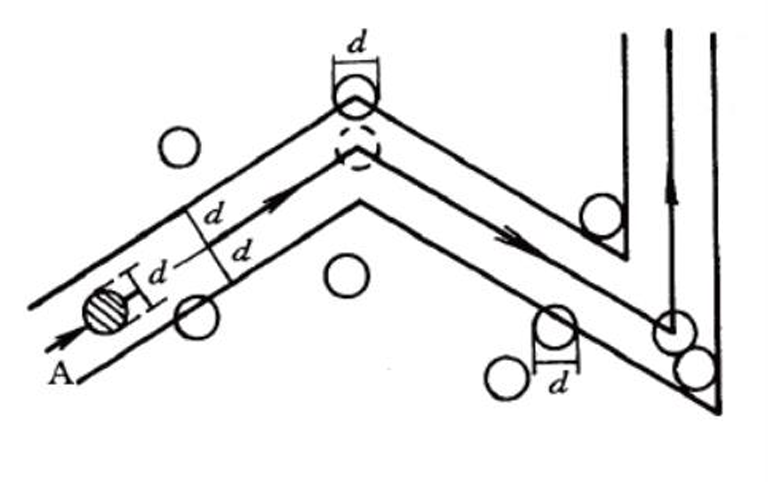
\includegraphics[width=0.5\textwidth]{collision_cross_section.png}
  \caption{分子碰撞截面与平均自由程示意图}
  \label{fig:collision}
\end{figure}

\subsection{输运过程的宏观规律}

\paragraph{黏滞现象（牛顿黏性定律）}
\[
\mathrm{d}K=-\eta\left(\frac{\mathrm{d}u}{\mathrm{d}z}\right)_{z_0}\mathrm{d}S\,\mathrm{d}t,
\qquad
F=\eta\left(\frac{\mathrm{d}u}{\mathrm{d}z}\right)_{z_0}\mathrm{d}S
\]

\paragraph{热传导（傅里叶定律）}
\[
\mathrm{d}Q=-\kappa\left(\frac{\mathrm{d}T}{\mathrm{d}z}\right)_{z_0}\mathrm{d}S\,\mathrm{d}t
\]

\paragraph{扩散（菲克定律）}
\[
\mathrm{d}m_g=-D\left(\frac{\mathrm{d}\rho}{\mathrm{d}z}\right)_{z_0}\mathrm{d}S\,\mathrm{d}t
\]

\subsection{输运系数的微观推导}

\paragraph{基本关系}
对理想气体，输运系数可近似表示为：
\[
\boxed{D\approx\frac{1}{3}\bar{v}\bar{\lambda}},\qquad
\boxed{\eta\approx\frac{1}{3}\rho\bar{v}\bar{\lambda}},\qquad
\boxed{\kappa\approx\frac{1}{3}\rho\bar{v}\bar{\lambda}c_V}
\]

或写成：
\[
\eta=\frac{\alpha_\eta}{\alpha_D}\rho D,\qquad
\kappa=\frac{\alpha_\kappa}{\alpha_\eta}c_V\eta
\]

其中 $\alpha_D,\alpha_\eta,\alpha_\kappa$ 为数量级为 $1$ 的系数。

\paragraph{单位}
\begin{itemize}[leftmargin=2em]
  \item 扩散系数 $D$：$\mathrm{m^2/s}$
  \item 黏度 $\eta$：$\mathrm{N\cdot s/m^2}$ 或 $\mathrm{Pa\cdot s}$
  \item 热导率 $\kappa$：$\mathrm{W/(m\cdot K)}$
\end{itemize}

\subsection{布朗运动}

\paragraph{爱因斯坦关系}
布朗粒子在流体中的扩散系数：
\[
\boxed{D=\frac{k_B T}{6\pi a\eta}}
\]
其中 $a$ 为粒子半径，$\eta$ 为流体黏度。

\paragraph{位移公式}
\[
\boxed{\overline{x^2}=2Dt}
\]

% ============================================================
\section{第四章补充：热力学第一定律的应用}
% ============================================================

\subsection{热容量}

\paragraph{定义}
在一定条件下，物体或系统温度升高（或降低）$1\ \mathrm{K}$时吸收（或放出）的热量。

\paragraph{等体过程}
\[
\Delta V=0\quad\Longrightarrow\quad (\Delta Q)_V=(\Delta U)_V
\]
等体热容：
\[
\boxed{C_V=\lim_{\Delta T\to 0}\frac{(\Delta Q)_V}{\Delta T}
=\left(\frac{\partial U}{\partial T}\right)_V}
\]

\paragraph{等压过程}
\[
(\Delta Q)_p=(\Delta U+p\Delta V)_p=[\Delta(U+pV)]_p
\]
定义\textbf{焓}（Enthalpy，状态函数）$H=U+pV$，则 $(\Delta Q)_p=(\Delta H)_p$。

等压热容：
\[
\boxed{C_p=\lim_{\Delta T\to 0}\frac{(\Delta Q)_p}{\Delta T}
=\left(\frac{\partial H}{\partial T}\right)_p}
\]

\paragraph{比热容与绝热指数}
\[
c_V=\frac{C_V}{m},\qquad c_p=\frac{C_p}{m},\qquad
\boxed{\gamma=\frac{C_p}{C_V}=\frac{C_p^{\mathrm{mol}}}{C_V^{\mathrm{mol}}}}
\]

\subsection{内能和焓}

\paragraph{定义}
\begin{itemize}[leftmargin=2em]
  \item 内能：$U=U_k+U_p=U(T,V)$，是态函数
  \item 焓：$H=U+pV=H(T,p)$，是态函数
\end{itemize}

\paragraph{计算}
\[
\mathrm{d}U=\left(\frac{\partial U}{\partial T}\right)_V\mathrm{d}T
+\left(\frac{\partial U}{\partial V}\right)_T\mathrm{d}V
=C_V\mathrm{d}T+f'(T,V)\mathrm{d}V
\]
\[
\mathrm{d}H=\left(\frac{\partial H}{\partial T}\right)_p\mathrm{d}T
+\left(\frac{\partial H}{\partial p}\right)_T\mathrm{d}p
=C_p\mathrm{d}T+g'(T,p)\mathrm{d}p
\]

积分形式：
\[
U(T,V)-U_0=\int_{T_0}^T C_V\mathrm{d}T+f(V),\qquad
H(T,p)-H_0=\int_{T_0}^T C_p\mathrm{d}T+g(p)
\]

\paragraph{实用说明}
\begin{itemize}[leftmargin=2em]
  \item 由于体膨胀系数 $\alpha\neq 0$，温度变化时体积也会变化，因此定体热容量实验上难以测定，而定压热容量测定相对容易。
  \item 地球表面物体一般处于确定大气压下，物态变化及化学反应多在定压下进行，因此\textbf{焓比内能有更重要的实用价值}。
\end{itemize}

\subsection{理想气体的内能、焓及热容量}

\paragraph{理想气体特性}
分子间相互作用可忽略，$U_p=\text{常量}$，故内能和热容都只是温度的函数：
\[
U=U(T)\quad\Longrightarrow\quad H=U(T)+\nu RT=H(T)
\]

\paragraph{迈耶公式}
\[
C_p=\left(\frac{\partial H}{\partial T}\right)_p=\left(\frac{\partial U}{\partial T}\right)_V+\nu R
=C_V+\nu R
\quad\Longrightarrow\quad
\boxed{C_p^{\mathrm{mol}}-C_V^{\mathrm{mol}}=R}
\]

\paragraph{绝热指数}
\[
\boxed{\gamma=\frac{C_p^{\mathrm{mol}}}{C_V^{\mathrm{mol}}}=1+\frac{R}{C_V^{\mathrm{mol}}}}
\quad\Longrightarrow\quad
C_V^{\mathrm{mol}}=\frac{R}{\gamma-1},\quad
C_p^{\mathrm{mol}}=\frac{\gamma R}{\gamma-1}
\]

\paragraph{典型数值}
\begin{center}
\begin{tabular}{c|c|c|c}
\hline
分子类型 & $C_V^{\mathrm{mol}}$ & $C_p^{\mathrm{mol}}$ & $\gamma$ \\
\hline
单原子 & $\dfrac{3}{2}R$ & $\dfrac{5}{2}R$ & $\dfrac{5}{3}\approx 1.67$ \\
刚性双原子 & $\dfrac{5}{2}R$ & $\dfrac{7}{2}R$ & $\dfrac{7}{5}=1.40$ \\
\hline
\end{tabular}
\end{center}

\subsection{焦耳--汤姆孙实验}

\paragraph{1. 焦耳定律}
气体进行\textbf{绝热自由膨胀}（$Q=0,W=0$），过程前后内能相同。虽然体积变化，但温度不变。
\[
\boxed{\text{理想气体的内能只是温度的函数，与体积无关}}
\]

\paragraph{2. 焦耳--汤姆孙实验（节流过程）}
气体经过绝热节流过程后\textbf{焓不变}：
\[
U_1+p_1V_1=U_2+p_2V_2=\text{恒量}
\quad\Longrightarrow\quad
H_1=H_2
\]

\paragraph{3. 焦汤系数}
等焓情况下温度随压强的变化率：
\[
\boxed{\mu=\left(\frac{\partial T}{\partial p}\right)_H}
\]
\begin{itemize}[leftmargin=2em]
  \item $\mu>0$：正效应（节流后降温）
  \item $\mu<<0$：负效应（节流后升温）
\end{itemize}

\paragraph{4. 理想气体}
\[
pV=\nu RT,\quad U=U(T),\quad C_V=\frac{\mathrm{d}U}{\mathrm{d}T}
\]
\[
U=U_0+\nu\int_{T_0}^T C_{V,m}\mathrm{d}T,\qquad
H=H_0+\nu\int_{T_0}^T C_{p,m}\mathrm{d}T
\]
\[
C_{p,m}=C_{V,m}+R
\]

\subsection{范德瓦尔斯气体的焦--汤效应}

\paragraph{节流过程}
对于等焓过程：$\mathrm{d}H=0$，即
\[
\mathrm{d}H=\left(\frac{\partial H}{\partial T}\right)_p\mathrm{d}T
+\left(\frac{\partial H}{\partial p}\right)_T\mathrm{d}p=0
\]

\paragraph{焦汤系数推导}
\[
\mu=\left(\frac{\partial T}{\partial p}\right)_H
=-\frac{(\partial H/\partial p)_T}{(\partial H/\partial T)_p}
=\frac{-1}{C_p}\left(\frac{\partial H}{\partial p}\right)_T
\]
利用链式法则：
\[
\mu=\frac{-1}{C_p}\left(\frac{\partial H}{\partial V_m}\right)_T
\left(\frac{\partial V_m}{\partial p}\right)_T
\]

\paragraph{范德瓦尔斯气体状态方程}
\[
\left(p+\frac{a}{V_m^2}\right)(V_m-b)=RT
\quad\Longrightarrow\quad
p=\frac{RT}{V_m-b}-\frac{a}{V_m^2}
\]

\paragraph{摩尔内能与摩尔焓}
\[
U^{\mathrm{mol}}(T,V_m)=C_V^{\mathrm{mol}}T-\frac{a}{V_m}+U_0
\quad\text{（动能项+势能项+参考点）}
\]
\[
H^{\mathrm{mol}}(T,V_m)=U^{\mathrm{mol}}+pV_m
=C_V^{\mathrm{mol}}T+\frac{RTV_m}{V_m-b}-\frac{2a}{V_m}+H_0
\]

\paragraph{关键偏导数}
\[
\left(\frac{\partial H}{\partial V_m}\right)_T
=\frac{2a(V_m-b)^2-RTbV_m^2}{V_m^2(V_m-b)^2}
\]
\[
\left(\frac{\partial p}{\partial V_m}\right)_T
=\frac{-RT}{(V_m-b)^2}+\frac{2a}{V_m^3}
=\frac{2a(V_m-b)^2-RTV_m^3}{V_m^3(V_m-b)^2}
\]
\[
\left(\frac{\partial V_m}{\partial p}\right)_T
=\frac{V_m^3(V_m-b)^2}{2a(V_m-b)^2-RTV_m^3}<0
\]

\paragraph{焦汤系数表达式}
\[
\boxed{\mu=\frac{1}{C_p}\cdot
\frac{2aV_m(V_m-b)^2-RTbV_m^3}{RTV_m^3-2a(V_m-b)^2}}
\]

\paragraph{物理意义}
$\mu$ 的符号取决于\textbf{吸引势} $2aV_m(V_m-b)^2$ 与 \textbf{排斥势} $RTbV_m^3$ 的竞争：
\begin{itemize}[leftmargin=2em]
  \item $a$ 起主要作用（$r>r_0$）：JT为正效应
  \item $b$ 起主要作用（$r<<r_0$）：JT为负效应
\end{itemize}

\subsection{转换曲线}

\paragraph{$\mu=0$ 的条件}
\[
2aV_m(V_m-b)^2=RT_c bV_m^3
\]
解得转换曲线上的摩尔体积：
\[
V_m=\frac{b}{1-\sqrt{\dfrac{RT_c b}{2a}}}
\]

代入状态方程得转换曲线上压强与温度的关系 $p_c(T_c)$。

\paragraph{特征温度与压强}
\begin{itemize}[leftmargin=2em]
  \item 最高上转换温度：$T_c^u=\dfrac{2a}{Rb}$
  \item 最低下转换温度：$T_c^d=\dfrac{2a}{9Rb}$
  \item 最高压强：$p_{c0}=\dfrac{a}{3b^2}$（对应 $T_{c0}=\dfrac{8a}{9Rb}$）
\end{itemize}

\subsection{热力学第一定律对理想气体的应用}

\subsubsection{等体过程}

\paragraph{过程方程}
\[
V=\text{常量},\quad\text{或}\quad \frac{T}{p}=\text{常量}
\]

\paragraph{能量关系}
\[
\Delta V=0\quad\Longrightarrow\quad W=0\quad\Longrightarrow\quad \Delta U=Q
\]
\[
\mathrm{d}Q=\mathrm{d}U=\left(\frac{\partial U}{\partial T}\right)_V\mathrm{d}T=C_V\mathrm{d}T
\]
\[
\boxed{\Delta U=\int_{T_1}^{T_2}C_V\mathrm{d}T=C_V\Delta T}
\]

% [插图：等体过程 p-V 图]
\begin{figure}[htbp]
  \centering
  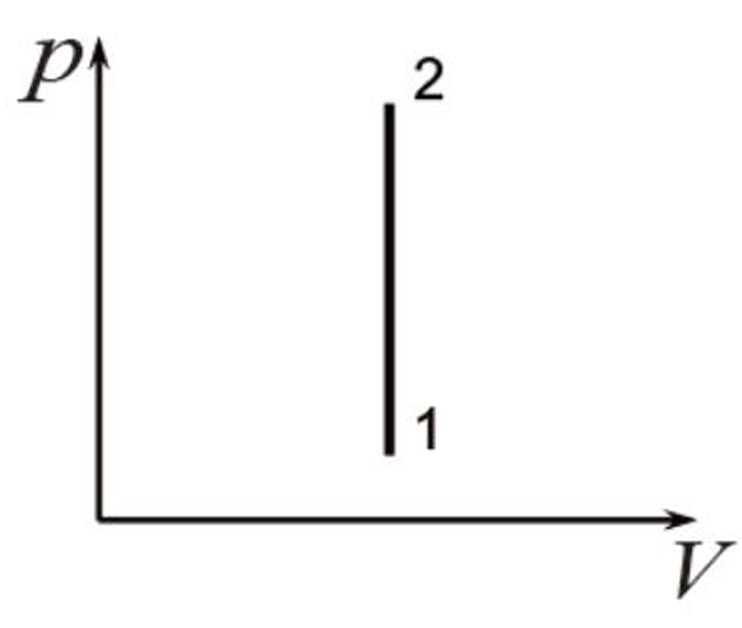
\includegraphics[width=0.3\textwidth]{isochoric_process.png}
  \caption{等体过程 $p$-$V$ 图}
  \label{fig:isochoric}
\end{figure}

\subsubsection{等压过程}

\paragraph{过程方程}
\[
p=\text{常量},\quad\text{或}\quad \frac{T}{V}=\text{常量}
\]

\paragraph{功}
\[
\mathrm{d}W=-p\,\mathrm{d}V,\qquad
W=-\int_{V_1}^{V_2}p\,\mathrm{d}V=-p(V_2-V_1)
\]

\paragraph{热量与焓变}
\[
\mathrm{d}Q_p=C_p\mathrm{d}T,\qquad
Q_p(1\to 2)=\int_{T_1}^{T_2}C_p\mathrm{d}T=C_p\Delta T
\]
\[
\Delta U=Q+W=C_p\Delta T-p(V_2-V_1)=(C_p-\nu R)\Delta T=C_V\Delta T
\]
\[
\boxed{Q=\Delta U-W=U_2-U_1+p(V_2-V_1)=H_2-H_1=\Delta H}
\]

\textbf{结论}：等压过程中系统焓的增量等于系统从外界吸收的热量。

% [插图：等压过程 p-V 图]
\begin{figure}[htbp]
  \centering
  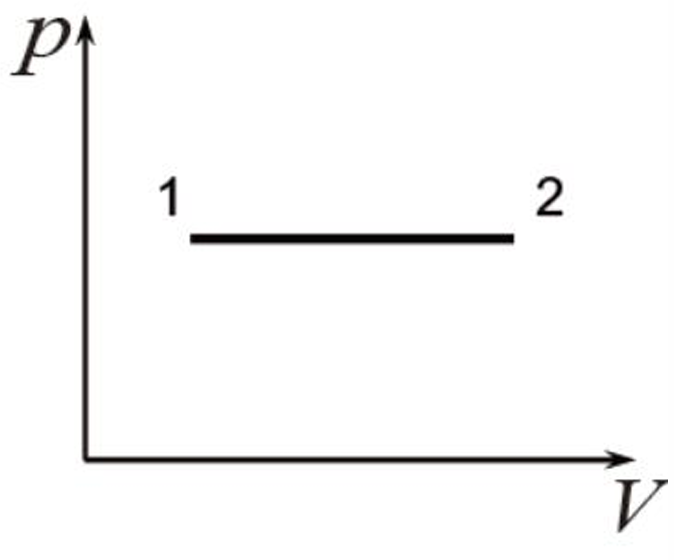
\includegraphics[width=0.3\textwidth]{isobaric_process.png}
  \caption{等压过程 $p$-$V$ 图}
  \label{fig:isobaric}
\end{figure}

\subsubsection{等温过程}

\paragraph{过程方程}
\[
T=\text{const}\quad\Longrightarrow\quad pV=\text{const}
\]

\paragraph{能量与功}
\[
U=U(T)\quad\Longrightarrow\quad \Delta U=0
\]
\[
Q=-W=\int_{V_1}^{V_2}p\,\mathrm{d}V
=\frac{m}{M}RT\int_{V_1}^{V_2}\frac{1}{V}\mathrm{d}V
\]
\[
\boxed{Q=\frac{m}{M}RT\ln\frac{V_2}{V_1}}
\]

\textbf{结论}：等温膨胀过程中，理想气体对外界做的功全部来源于从外界吸收的热量。

% [插图：等温过程 p-V 图]
\begin{figure}[htbp]
  \centering
  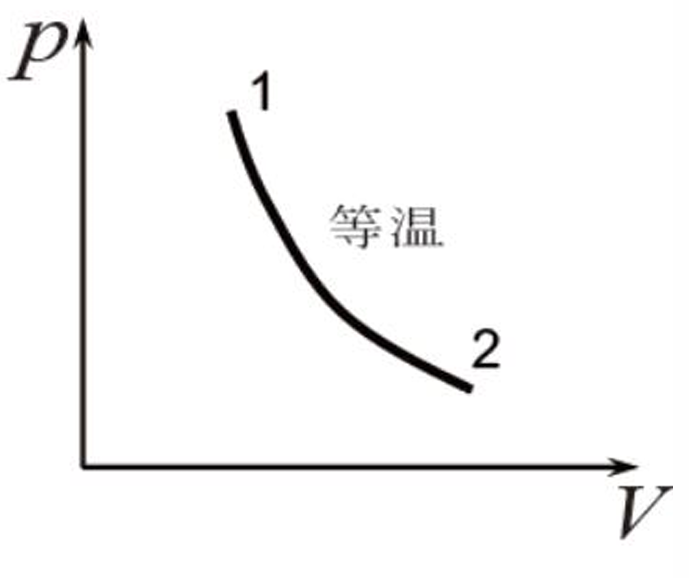
\includegraphics[width=0.3\textwidth]{isothermal_process.png}
  \caption{等温过程 $p$-$V$ 图}
  \label{fig:isothermal}
\end{figure}

\subsubsection{绝热过程}

\paragraph{基本关系}
\[
Q=0,\qquad \mathrm{d}U=C_V\mathrm{d}T=\mathrm{d}W=-p\,\mathrm{d}V
\]

\paragraph{泊松方程（绝热过程方程）}
由 $C_V\dfrac{\mathrm{d}T}{T}=-\dfrac{m}{M}R\dfrac{\mathrm{d}V}{V}=-(C_p-C_V)\dfrac{\mathrm{d}V}{V}$，积分得：
\[
\boxed{TV^{\gamma-1}=\text{const}},\qquad
\boxed{pV^{\gamma}=\text{const}},\qquad
\boxed{\frac{p^{\gamma-1}}{T^{\gamma}}=\text{const}}
\]

\paragraph{绝热线与等温线比较}
在 $p$-$V$ 图上，绝热线比等温线更陡（$\gamma>1$）。

\paragraph{绝热过程做功}
\[
W'=-W=\int_{V_1}^{V_2}p\,\mathrm{d}V
=p_1V_1^{\gamma}\int_{V_1}^{V_2}\frac{\mathrm{d}V}{V^{\gamma}}
=\frac{p_1V_1^{\gamma}}{\gamma-1}\left(V_1^{1-\gamma}-V_2^{1-\gamma}\right)
\]
\[
\boxed{W'=\frac{p_1V_1-p_2V_2}{\gamma-1}}
\]
利用 $pV=\nu RT$，也可写成：
\[
\boxed{W'=C_V(T_2-T_1)}
\]
即\textbf{绝热过程中外界对系统做的功等于系统内能的增量}。

% [插图：绝热与等温过程 p-V 图比较]
\begin{figure}[htbp]
  \centering
  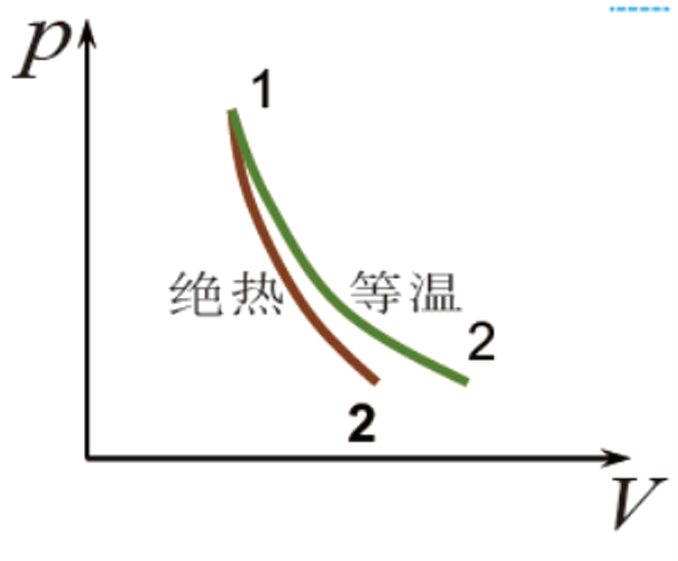
\includegraphics[width=0.3\textwidth]{adiabatic_vs_isothermal.png}
  \caption{绝热线与等温线比较（绝热线更陡）}
  \label{fig:adiabatic_isothermal}
\end{figure}

\subsubsection{干绝热递减率（DALR）}

\paragraph{温度随高度分布}
将大气视为理想气体，绝热上升过程中：
\[
\frac{\mathrm{d}T}{T}=\frac{\gamma-1}{\gamma}\frac{\mathrm{d}p}{p}
=-\frac{\gamma-1}{\gamma}\frac{Mg}{RT}\mathrm{d}z
\]
\[
\boxed{\frac{\mathrm{d}T}{\mathrm{d}z}=-\frac{\gamma-1}{\gamma}\frac{Mg}{R}
\approx -9.8\ \mathrm{K/km}\approx -10\ \mathrm{K/km}}
\]

\paragraph{温度与压强公式}
\[
T(z)=T_0\left[1-\left(\frac{Mg}{RT_0}\frac{\gamma-1}{\gamma}\right)z\right]
\quad\text{（线性关系）}
\]
\[
p(z)=p_0\left[1-\left(\frac{Mg}{RT_0}\frac{\gamma-1}{\gamma}\right)z\right]^{\frac{\gamma}{\gamma-1}}
\]

当 $\gamma\to 1$ 时，回到等温大气压强公式 $p=p_0\exp[-mgz/(k_BT)]$。

\subsubsection{多方过程}

\paragraph{过程方程}
前面几种准静态过程统一概括为：
\[
\boxed{pV^n=\text{const}}
\]
其中 $n$ 为\textbf{多方指数}。

\paragraph{特例}
\begin{center}
\begin{tabular}{c|c}
\hline
过程 & 多方指数 $n$ \\
\hline
等压 & $0$ \\
等温 & $1$ \\
绝热 & $\gamma$ \\
等体 & $\infty$ \\
\hline
\end{tabular}
\end{center}

\paragraph{等价形式}
\[
TV^{n-1}=\text{const},\qquad \frac{p^{n-1}}{T^n}=\text{const}
\]

\paragraph{做功、内能与传热}
\[
W=\frac{p_2V_2-p_1V_1}{n-1}=\frac{\nu R}{n-1}(T_2-T_1)
\]
\[
\Delta U=C_V(T_2-T_1)
\]
由第一定律：
\[
Q=C_n(T_2-T_1)=\Delta U-W
\]
\[
\boxed{C_n=C_V-\frac{\nu R}{n-1}}
\]

% [插图：多方过程在 p-V 图上的汇总]
\begin{figure}[htbp]
  \centering
  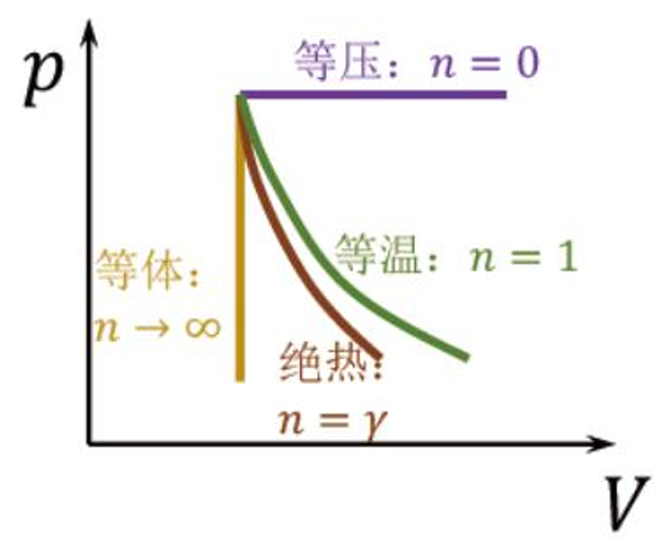
\includegraphics[width=0.4\textwidth]{polytropic_process_review.png}
  \caption{多方过程在 $p$-$V$ 图上的汇总}
  \label{fig:polytropic_review}
\end{figure}

\subsection{循环过程与卡诺循环}

\subsubsection{循环过程}

\paragraph{定义}
系统由某状态出发，经过任意一系列过程，最后回到原来状态。

\paragraph{$p$-$V$ 图表示}
准静态循环在 $p$-$V$ 图上为闭合曲线。
\begin{itemize}[leftmargin=2em]
  \item \textbf{符号约定}：顺时针为正，逆时针为负
  \item 循环性质：内能（状态函数）不变，$\Delta U=0$
\end{itemize}

\paragraph{正循环与逆循环}
\begin{itemize}[leftmargin=2em]
  \item \textbf{正循环}：$W'=Q>0$，系统对外界做功（热机）
  \item \textbf{逆循环}：$W'=Q<<0$，系统向外界放热（制冷机、热泵）
\end{itemize}

\paragraph{热机效率与制冷系数}
\[
\boxed{\eta=\frac{W'}{Q_1}=\frac{Q_1-Q_2'}{Q_1}}
\]
\[
\boxed{\varepsilon=\frac{Q_2}{W}=\frac{Q_2}{Q_1'-Q_2}}
\]

% [插图：循环过程 p-V 图]
\begin{figure}[htbp]
  \centering
  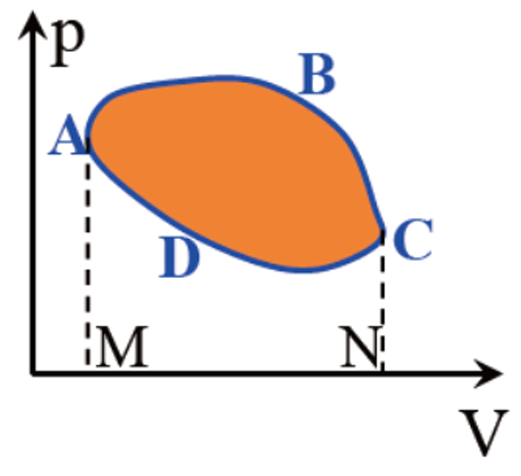
\includegraphics[width=0.4\textwidth]{cycle_process.png}
  \caption{循环过程 $p$-$V$ 图}
  \label{fig:cycle_process}
\end{figure}

\subsubsection{卡诺循环与卡诺热机}

\paragraph{组成}
由两个\textbf{等温过程}和两个\textbf{绝热过程}组成的循环。

\paragraph{各阶段特征}
\begin{itemize}[leftmargin=2em]
  \item $A\to B$：等温膨胀，吸热 $Q_1$，对外界做功
  \item $B\to C$：绝热膨胀，对外界做功
  \item $C\to D$：等温压缩，放热 $Q_2$，对系统做功
  \item $D\to A$：绝热压缩，对系统做功
\end{itemize}

\paragraph{卡诺热机效率}
利用绝热过程 $TV^{\gamma-1}=\text{常量}$，可得 $V_B/V_A=V_C/V_D$，于是：
\[
\eta=\frac{T_1\ln\dfrac{V_B}{V_A}-T_2\ln\dfrac{V_C}{V_D}}
{T_1\ln\dfrac{V_B}{V_A}}
\]
\[
\boxed{\eta=1-\frac{T_2}{T_1}}
\]

\paragraph{逆卡诺循环（制冷机）}
\[
\boxed{\varepsilon=\frac{Q_2}{W}=\frac{Q_2}{Q_1'-Q_2}
=\frac{T_2}{T_1-T_2}}
\]

% [插图：卡诺循环 p-V 图]
\begin{figure}[htbp]
  \centering
  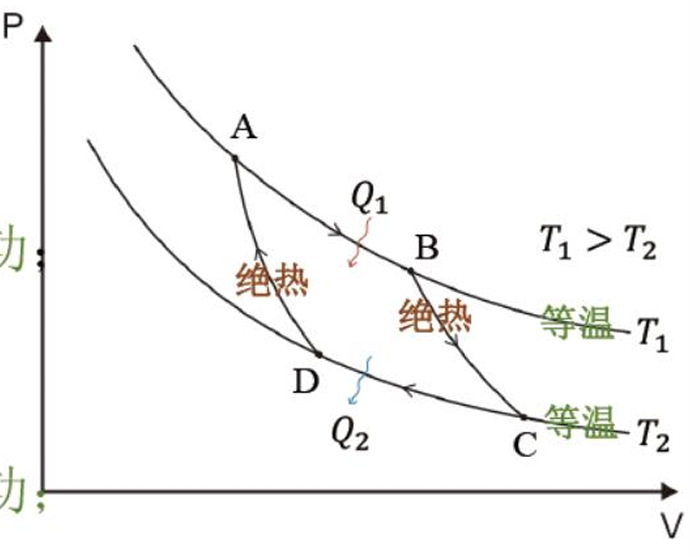
\includegraphics[width=0.45\textwidth]{carnot_cycle_review.png}
  \caption{卡诺循环 $p$-$V$ 图}
  \label{fig:carnot_cycle_review}
\end{figure}


% ============================================================
\section{第五章：热力学第二定律}
% ============================================================

\subsection{主要内容框架}

\begin{enumerate}[leftmargin=2em]
  \item 可逆过程与不可逆过程：概念；举例
  \item 热力学第二定律的两种语言表述：克劳修斯表述；开尔文表述；两种表述的等价性
  \item 热力学第二定律的数学表述：卡诺定理；热力学第二定律的数学表述；卡诺定理应用举例
  \item 熵与熵增加原理：熵的概念；熵变的计算；熵增加原理
  \item 熵及热力学第二定律的统计意义：玻尔兹曼熵；微观熵与宏观熵的关系
  \item 热力学第二定律的应用：热力学温标的建立
  \item 自由能、自由焓、化学势及热力学方程：亥姆霍兹自由能；吉布斯函数；化学势
  \item 热力学第三定律：熵的标准参考点；热力学第三定律
\end{enumerate}

\subsection{热力学第二定律的两种语言表述}

\paragraph{热机效率与制冷系数}
\[
\eta=\frac{Q_1-Q_2'}{Q_1},\qquad
\varepsilon=\frac{Q_2}{Q_1'-Q_2}
\]

\paragraph{克劳修斯表述（Clausius, 1850）}
\[
\boxed{\text{不可能把热量从低温物体传到高温物体而不产生任何其他影响。}}
\]

\paragraph{开尔文表述（Kelvin, 1851）}
\[
\boxed{\text{不可能从单一热源吸收热量使之完全转变为有用的功而不产生其他影响。}}
\]
或：\textbf{第二类永动机是不可能造成的。}

\paragraph{第二类永动机}
从单一热源吸热对外做功但不产生其它任何影响的机械。

% ============================================================
\subsection{两种表述的等价性}
% ============================================================

\paragraph{核心结论}
热力学第二定律的克劳修斯表述和开尔文表述\textbf{完全等价}：
\begin{itemize}[leftmargin=2em]
  \item 如果开尔文表述正确，则克劳修斯表述也正确
  \item 如果克劳修斯表述正确，则开尔文表述也正确
\end{itemize}

\paragraph{证明（反证法）}

\textit{由克劳修斯表述推导开尔文表述：}

假设克劳修斯表述不正确，即存在热量 $Q$ 自发从低温热源 $T_2$ 传到高温热源 $T_1$ 的过程 (a)。将其与一个卡诺热机 (b) 耦合：卡诺热机从 $T_1$ 吸热 $Q_1$，对外做功 $W'$，向 $T_2$ 放热 $Q$。

组合系统 (c) 的净效果：从 $T_1$ 吸收热量 $Q_1-Q$，全部转化为功 $W'$，而不产生其他影响。这正是第二类永动机，违反开尔文表述。

\begin{figure}[htbp]
\centering
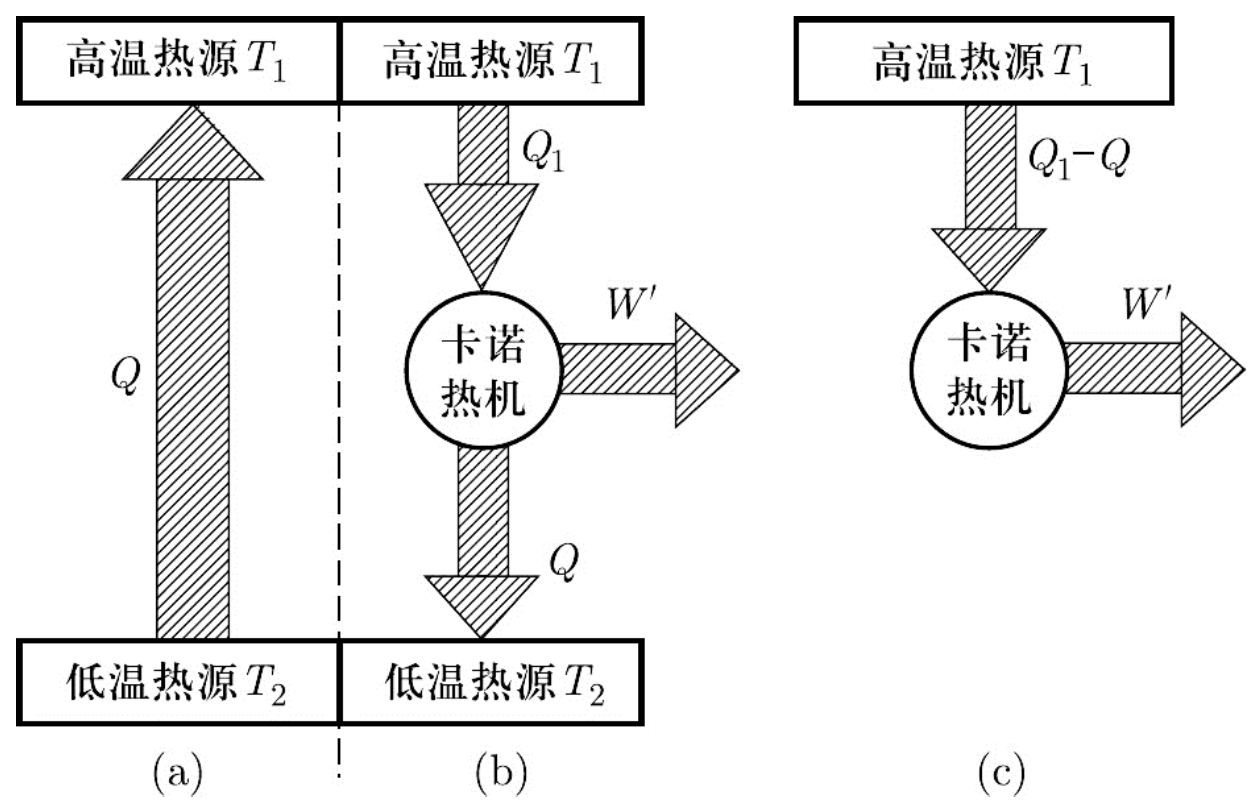
\includegraphics[width=0.6\textwidth]{equivalence_kelvin_clausius_1.png}
\caption{克劳修斯表述与开尔文表述等价性证明（一）}
\label{fig:equivalence1}
\end{figure}

\textit{由开尔文表述推导克劳修斯表述：}

同样用反证法。假设开尔文表述不对，即存在从单一热源 $T_1$ 吸热 $Q$ 全部变成功 $W'$ 的过程 (a)。用此功驱动制冷机 (b) 从 $T_2$ 吸热 $Q_2$，向 $T_1$ 放热 $Q_1'=Q+Q_2$。

组合系统 (c) 的净效果：热量 $Q_2$ 从低温 $T_2$ 传到高温 $T_1$，而不产生其他影响。违反克劳修斯表述。

\begin{figure}[htbp]
\centering
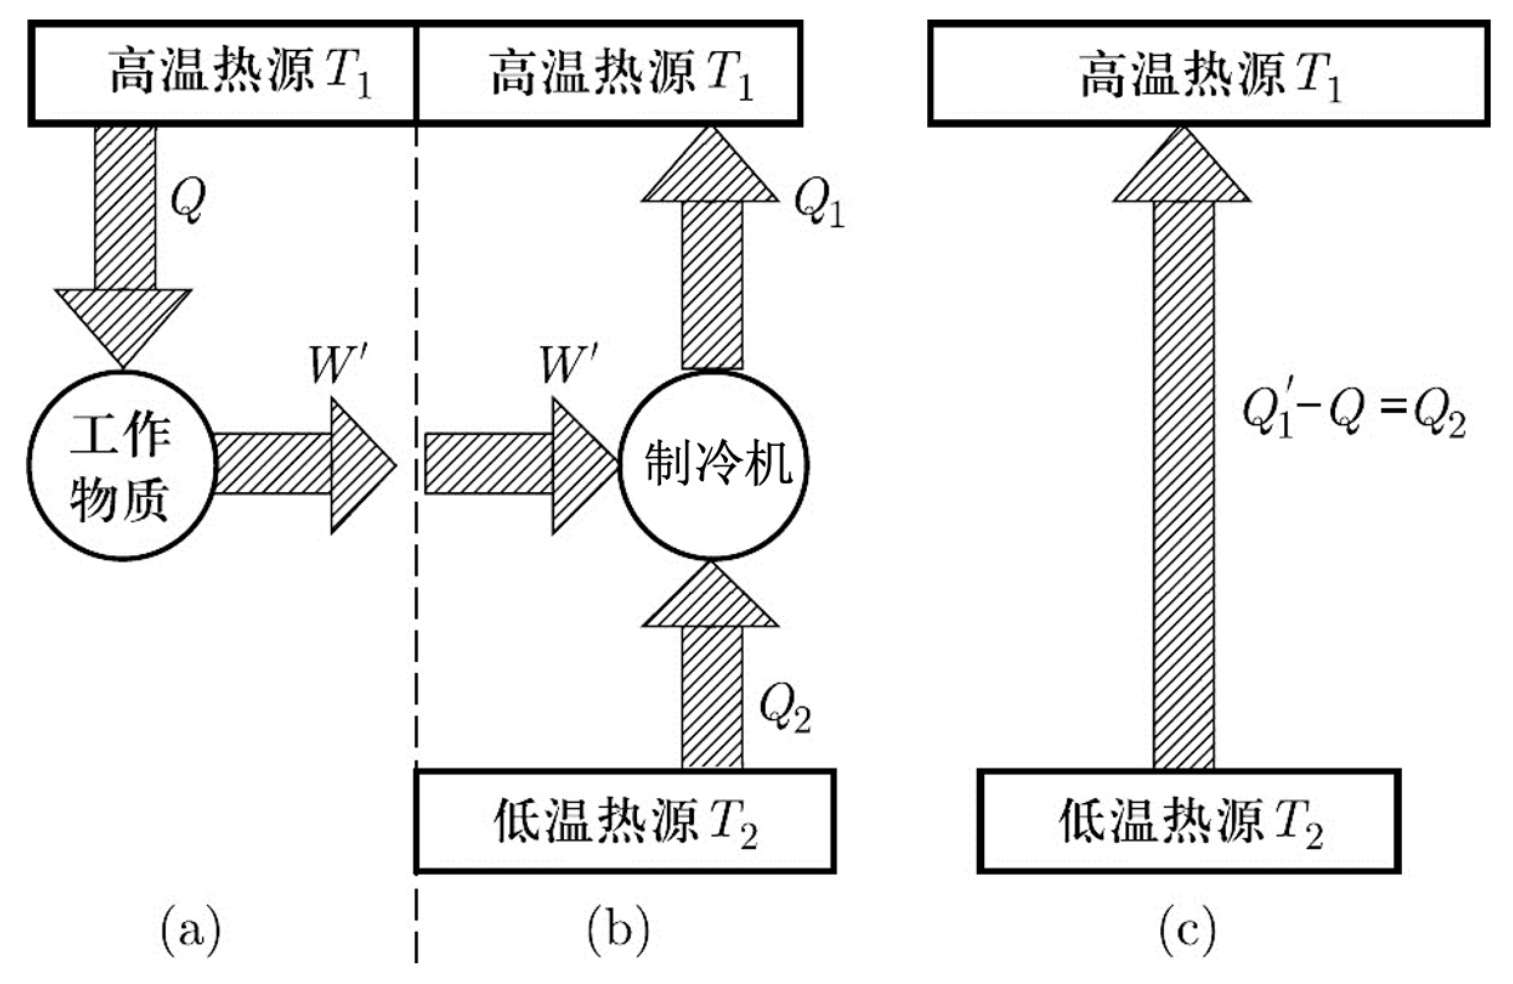
\includegraphics[width=0.6\textwidth]{equivalence_kelvin_clausius_2.png}
\caption{克劳修斯表述与开尔文表述等价性证明（二）}
\label{fig:equivalence2}
\end{figure}

% ============================================================
\subsection{卡诺定理}
% ============================================================

\paragraph{定理内容}
\begin{enumerate}[leftmargin=2em]
  \item 在相同的高温热源和相同的低温热源之间工作的一切\textbf{可逆热机}的效率都相等，与工作物质无关；
  \item 在相同的高温热源和相同的低温热源之间工作的一切\textbf{不可逆热机}的效率 $\eta'$ 都小于可逆热机的效率 $\eta$。
\end{enumerate}

\[
\boxed{\eta'=1-\frac{Q_2'}{Q_1}\le 1-\frac{T_2}{T_1}=\eta}
\]

\paragraph{对制冷机的推广}
\begin{enumerate}[leftmargin=2em]
  \item[(3)] 在相同的高温热源和相同的低温热源之间工作的一切\textbf{可逆制冷机}的效率（制冷系数）都相等，与工作物质无关；
  \item[(4)] 在相同的高温热源和相同的低温热源之间工作的一切\textbf{不可逆制冷机}的效率 $\varepsilon'$ 都小于可逆制冷机的效率 $\varepsilon$。
\end{enumerate}

\paragraph{卡诺定理应用：非理想气体内能方程}
考虑一个微小的卡诺正循环，利用循环效率与内能关系，可得\textbf{内能方程}：
\[
\boxed{\left(\frac{\partial U}{\partial V}\right)_T=T\left(\frac{\partial p}{\partial T}\right)_V-p}
\]

对理想气体 $p=\dfrac{\nu RT}{V}$，有 $\left(\dfrac{\partial p}{\partial T}\right)_V=\dfrac{\nu R}{V}$，代入得
\[
\left(\frac{\partial U}{\partial V}\right)_T=T\frac{\nu R}{V}-p=0
\]
即理想气体内能只与温度有关，与体积无关。


% ============================================================
\subsection{熵的定义和计算}
% ============================================================

\subsubsection{熵的定义}

\paragraph{宏观定义}
由系统的\textbf{热温比}沿可逆路径的积分定义的态函数称为系统的\textbf{熵}，记为 $S$：
\[
\boxed{\Delta S=S_f-S_i=\int_i^f\frac{\mathrm{d}Q}{T}}
\]
对于无穷小元过程：
\[
\boxed{\mathrm{d}S=\frac{\mathrm{d}Q}{T}}
\]

\textbf{关键性质}：$S$ 是\textbf{态函数}——总变化量只和初始状态及最终状态有关。

\paragraph{熵的部分性质}
\begin{itemize}[leftmargin=2em]
  \item \textbf{熵是态函数}：$S=S(T,V)$，$S=S(T,p)$（没有外场）。
  \item \textbf{熵是由可逆过程定义的}：从而两状态间的熵变只能通过可逆过程计算。
  \[
  \Delta S=S_f-S_i\neq\int_i^f\frac{\mathrm{d}Q}{T}\quad\text{（对不可逆过程）}
  \]
  \item \textbf{可以通过选取合适的参考点确定系统的熵}：
  \[
  S=\int_R\frac{\mathrm{d}Q}{T}+S_0
  \]
\end{itemize}

\textbf{注意}：这里定义的熵仅决定宏观上熵的变化，无法说明其\textbf{微观意义}。

\subsubsection{热力学基本方程}

\paragraph{推导}
热力学第一定律：
\[
\mathrm{d}Q=\mathrm{d}U-\mathrm{d}W=\mathrm{d}U+p\,\mathrm{d}V
=\mathrm{d}(U+pV)-V\,\mathrm{d}p=\mathrm{d}H-V\,\mathrm{d}p
\]

热力学第二定律（对可逆过程）：
\[
\mathrm{d}Q=T\,\mathrm{d}S
\]

两式联立则得\textbf{热力学基本方程}（$TdS$ 方程）：
\[
\boxed{T\,\mathrm{d}S=\mathrm{d}U+p\,\mathrm{d}V},\qquad
\boxed{T\,\mathrm{d}S=\mathrm{d}H-V\,\mathrm{d}p}
\]

\subsubsection{理想气体熵变的计算}

\paragraph{以 $(T,V)$ 为变量}
由 $T\,\mathrm{d}S=\mathrm{d}U+p\,\mathrm{d}V$ 及理想气体状态方程：
\[
\Delta S=\int_i^f\frac{C_V}{T}\,\mathrm{d}T+\int_i^f\left(\frac{\partial p}{\partial T}\right)_V\mathrm{d}V
\]
理想气体：$\left(\dfrac{\partial p}{\partial T}\right)_V=\dfrac{\nu R}{V}$，故
\[
\boxed{S(T,V)=C_V\ln\frac{T}{T_0}+\nu R\ln\frac{V}{V_0}+S_0}
\]

\paragraph{以 $(T,p)$ 为变量}
由 $T\,\mathrm{d}S=\mathrm{d}H-V\,\mathrm{d}p$：
\[
\Delta S=\int_i^f\frac{C_p}{T}\,\mathrm{d}T-\int_i^f\left(\frac{\partial V}{\partial T}\right)_p\mathrm{d}p
\]
理想气体：$\left(\dfrac{\partial V}{\partial T}\right)_p=\dfrac{\nu R}{p}$，故
\[
\boxed{S(T,p)=C_p\ln\frac{T}{T_0}-\nu R\ln\frac{p}{p_0}+S_0}
\]

\paragraph{各种可逆过程的熵变}

\begin{center}
\begin{tabular}{c|c}
\hline
过程 & 熵变公式 \\
\hline
可逆等温 & $\displaystyle\Delta S=\nu R\ln\frac{V_f}{V_i}=-\nu R\ln\frac{p_f}{p_i}$ \\
可逆等压 & $\displaystyle\Delta S=C_p\ln\frac{T_f}{T_i}$ \\
可逆等体 & $\displaystyle\Delta S=C_V\ln\frac{T_f}{T_i}$ \\
可逆绝热 & $\displaystyle\mathrm{d}S=\frac{\mathrm{d}Q}{T}=0$ \\
可逆多方 & $\displaystyle\Delta S=C_n\ln\frac{T_f}{T_i}$，其中 $\displaystyle C_n=\frac{\gamma-n}{1-n}C_V$ \\
\hline
\end{tabular}
\end{center}

\textbf{重要说明}：不同过程的熵计算公式不同并不表示熵是过程量，而是因为过程的\textbf{终态不一样}。

\subsubsection{不可逆过程中熵变的计算}

\textbf{不能直接沿不可逆路径积分求得，而应采用间接途径。}

\paragraph{方法}
\begin{enumerate}[leftmargin=2em]
  \item 设计一个连接相同的初态和相同的末态的\textbf{可逆路径}，根据态函数的性质，通过计算该可逆过程的熵变求得不可逆过程的熵变。
  \item 设熵函数的参考点 $S_0(T_0,V_0)$ 或 $S_0(T_0,p_0)$，计算熵作为\textbf{态函数的形式} $S(T,V)$ 或 $S(T,p)$，再把初末态状态参量代入计算熵变。
\end{enumerate}

\paragraph{自由膨胀过程的熵变}
理想气体由初态 $i$ 自由膨胀到末态 $f$，有 $Q=0,\,W=0,\,T_f=T_i$。

\textbf{过程不可逆！}设计一个可逆等温过程连接初末态：
\[
\boxed{\Delta S=\nu R\ln\frac{V_f}{V_i}=-\nu R\ln\frac{p_f}{p_i}>0}
\]

或设计\textbf{可逆绝热过程 + 可逆等体过程}：
\begin{align*}
\text{可逆绝热：}&\;\Delta S=0\\
\text{可逆等体：}&\;\Delta S=C_V\ln\frac{T_f}{T_m}
\end{align*}
利用绝热关系与状态方程，最终同样得到
\[
\boxed{\Delta S_{FE}=\nu R\ln n>0}\qquad(n>1\text{ 为膨胀比})
\]

% [插图：自由膨胀过程熵变计算示意图]
\begin{figure}[htbp]
  \centering
  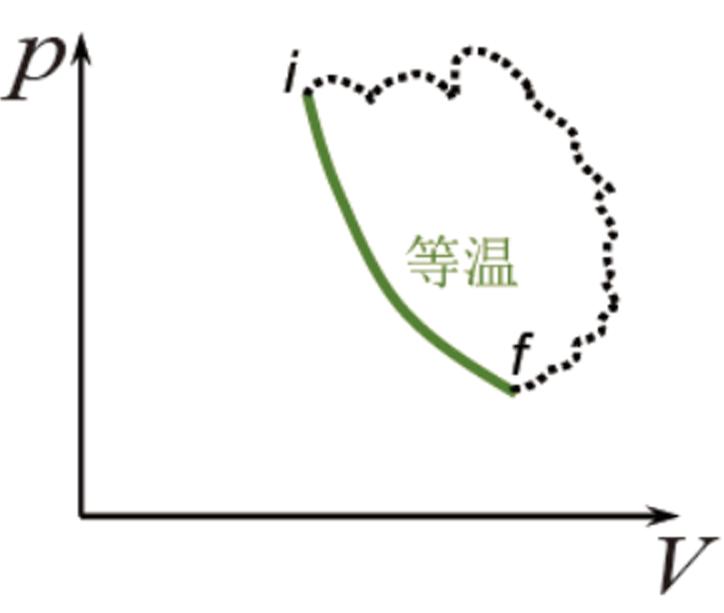
\includegraphics[width=0.4\textwidth]{free_expansion_entropy.png}
  \caption{自由膨胀过程熵变计算}
  \label{fig:free_expansion_entropy}
\end{figure}

\paragraph{气体混合过程的熵变}

设混合气体为理想气体，$c_j=\nu_j/\nu$ 是第 $j$ 种组分的摩尔百分比，温度为 $T$，体积为 $V$，压强为 $p=\sum_j p_j$，$p_j=c_j p$ 为第 $j$ 种组分的分压。

未混合时，各组分温度都是 $T$，压强都是 $p$，各自占有体积 $V_j=c_j V$。

\textit{计算途径 (1)：等温膨胀过程。}每个组分从 $V_j=c_j V$ 膨胀到 $V$：
\[
\Delta S_j=c_j\nu R\ln\frac{V}{V_j},\qquad
\Delta S=\sum_j\Delta S_j=-\nu R\sum_j c_j\ln\frac{V_j}{V}
\]
\[
\boxed{\Delta S=-\nu R\sum_j c_j\ln c_j>0}
\]

\textit{计算途径 (2)：等温变压过程。}每个组分从压力 $p$ 变化到 $p_j=c_j p$：
\[
\Delta S_j=-c_j\nu R\ln\frac{p_j}{p},\qquad
\Delta S=\sum_j\Delta S_j=-\nu R\sum_j c_j\ln\frac{p_j}{p}
\]
\[
\boxed{\Delta S=-\nu R\sum_j c_j\ln c_j>0}
\]

% ============================================================
\subsection{熵增加原理}
% ============================================================

\subsubsection{一般推导}

考虑孤立系统绝热过程的熵变。初态 $i$ 到末态 $f$ 有各种路径，设 $p$-$V$ 图上 $L$ 是讨论的过程（可逆或不可逆），选另一连接 $i$ 和 $f$ 的可逆路径 $L_0$，则 $(L+\text{逆}L_0)$ 构成一个循环。

由克劳修斯不等式：
\[
\oint\frac{\mathrm{d}Q}{T}=\int_L\frac{\mathrm{d}Q}{T}+\int_{-L_0}\frac{\mathrm{d}Q}{T}\le 0
\quad\Longrightarrow\quad
\int_L\frac{\mathrm{d}Q}{T}\le\int_{L_0}\frac{\mathrm{d}Q}{T}
\]

$i$ 到 $f$ 的过程中熵变为：
\[
\Delta S_L=\int_{L_0}\frac{\mathrm{d}Q}{T}\ge\int_L\frac{\mathrm{d}Q}{T}
\]

对绝热过程 $L$ 则有 $\Delta S_{ad}\ge\displaystyle\int_L\frac{\mathrm{d}Q}{T}=0$，即
\[
\boxed{\Delta S_{ad}\ge 0}
\]

% [插图：熵增加原理推导示意图]
\begin{figure}[htbp]
  \centering
  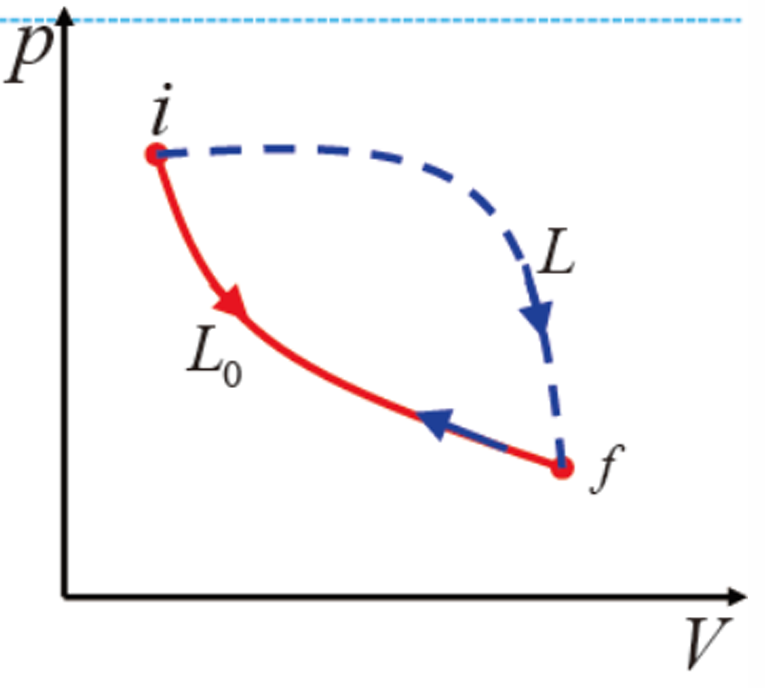
\includegraphics[width=0.4\textwidth]{entropy_increase.png}
  \caption{熵增加原理推导}
  \label{fig:entropy_increase}
\end{figure}

\subsubsection{熵增加原理的表述}

\textbf{热力学系统从一个平衡态经绝热过程到达另一个平衡态，它的熵永不减少。若过程可逆，则其熵不变；若过程不可逆，则其熵增加。}

\[
\boxed{\Delta S\ge 0}
\]

\paragraph{判断绝热过程是否可逆}
实际计算熵变：
\begin{itemize}[leftmargin=2em]
  \item 若 $\Delta S>0$ 则该绝热过程不可逆；
  \item 若 $\Delta S=0$ 则该绝热过程可逆。
\end{itemize}

\paragraph{克劳修斯不等式的另一种表述}
\[
\boxed{T\,\mathrm{d}S\ge \mathrm{d}Q}\quad(\text{可逆取等号})
\]

代入热力学第一定律，则有：
\[
T\,\mathrm{d}S\ge \mathrm{d}U-\mathrm{d}W=\mathrm{d}U+p\,\mathrm{d}V
\]

\subsubsection{讨论}

\begin{itemize}[leftmargin=2em]
  \item \textbf{熵增加原理}；
  \item 孤立系统绝热过程进行方向的判据（时间箭头）：$\Delta S\ge 0$；
  \item 孤立系统热平衡的判据：熵取得极大值，即 $\mathrm{d}S=0$；
  \item 严格地，在内能和体积不变的条件下，对于一切可能的变动来说，平衡态的熵最大，此时 $\mathrm{d}S=0$。
\end{itemize}

% ============================================================
\subsection{熵及热力学第二定律的统计意义}
% ============================================================

\subsubsection{玻尔兹曼熵}

\paragraph{定义}
\[
\boxed{S_B=k_B\ln\Omega}
\]
其中 $k_B$ 为玻尔兹曼常数，$\Omega$ 为系统的微观态数目。

\paragraph{分析}
热物理量可分为强度量和广延量两类，但 $\Omega$ 不能归入上述两类。然而：
\[
\ln\Omega_{A+B}=\ln(\Omega_A\cdot\Omega_B)=\ln\Omega_A+\ln\Omega_B
\]
即 $\ln\Omega$ 是\textbf{广延量}，且与 $\Omega$ 有相同的单调性质。所以可用上定义描述热力学系统的微观态及其性质。这样定义的 $S$ 即称为微观熵，或玻尔兹曼熵，记为 $S_B$。

\paragraph{宏观熵与微观熵的关系}
\[
\boxed{\Delta S_C=\Delta S_B}
\]

\subsubsection{熵的统计意义}

$\Omega$ 是系统的微观状态数，是系统内部无序程度的度量。所以，\textbf{熵是系统宏观状态对应的微观状态的多少（即无序程度）的度量}。

\begin{itemize}[leftmargin=2em]
  \item \textbf{熵高}意味着对应的微观状态数目多，即混乱、分散、无序程度高。根据\textbf{微观状态等几率基本假设}，微观状态数最多的宏观状态出现的概率最大；
  \item \textbf{熵低}意味着对应的微观状态数目少，即整齐、集中、无序程度低。根据微观状态等几率基本假设，微观状态数较少的宏观状态出现的概率较小；
  \item \textbf{熵增加}是系统从有序到无序的过程；其伴随的能量传递过程对应为有用（有序）能量减少，无用（无序）能量增多。
\end{itemize}

如：自由膨胀；扩散；固液、固气、液气相变；向米里掺沙子；功转变为热……

\subsubsection{热力学第二定律的统计意义}

对于孤立系统：
\[
S=k_B\ln\Omega,\qquad \Delta S=k_B\ln\frac{\Omega_f}{\Omega_i}
\]

由 $\mathrm{d}S\ge 0$，得 $\dfrac{\Omega_f}{\Omega_i}\ge 1$，孤立系统中自发的过程（不可逆），总有
\[
\boxed{\Omega_f\ge\Omega_i}
\]

\textbf{热力学第二定律的统计意义}：

\textbf{孤立系统的自发过程（不可逆过程）总是从有序向无序的过渡，即由出现概率小的宏观状态向出现概率大的宏观状态过渡。}


% ============================================================
\subsection{热力学系统态函数及其关系}
% ============================================================

\subsubsection{热力学势函数}

\paragraph{定义}
\begin{align*}
U&=U(T,V) &\text{（内能）}\\
H&=H(T,p)=U+pV &\text{（焓）}\\
S&=S(T,V) &\text{（熵）}\\
F&=U-TS &\text{（亥姆霍兹自由能）}\\
G&=H-TS &\text{（吉布斯自由焓）}
\end{align*}

\subsubsection{热力学基本方程（微分关系）}

将热力学第二定律 $\mathrm{d}S\ge\dfrac{\mathrm{d}Q}{T}$ 与热力学第一定律 $\mathrm{d}U=\mathrm{d}Q+\mathrm{d}W$ 联立：

\begin{center}
\begin{tabular}{c|c|c}
\hline
 & 可逆过程 & 不可逆过程 \\
\hline
$\mathrm{d}U$ & $T\,\mathrm{d}S-p\,\mathrm{d}V$ & $<T\,\mathrm{d}S-p\,\mathrm{d}V$ \\
$\mathrm{d}H$ & $T\,\mathrm{d}S+V\,\mathrm{d}p$ & $<T\,\mathrm{d}S+V\,\mathrm{d}p$ \\
$\mathrm{d}F$ & $-S\,\mathrm{d}T-p\,\mathrm{d}V$ & $<-S\,\mathrm{d}T-p\,\mathrm{d}V$ \\
$\mathrm{d}G$ & $-S\,\mathrm{d}T+V\,\mathrm{d}p$ & $<-S\,\mathrm{d}T+V\,\mathrm{d}p$ \\
\hline
\end{tabular}
\end{center}

\subsection{四个基本微分方程与八个一阶偏导数}

对于封闭系统（只考虑体积功），四个热力学势的全微分方程为：
\begin{align}
  \mathrm{d}U &= T\,\mathrm{d}S - p\,\mathrm{d}V \tag{1}\\[2pt]
  \mathrm{d}H &= T\,\mathrm{d}S + V\,\mathrm{d}p \tag{2}\\[2pt]
  \mathrm{d}F &= -S\,\mathrm{d}T - p\,\mathrm{d}V \tag{3}\\[2pt]
  \mathrm{d}G &= -S\,\mathrm{d}T + V\,\mathrm{d}p \tag{4}
\end{align}

由全微分表达式直接读出各热力学势对其自然变量的一阶偏导数（共八个）：

\begin{center}
\begin{tabular}{c|c|c}
\hline
热力学势 & 对第一自然变量的偏导 & 对第二自然变量的偏导 \\
\hline
$U(S,V)$ & $\displaystyle\left(\frac{\partial U}{\partial S}\right)_V=T$ & $\displaystyle\left(\frac{\partial U}{\partial V}\right)_S=-p$ \\[8pt]
$H(S,p)$ & $\displaystyle\left(\frac{\partial H}{\partial S}\right)_p=T$ & $\displaystyle\left(\frac{\partial H}{\partial p}\right)_S=V$ \\[8pt]
$F(T,V)$ & $\displaystyle\left(\frac{\partial F}{\partial T}\right)_V=-S$ & $\displaystyle\left(\frac{\partial F}{\partial V}\right)_T=-p$ \\[8pt]
$G(T,p)$ & $\displaystyle\left(\frac{\partial G}{\partial T}\right)_p=-S$ & $\displaystyle\left(\frac{\partial G}{\partial p}\right)_T=V$ \\
\hline
\end{tabular}
\end{center}

\subsection{熵关于温度的偏导数与热容}

利用链式法则与上述一阶偏导数，可得定容/定压热容与熵对温度偏导数的关系：
\[
C_V=\left(\frac{\partial U}{\partial T}\right)_V
=\left(\frac{\partial U}{\partial S}\right)_V\left(\frac{\partial S}{\partial T}\right)_V
=T\left(\frac{\partial S}{\partial T}\right)_V
\quad\Longrightarrow\quad
\boxed{\left(\frac{\partial S}{\partial T}\right)_V=\frac{C_V}{T}}
\]

\[
C_p=\left(\frac{\partial H}{\partial T}\right)_p
=\left(\frac{\partial H}{\partial S}\right)_p\left(\frac{\partial S}{\partial T}\right)_p
=T\left(\frac{\partial S}{\partial T}\right)_p
\quad\Longrightarrow\quad
\boxed{\left(\frac{\partial S}{\partial T}\right)_p=\frac{C_p}{T}}
\]

\subsection{麦克斯韦关系（Maxwell Relations）}

由解析函数（态函数）的混合偏导数与求导顺序无关，将四个基本微分方程分别应用于
$\displaystyle\frac{\partial^2 U}{\partial V\partial S}=\frac{\partial^2 U}{\partial S\partial V}$ 等，可得：

\begin{enumerate}[leftmargin=2em]
  \item \textbf{由 $\mathrm{d}U=T\,\mathrm{d}S-p\,\mathrm{d}V$}\\
  视 $U=U(S,V)$，则
  \[
  \boxed{\left(\frac{\partial T}{\partial V}\right)_S=-\left(\frac{\partial p}{\partial S}\right)_V}
  \]

  \item \textbf{由 $\mathrm{d}H=T\,\mathrm{d}S+V\,\mathrm{d}p$}\\
  视 $H=H(S,p)$，则
  \[
  \boxed{\left(\frac{\partial T}{\partial p}\right)_S=\left(\frac{\partial V}{\partial S}\right)_p}
  \]

  \item \textbf{由 $\mathrm{d}F=-S\,\mathrm{d}T-p\,\mathrm{d}V$}\\
  视 $F=F(T,V)$，则
  \[
  \boxed{\left(\frac{\partial S}{\partial V}\right)_T=\left(\frac{\partial p}{\partial T}\right)_V}
  \]

  \item \textbf{由 $\mathrm{d}G=-S\,\mathrm{d}T+V\,\mathrm{d}p$}\\
  视 $G=G(T,p)$，则
  \[
  \boxed{\left(\frac{\partial S}{\partial p}\right)_T=-\left(\frac{\partial V}{\partial T}\right)_p}
  \]
\end{enumerate}

\subsection{内能公式与焓公式}

\paragraph{内能公式}
以 $T,V$ 为独立变量，将熵的全微分
\[
\mathrm{d}S=\left(\frac{\partial S}{\partial T}\right)_V\mathrm{d}T
+\left(\frac{\partial S}{\partial V}\right)_T\mathrm{d}V
=\frac{C_V}{T}\,\mathrm{d}T+\left(\frac{\partial p}{\partial T}\right)_V\mathrm{d}V
\]
代入 $T\,\mathrm{d}S=\mathrm{d}U+p\,\mathrm{d}V$ 并比较 $\mathrm{d}V$ 的系数，得
\[
\boxed{\left(\frac{\partial U}{\partial V}\right)_T
=T\left(\frac{\partial p}{\partial T}\right)_V-p}
\]
此即\textbf{内能公式}。对理想气体 $p=\dfrac{\nu RT}{V}$，有 $\left(\dfrac{\partial p}{\partial T}\right)_V=\dfrac{\nu R}{V}$，代入得 $\left(\dfrac{\partial U}{\partial V}\right)_T=0$。

\paragraph{焓公式}
以 $T,p$ 为独立变量，将熵的全微分
\[
\mathrm{d}S=\left(\frac{\partial S}{\partial T}\right)_p\mathrm{d}T
+\left(\frac{\partial S}{\partial p}\right)_T\mathrm{d}p
=\frac{C_p}{T}\,\mathrm{d}T-\left(\frac{\partial V}{\partial T}\right)_p\mathrm{d}p
\]
代入 $T\,\mathrm{d}S=\mathrm{d}H-V\,\mathrm{d}p$ 并比较 $\mathrm{d}p$ 的系数，得
\[
\boxed{\left(\frac{\partial H}{\partial p}\right)_T
=-T\left(\frac{\partial V}{\partial T}\right)_p+V}
\]
此即\textbf{焓公式}。对理想气体 $V=\dfrac{\nu RT}{p}$，有 $\left(\dfrac{\partial V}{\partial T}\right)_p=\dfrac{\nu R}{p}$，代入得 $\left(\dfrac{\partial H}{\partial p}\right)_T=0$。

\subsection{化学势与开放系统}

对于封闭系统（$N=\text{const}$），$\mathrm{d}G=-S\,\mathrm{d}T+V\,\mathrm{d}p$。

对于开放系统，$G$ 是广延量，依赖于 $N$。对开放系统有
\[
\boxed{\mathrm{d}G=-S\,\mathrm{d}T+V\,\mathrm{d}p+\mu\,\mathrm{d}N}
\]
其中化学势定义为
\[
\boxed{\mu=\left(\frac{\partial G}{\partial N}\right)_{T,p}}
\]

推广到多组分系统，开放系统的四个热力学基本方程为：
\begin{align*}
  \mathrm{d}U &= T\,\mathrm{d}S-p\,\mathrm{d}V+\sum_i\mu_i\,\mathrm{d}N_i,\\
  \mathrm{d}H &= T\,\mathrm{d}S+V\,\mathrm{d}p+\sum_i\mu_i\,\mathrm{d}N_i,\\
  \mathrm{d}F &= -S\,\mathrm{d}T-p\,\mathrm{d}V+\sum_i\mu_i\,\mathrm{d}N_i,\\
  \mathrm{d}G &= -S\,\mathrm{d}T+V\,\mathrm{d}p+\sum_i\mu_i\,\mathrm{d}N_i.
\end{align*}

\subsection{相平衡条件}

在等温、等压条件下的平衡条件为 $\mathrm{d}G=0$。

对于两相系统（1, 2），有
\[
(\mathrm{d}G)_{T,p}=\mu_1\,\mathrm{d}N_1+\mu_2\,\mathrm{d}N_2=0
\]
相变中保持质量守恒：$N=N_1+N_2$，故 $\mathrm{d}N_1+\mathrm{d}N_2=0$。代入得
\[
\mu_1\,\mathrm{d}N_1=-\mu_2\,\mathrm{d}N_2=\mu_2\,\mathrm{d}N_1
\]
因此
\[
\boxed{\mu_1=\mu_2}
\]
\textbf{结论}：在相平衡中，各相物质的化学势相等。

\subsection{热力学第三定律}

\paragraph{能斯特定理}
系统的熵在等温过程中的改变随绝对温度趋于零：
\[
\boxed{\lim_{T\to 0}(\Delta S)_T=0}
\]

\paragraph{普朗克绝对熵}
任何纯物质在绝对零度时的熵值为零：
\[
\boxed{\lim_{T\to 0}S(T)=0}
\]

\paragraph{绝对零度不可达到}
由于制冷系数 $\varepsilon=\dfrac{T_2}{T_1-T_2}$，当 $T_2\to 0$ 时 $\varepsilon\to 0$。因此，
\textbf{不可能通过有限过程把一个物体的温度冷却到绝对零度}。这是热力学第三定律的另一个表述形式。


% ============================================================
\section{第六章补充：液体的表面性质与毛细现象}
% ============================================================

\subsection{表面张力系数与表面功}

对于由外力作用使液体表面积扩大的过程，外力作功为
\[
\mathrm{d}W=f\,\mathrm{d}x=\alpha\cdot 2l\,\mathrm{d}x=\alpha\,\mathrm{d}A_s
\]
其中 $\mathrm{d}A_s=2l\,\mathrm{d}x$ 为液面增加的表面积（注意薄膜有两个表面）。

表面张力系数定义为
\[
\boxed{\alpha=\frac{\mathrm{d}W}{\mathrm{d}A_s}}
\]
即\textbf{液面改变单位面积外界所作的功}（等温、等体条件下）。

\subsection{表面内能与表面内能密度}

对于表面系统，$F_s=F_s(A_s,T)=\alpha A_s$。由 $\mathrm{d}F_s=\alpha\,\mathrm{d}A_s-S\,\mathrm{d}T$ 及全微分表达式比较可得表面熵：
\[
S=-\left(\frac{\partial\alpha}{\partial T}\right)_{A_s}A_s
\]

表面内能 $U_s=F_s+TS$，故
\[
\boxed{U_s=\alpha A_s-TA_s\left(\frac{\partial\alpha}{\partial T}\right)_{A_s}}
\]
表面内能密度为
\[
\boxed{u_s=\alpha-T\left(\frac{\partial\alpha}{\partial T}\right)_{A_s}}
\]

\subsection{弯曲液面内外压强差（拉普拉斯公式）}

任意弯曲液面内外的压强差都可以表示为：
\[
\boxed{\Delta p=p_i-p_o=\alpha\left(\frac{1}{R_1}+\frac{1}{R_2}\right)}
\]
此即\textbf{拉普拉斯公式}（Laplace Formula）。

其中 $R_1,R_2$ 为过弯曲液面上一点的一对相互垂直\textbf{正截口}的曲率半径。
\textbf{曲率中心在液体内} $R>0$，\textbf{液体外} $R<0$。
正截口定义为：包含曲面法线的平面与曲面的交线。

\paragraph{简单讨论}
\begin{itemize}[leftmargin=2em]
  \item \textbf{球形液面}：$R_1=R_2=R$，则
  \[
  p_i-p_o=\frac{2\alpha}{R}
  \]
  \item \textbf{柱形液面}：$R_1=R,\ R_2=\infty$，则
  \[
  p_i-p_o=\frac{\alpha}{R}
  \]
\end{itemize}

液面形状由其内部、外部及表面三部分的平衡所决定：
\begin{itemize}[leftmargin=2em]
  \item 液面凸（曲率中心在液体内部）：$p_{\text{气}}<p_{\text{液}}$
  \item 液面凹（曲率中心在液体外部）：$p_{\text{气}}>p_{\text{液}}$
\end{itemize}

% [插图：球形液面与柱形液面压强差示意图]
\begin{figure}[htbp]
  \centering
  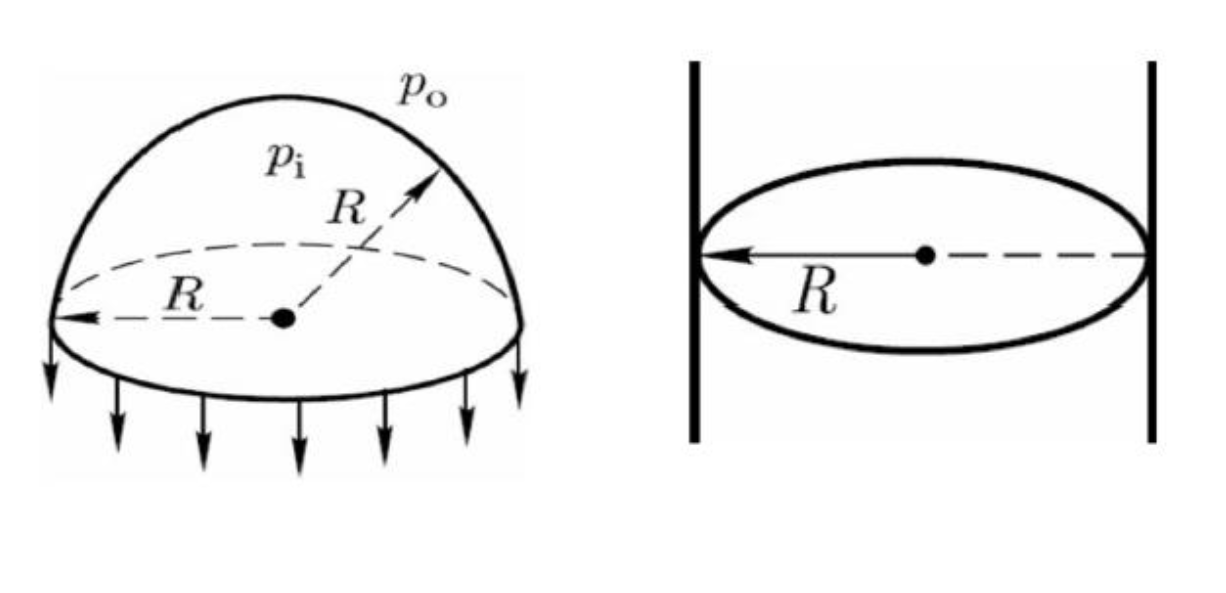
\includegraphics[width=0.4\textwidth]{laplace_discussion.png}
  \caption{球形液面与柱形液面压强差示意图}
  \label{fig:laplace_supplement}
\end{figure}

\subsection{毛细现象与液面高度}

\textbf{毛细现象}：将毛细管插入液体中，管内液面上升或下降的现象。

\textbf{物理根源}：液体的\textbf{内聚力}与\textbf{附着力}的竞争引起，由弯曲液面内外的压强差决定。

\begin{itemize}[leftmargin=2em]
  \item 附着力大于内聚力：液体\textbf{润湿}固体，液面上\textbf{凹}；液面``外''压强大于液面``内''压强，毛细管内液面\textbf{上升}。
  \item 内聚力大于附着力：液体\textbf{不润湿}固体，液面上\textbf{凸}；液面``内''压强大于液面``外''压强，毛细管内液面\textbf{下降}。
\end{itemize}

% [插图：毛细现象示意图，水在毛细管中上升、汞下降]
\begin{figure}[htbp]
  \centering
  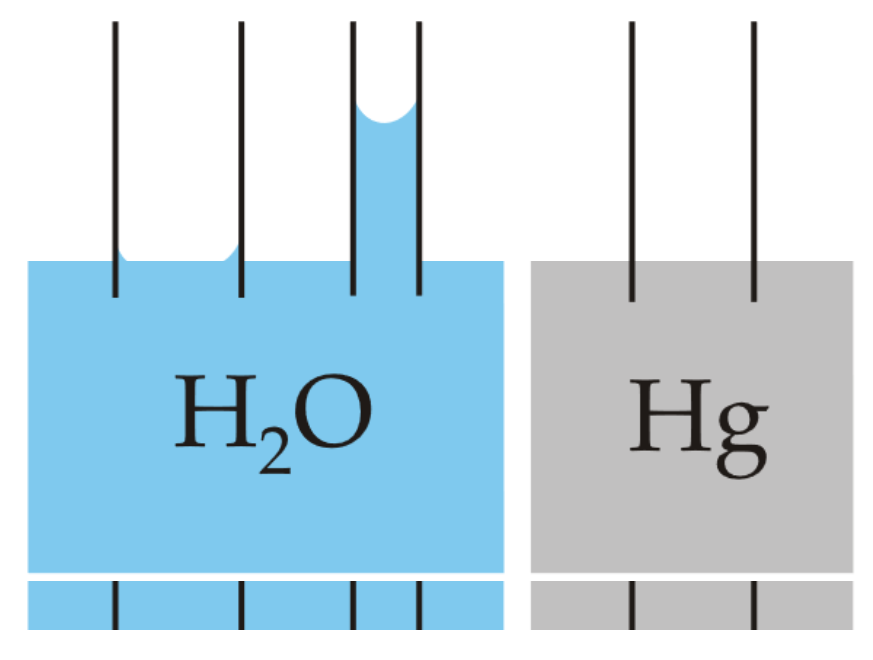
\includegraphics[width=0.4\textwidth]{capillary_tube.png}
  \caption{竖直毛细管中的润湿（水）与不润湿（汞）}
  \label{fig:capillary_supplement}
\end{figure}

\paragraph{液面高度公式}
柱形毛细管中，设管半径为 $r$，接触角为 $\theta$，则液面上升（或下降）高度为
\[
\boxed{h=\frac{2\alpha}{\rho gR}=\frac{2\alpha\cos\theta}{\rho gr}}
\]
其中 $R=r/\cos\theta$ 为液面曲率半径。

\begin{itemize}[leftmargin=2em]
  \item $0\le\theta<\pi/2\ \Rightarrow\ h>0$，内部液面上升；
  \item $\pi/2<\theta\le\pi\ \Rightarrow\ h<0$，内部液面下降。
\end{itemize}


% ============================================================
\section{第七章补充：相平衡与相图}
% ============================================================

\subsection{相平衡及相图}

\paragraph{相平衡}
相平衡是一个\textbf{动态平衡}。

\paragraph{相图}
把一物质系统的相、相变及相平衡以其状态参量为变量所作的图示，称为\textbf{相图}（phase diagram）。

典型单元系 $p$-$T$ 相图包含以下要素：
\begin{itemize}[leftmargin=2em]
  \item \textbf{汽化曲线}（$I$）：液气两相平衡共存曲线；
  \item \textbf{熔解曲线}（$II$）：固液两相平衡共存曲线；
  \item \textbf{升华曲线}（$III$）：固气两相平衡共存曲线；
  \item \textbf{三相点}（$\Theta$）：三条曲线交点，三相共存；
  \item \textbf{临界点}（$K$）：汽化曲线终点，对应临界温度 $T_c$。
\end{itemize}

% [插图：典型单元系相图 p-T 图]
\begin{figure}[htbp]
  \centering
  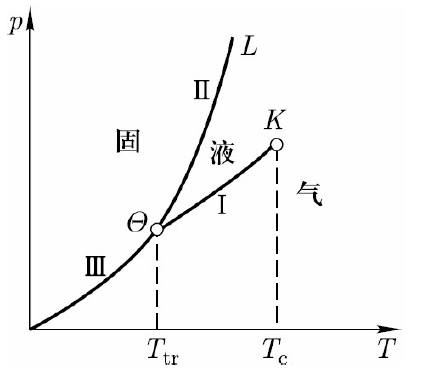
\includegraphics[width=0.5\textwidth]{phase_diagram.png}
  \caption{典型单元系相图（$p$-$T$ 图）}
  \label{fig:phase_diagram_supplement}
\end{figure}

\paragraph{临界温度}
在温度低于临界温度 $T_c$ 的情况下，系统可以发生有液气共存状态的一级相变（有摩尔体积突变）；而在 $T_c$ 之上，系统不再有液气共存的状态，即不再能发生一级相变。

\subsection{克拉珀龙方程}

对 $\alpha$ 相和 $\beta$ 相的两相系统，相平衡时 $\mu_\alpha(T,p)=\mu_\beta(T,p)$。当外界条件发生微小变化时，为保持平衡有 $\mathrm{d}\mu_\alpha=\mathrm{d}\mu_\beta$，即
\[
-S_{\alpha,m}\,\mathrm{d}T+V_{\alpha,m}\,\mathrm{d}p
=-S_{\beta,m}\,\mathrm{d}T+V_{\beta,m}\,\mathrm{d}p
\]

整理得相平衡曲线的斜率：
\[
\frac{\mathrm{d}p}{\mathrm{d}T}
=\frac{S_{\beta,m}-S_{\alpha,m}}{V_{\beta,m}-V_{\alpha,m}}
\]

在一级相变中，定义\textbf{摩尔相变潜热}：
\[
\boxed{\Lambda_m=T(S_{\beta,m}-S_{\alpha,m})}
\]

代入即得\textbf{克拉珀龙方程}（或克拉珀龙--克劳修斯方程）：
\[
\boxed{\frac{\mathrm{d}p}{\mathrm{d}T}
=\frac{\Lambda_m}{T(V_{\beta,m}-V_{\alpha,m})}}
\]

\paragraph{常见物质相变的相平衡曲线特征}
\begin{itemize}[leftmargin=2em]
  \item \textbf{汽化、升华过程}：$V_{\beta,m}>V_{\alpha,m}$，$\Lambda_m>0$，故 $\dfrac{\mathrm{d}p}{\mathrm{d}T}>0$。压强升高，沸点升高。
  \item \textbf{熔解过程（正常物质）}：$V_{\beta,m}>V_{\alpha,m}$，$\dfrac{\mathrm{d}p}{\mathrm{d}T}>0$。压强升高，熔点升高。
  \item \textbf{熔解过程（反常物质，如水）}：$V_{\beta,m}<V_{\alpha,m}$（冰熔解时体积减小），$\dfrac{\mathrm{d}p}{\mathrm{d}T}<0$。压强升高，熔点降低。
\end{itemize}

% [插图：常见物质相变的相平衡曲线示意图]
\begin{figure}[htbp]
  \centering
  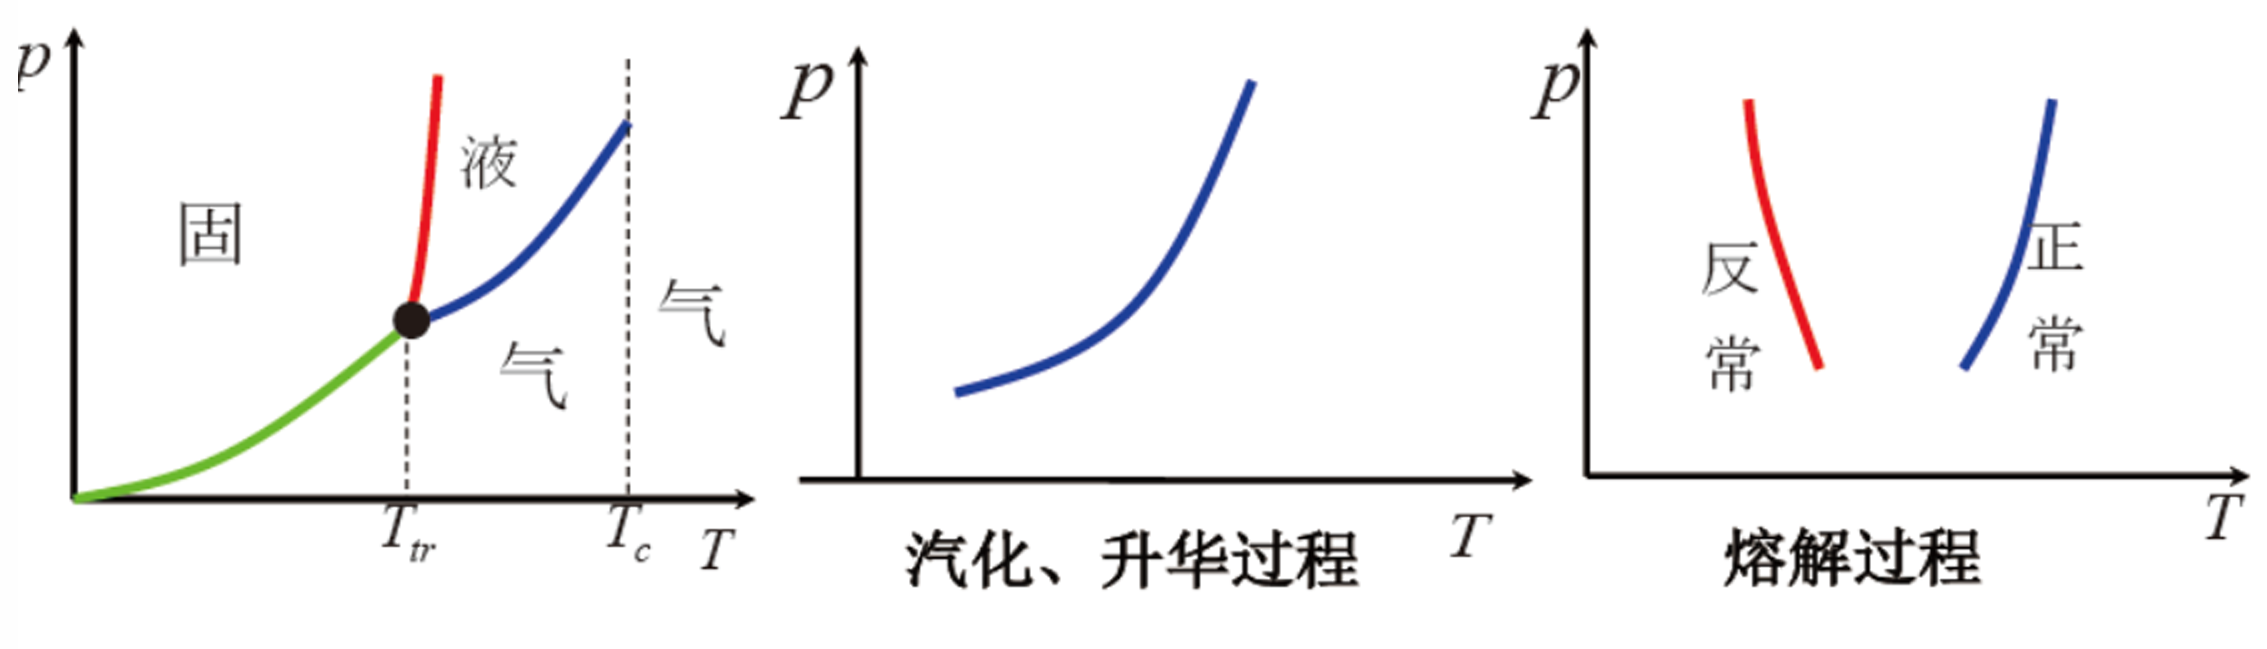
\includegraphics[width=0.8\textwidth]{clapeyron_curves.png}
  \caption{常见物质相变的相平衡曲线}
  \label{fig:clapeyron_curves_supplement}
\end{figure}


\end{document}